%%% Preamble %%%
\documentclass[a4paper,12pt]{report}
\usepackage{alltt}
\usepackage{amsfonts}
\usepackage{amsthm}
\usepackage{color}
\usepackage{epigraph}
\usepackage{float}
\usepackage{graphicx}
\usepackage{latexsym}						% Include extra symbols like \Box and \sqsubset
\usepackage{listings}
\usepackage{makeidx} \makeindex
\usepackage{setspace}
\usepackage{subfigure}
\usepackage{times}
\usepackage[notlof,nottoc]{tocbibind}	% Include the bibliography in the table of contents
\usepackage{url}
\usepackage{vmargin}

% Set the paper size and margins
\setpapersize{A4}
\setmargnohfrb{2cm}{2cm}{2cm}{2cm}

% Set the table of contents depth
\setcounter{tocdepth}{2}

% Change the line spacing
\doublespacing

% Prevent footnotes being split across multiple pages.
\interfootnotelinepenalty=10000

% Define new math operators
\newcommand{\argmax}{\mathop{\rm argmax}}
\newcommand{\argmin}{\mathop{\rm argmin}}
\newcommand{\diag}{\mathop{\rm diag}}

% Define the definition environment
\newtheorem{definition}{Definition}

% Define the thesis environment
\newtheorem*{thesis}{Thesis}

% Macros
\def\dx{\Delta x}
\def\dy{\Delta y}
\def\dz{\Delta z}
\def\dt{\Delta t}

\def\pd#1#2{\frac{\partial #1}{\partial #2}}						% partial derivative
\def\pdd#1#2{\frac{\partial^2 #1}{\partial #2^2}}				% partial second derivative
\def\pdk#1#2#3{\frac{\partial^#3 #1}{\partial #2^#3}}		% partial k'th derivative

\def\pdnf#1#2{\partial #1/\partial #2}									% partial derivative (no frac)
\def\pddnf#1#2{\partial^2 #1/\partial #2^2}							% partial second derivative (no frac)
\def\pdknf#1#2#3{\partial^#3 #1/\partial #2^#3}					% partial k'th derivative (no frac)

% Define a shorter way to add index entries
\newcommand{\stuidx}[2][\DefaultOpt]{\def\DefaultOpt{#2} \index{#1} \emph{#2}}

% Define a shorter way to include graphics.
\newcommand{\stufig}[4]
{
	\begin{figure}
	\begin{center}
		\includegraphics[#1]{#2}
		\caption{#3}
		\label{#4}
	\end{center}
	\end{figure}
}

\newcommand{\stufigex}[5]
{
	\begin{figure}[#5]
	\begin{center}
		\includegraphics[#1]{#2}
		\caption{#3}
		\label{#4}
	\end{center}
	\end{figure}
}

\newcommand{\stufignc}[2]					% images without captions
{
	\begin{figure}[H]
	\begin{center}
		\includegraphics[#1]{#2}
	\end{center}
	\label{fig:#2}
	\end{figure}
}

\begin{document}

% Setup before using the listings package
\renewcommand{\lstlistingname}{\textbf{Listing}}
\renewcommand{\thelstlisting}{\textbf{\arabic{lstlisting}}}

\definecolor{darkgreen}{rgb}{0, 0.6, 0}

\lstdefinelanguage{Pseudocode}{
morekeywords={break,continue,each,else,for,function,if,not,ref,return,then,var,while},
sensitive=true,
morecomment=[l]{//},
morecomment=[s]{/*}{*/}
}

\lstdefinestyle{Default}{
abovecaptionskip=0.5cm,
basicstyle=\scriptsize\ttfamily,
belowcaptionskip=0.5cm,
belowskip=0.5cm,
commentstyle=\color{darkgreen},
language=Pseudocode,
numbers=left,
numbersep=5pt,
numberstyle=\tiny,
mathescape=true,
showstringspaces=false,
stepnumber=1,
tabsize=4
}

\floatstyle{ruled}
\newfloat{stulisting}{thp}{lop}[chapter]
\floatname{stulisting}{Listing}

% Define extra colours
\definecolor{gold}{rgb}{0.75, 0.75, 0}
\definecolor{cyan}{rgb}{0, 0.75, 0.75}
\definecolor{purple}{rgb}{0.75, 0, 0.75}

%%% Top Matter %%%
\begin{titlepage}

\begin{center}

\vspace*{7.5cm}

\normalsize DPhil Thesis\\
\LARGE \textsc{Segmentation of Abdominal Organs and\\Growth Modelling of Tumours in\\Renal Cancer Patients}\\

\vspace{2mm}

\stufignc{width=3cm}{oxfclogos.jpg}

\vspace{-5mm}

\large Stuart M. Golodetz\\
\small stuart.golodetz@comlab.ox.ac.uk\\

\vspace{2mm}

\small Oxford University Computing Laboratory

\end{center}

\end{titlepage}

%%% Main Document %%%
\tableofcontents
\listoffigures
\listof{stulisting}{List of Code Listings}

% Get rid of the unnecessary space before chapter titles
\dropchapter{-2cm}

% Add page numbers
\pagestyle{plain}

% Stop the page numbers overlapping the text at the bottom of the page
\addtolength{\footskip}{7mm}

\begin{abstract}

This thesis focuses on how to allow a computer to identify features (such as major organs) in abdominal computerised tomography (CT) scans in an automatic way, whilst still facilitating user interaction with the results. Identifying such features is important if they are to be visualized in 3D for the purposes of diagnosis or surgical planning, or if their volumes are to be calculated when assessing a patient's response to therapy, but manual identification is time-consuming and error-prone. Some degree of computerised automation is therefore highly desirable, and indeed a small number of existing approaches have even attempted to fully automate the simultaneous identification of multiple abdominal organs. However, no existing method is capable of achieving results that are completely accurate in all cases, and due to the difficulties even of specifying when a result is correct, the development of such a method seems unlikely in the near future. It is thus important that medics retain the ability to correct the results when automated methods fail.

My research proposes a way of facilitating both automatic feature identification and intuitive editing of the results by representing CT images as a hierarchy of partitions, or \emph{image partition forest} (IPF). This data structure has appeared extensively in existing literature, but its potential uses for editing have hitherto received little attention. This thesis shows how it can be used for this purpose, by presenting a systematic set of algorithms that allow the user to modify the IPF, and select and identify features therein, via an intuitive graphical user interface. It further shows how such an IPF can be initially constructed from a set of CT images using morphological techniques, before presenting a series of novel methods for automatic feature identification in both 2D axial CT slices and 3D CT volumes.

%All of the techniques described have been implemented in one of two systems developed to illustrate their effectiveness. The trial system, \emph{centipede}, works on 2D slices, whilst the final system, \emph{millipede}, works on both 2D slices and 3D volumes. Validation tools were implemented in \emph{millipede} to allow the feature identification methods to be evaluated against `gold standard' manual results produced in collaboration with a radiologist, and the results are presented herein.

\end{abstract}


\part{Background}

%\chapter{Introduction}
\label{chap:introduction}

%The intertwined fields of segmentation and feature identification pose fundamental challenges in a variety of different domains. One such domain is that of image processing, in which the segmentation problem is first and foremost the task of partitioning an image into regions that correspond to `salient' features therein, although the term is also commonly used to refer to the related task of determining the boundary, or contour, around a feature of interest. The goal of feature identification, by contrast, is to assign semantic meaning to some or all of these regions.

In the most general sense, the problem of segmentation is the challenge of how to partition an object into pieces in such a way as to ensure that those pieces have some meaning in a given domain. The related (and to some extent overlapping) problem of feature identification is how to then ascribe meaning to some or all of those pieces. Whilst a huge variety of techniques have been developed for these problems, there are many domains in which it is difficult to specify, at least in a sufficiently precise manner, what constitutes a meaningful piece and what does not. For that reason both problems remain major research challenges.

Nevertheless, an ability to solve these problems, even in an imperfect way, is often a crucial precursor to applying other algorithms in various domains, making them worthy targets for research efforts. For example, in the medical imaging domain, it is helpful to be able to translate a volume of data produced by a scanner into a 3D mesh, allowing doctors to visualize the state of a patient's organs in a more direct manner. Whilst there are existing algorithms to convert \emph{labelled} volume data to a 3D mesh (e.g.~\cite{wu03}), these rely on a priori knowledge of the location of the organs. That is, they rely on the organs having being labelled in the volume in advance. Producing such a labelling is a segmentation and feature identification problem.

This thesis dissertation is about tackling the segmentation and feature identification problems for a particular type of medical image, namely computerised tomography (CT) scans of a patient's abdomen. The first practical CT scanner was originally developed in 1971 by Sir Godfrey Hounsfield, working at the EMI Central Research Laboratories in Hayes, UK. CT scanners work using X-rays (see Figure~\ref{fig:introduction-ctscanning}) and produce images whose pixels are scalar values on a scale of radiodensity known (after Sir Godfrey) as the Hounsfield scale. They are used extensively in modern medical practice, both for diagnosing illness and for evaluating a patient's response to therapy.

My underlying interest is in renal (kidney) cancers, in the diagnosis of which CT scanners are generally used to produce images of the abdomen (see Figure~\ref{fig:introduction-kidneyslocation}). Whilst less prevalent than some other types of cancer -- notably breast, lung, colorectal and prostate -- renal cancers nevertheless kill thousands of people a year in the UK.\footnote{According to Cancer Research UK \cite{cruk-kidneycancermortality}, 3752 people died from a kidney cancer in the UK in 2007, the most recent year for which published statistics are currently available.} An ability to visualize the state of a renal cancer patient's abdominal organs in 3D can provide doctors with an extra tool when making important decisions about how best to treat the patient. In a similar vein, being able to calculate the volume of a renal tumour can help doctors track changes over time that may be relevant when evaluating a patient's response to therapy. For these, and other, applications, finding a way to segment and identify features in abdominal CT scans is a key prerequisite.

%---
\section{The Niche}

TODO: Identify niche

\iffalse

\begin{itemize}

\item Attempts have been made to solve segmentation and feature identification in abdominal CT scans before, e.g.~...
\item But the limitations of these various methods are ...?
\item In other imaging subfields (including some of medical imaging) partition trees have been applied to good effect to represent images -- including some trees based on watershed (but not waterfall)
\item In some cases, attempts have been made to allow selection of regions in such a tree via cuts, etc.
\item What has not been done before is to build an explicit partition hierarchy using both the watershed and waterfall transforms and to use it (in combination with novel algorithms) to facilitate editing of segmentation results by the user
\item Furthermore, no-one has tried multi-layer region growing techniques for feature identification before (for that matter, I'm not sure they've tried multi-layer feature identification techniques period)
\item These, then, provide my `niche' (occupying it)
\item It is an interesting approach to try because it in principle combines the automation of morphological techniques with the previously untapped editing potential of partition hierarchies
\item Over the course of this dissertation, I will argue that it is also a useful approach, based on my results
\item Specifically, I aim to defend the thesis statement that...

\end{itemize}

\fi

%---
\section{Dissertation Organisation}

The remainder of this dissertation is organised as follows.

\textbf{Chapter~\ref{chap:background}} surveys the fields of segmentation and feature identification, and discusses some of the varied uses of partition hierarchies throughout computer science, with the intention of both placing my own techniques in context and providing the foundations for later discussion.

\textbf{Chapter~\ref{chap:methodology}} describes my research methodology in more detail, focusing in particular on the question of the appropriateness of my goals and the methods I chose to achieve them.

\textbf{Chapter~\ref{chap:ipfs}} describes partition forests, the key data structure I used to represent segmented images, and introduces novel algorithms I have developed for editing them and selecting nodes in multiple layers within them.

\textbf{Chapter~\ref{chap:segmentation}} shows how partition forests can be constructed from images using existing segmentation approaches such as the watershed and waterfall transforms. It looks at three different ways in which the waterfall transform can be implemented: an algorithm due to Marcotegui and Beucher \cite{marcotegui05}, a new tree-based algorithm due to my colleague Chris Nicholls \cite{nicholls09}, and my own novel tree-based approach, presented here for the first time, that handles minimal plateaux in a robust manner.

\textbf{Chapter~\ref{chap:featureid}} shows how feature identification algorithms, including a novel multi-layer region growing method, can be applied to the partition forest in order to automatically segment certain abdominal features. It also illustrates how the results of the segmentation and feature identification processes can be useful in solving real-world problems such as visualizing abdominal organs in three dimensions and calculating organ volumes.

\textbf{Chapter~\ref{chap:assessment}} assesses and validates the contributions made elsewhere in the dissertation (see below) and summarises my case supporting the thesis statement.

\textbf{Chapter~\ref{chap:conclusions}} discusses potential avenues for further work, and concludes the dissertation.

\textbf{Appendix~\ref{chap:datastructures}} provides information on basic structures such as disjoint set forests and minimum spanning trees.

\subsection{Contributions}

The original contributions made by this dissertation are:
%
\begin{enumerate}

\item Editing and selection algorithms for partition forests in Chapter~\ref{chap:ipfs}.
\item A simple edge-preserving image filter (known as a spatially-variant Gaussian filter), in \S\ref{subsec:segmentation-watershed-ct}.
\item A new algorithm for the waterfall transform in \S\ref{sec:segmentation-waterfall}.
%\item The adaptation of the watershed and waterfall algorithms to construct the partition forest in \S\ref{sec:segmentation-ipfconstruction}.
\item A new feature identification algorithm based on multi-layer region growing in the partition forest in Chapter~\ref{chap:featureid}.

\end{enumerate}
%
As noted above, these will be assessed in Chapter~\ref{chap:assessment}.
%\chapter{Literature Review}
\label{chap:background}

%---
\section{Chapter Overview}

In Chapter~\ref{chap:introduction}, the segmentation and feature identification problems were introduced, and my thesis was formally stated. This chapter surveys some of the wide variety of segmentation and feature identification techniques currently in use in the field of medical imaging, with the intention of providing the background necessary to place the specific techniques I used for my own work in context. It also surveys some of the uses of partition hierarchies (trees and forests) throughout computer science as a whole. This background lays the foundation for Chapter~\ref{chap:methodology}, in which the research approach I chose is discussed in the context of the overall goals of my doctoral work.

Whilst the segmentation and feature identification problems are theoretically distinct -- in that feature identification involves assigning semantic meaning to parts of an image where segmentation does not -- there is a great deal of overlap between them in practice. For example, the goal of some of the segmentation techniques we will see (e.g.~region growing) is to directly segment a particular feature of interest; in that sense, they are as much feature identification approaches as segmentation ones. For that reason, I have chosen to present the techniques used for both problems together, rather than separately.

The discussion of existing work on partition hierarchies foreshadows the formal definition of partition forests and the presentation of novel algorithms for working with them in Chapter~\ref{chap:ipfs}. Partition forests are a generalization of the partition trees that result from a certain type of bottom-up (merging-based) construction process, and the background on other areas where partition hierarchies are applied thus lays the groundwork for assessing the wider usefulness of my algorithms in Chapter~\ref{chap:assessment}.

%---
\section{Segmentation and Feature Identification}

\subsection{Overview}

The majority of the segmentation techniques in current use can be divided into eight classes: (1) thresholding techniques, which seek to segment an image based on dividing up the histogram of its grey values, (2) region growing techniques, which search for specific features by flooding outwards from one or more initial seed points in the image, (3) morphological techniques such as the watershed transform, which treats an image as a height map and divides it up into catchment basins that we try to ensure correspond to features of interest, (4) deformable models, which start with some arbitrary model of a desired feature and try to deform it to fit the image data, (5) learning techniques, which construct some variety of model based on a set of training images and use it to segment subsequent scans, (6) clustering techniques, which try and cluster objects (in this case image pixels) into groups whose members are mutually similar, but dissimilar to the members of other groups, (7) graph partitioning techniques such as the normalized cuts algorithm, and (8) hybrid techniques, which combine methods from the other classes to produce (what are hopefully good) results for specific applications. Each of these is discussed in more detail in one of the following subsections. The field as a whole is visually depicted in Figure~\ref{fig:background-segmentation-field}.

%---
\stufigex{height=16cm}{background/background-segmentation-field.png}{The field of image segmentation techniques}{fig:background-segmentation-field}{p}
%---

\subsection{Thresholding}

In principle, thresholding segmentation methods are quite simple. The idea is to divide the pixels of the image into classes through the use of one or more dividing lines on the image histogram. Dividing the image into two classes is known as \emph{binary thresholding}; where more classes are used, we refer to the process as \emph{multi-thresholding}. As an example, we could use binary thresholding to divide an 8-bit image (with grey levels ranging from $0 = \mbox{black}$ to $255 = \mbox{white}$) into two classes, one containing pixels greater than (say) $125$, and representing the foreground of the image, and the other containing all the remaining pixels and representing the background (see Figure~\ref{fig:background-segmentation-thresholding-binaryexample}).

%---
\begin{stusubfig}{p}
	\subfigure[The original image]
	{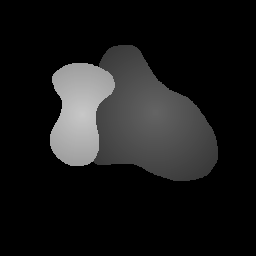
\includegraphics[height=.2\textheight]{background/background-segmentation-thresholding-binaryexample-a.png}}%
	%
	\hspace{4mm}%
	%
	\subfigure[The thresholded image]
	{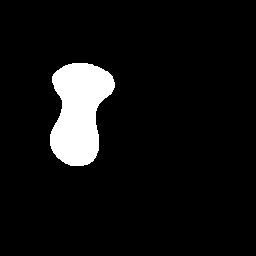
\includegraphics[height=.2\textheight]{background/background-segmentation-thresholding-binaryexample-b.png}}%
	%
	\hspace{4mm}%
	%
	\subfigure[The image histogram and threshold (at grey value $125$)]
	{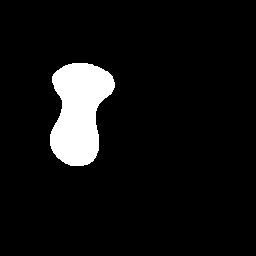
\includegraphics[height=.2\textheight]{background/background-segmentation-thresholding-binaryexample-c.png}}%
\caption{Segmenting the brighter of two adjacent objects in an 8-bit greyscale image using binary thresholding (the objects are easily separated in this case because the distribution of grey values in the image is bimodal)}
\label{fig:background-segmentation-thresholding-binaryexample}
\end{stusubfig}
%---

%---
\begin{stusubfig}{p}
	\subfigure[Segmenting Figure~\ref{fig:background-segmentation-thresholding-binaryexample}(a) with a threshold of $175$ leads to undersegmentation]
	{
\includegraphics[height=.2\textheight]{background/background-segmentation-thresholding-inaccurate-a.png}}%
	%
	\hspace{4mm}%
	%
	\subfigure[Conversely, segmenting it with a threshold of $75$ leads to oversegmentation]
	{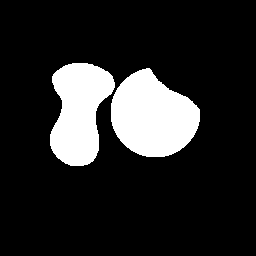
\includegraphics[height=.2\textheight]{background/background-segmentation-thresholding-inaccurate-b.png}}%
\caption{Misplaced thresholds lead to inaccurate segmentations}
\label{fig:background-segmentation-thresholding-inaccurate}
\end{stusubfig}
%---

\afterpage{\clearpage}

The difficulty encountered in practice is how to determine the optimum threshold location(s). A misplaced threshold will cause an inaccurate segmentation, so choosing the location appropriately is essential. In our example above, choosing a threshold that was too high would mean that the foreground of the image would be \emph{undersegmented} (i.e. pixels which should be classified as being part of the foreground are incorrectly classified as background) and the background would be \emph{oversegmented} (the converse) -- see Figure~\ref{fig:background-segmentation-thresholding-inaccurate}(a). Choosing too low a threshold would cause the opposite problem -- see Figure~\ref{fig:background-segmentation-thresholding-inaccurate}(b).

Owing to difficulties like this, applications are often designed so that thresholds can be chosen interactively by the user, but a great deal of work has also been done on automatically determining good threshold locations. As surveyed by Sezgin and Sankur in \cite{sezgin04}, there are six types of approach to the problem in current use:

\begin{enumerate}

\item \emph{Histogram shape-based methods.} These use shape properties of the histogram to find a good threshold. For instance, Rosenfeld's histogram concavity method, cited in \cite{lee.c92}, works by examining the difference between a histogram and its convex hull. A grey level at which the the height difference between the histogram and its convex hull is greatest (i.e. a point of deepest concavity) is picked as the threshold value.

\item \emph{Clustering-based methods.} These try and group the grey level data into a given number of clusters (two in the case of binary thresholding). One example is the method of Ridler and Calvard \cite{ridler78}. Their idea was to take a grey-level image and produce an initial binary classification which makes the assumption that the object of interest is somewhere in the middle of the image and the corners of the image contain only background. The means of the pixels currently classified as background and object are calculated and the average of the two means is taken. The new value is then used to threshold the image and produce a new binary classification into background and object classes: it is assumed that this will be more accurate than the initial guess. Finally, the process is iterated until there is little or no change in the binary classification, and the last threshold in the iteration is chosen for use.

\item \emph{Entropy-based methods.} These are based on information theory and pick thresholds by (for example) trying to maximise the information content in the thresholded image. As described by Wong and Sahoo in \cite{wong89}, the simplest possible such method looks at two probabilities, $F(T)$ and $F^*(T) = 1 - F(T)$, each parameterised in terms of a threshold, $T$. The first, $F(T)$, gives us the probability of a given pixel having a grey value less than or equal to the threshold, and the second, $F^*(T)$, gives us the probability of the value being greater than it. The information content in the thresholded image is given by
%
\[
H(T) = -F(T) \log_2 F(T) - F^*(T) \log_2 F^*(T)
\]
%
and attains a maximum when $F(T) = 0.5$. This is equivalent to saying that in the absence of any other knowledge, the maximum entropy principle tells us that the information contained in the thresholded image is maximised by picking a threshold which classifies half the pixels as background and half as foreground. This makes intuitive sense, but is too simplistic an approach for the majority of applications. Better alternatives have been developed (see \cite{sezgin04}), but are beyond the scope of this dissertation.

\item \emph{Object attribute-based methods.} These pick thresholds based on a comparison between the original grey-level image and the binarized (i.e.~segmented into two classes) version of it. For example, the method of Hertz and Schafer \cite{hertz88} picks the threshold that yields a binarized image whose edge field maximally corresponds to that of the original image. The edge fields in this case are obtained via the well-known Sobel operator \cite{gonzalez02}.

\item \emph{Spatial methods.} An example of a spatial thresholding method is Wu et al.'s approach in \cite{wu82}. This first constructs a quadtree from the image by splitting image regions until they have a low standard deviation (where they define `low' in terms of the standard deviation of the image as a whole). This divides the image into square blocks of various different sizes. The observation is that the smaller blocks tend to be near the boundaries between foreground and background in the image -- the quadtree can thus be used as a way of estimating where these boundaries are. Having classified the pixels in the image in this way, it is possible to construct a histogram of the grey values of non-boundary pixels in the image, which it is hoped will be more bimodal than the histogram of the grey values in the image as a whole. A threshold can then be placed at the deepest point in the value between the two modes. Alternatively, a histogram of the boundary pixels can be constructed, which it is hoped will be unimodal, and a threshold can be placed at the mean of this histogram instead.

\item \emph{Local / adaptive methods.} These vary the threshold for each pixel location in the image. Two examples of this are the methods of Bernsen \cite{bernsen86} and Niblack \cite{niblack86}. As described by Trier and Jain in \cite{trier95}, Bernsen's method takes the highest and lowest grey values, $g_{\mbox{max}}$ and $g_{\mbox{min}}$, in a suitably-sized window around each pixel, and uses them to calculate a contrast measure $C = g_{\mbox{max}} - g_{\mbox{min}}$. If $C$ is less than some user-specified value, the local neighbourhood around the pixel is taken to be uniform, and an appropriate choice is made about whether the pixel should be classified as background or foreground (in \cite{trier95}, pixels were always classified as background in this case). Otherwise, a threshold value $T = (g_{\mbox{max}} + g_{\mbox{min}}) / 2$ is calculated, and the pixel is classified as foreground if its value is greater than $T$, and background if not. Niblack's method, by contrast, bases its decision on the mean and standard deviation of the grey values in the local neighbourhood around a pixel. In particular, if $m$ is the local mean and $s$ the local standard deviation, Niblack's method calculates a local threshold $T = m + ks$, where $k$ is a (negative) user-specified parameter. Again, a pixel is classified as foreground iff its grey value is greater than $T$.

\end{enumerate}

\noindent In spite of the large amount of work done on thresholding, however, it has some significant downsides when used on its own to process medical images:

\begin{itemize}

\item It divides the image into two or more groups of pixels, based on their grey values, but there is no guarantee (or even an expectation) that any of these groups will be contiguous in the image. For instance, trying to segment a kidney from a CT scan by bounding it between two grey value thresholds might also result in inadvertently segmenting blood vessels across the image as well (their grey levels are quite similar to those of the kidneys). Not only are these blood vessels not part of the kidney, they are actually physically separated from it in the image! (It is also worth noting that trying to segment a kidney will generally result in segmenting both of them at once, since their grey level ranges are the same. This sort of problem can be overcome by specifying the side of the body in which we're interested.)

\item It is by no means the case that acceptable threshold locations always exist. If the grey value ranges of different objects of interest significantly overlap, it may be impossible to separate them using thresholding alone.

\end{itemize}

\noindent These limitations can in some cases be overcome by combining thresholding with other techniques. For instance, the results of thresholding often have gaps in them, which can sometimes be filled in by carefully applying various morphological operators (e.g. morphological opening and closing). Luc Soler's team \cite{soler01} made use of thresholding (as one technique among many) and achieved excellent automatic segmentation results for the liver. However, they did not use thresholding on its own. For instance, they segmented bones by thresholding for bright areas and then keeping only those which were near to the fat tissue (which had already been segmented). Simple thresholding alone would have been insufficient for the task, since structures such as the aorta also appeared bright on the contrast-enhanced images.

\subsection{Region Growing}

Region growing methods for segmentation essentially work as follows. First, an initial seed point is chosen for a feature of interest. Then, the region is `grown' by iteratively considering all points which are adjacent to the region and adding any which satisfy certain criteria (see Figure~\ref{fig:background-segmentation-regiongrowing-process}). For example, we could choose to add adjacent pixels whose grey value differs from that of their neighbour in the region by less than a certain amount. Alternatively, we could try and add adjacent pixels which preserve the homogeneity of the entire region (for some suitable definition of homogeneity) -- e.g.~Chen et al.\ \cite{chen09} define a criterion that leads an adjacent pixel to be added to the region provided that the absolute difference between its grey value and the mean grey value of the region is less than the standard deviation of the region's grey value distribution.

%---
\begin{stusubfig}{p}
	\subfigure[Initial state]
	{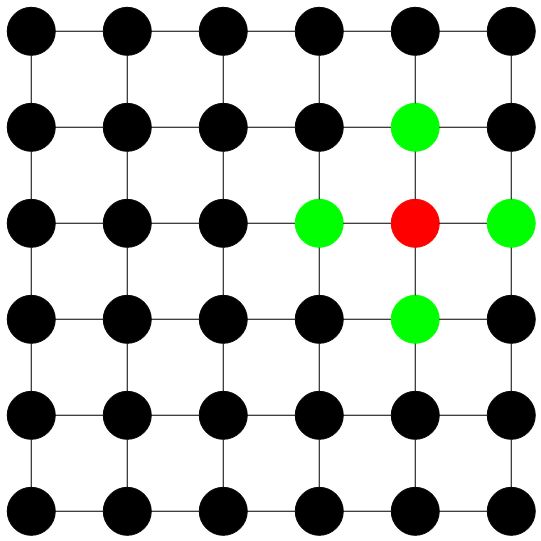
\includegraphics[height=5cm]{background/background-segmentation-regiongrowing-process-a.png}}%
	%
	\hspace{12mm}%
	%
	\subfigure[After one iteration]
	{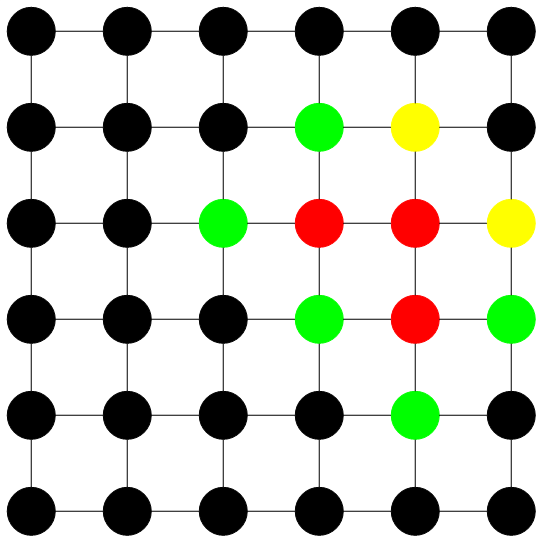
\includegraphics[height=5cm]{background/background-segmentation-regiongrowing-process-b.png}}%
	%
	\\ \vspace{12mm}
	%
	\subfigure[After two iterations]
	{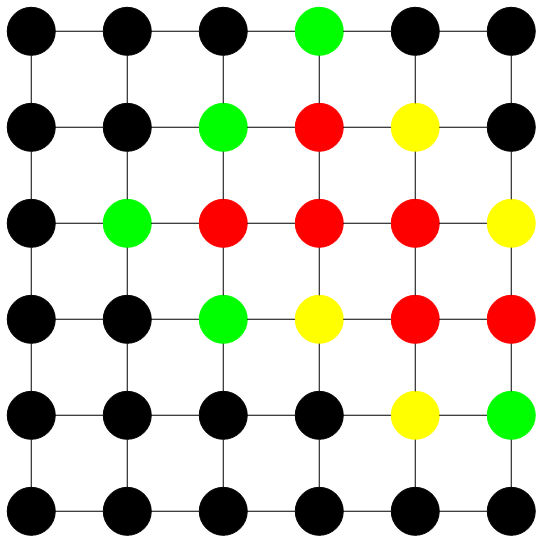
\includegraphics[height=5cm]{background/background-segmentation-regiongrowing-process-c.png}}%
	%
	\hspace{12mm}%
	%
	\subfigure[Final state]
	{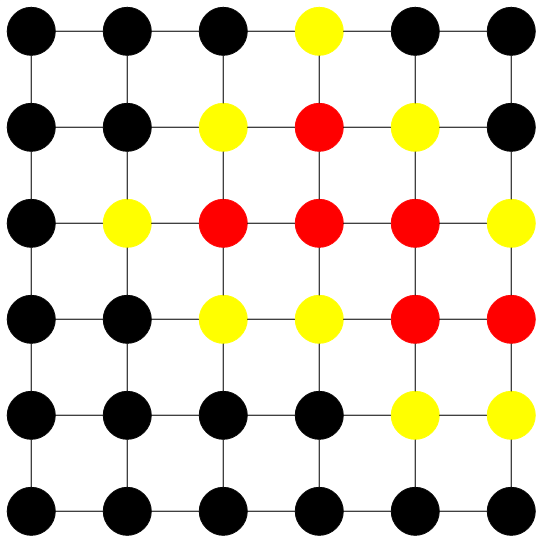
\includegraphics[height=5cm]{background/background-segmentation-regiongrowing-process-d.png}}%
\caption{An example region growing process -- black pixels are those not yet considered, red pixels are those currently in the region, green pixels are those under consideration, and yellow pixels are those that already failed the similarity criterion. The algorithm terminates when there are no further pixels to consider. The final segmented object is shown in red in (d).}
\label{fig:background-segmentation-regiongrowing-process}
\end{stusubfig}
%---

%---
\begin{stulisting}[p]
\caption{A Generic Region Growing Algorithm}
\label{code:background-segmentation-regiongrowing-generic}
\begin{lstlisting}[style=Default]
function grow_region
: (seed : PixelCoords; criterion : PixelCoords $\to$ bool) $\to$ Set<PixelCoords>

	var queue : Queue<PixelCoords>;
	var result, visited : Set<PixelCoords>;

	// Add the seed point to the queue and mark it as visited.
	queue.push(seed);
	visited.insert(seed);

	while not queue.empty()
		p := queue.pop();
		result.insert(p);

		// Add neighbours satisfying the similarity criterion to the queue.
		for each neighbour $\in$ neighbours(p)
			if not visited.contains(neighbour) then
				if criterion(neighbour) = true then queue.push(neighbour);
				visited.insert(neighbour);
			
	return result;
\end{lstlisting}
\end{stulisting}
%---

More involved criteria are also possible. One popular approach is that of \emph{adaptive} region growing (e.g.~see \cite{lin06,pohle01}), whereby the criterion varies to take account of the area around the pixel under consideration. In \cite{lin06}, for example, the approach taken is as follows. After locating an initial seed point $(s_x, s_y)$, a $7 \times 7$ mesh is placed over it and the maximum and minimum pixel intensities within the mesh, $M(s_x, s_y)$ and $m(s_x, s_y)$ are determined. From these, a contrast range $t_0 = M(s_x, s_y) - m(s_x, s_y)$ is calculated and recorded. Next, for each pixel $(x,y)$ under consideration for addition to the region, values $M(x,y)$ and $m(x,y)$ are similarly calculated, and a local value $\theta_{\rm local} = (M(x,y) + m(x,y)) / 2$ is determined. The region growing criterion is then formulated as $|f(x,y) - \theta_{\rm local}| \le t_0$, i.e. we add an adjacent pixel $(x,y)$ to the region if the absolute difference between its grey value $f(x,y)$ and the midpoint of the contrast range of the $7 \times 7$ mesh surrounding it is less than the contrast range of the $7 \times 7$ mesh centred on the initial seed point. The region growing is specified to stop when this absolute difference is greater than a certain threshold, implying that the area surrounding a given pixel is not homogeneous.

A generic region growing algorithm can be implemented straightforwardly using a queue (see Listing~\ref{code:background-segmentation-regiongrowing-generic}). Starting from a queue containing only the initial seed point, we repeatedly pop the pixel at the front of the queue, consider its non-region neighbours for addition to the region, and push any which satisfy the requisite criteria onto the end of the queue. The process terminates when the queue empties.

The key policy issues to consider when implementing region growing are how to choose the seed point, how to formulate the criteria specifying which points to add to the region, and how to decide when the process should terminate. For automated segmentation methods, how to choose the seed point is of fundamental importance; semi-automated algorithms can focus exclusively on the latter two problems, relying instead on the user to interactively specify an initial seed.

The advantages of region growing methods are that the resultant region is guaranteed to be connected in the image (unlike with thresholding) and that they are, on the whole, fairly easy to implement. However, from the point of view of automatic segmentation, they present difficulties, because choosing an initial seed point is in general a non-trivial problem. The usual approach taken for automatic seed point selection is to rely on statistical data about where the features of interest (e.g. organs) usually lie in the body. For instance, the approach in \cite{lin06} is to search for suitable seed points in two elliptical regions on each side of the body, one for each kidney. This worked quite well in context, but is not robust in the general case, relying strongly on the kidneys being in the expected places -- for example, it is unsuitable for MRI images, in which the patient's body may be oriented arbitrarily. It would also fail if used for images of auto-transplant patients.

Whilst region growing algorithms are guaranteed to produce a connected result, the region may still have holes in the middle of it. Whilst this may be desirable if we really are trying to segment a torus-shaped feature, on the whole it is necessary to post-process the region growing results to remove these holes, e.g.~using morphological closing techniques.

\subsection{Morphological Techniques}

Mathematical morphology is a large and rather general field based on lattice theory \cite{goutsias00}. It contains many useful image processing techniques, the majority of which are not relevant for the purposes of this survey, but in segmentation terms its key technique is the watershed transform, originally developed by Serge Beucher \cite{beucher90}.

The watershed, which will be described in substantially more detail in Chapter~\ref{chap:segmentation}, is essentially a technique for dividing landscapes into their catchment basins (where a catchment basin is an area of the landscape from which water would run down to a given local minimum) -- see Figure~\ref{fig:background-segmentation-watershed-concept}. In imaging terms, this can be utilised for segmentation purposes by treating an image as a discrete landscape and pre-processing it so as to try to establish a correspondence between catchment basins in the landscape and features of interest in the image. If such a correspondence can be successfully established, finding the catchment basins then equates to finding the desired image features.

%---
\stufigex{width=9cm, height=9cm}{segmentation/segmentation-watershed-concept.png}{The watershed transform constructs watersheds (the red partitions) that divide a landscape into its catchment basins}{fig:background-segmentation-watershed-concept}{p}
%---

Many image algorithms have been developed to actually perform the watershed transform; in general, these can be classified as either flooding algorithms (e.g.~\cite{bieniek00,rambabu07}) or rainfalling algorithms (e.g.~\cite{meijster98,osma-ruiz06,stoev00}). The former essentially flood out from the local minima in the landscape and (implicitly or otherwise) add watershed boundaries where the different catchment basins meet; the latter determine paths of steepest descent from points in the landscape and assign them to catchment basins based on the local minima to which their paths lead down.

In practice, however, it is rarely possible to establish a perfect correspondence between the catchment basins in the landscape and the desired features in the image, as to do so consistently would require prior knowledge of where the desired features actually are in the image, which would defeat the point of segmenting the image in the first place. One of the most common problems encountered with the watershed transform is that of oversegmentation: the landscape fed into the watershed has an excess number of catchment basins, most of which do not correspond to anything of interest in the actual image. This is particularly true of landscapes representing noisy images -- small changes in grey values can create shallow catchment basins, or dimples, in the landscape, greatly affecting the resulting segmentation.

There are two main approaches in the literature for dealing with this problem, namely marker imposition (leading to an approach known rather aptly as `watershed-from-markers') and hierarchical segmentation. Marker imposition essentially works by specifying markers on particular features of interest a priori, and flooding out only from those. This partitions an image into a number of regions equal to the number of specified markers and thereby solves the oversegmentation problem. Unfortunately, it can be extremely difficult to determine the required markers automatically -- rather than solving the underlying problem, we have merely changed it into one of marker determination. This may or may not prove problematic, depending on the data available and the specifics of the application. In some cases, it may be possible to use other data to determine marker placement automatically -- for example, Grau et al.\ \cite{grau04} successfully used a statistical atlas for this. In other cases, it may simply be acceptable to place the markers manually \cite{xue05}, or to initially place them manually and then propagate them from one image in a sequence to the next \cite{flores09}.

In situations where neither is the case, however, the alternative approach of hierarchical segmentation can be used. As one might expect, the general idea here is to take the oversegmented result of running the watershed transform on an image, and perform several iterations of region merging to produce a hierarchy of gradually coarser partitions of the original image. As will be illustrated in far more detail in Chapter~\ref{chap:segmentation}, this is exactly the sort of approach taken by the waterfall transform \cite{beucher90,marcotegui05}: what is unique about the waterfall, however, is that each of its iterations in which it merges regions together is itself a watershed transform.

As will be discussed in Chapter~\ref{chap:methodology}, the hierarchical approach to watershed segmentation is interesting for a couple of reasons: on the one hand, it produces, without requiring a great deal of manual fine-tuning, segmentations which, whilst not perfect, are often quite reasonable to a first approximation; on the other hand, the hierarchy of partitions of the image it produces can be turned into a tree structure (see \S\ref{sec:background-partitionhierarchies}) which is amenable to further editing, allowing any flaws in the initial segmentation to be corrected in an intuitive manner. These two qualities make this approach eminently suitable in situations where automated solutions are desirable but interactive control remains important.

\subsection{Deformable Models}

As their name suggests, deformable models methods work by taking an initial model of the features under consideration and deforming it to fit the actual data available. The initialisation of the model is generally based on \emph{a priori} anatomical knowledge. The model itself can be represented in a variety of ways, and these ways correspond to a number of different approaches to the problem. For example, the snakes method, which we will see shortly, represents the model as a parametrically-defined spline, and is hence referred to as an example of a parametric deformable model (it is sometimes also referred to as an explicit deformable model). In contrast, level sets represent the model \emph{implicitly} and are an example of implicit deformable models. Implicit deformable models were developed later than their parametric counterparts, but both types see a lot of use.

\subsubsection{Parametric Deformable Models}

\paragraph{Snakes}

As originally defined by Kass, Witkin and Terzopoulos in \cite{kass88}, `A snake is an energy-minimizing spline guided by external constraint forces and influenced by image forces that pull it toward features such as lines and edges.' Essentially, the idea works as follows. We represent the position of the snake, in terms of a spline parameter $s$, as $\mathbf{v}(s) = (x(s),y(s))$, and define an \emph{energy functional}, $E_{snake}^*$, as
%
\[
E_{snake}^* = \int_0^1 E_{int}(\mathbf{v}(s)) + E_{image}(\mathbf{v}(s)) + E_{con}(\mathbf{v}(s)) \; ds.
\]
%
The three terms in the summation are \emph{internal} energy, which tries to limit the curvature of the snake, \emph{image} energy, which tries to attract the snake towards features in the image such as lines and edges, and \emph{constraint} energy, which allows the user to apply constraints to influence the result of the segmentation. The snake algorithm as a whole attempts to find a spline minimising $E_{snake}^*$.

The original snakes paper describes a continuous model, but more recent research \cite{lobregt95,miller90b,miller90a} has seen the development of discrete models as well. The model described by Lobregt and Viergever in \cite{lobregt95}, called a \emph{discrete dynamic contour model}, is particularly interesting, and worth describing in more detail. Rather than relying on ideas of energy-minimization, Lobregt and Viergever model snakes using a force-based physical simulation. In their approach, a snake is a set of vertices connected by edges. At each time-step, various forces are applied to each vertex, which gradually \emph{deform} the snake towards the desired result. The results of this approach will depend to an extent on the lengths of the edges joining the vertices: if an edge is too long, important image features may pass through the gaps between vertices; if it is too short, the snake may become overly fixated on small details, not to mention the speed of the process being adversely affected. For this reason, after each deformation step, the snake is \emph{resampled} (by adding or removing vertices where necessary) to keep the edge lengths within certain limits.

The forces applied to each vertex closely mimic the energy terms in the original snakes paper. The force $\mathbf{f_i}$ applied to vertex $i$ is defined as the weighted sum
%
\[
\mathbf{f_i} = w_{ex}\mathbf{f_{ex,r_i}} + w_{in}\mathbf{f_{in,i}} + \underbrace{w_{damp}}_{< \; 0}\mathbf{v_i},
\]
%
where $\mathbf{f_{ex,r_i}}$ is an \emph{external} force term corresponding to the image and constraint terms from the original formulation, $\mathbf{f_{in,i}}$ is an \emph{internal} force term corresponding to the original internal term, and the remaining term is a new addition used to apply damping to try and bring the simulation to rest. (The real numbers $w_{ex}$, $w_{in}$ and $w_{damp}$ specify the weights to be given to each of these three factors. The paper tended to set all three of these to $0.5$: apparently this was derived empirically.)

It is important to mention that the method relies on quite a close initialisation (i.e.~image features have quite a short capture range). In \cite{ree05}, this problem is circumvented by peforming a watershed-from-markers segmentation and using the result of that to initialise the snake. Another alternative, referred to there, is to try and add additional external forces to solve the problem: in particular, some success has been had with \emph{balloon forces} \cite{cohen91} and \emph{gradient vector flow} (GVF) \cite{xu98}. For example, Figure~\ref{fig:background-segmentation-snakes-gvfexample} shows a GVF snake successfully segmenting the left ventricle of a human heart.

%---
\stufigex{height=9cm}{background/background-segmentation-snakes-gvfexample.png}{The basic snakes method suffers from a poor capture range, but techniques such as gradient vector flow \cite{xu98} can mitigate this -- the figure (reproduced from the paper in question) shows a GVF snake deforming from an initial, circular contour to segment the left ventricle of a human heart }{fig:background-segmentation-snakes-gvfexample}{p}
%---

Problems of this kind with snakes methods have led to a great deal of interest in level sets as an alternative, although snakes also remain popular as a well-established and far simpler alternative. They also have the advantage that they can represent open structures as well as closed ones.

\paragraph{NURBS-Based}

Another type of parametric deformable model, this time based on non-uniform rational B-splines (NURBS), is described by Tsagaan et al.\ \cite{tsagaan02}, in which they use a 3D NURBS-based model of a kidney and deform it by minimizing an energy function. Their results seem good in some cases, but differ markedly from the manually segmented results they show in others.

\subsubsection{Implicit Deformable Models}

\paragraph{Level Sets}

Curves and surfaces in general can be specified either explicitly (such that they can be calculated directly from the definition) or implicitly (the opposite). For instance, an explicit (parametric) representation of a circle in terms of its radius $r$ and an angle $\theta$ might be:
%
\begin{eqnarray*}
x & = & r \cos \theta \\
y & = & r \sin \theta
\end{eqnarray*}
%
The corresponding implicit representation would be:
%
\[
x^2 + y^2 = r^2
\]
%
As we have seen, parametric deformable model approaches like snakes represent their model using the former approach. Level set approaches, by contrast, use the latter. As an introduction to the ideas behind level sets, consider the function $\psi(x,y) = x^2 + y^2$, which defines a scalar field over $\mathbb{R}^2$. For any value $k > 0$, the equation $\psi(x,y) = k$ defines a circle in the x-y plane: we will refer to each of these circles as an \emph{isosurface} of $\psi$, because each of them is the surface (curve) of all the points at which $\psi$ takes a particular value.\footnote{\emph{Iso} means `equal' in Greek, so here we are talking about the surface containing all the points with the same $\psi$ value.} The key idea is that if we now change $\psi$, for instance by redefining it as $\psi(x,y) = x^3 + y^3$, the isosurfaces change, in this case from circles to hypercircles. Thus by changing the function $\psi$, we can move the isosurfaces of $\psi$ around without ever having to represent them explicitly. Level set approaches make use of this by representing the deformable model as an isosurface of some function $\psi$, and then modifying $\psi$ to deform the model towards the boundary of the desired image feature.

%---
\stufigex{height=6cm}{background/background-segmentation-levelsets-circleexample.png}{A simple circular contour which gradually expands over time}{fig:background-segmentation-levelsets-circleexample}{p}
%---

%---
\stufigex{height=6cm}{background/background-segmentation-levelsets-ellipseexample.png}{An example of a contour which changes its shape over time}{fig:background-segmentation-levelsets-ellipseexample}{p}
%---

%---
\stufigex{height=6cm}{background/background-segmentation-levelsets-uniformgrid.png}{Approximating a function $\psi(\mathbf{x},t)$ with a discrete, uniformly-spaced grid (note that the time superscripts on the grid values are not shown)}{fig:background-segmentation-levelsets-uniformgrid}{p}
%---

To represent contour changes over time, level set approaches make $\psi$ a function of time as well, and define it over some domain $U \subset \mathbb{R}^N$, giving us $\psi(\mathbf{x}, t) : U \times \mathbb{R}^+ \rightarrow \mathbb{R}$. They then set this equal to some constant (generally $0$) to actually specify one of the isosurfaces of $\psi$ as the contour being deformed. As a simple example of this, consider a circle, centred at the origin, which gradually expands outwards as the time increases (see Figure~\ref{fig:background-segmentation-levelsets-circleexample}). Supposing its radius to be $t$ at time $t$, we could represent this as:
%
\[
\psi((x,y),t) = x^2 + y^2 - t^2 = 0
\]
%
A more complicated example might involve gradually changing the circle into an ellipse over time (see Figure~\ref{fig:background-segmentation-levelsets-ellipseexample}). This could be achieved by writing:
%
\[
\psi((x,y),t) = x^2 + (yt)^2 - t^2 = 0
\]
%
Thus far, we have examined the basic ideas underpinning level sets, but not seen how they can be applied to the practical problem of segmentation. A common approach of real-world level set methods is to take as input not an explicit function of the kind we have just seen, but an initial contour on the image. This will then be deformed (using numerical methods) over time to try and fit it to an image feature of interest. There are thus six essential questions to consider:

\begin{enumerate}

\item How do we represent the function $\psi$?

\item Given an initial contour by the user, how do we use it to construct the initial function $\psi(\mathbf{x}, t = 0)$?

\item How do we define a numerical method to deform the initial function over time?

\item How do we know when the algorithm has terminated?

\item How do we extract the contour of interest over time?

\item How do we try and make the algorithm segment the desired image feature?

\end{enumerate}

\noindent To answer these questions, we consider the level set approach of Malladi et al., described in \cite{malladi95}. There, as tends to be the case for level set approaches in general, the function $\psi$ is represented by storing a discrete grid of approximate values over the domain $U$. The grid is uniformly-spaced, with squares of side $h$ (see Figure~\ref{fig:background-segmentation-levelsets-uniformgrid}). Each grid node has (for each integer value of $n \ge 0$) an associated value $\psi_{ij}^n$, which approximates the value $\psi((ih,jh),n\dt)$, where $\dt$ is the time step of the numerical method that will be used to deform the initial contour over time.

The initial goal is to construct, from a contour specified by the user, the grid of values $\psi_{ij}^0$ approximating the function $\psi(\mathbf{x},0)$. In \cite{malladi95}, this is done by setting $\psi_{ij}^0$ to be the signed distance of the grid node $ij$ from the initial contour (points outside the contour are assigned positive values and those inside are assigned negative ones) -- see Figure~\ref{fig:background-segmentation-levelsets-initialfunction}.

%---
\stufigex{height=7cm}{background/background-segmentation-levelsets-initialfunction.png}{Generating the initial function from the zero contour specified by the user (in red)}{fig:background-segmentation-levelsets-initialfunction}{p}
%---

Having constructed the grid for the initial function, the next step is then to define an appropriate numerical method to deform it over time. To do this, we first need a partial differential equation for $\psi$. The appropriate PDE, as derived in \cite{malladi95}, is:
%
\[
\pd{\psi}{t} + F|\nabla \psi| = 0
\]
%
Here, $F$ is called the \emph{speed function}, and will be used to control how $\psi$ evolves in a manner that will be discussed below. This can be approximated numerically as
%
\[
\frac{\psi_{ij}^{n+1} - \psi_{ij}^n}{\dt} + (F)(\nabla_{ij} \psi_{ij}^n) = 0,
\]
%
where (as noted, and described in more detail, in the paper), $\nabla_{ij} \psi_{ij}^n$ is `some appropriate finite difference operator for the spatial derivative'. This equation can be iteratively solved using standard numerical techniques (e.g.~see \cite{morton05}) and used to deform the model over time. The algorithm terminates when the contour of interest no longer changes between iterations.

To extract the contour of interest after each iteration, Malladi et al. construct a piecewise linear approximation to it, the gist of which involves finding the squares where some of the corner values are positive and some are negative, and constructing line segments therein. This bears not a little resemblance to the marching squares algorithm, the 2D analogue of marching cubes \cite{lorensen87}.

The remaining issue is how to use this algorithm to actually segment features in an image. For this, we make use of the speed function $F$, which controls how the contour deforms. Malladi et al.\ go into great detail about how $F$ should be defined, but essentially the idea is to define it so as to have (a) an advection component -- basically a term providing a constant speed inwards or outwards, (b) an image component -- a term which tries to make the contour move quickly when it is not near potential feature boundaries and slowly when it is close to them, and possibly (c) a geometry component -- a term which aims to control the local curvature of the contour. For the two-component version, with only an advection and an image component, this corresponds to an equation of the form
%
\[
\pd{\psi}{t} + (F_A + \hat{F}_I)|\nabla \psi| = 0,
\]
%
where $F_A$ is the advection component and $\hat{F}_I$ is the image component. For the version with a geometry component as well, the equation becomes
%
\[
\pd{\psi}{t} + \hat{k}_I(F_A + F_G)|\nabla \psi| = 0,
\]
%
where $F_G$ is the geometry component and $\hat{k}_I$ fulfils the role of the image component in the previous equation. The detailed definitions of the various components can be found in \cite{malladi95}. It is worth noting that this term-based approach bears a lot of similarity to that used for snakes, and in general the motivations for the various terms are more or less the same in each case.

Level sets have a number of advantages over snakes. One advantage is that they handle topological changes in an extremely simple fashion. For instance, consider Figure~\ref{fig:background-segmentation-levelsets-topologychanges}(a), in which the isosurface $\psi = 4$ is divided into two separate components. This is seamlessly represented by a level set approach, since it merely has to maintain a grid of numbers and not one or more explicit curves. Furthermore, the number of components can evolve over time without any special handling being required: in Figure~\ref{fig:background-segmentation-levelsets-topologychanges}(b), a change to the value of a single grid point can merge the two separate components into one, changing the topology at a stroke without any fuss. A corresponding implementation with snakes would involve far more work.

%---
\begin{stusubfig}{p}
	\subfigure[An isosurface divided into two separate components]
	{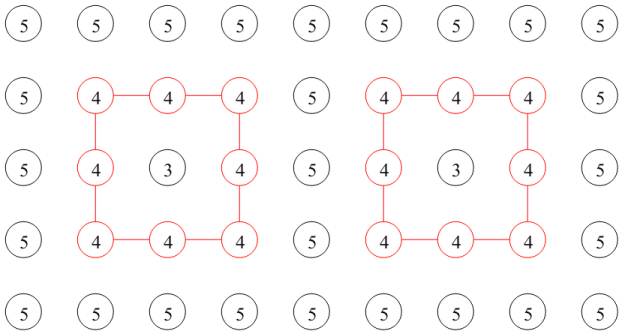
\includegraphics[height=6cm]{background/background-segmentation-levelsets-topologychanges-a.png}}%
	%
	\\ \vspace{4mm}%
	%
	\subfigure[Changing a single grid value merges the two components into one]
	{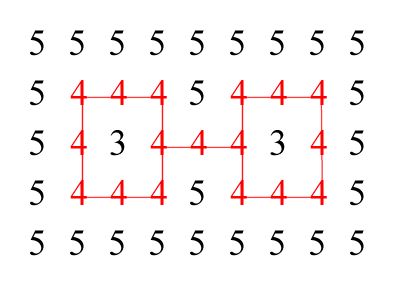
\includegraphics[height=6cm]{background/background-segmentation-levelsets-topologychanges-b.png}}%
\caption{Level set approaches seamlessly handle multiple boundaries and changes in topology}
\label{fig:background-segmentation-levelsets-topologychanges}
\end{stusubfig}
%---

Another advantage of level sets is that, unlike snakes, they translate straightforwardly into three dimensions -- all that is required is to replace a 2D grid with a 3D one. It is worth remarking, however, that the extra processing involved in the 3D case is substantial, making the basic scheme described above unsuitable if timely solutions are required. Special techniques have been developed to deal with this problem. One example is the narrow-band technique mentioned in \cite{malladi95}, which essentially restricts numerical calculations to a narrow regions around the isosurface in which we're particularly interested (i.e.~the one representing the deformable model). The insight is that solving the PDE over the whole domain is only necessary if we're interested in solving for the entire family of isosurfaces associated with $\psi$: often, we're only interested in a single isosurface, so the extra computations aren't necessary. More details of this sort of technique are available in \cite{malladi95} and \cite{itk}.

\subsubsection{Other Deformable Models}

Although parametric and implicit models are the most common types of deformable model in use, there are some techniques which do not fall into either category. Two techniques in particular are worth briefly mentioning. In \cite{jalba04}, Jalba et al.\ use a deformable model based on charged particles to achieve some interesting automatic segmentation results. There, the model is represented neither parametrically nor implicitly, but instead as a set of charged particles under the influence of an electrostatic field. Another interesting type of deformable model is the m-rep, described by Pizer et al.\ in \cite{pizer03}. This uses a medial representation of the model.

\subsection{Learning Techniques}

Learning segmentation techniques generally start with a training phase, in which a large number of scans are taken and used to construct some variety of model, which encodes information that can be used to segment subsequent scans. Two different types of learning technique will be discussed in the following subsections.

\subsubsection{Atlas-Based Techniques}

Atlas-based methods start by constructing an atlas, or reference segmentation, from a set of training data. For instance, in \cite{park03}, Park et al.\ constructed a probabilistic atlas by registering (aligning) the manually segmented volumes of 31 patients onto that of a carefully chosen reference patient (thus the data came from 32 patients in all). The atlas was represented as a 3D grid of vector values, where the components of each vector corresponded to the organs under consideration, and the values of the components indicated the fractional percentage of registered data sets in which the point was labelled as the given organ. As an example, if we were considering the liver and the two kidneys, the vector $(0.4, 0.6, 0)^T$ at a point could indicate that the point was inside the liver in 40\% of the data sets and inside the right kidney in 60\% of them.

After constructing such an atlas, new sets of data can be segmented by registering them onto it. In \cite{park03}, they use a \emph{maximum a posteriori} (MAP) approach after registration to find the segmentation result which best explains the observed data. The important point here is that the segmentation result is based on both the data for the individual patient and the information encoded in the atlas. The atlas provides the prior probabilities at each voxel, and these are refined in light of the actual patient data.

To use the notation in \cite{park03}, we denote the segmentation result field as $\mathbf{X}$, the field of observed data for the individual patient as $\mathbf{Y}$, and the probabilistic atlas as $\mathbf{A}$. Each of these represents a volume of $N$ voxels, indexed linearly (in some order) from $1$ to $N$. So for instance, a particular segmentation result could be given by $\mathbf{x} = (x_1, x_2, \ldots, x_N)$. Our aim is to find the best possible $\mathbf{x}$, defined as
%
\[
\mathbf{\hat{x}} = \argmax_{\mathbf{x}} \mathbf{P}(\mathbf{X} = \mathbf{x} | \mathbf{Y} = \mathbf{y}).
\]
%
In other words, we seek the segmentation result which best explains the observed patient data, $\mathbf{y}$. The probabilistic atlas is used in all of this as the prior for $\mathbf{X}$. Suppose there are $L$ different possible voxel labels, numbered from $1$ to $L$. Each voxel $a_i$ of the probabilistic atlas contains an $L$-vector, $(a_{i,1}, \ldots, a_{i,L})$, where $a_{i,\ell}$ gives the probability of a voxel's correct label being $\ell$. We use this to define the prior probabilities for $\mathbf{X}$, writing
%
\[
P(x_i = \ell) = a_{i,\ell}.
\]
%
In other words, the probability of the correct segmentation result for a given voxel being $\ell$ is given by the $\ell^{th}$ component of the probabilistic atlas at that location. With this link made, the result determined will depend on both the atlas and the observed data.

\subsubsection{Neural Network Techniques}

Neural networks (NNs) can be used to segment images in a number of ways. A simple NN technique can be found in \cite{tsai94}, where Tsai and Tanahashi use a feed-forward network to classify each pixel into one of three classes (liver, boundary or non-liver) according to the grey-level histogram of the 7x7 region centred on the pixel. (In practice, they use a histogram with 16 grey levels instead of 256, to avoid a proliferation of input nodes in the NN.) The schematic of how this works (borrowed from their paper) is shown in Figure~\ref{fig:background-segmentation-neuralnets-tsai}. The NN is initially trained by picking a suitable image from the middle of the volume and marking a significant number of training regions for each class. The well-known back-propagation algorithm for NNs \cite{aima} is used to update the weights on the network arcs accordingly.

%---
\stufigex{height=20cm}{background/background-segmentation-neuralnets-tsai.png}{Schematic diagram of the neural-network-based boundary detection method used in \cite{tsai94} (reproduced from the paper in question)}{fig:background-segmentation-neuralnets-tsai}{p}
%---

A more up-to-date (and more complicated) NN scheme can be found in \cite{lee03}. Here, Lee et al.\ use a multi-module, recurrent neural network to segment multiple abdominal organs (see Figure~\ref{fig:background-segmentation-neuralnets-lee}). There is a module associated with each label under consideration. Each node of a given module $k$ corresponds to a pixel in the image and encodes the probability that the pixel should be assigned label $k$. The weights of the network arcs are initially derived from (for example) a correlation matrix containing the likelihoods of various labels occurring next to each other. (For example, the liver might be quite likely to occur next to the right kidney, but definitely shouldn't occur next to the left kidney.) An iterative state evolution algorithm is used to determine the probabilities at each node in each of the modules of the NN. The initial probabilities are generated using something called the `Kohonen self-organizing algorithm' (see the paper for details) and the nodes are updated at each time step based on the current probability at a given node and the support it receives from its neighbours. (So, for instance, if a pixel was currently classified as part of the left kidney, but all its neighbours were liver, it would be very likely to change to liver over time.) The results of this method (after combining it with fuzzy spatial rules for organ identification) are quite good -- see Figure~\ref{fig:background-segmentation-neuralnets-leeresults}.

%---
\stufigex{height=8cm}{background/background-segmentation-neuralnets-lee.png}{The architecture of the contextual neural network used in \cite{lee03} (reproduced from the paper in question)}{fig:background-segmentation-neuralnets-lee}{p}
%---

%---
\stufigex{height=8cm}{background/background-segmentation-neuralnets-leeresults.png}{Results of the neural network method described in \cite{lee03} (reproduced from the paper in question), showing the identified spine, left kidney, spleen and liver}{fig:background-segmentation-neuralnets-leeresults}{p}
%---

%\subsubsection{Statistical Methods}

%TODO: \cite{touhami05}

\subsection{Clustering}

Clustering is the general problem of how to collect objects into groups in such a way that the members of each group are (with relation to application-specific criteria) similar to each other, but dissimilar to those in other groups. This can evidently be applied to image segmentation, with the goal of clustering the image into groups of similar pixels.

\subsubsection{K-Means}

A generalised description of the K-means approach to clustering is that it aims to divide a set of $n$ objects $\{o_1,\ldots,o_n\}$ into $k \le n$ groups $G = \{G_1,\ldots,G_k\}$ in such a way as to minimise the sum of squares of some measure of similarity $m$ between each object and the `mean' of the objects of its group. (At this stage of the description, what is meant by the mean in this instance is left deliberately under-specified.) More formally, if $\mu_j$ is the mean of the objects in group $G_j$, K-means aims to find a set of groups $G$ minimising:
%
\[
\sum_{j=1}^k \sum_{o \in G_j} m(o, \mu_j)^2
\]
%
The method generally used to try and find $G$ is an heuristic known as Lloyd's algorithm \cite{lloyd82} (which, it must be remarked, may be difficult to discern from the original paper). This works as follows:

\begin{enumerate}

\item An initial set of $k$ means are chosen, either manually, randomly or otherwise.

\item Each object (in the case of imaging, each pixel) is assigned to the group to whose mean it is closest, i.e.~object $o$ is placed in the group with index:
%
\[
\argmin_{i=1}^k m(o, \mu_i)
\]

\item The means for all groups that have changed since the last iteration are recalculated.

\item Steps 2 and 3 are repeated until no groups change between one iteration and the next.

\end{enumerate}

\noindent Lloyd's algorithm is not guaranteed to find the global optimum for $G$, but it has been shown by Arthur and Vassilvitskii \cite{arthur07} that a careful choice of the initial means can make the algorithm $O(\log k)$-competitive with the optimal clustering.

The key issues when using Lloyd's algorithm to segment images are how to define both the similarity measure and the mean of a set of objects. In some domains, the similarity measure can simply be defined as the distance between objects, and the mean as the average of the objects' positions, but for images this may not produce good results. Instead, similarity measures can be defined which are based not only on the positions of the pixels, but also on their values (for example, see \cite{?}). In such cases, the way in which the mean of a set of objects is defined will vary accordingly.

It should be noted that each cluster produced by this simple k-means approach is highly unlikely to be contiguous in the image (see Figure~\ref{fig:background-segmentation-kmeans-noncontiguity}). Some attempts have been made to address this in the literature (e.g.~see \cite{luo03,ilea06}).

\subsubsection{Fuzzy C-Means}

Fuzzy C-means is essentially a fuzzy relative of the K-means approach just described. It was originally presented by Dunn in 1974 \cite{dunn74}. The key idea is that instead of objects being divided crisply into groups (i.e.~each object belonging completely to exactly one group), objects have a degree of membership for each group. Using the same notation as before, and letting $u_{ij}$ be a real number between $0$ and $1$ indicating the degree to which object $o_i$ is a member of group $G_j$, and $1 \le p < \infty$ be a real parameter (e.g.~$p = 2$), we seek to find a set of groups $G$ minimising:
%
\[
\sum_{j=1}^k \sum_{o_i \in G_j} u_{ij}^p \cdot m(o,\mu_j)^2
\]
%
The standard algorithm for fuzzy C-means is once again an iterative, heuristic method:

\begin{enumerate}

\item Initialise the $u_{ij}$ values for the first iteration (written as ${}^{(0)}u_{ij}$). Any of the initialisation approaches which work for K-means will work equally well for this (i.e.~it suffices to pick an initial set of means and assign objects completely to their nearest groups by setting the $u_{ij}$ value to $1$ for their group and $0$ for all other groups).

\item At iteration $s$, calculate the updated means of the groups using the equation:
%
\[
\mu_j^{(s)} = \frac{\displaystyle \sum_{o_i \in G_j} {}^{(s-1)}u_{ij}^p \cdot o_i}{\displaystyle \sum_{o_i \in G_j} {}^{(s-1)}u_{ij}^p}
\]

\item Calculate the updated values ${}^{(s+1)}u_{ij}$ using the equation:
%
\[
{}^{(s+1)}u_{ij} = \frac{1}{\displaystyle \sum_{j=1}^k \left( \frac{m(o_i, \mu_j)}{m(o_i, \mu_k)} \right)^{\frac{2}{p-1}}}
\]

\item Iterate Steps 2 and 3 until
%
\[
\max_{ij} |{}^{(s+1)}u_{ij} - {}^{(s)}u_{ij}| < \epsilon,
\]
%
where $\epsilon$ is a real number between $0$ and $1$.

\end{enumerate}

\noindent Once again, as with Lloyd's algorithm for K-means, this is not guaranteed to produce the global optimum.

\subsection{Graph Partitioning}
\label{subsec:graphpartitioning}

Graph partitioning segmentation algorithms work by representing an object to be segmented as a weighted, undirected graph. In the case of images, the nodes of this graph would be the pixels of the image, and each of its edges would connect a pair of adjacent pixels and be weighted according to some measure of the dissimilarity between those pixels (one possible definition, based on both the pixel values and their spatial location in the image, appears in \cite{shi00}). The idea is then to find a good way to partition the nodes of the graph into pieces. For instance, if $G = (V,E,w)$ is a graph with vertex set $V$, edge set $E$ and weight function $w$, the \emph{minimum cut} approach seeks to partition $V$ into two disjoint sets $A$ and $B$ such as to minimise:
%
\[
\mbox{cut}(A,B) = \sum_{u \in A, v \in B} w(u,v)
\]
%
As mentioned by (among others) Shi and Malik in \cite{shi00}, however, the minimum cut approach tends to partition the graph so as to cut away small groups of poorly connected nodes, with undesirable results. Instead, they define, and then try to minimise, a measure of the lack of quality of a binary partition called the \emph{normalized cut}, namely
%
\[
\mbox{Ncut}(A,B) = \frac{\mbox{cut}(A,B)}{\mbox{assoc}(A,V)} + \frac{\mbox{cut}(A,B)}{\mbox{assoc}(B,V)},
\]
%
where they define $\mbox{assoc}(X,V) = \sum_{u \in X, t \in V} w(u,t)$ for both $X = A$ and $X = B$. This solves the aforementioned problem with the minimum cut approach, because if (for example) $A$ is a small group of poorly connected nodes, we would expect $\mbox{cut}(A,B)$ to be almost the same as $\mbox{assoc}(A,V)$, leading to a large value for $\mbox{Ncut}(A,B)$.

Finding a good partition given the definition of a normalized cut involves solving an eigenvalue problem, the details of which are described in \cite{shi00}. Having solved the eigensystem, we take the second smallest eigenvector (for reasons discussed in the paper) and use it to try and compute a good partition. The eigenvector will have one real-valued component for each pixel in the image -- the idea is to find a splitting point which minimises the value of the normalized cut. Assuming the values are relatively well separated into two distinct clusters, this can be done by checking the cut value for a number of evenly-spaced, real-valued potential cut points, and picking the one with the lowest value. Pixels with values above the cut then form one group, and those with values below the other. If the values are not well separated, however, the cut values may well be similar for several different cut points. For that reason, \cite{shi00} defines a stability criterion which essentially measures the reliability of the cut.

The binary partitioning process thus far described then becomes part of a recursive partitioning scheme. Starting with the whole image, as good a binary partition as possible of the current image region is computed, along with the stability of the cut. If the stability is too low, the image region is not partitioned. Otherwise, the value of the cut itself is considered. If it is too high (i.e.~greater than some user-specified threshold), the recursion terminates. Otherwise, the binary partitioning process is repeated on the two sub-regions just computed. Via this recursive process, the image as a whole is partitioned into a number of groups dependent on the maximum allowed cut value and the stability criterion.

\subsection{Hybrid Techniques}

It is sometimes possible to achieve better results by combining a number of different segmentation methods than it is by using a single method on its own. A striking example of how successful this sort of technique can be seen in the work of Luc Soler et al.\ \cite{soler01}, in which they describe an extensively hybrid technique for automatic segmentation of the liver from spiral CT scans. Their segmentation method first uses thresholding, morphological operators and distance maps to identify the skin, bones, lungs, kidneys and spleen. They next use a clever deformable model approach to embed a reference model of the liver into the image and automatically deform it to the liver contours. Later stages use Gaussian fitting on the image histogram to separate normal liver tissue from blood vessels and lesions (tumours), a result which is further refined by their own analytical methods. The final stage of their method makes use of higher-level medical knowledge to label the hepatic portal vein and segment the liver automatically according to an anatomically-based definition by Couinaud \cite{couinaud57}. The results of this technique are excellent -- see Figure~\ref{fig:background-segmentation-hybrid-soler}.

%---
\stufigex{height=8cm}{background/background-segmentation-hybrid-soler.png}{An automatic 3D reconstruction of patients from medical images, as performed by the IRCAD surgical planning tools developed using the work of Luc Soler et al.\ (the figure is reproduced from \cite{soler-imvie})}{fig:background-segmentation-hybrid-soler}{t}
%---

Other hybrid methods can be found in e.g.~\cite{ng06} and \cite{itk}. In \cite{ng06}, Ng et al.\ precede a watershed segmentation of MRI images of the head with a K-means clustering step -- this has the effect of hugely reducing the oversegmentation that the watershed would otherwise produce. It is a method that works particularly well for head segmentation, where the number of clusters is well-known a priori (in this case, the authors note that the types of tissue present tend to be `bone, soft tissue, fat and background'). There are several hybrid segmentation methods in \cite{itk}: in one, the authors combine fuzzy connectedness, Voronoi diagram classification and deformable models; in another, they combine Gibbs priors and deformable models. The details of these techniques are beyond the scope of this dissertation, but an implementation of the methods can be found in the freely-available \emph{Insight Toolkit}.

\clearpage

%---
\section{Partition Hierarchies}
\label{sec:background-partitionhierarchies}

%TODO: (i) Brief description of what a partition tree is; (ii) Explain, with suitable references, the various situations in which they are used; (iii) Narrow it down to images and survey the various techniques, noting the key differences between the representations (e.g.~whether or not adjacency information is maintained, etc.); (iv) Explain (at a high level) how partition forests fit into the picture

\subsection{Overview}

Partition hierarchies comprise two related data structures -- partition trees and partition forests. A \emph{partition tree} is a tree-based data structure containing nodes that represent portions of an entity, and satisfying the condition that the sub-entities represented by the children of any node in the tree partition the sub-entity represented by that node -- that is, the child sub-entities together form the parent sub-entity, and none of the child sub-entities mutually overlap. (I will henceforth, for reasons of brevity, refer to nodes partitioning each other, rather than referring to the sub-entities they represent.) An example of a partition tree can be seen in Figure~\ref{fig:background-partitionhierarchies-treeexample}. Partition forests will be discussed below (and in Chapter~\ref{chap:ipfs}).

%---
\stufigex{height=8cm}{todo.png}{TODO}{fig:background-partitionhierarchies-treeexample}{p}
%---

Partition trees can be either incomplete or complete. An incomplete partition tree is one with an incomplete lowest layer, and a complete one is the opposite. Complete partition trees have the property that the nodes in any given layer form a partition of the entity as a whole. For either type of tree, this is also true of the set of leaf nodes (those nodes without children). It should be noted that every incomplete partition tree has an equivalent complete partition tree. This can be constructed by adding a chain of nodes downwards from every leaf which is not in the lowest layer -- see Figure~\ref{fig:background-partitionhierarchies-completeness}.

%---
\begin{stusubfig}{p}
	\subfigure[An incomplete partition tree]
	{
\includegraphics[height=8cm]{todo.png}}%
	%
	\hspace{4mm}%
	%
	\subfigure[The same tree after making it complete]
	{
\includegraphics[height=8cm]{todo.png}}%
\caption{Any incomplete partition tree can be converted into a complete one}
\label{fig:background-partitionhierarchies-completeness}
\end{stusubfig}
%---

There are essentially two ways of constructing partition trees -- top-down or bottom-up. Top-down approaches start with a root node representing the entire entity, and recursively split it until some desired termination criteria are satisfied. Bottom-up approaches, by contrast, start with a partition of the entity into the smallest sub-entities possible. One common bottom-up approach makes this partition the lowest layer of the tree, then iteratively (a) clones the current highest layer of the tree and (b) merges some of the nodes in it together. The process terminates when the highest layer of the tree contains exactly one node (the root). Note that this technique naturally produces complete partition trees. An alternative bottom-up approach is to iteratively merge pairs of nodes together: this produces a data structure known as a dendogram, which is an incomplete tree (even if it is sometimes depicted graphically with all its leaves in a single layer). Whilst top-down approaches can also theoretically produce complete partition trees, they tend not to in practice. When bottom-up approaches are terminated early (i.e.~whilst the highest layer still contains more than one node), they construct not a partition tree, with a single root, but a forest of such trees (which can naturally be called a \emph{partition forest}). I have devised a number of novel algorithms for working with partition forests, and these are the subject of Chapter~\ref{chap:ipfs}.

Since representing entities hierarchically is a fundamental way in which we, as humans, seek to manage the inherent complexity of the world around us, partition hierarchy usage is ubiquitous in computer science. The varied contexts in which partition hierarchies can be used, to name but a few, include image representation, hierarchical pathfinding, team organisation and world representation. Each of these is now discussed in more detail.

\subsection{Image Representation}

The `grid-of-pixels' representation of images is by far the most familiar, but it contains fine-grained information at the expense of structure. This makes it less than ideal for image processing tasks such as feature identification, for which structure in the image is important. For this reason, there has long been a great deal of research interest in representing images hierarchically (for example, images were being represented as quadtrees at least as far back as the 1970s \cite{klinger76} and 1980s \cite{ahuja83,samet80}). Hierarchical representations recursively group the pixels into larger regions -- the idea in terms of feature identification is to construct a hierarchy in which the regions are actually meaningful in the problem domain (essentially the problem segmentation algorithms aim to solve). Feature identification algorithms can then work at the level of the regions in the hierarchy, which ideally correspond much better to the actual features we are trying to identify.

One hierarchical representation is the binary partition tree (BPT), originally described by Salembier and Garrido in \cite{salembier00}. A BPT is an incomplete, binary tree containing limited region adjacency information (each node is implicitly connected to its sibling). The construction process described in \cite{salembier00} starts from an initial partition and iteratively merges pairs of adjacent regions in increasing order of dissimilarity. The result of each merge becomes a region which is then considered with the rest. (The process thus constructs a dendogram.) The algorithm terminates when either a single region, or a user-specified number of regions, remains. Descriptors (properties) can be assigned to each node, and the descriptor of a parent node can often be calculated from those of its children. These descriptors can then be used by feature identification algorithms. BPTs have seen use in e.g.~\cite{cooray01,salembier02}. The original BPT framework is easily customisable, in the sense that different trees can be created by using a different region similarity criterion (thus altering the merging order) and termination criterion. In \cite{bennstrom04}, Bennstr\"om et al.\ defined a so-called `quasi-inclusion' criterion for region similarity that orders regions for merging based on the extent to which they are contained within each others' convex hulls. The corresponding termination criterion simply specifies a quasi-inclusion threshold: for instance, that merging should continue until all the regions that are at least 50\% contained within another region's convex hull have been merged. In \cite{al-haj08}, Al-Haj and Al Aghbari essentially define yet another alternative merging order for colour image segmentation via the use of spatio-visual grouping rules, calling the result a `semantic segmentation tree'.

An alternative hierarchical representation, and one which is of key interest for the purposes of this dissertation, is what I call an image partition forest \cite{gvccimi08,gvcispa09}. This has appeared under a variety of other names in the literature: among others, hierarchy of (region adjacency) graphs \cite{kropatsch04,nacken95,shen97}, hierarchical attributed region adjacency graph \cite{fischer04}, hierarchy of partitions \cite{haxhimusa03,lezoray06}, picture tree \cite{andrade03}, graph pyramid \cite{kerren06}, bounded irregular pyramid \cite{marfil07} and segmentation graph \cite{borenstein06}. (It has also appeared as a hierchical image representation with no specific name, e.g.~\cite{qimin04,yu02}.) An image partition forest is a complete (i.e.~its lowest layer is complete), n-ary forest. It is constructed using the bottom-up approach that takes an initial partition and then iteratively (a) clones the highest layer and (b) merges some of the regions in it. The way in which regions are chosen to merge in each layer varies between approaches. In my work I used the waterfall transform \cite{marcotegui05} for this, which essentially performs a watershed transform to segment the region adjacency graph of the current highest layer, but any number of other methods are possible: for instance, the algorithm in \cite{yu02} takes the current highest layer, merges neighbouring regions whose similarity measure is below a given threshold, and then merges any singleton regions with their nearest neighbour. As with BPTs, region properties can be assigned to each node and used for later feature identification.

Despite the widespread use of the partition forest data structure, comparitively little research appears to have been done into ways of editing partition forests after they have been constructed, a topic on which I have focused in developing my algorithms in Chapter~\ref{chap:ipfs}. One key paper which did look at this area is \cite{nacken95}, in which Nacken discusses an approach to what he calls connectivity-preserving relinking -- the problem I have tackled as parent switching (or how to change the hierarchy so as to move a node from being the child of one parent to being the child of another). Nacken's approach is to identify the two cases in which a node cannot be moved between parents: (1) when the node is not adjacent to its new parent and (2) when moving the node would divide its old parent. He then prevents nodes being moved if either case occurs. I independently identified the same two cases in my own work, but, rather than preventing a node being moved in case (2), my approach essentially splits the remainder of the old parent and any ancestors (where necessary) into their connected components to maintain consistency in the hierarchy. This could be considered a more flexible approach than Nacken's, in that it allows a greater number of possible moves. To the best of my knowledge, the other partition forest algorithms I will present, such as unzipping, zipping and non-sibling node merging, have no comparisons in the literature.

\subsection{Hierarchical Pathfinding}

As is well-known among computer scientists, the basic pathfinding problem over graphs, that of finding the shortest route from one node to another in a weighted graph, can in principle be `solved' using common algorithms such as Dijkstra's or, more usually, A* \cite{aima}. However, in domains with hard real-time constraints (such as AI for computer games \cite{dickheiser04,vandersterren04}, in which it is often necessary for large numbers of pathfinding queries to be resolved in an extremely short space of time, or traffic guidance systems \cite{jing96,jung96,kim98}, where drivers need real-time route updates to help them avoid congestion), pathfinding using these algorithms can take an unacceptably long time. An alternative, if the graph is static, is to precompute the best paths between all pairs of nodes in the graph offline and store them in a transition table (see Figure~\ref{fig:background-partitionhierarchies-pathfinding-transitiontable}). However, this rapidly becomes impractical for even moderately-sized graphs, as it requires a quadratic amount of storage.

%---
\begin{stusubfig}{p}
	\subfigure[]
	{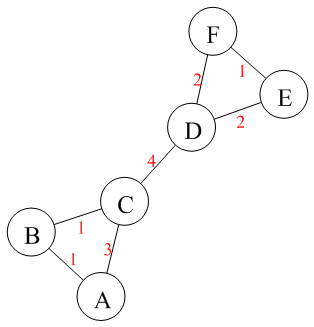
\includegraphics[height=8cm]{background/background-partitionhierarchies-pathfinding-transitiontable-a.png}}%
	%
	\hspace{4mm}%
	%
	\subfigure[]
	{
	\raisebox{1cm}{\begin{tabular}[b]{cc|cccccc}
	&& \multicolumn{6}{c}{Destination} \\
	&& A & B & C & D & E & F \\
	\hline
	\multirow{6}{*}{Source}
	& A  & $\times$ & B & B & B & B & B \\
	& B  & A & $\times$ & C & C & C & C \\
	& C  & B & B & $\times$ & D & D & D \\
	& D  & C & C & C & $\times$ & E & F \\
	& E  & D & D & D & D & $\times$ & F \\
	& F  & D & D & D & D & E & $\times$
	\end{tabular}}
	}%
\caption{A graph and its corresponding transition table -- each table entry $t_{SD}$ stores the node after $S$ on the optimal path between $S$ and $D$}
\label{fig:background-partitionhierarchies-pathfinding-transitiontable}
\end{stusubfig}
%---

Hierarchical pathfinding is an approach designed to reduce these prohibitive storage costs. The essence of the idea is to partition the graph into clusters. This partitioning of the graph into clusters creates a two-layer partition hierarchy (in this case a partition forest) of the graph nodes. Pathfinding schemes can then be devised that still produce optimal paths, but only store the substantially smaller transition tables for paths within each cluster and a transition table for an inter-cluster `super-graph' -- for an illustration of this sort of scheme, see Figure~\ref{fig:background-partitionhierarchies-pathfinding-kim}. The kind of storage savings that can be expected from this sort of approach are quantified by Dickheiser in \cite{dickheiser04}.

%---
\stufigex{height=11cm}{background/background-partitionhierarchies-pathfinding-kim.png}{Partitioning a large graph into clusters allows us to only store transition tables for each cluster (b) and the super-graph (c), rather than a transition table for the entire graph. When finding paths, all the necessary information is contained in the transition tables for the source cluster, the destination cluster and the super-graph (d). (The figure is reproduced from Kim et al.\ \cite{kim98}.)}{fig:background-partitionhierarchies-pathfinding-kim}{p}
%---

To find an optimal path between two nodes using this scheme, we observe that such a route can either (a) go from the source node to a boundary node of the source cluster, then (via the super-graph) to a boundary node of the destination cluster, then to the destination node, or (b) go directly from the source node to the destination node if they are in the same cluster. (Note that the shortest path between two nodes in the same cluster may actually go via the super-graph, so we have to consider both options in such a case.) An optimal intra-cluster route (where applicable) can simply be looked up in the cluster's transition table, but to find an optimal inter-cluster route is slightly more involved. To do so, we find three sets of optimal sub-paths:
%
\begin{enumerate}

\item $S = \{s_i\}$, the set of optimal paths from the source node to a boundary node of the source cluster. These can be looked up using the source cluster's transition table.
\item $P = \{p_j\}$, the set of optimal paths from a boundary node of the source cluster to a boundary node of the destination cluster. These can be looked up using the super-graph's transition table.
\item $D = \{d_k\}$, the set of optimal paths from a boundary node of the destination cluster to the boundary node. These can be looked up using the destination cluster's transition table.

\end{enumerate}
%
We then consider all possible paths $s_i \mbox{++} p_j \mbox{++} d_k$ (where $\mbox{++}$ represents path concatenation) and pick one with the lowest cost. This is minimised against any possible intra-cluster route where necessary to give a path that is optimal overall.

Thus far, we have only considered a pathfinding hierarchy with two layers, but the scheme can easily be extended to allow more layers if e.g.~the transition tables for the individual clusters are still considered too memory-intensive. The easiest way to do this is to treat each individual cluster as a graph in its own right and partition it into pieces (a top-down approach), although bottom-up approaches are also possible (one such approach, referred to in \cite{kim98}, can be found in \cite{jing96}). Actually constructing the partitions of individual graphs automatically is the problem known as graph partitioning or graph clustering (see e.g.~\cite{huang96,jing98}, or indeed \S\ref{subsec:graphpartitioning}). In certain domains (such as the computer games industry), the partitions may actually be constructed manually to gain finer control over the end result \cite{dickheiser04}. In either case, however, it is helpful to be able to edit the resulting partition forest interactively to try and minimise the amount of memory required to store the transition tables. This can be facilitated by the partition forest algorithms I will present in Chapter~\ref{chap:ipfs}.

\subsection{Team Organisation}

TODO

\subsection{World Representation}

TODO: \cite{finkel74,fuchs80}

%---
\section{Chapter Summary}

This chapter has given an overview of most of the techniques currently in use for medical image segmentation and provided some important background on the varied uses of partition hierarchies. In Chapter~\ref{chap:methodology}, I will discuss the design of my research in the context of these large bodies of existing work.

\chapter{Background}
\label{chap:background}

\emph{Draft Version}

%---
\section{Segmentation}

\subsection{Introduction}

Segmentation is a sub-field of image processing in which we try to partition an image into regions which correspond to interesting, or salient, features in the image. For instance, in medical image processing, we might try and segment a CT scan into regions which correspond to axial slices through major organs, e.g. the liver or a kidney. Segmentation is rarely useful on its own; rather, it tends to occur as a pre-processing step whose output (the partition of the image) is then used as input to later stages of an algorithm. An example usage is in the 3D visualization of organs, where the segmentation results for a series of slices can be used to identify which voxels in a volumetric dataset are contained within a given organ: a mesh can then be generated from this using any suitable algorithm from the visualization literature, e.g. \cite{cong05,lorensen87,wu03}.

Many different approaches are used to segment images. There is no `best' method which works well for every segmentation problem, so it is vital to select a method carefully based on the characteristics of the images under consideration. Since I will be dealing exclusively with \emph{medical} image segmentation of abdominal scans for the purposes of my thesis, I will only discuss techniques applicable in that domain in this review, but even with that restriction in place, there are several different image modalities (e.g. CT, MRI, US) which may be encountered and a large number of different segmentation methods in use \cite{pham00,varshney02}.

Each segmentation algorithm has its own characteristics (e.g. resilience to noise, connectedness of output, etc.), making it more or less suitable for a given problem. Some algorithms output region boundaries (contours) rather than an actual partition of the image \cite{kass88,lobregt95,xu98}: this may or may not be desirable in a given context (although it is worth noting that is often possible to subsequently convert between region-based and boundary-based representations). Furthermore, the degree of automation of the algorithms varies. At one end of the spectrum, images can be manually segmented by a radiologist: this generally gives excellent results (although they may not necessarily be entirely consistent between different radiologists) but requires more human interaction, although radiologists have got this down to a fine art. At the other extreme, we can try and develop algorithms which segment images automatically \cite{lee03, lin06, marcotegui05, meijster98, park03, soler01, touhami05, tsagaan02}: these reduce the burden on the human user, but it is rare that results are attained which are comparable with those which can be produced manually, not least because radiologists sometimes have to rely on anatomically-informed judgement to decide where the boundary of an object of interest lies and it is difficult to incorporate this expert knowledge into a computer program. That being said, some teams have achieved exceptionally good results in this area. Of particular note is the work done by Luc Soler's team in France \cite{soler01} which aims to delineate anatomical structures relevant to hepatic surgery. Clinical validation on over 30 patients has shown that their fully-automatic segmentation technique on 2mm-thick enhanced spiral abdominal CT scans generates results which are often actually \emph{better} than the manual segmentation produced by a radiologist.

In general, though, some degree of interactivity in segmentation procedures currently remains desirable, whether this merely involves allowing a radiologist to make adjustments to the output, or actually involves requesting user input to the algorithm itself (for example, a region growing algorithm might require seed points). There is a lot of overlap between the methods used for fully-automatic and semi-automatic segmentation --- in general, fully-automatic segmentation tends to focus (not surprisingly) on automating the difficult-to-automate aspects of semi-automatic algorithms --- so I will review approaches from both sub-fields in the following sections.

\subsection{Thresholding}

%TODO: \cite{kobashi95,seo05}

%In principle, thresholding segmentation methods are quite simple. The idea is to divide the pixels of the image into two (in the case of binary thresholding) or more (in the case of multithresholding) classes through the use of one or more dividing lines on the image histogram. For example, in an 8-bit image where the grey levels ranged from 0 (black) to 255 (white), we could decide that all pixels whose grey value was greater than 160 (say) represented the foreground of the image, and all other pixels represented the background.

In principle, thresholding segmentation methods are quite simple. The idea is to divide the pixels of the image into classes through the use of one or more dividing lines on the image histogram. Dividing the image into two classes is known as \emph{binary thresholding}; where more classes are used, we refer to the process as \emph{multi-thresholding}. As an example, we could use binary thresholding to divide an 8-bit image (with grey levels ranging from 0=black to 255=white) into two classes, one containing pixels greater than (say) 160, and representing the foreground of the image, and the other containing all the remaining pixels and representing the background.

The difficulty encountered in practice is how to determine the optimum threshold location(s). A misplaced threshold will cause an inaccurate segmentation, so choosing the location appropriately is essential. In our example above, choosing a threshold which was too high would mean that the foreground of the image would be \emph{undersegmented} (i.e. pixels which should be classified as being part of the foreground are incorrectly classified as background) and the background would be \emph{oversegmented} (the converse). Choosing too low a threshold would cause the opposite problem.

Owing to difficulties like this, applications are often designed so that thresholds can be chosen interactively by the user, but a great deal of work has also been done on automatically determining good threshold locations. As surveyed in \cite{sezgin04}, there are six types of approach to the problem in current use, including:

\begin{enumerate}

\item \emph{Histogram shape-based methods.} These use shape properties of the histogram to find a good threshold. For instance, Rosenfeld's histogram concavity method, cited in \cite{lee.c92}, works by examining the difference between a histogram and its convex hull. A grey level at which the the height difference between the histogram and its convex hull is greatest (i.e. a point of deepest concavity) is picked as the threshold value.

\item \emph{Clustering-based methods.} These try and group the grey level data into a given number of clusters (two in the case of binary thresholding). One example is the method of Ridler and Calvard \cite{ridler78}. Their idea was to take a grey-level image and produce an initial binary classification which makes the assumption that the object of interest is somewhere in the middle of the image and the corners of the image contain only background. The means of the pixels currently classified as background and object are calculated and the average of the two means is taken. The new value is then used to threshold the image and produce a new binary classification into background and object classes: it is assumed that this will be more accurate than the initial guess. Finally, the process is iterated until there is little or no change in the binary classification, and the last threshold in the iteration is chosen for use.

\item \emph{Entropy-based methods.} These are based on information theory and pick thresholds by (for example) trying to maximise the information content in the thresholded image. As described in \cite{wong89}, the simplest possible method looks at two probabilities, $F(T)$ and $F^*(T) = 1 - F(T)$, each parameterised in terms of a threshold, $T$. The first, $F(T)$, gives us the probability of a given pixel having a grey value less than or equal to the threshold, and the second, $F^*(T)$, gives us the probability of the value being greater than it. The information content in the thresholded image is given by
%
\[
H(T) = -F(T) \log_2 F(T) - F^*(T) \log_2 F^*(T)
\]
%
and attains a maximum when $F(T) = 0.5$. This is equivalent to saying that in the absence of any other knowledge, the maximum entropy principle tells us that the information contained in the thresholded image is maximised by picking a threshold which classifies half the pixels as background and half as foreground. This makes intuitive sense, but is too simplistic an approach for the majority of applications. Better alternatives have been developed, but are beyond the scope of this report.

%\item \emph{Object attribute-based methods.}

%\item \emph{Spatial methods.}

%\item \emph{Local / adaptive methods.}

\end{enumerate}

\noindent In spite of the large amount of work done on thresholding, however, it has some significant downsides when used on its own to process medical images:

\begin{itemize}

\item It divides the image into two or more groups of pixels, based on their grey values, but there is no guarantee (or even an expectation) that any of these groups will be contiguous in the image. For instance, trying to segment a kidney from a CT scan by bounding it between two grey value thresholds might also result in inadvertently segmenting blood vessels across the image as well (their grey levels are quite similar to those of the kidneys). Not only are these blood vessels not part of the kidney, they are actually physically separated from it in the image! (It is also worth noting that trying to segment a kidney will generally result in segmenting both of them at once, since their grey level ranges are the same. This sort of problem can be overcome by specifying the side of the body in which we're interested.)

\item It is by no means the case that acceptable threshold locations always exist. If the grey value ranges of different objects of interest significantly overlap, it may be impossible to separate them using thresholding alone.

\end{itemize}

%For reasons like this, I believe that thresholding is not the most appropriate choice of method for my work. However, I have found a use for it when trying to quantify the extent of necrosis in a tumour (see Chapter~\ref{chapter:existingwork}).% Whilst it is true that thresholding can be made to produce reasonable results (e.g. \cite{kobashi95}), I feel that there are other algorithms which

These limitations can often be overcome by combining thresholding with other techniques. For instance, the results of thresholding often have gaps in them, which can sometimes be filled in by carefully applying various morphological operators (e.g. morphological opening and closing). Luc Soler's team \cite{soler01} made use of thresholding (as one technique among many) and achieved excellent automatic segmentation results for the liver. However, they did not use thresholding on its own. For instance, they segmented bones by thresholding for bright areas and then keeping only those which were near to the fat tissue (which had already been segmented). Simple thresholding alone would have been insufficient for the task, since structures such as the aorta also appeared bright on the contrast-enhanced images.

%Whilst thresholding has its limitations, it has been nevertheless been successfully incorporated into more general segmentation algorithms, sometimes with spectacularly good results. The work of Luc Soler's team \cite{soler01}, as previously commented on, is particularly noteworthy in this regard. One example of how they use thresholding to achieve good results is when they are segmenting bones. A simple thresholding operation would fail, since the contrast agent used when the scans were taken causes structures such as the aorta to appear bright. Instead, they isolate the fat tissue and define the bones as being bright structures close to that. They also post-process their thresholding operations with morphological operators to fill in any unwanted gaps.

\subsection{Region Growing}

%TODO: \cite{lin06,pohle01}

Region growing methods for segmentation essentially work as follows. First, an initial seed point is chosen for a feature of interest. Then, the region is `grown' by iteratively considering all points which are adjacent to the region and adding any which satisfy certain criteria. For example, we could choose to add adjacent pixels whose grey value differs from that of their neighbour in the region by less than a certain amount. Alternatively, we could try and add adjacent pixels which preserve the homogeneity of the entire region (for some suitable definition of homogeneity). A basic region growing algorithm can be implemented straightforwardly using a queue. Starting from a queue containing only the initial seed point, we repeatedly pop the pixel at the front of the queue, consider its non-region neighbours for addition to the region, and push any which satisfy the requisite criteria onto the end of the queue. The process terminates when the queue empties.

The key issues when implementing region growing are how to choose the seed point, how to formulate the criteria specifying which points to add to the region, and how to decide when the process should terminate. For automated segmentation methods, how to choose the seed point is of fundamental importance; semi-automated algorithms can focus exclusively on the latter two problems, relying instead on the user to interactively specify an initial seed.

As mentioned above, one of the simplest approaches to region growing is to add adjacent pixels which are within a certain fixed threshold value of their neighbour in the region. Practical region growing methods, however, such as \cite{lin06,pohle01}, tend instead to use \emph{adaptive} region growing, whereby the criterion varies to take account of the area around the pixel under consideration. In \cite{lin06}, for example, the approach taken is as follows. After locating an initial seed point $(s_x, s_y)$, a $7 \times 7$ mesh is placed over it and the maximum and minimum pixel intensities within the mesh, $M(s_x, s_y)$ and $m(s_x, s_y)$ are determined. From these, a contrast range $t_0 = M(s_x, s_y) - m(s_x, s_y)$ is calculated and recorded. Next, for each pixel $(x,y)$ under consideration for addition to the region, values $M(x,y)$ and $m(x,y)$ are similarly calculated, and a local value $\theta_{\rm local} = (M(x,y) + m(x,y)) / 2$ is determined. The region growing criterion is then formulated as $|f(x,y) - \theta_{\rm local}| \le t_0$, i.e. we add an adjacent pixel $(x,y)$ to the region if the absolute difference between its grey value $f(x,y)$ and the midpoint of the contrast range of the $7 \times 7$ mesh surrounding it is less than the contrast range of the $7 \times 7$ mesh centred on the initial seed point. The region growing is specified to stop when this absolute difference is greater than a certain threshold, implying that the area surrounding a given pixel is not homogeneous.

The advantages of region growing methods are that the resultant region is guaranteed to be connected in the image (unlike with thresholding) and that they are, on the whole, fairly easy to implement. However, from the point of view of automatic segmentation, they present difficulties, because choosing an initial seed point is in general a non-trivial problem. The usual approach taken for automatic seed point selection is to rely on statistical data about where the features of interest (e.g. organs) usually lie in the body. For instance, the approach in \cite{lin06} is to search for suitable seed points in two elliptical regions on each side of the body, one for each kidney. This works quite well, but doesn't seem as if it would be that robust if tested on unusual cases.

Whilst region growing algorithms are guaranteed to produce a connected result, the region may still have holes in the middle of it. Whilst this may be desirable if we really are trying to segment a torus-shaped feature, on the whole we need to post-process the region growing results to remove these holes. Common techniques for doing this include morphological closing, etc.

\subsection{Approaches from Mathematical Morphology}

In the words of some of its practitioners\footnotemark{}, the field of mathematical morphology espouses a `non-linear approach to image processing'. Its interesting techniques include dilation, erosion, and morphological opening and closing, but our emphasis in this report will be on one particularly useful morphological technique for image segmentation: the watershed transform.

\footnotetext{The Centre for Mathematical Morphology at the Ecole des Mines de Paris.}

\subsubsection*{The Watershed Transform: Techniques}

%TODO: \cite{bieniek00,meijster98,osma-ruiz06,rambabu07,stoev00}

\emph{Note: I have written an article on the watershed transform for ACCU's Overload journal, which appears as Appendix~\ref{chapter:watershed} in this report. For that reason, I plan to give only a limited presentation of the technique here. Readers are referred to the appendix for more information.}

The idea of the watershed transform is to view an image as a landscape and divide it up into valleys. Each valley in the landscape will correspond to a region in the segmentation result. We don't perform the transform on the actual image to be segmented, since its valleys may not correspond to the features we're interested in. Instead, we take the initial image and try and generate a derived image from it in which the valleys correspond to our features of interest: in the case of medical images, this often involves something similar to taking the gradient of the initial image, since organs tend to look fairly homogeneous on scans (and thus the magnitude of the gradient within them is low). The derived image then becomes the input to the watershed transform itself.

In terms of implementation, the watershed transform can be viewed in one of two different ways:

\begin{enumerate}

\item \emph{A flooding/immersion process}. Imagine poking holes in the local minima of the landscape and then lowering the landscape vertically into a lake. As the landscape is lowered, water will seep through the holes and catchment basins will form in each of the valleys of the image. As the water continues to rise, some of the catchment basins will meet: at this point, we add dams, or watersheds, to keep them apart, and continue lowering the landscape. At the end of the process, the dams we added will act as dividing lines between the valleys, thus segmenting the underlying image into regions.

\item \emph{A rainfall process}. Imagine dropping a raindrop at each point in the landscape. Assuming the image has no (non-minimal) plateaux (flat regions), the drop will run downhill, via a path of steepest descent, until it ends up in a local minimum. (There are ways of dealing with non-minimal plateaux, e.g. the method described in the appendix.) The point at which it started will be associated with this local minimum (it will be called part of the minimum's catchment basin) and the process will continue until all the points in the landscape have been processed. The result will be a region-based partition of the landscape (and hence the underlying image) into catchment basins, one per local minimum.

\end{enumerate}

These two alternative ways of viewing the process have led to two different classes of techniques. In particular, \cite{bieniek00} and \cite{rambabu07} are examples of the former approach, and examples of the latter can be found in \cite{meijster98,osma-ruiz06,stoev00}. It is worth noting that the various definitions are not always exactly equivalent. For example, some approaches generate results containing watershed lines, whilst others generate only regions. Also, rainfalling approaches don't generally give identical results to their immersion-based counterparts. It is thus important to choose an appropriate method with care.

\subsubsection*{The Watershed Transform: Pre-Processing}

%TODO: \cite{ancin95}

The biggest problem with the watershed transform as a segmentation approach is that it is overly affected by spurious local minima in the landscape. This leads to massive over-segmentation of the image. To explain the problem, consider an analogy. If we try and divide a dimpled landscape into valleys, counting each dimple (small hollow) in the landscape as a valley, then we will end up with vast numbers of `irrelevant' valleys at the end of the process, obscuring the more significant valleys we are trying to find: this is essentially the problem faced by the watershed transform. The `dimples' in an image can be caused by things like noise, but even in the absence of image artifacts, there will usually be valleys corresponding to features in which we have no interest. We need a way of separating the wheat from the chaff.

To overcome this difficulty, various approaches have been suggested in the literature. The effects of less prominent noise can be mitigated to an extent by smoothing the image, although care must be taken not to blur the edges in the image when doing this. Another approach \cite{ancin95} is to suppress some of the irrelevant contours in the gradient image by determining the connected components of the gradient image and removing (by setting the pixels of the component to zero) all those whose size is less than a threshold (e.g. the perimeter of the smallest object of interest).

One technique which works quite well in practice is to apply spatially-variant smoothing to the image: instead of smoothing uniformly over the entire image, the idea is to smooth less in areas where we think there may be edges. This is the idea behind non-linear diffusion filters \cite{perona90}. (In Chapter~\ref{chapter:existingwork}, I describe another approach based on similar principles.)

\subsubsection*{The Watershed Transform: Post-Processing}

%TODO: \cite{beucher01,patino05,marcotegui05,wegner95}, \cite{najman96} (mention correction paper)

The approaches described so far try to pre-process an image (or its gradient image) to reduce watershed over-segmentation. Post-processing the watershed results is also possible, and in general a combination of both techniques tends to be employed.

The general idea of watershed post-processing is to try and merge the large number of generated regions together in a way that generates larger regions corresponding to our objects of interest. Attempts can be made to group together similar regions using fuzzy relations, e.g. \cite{patino05}.

The idea of region-merging can also be used to create partition hierarchies, intuitively corresponding to a series of segmentations of an image at different scales. For example, the waterfall algorithm \cite{beucher01,marcotegui05} merges regions by iteratively running a watershed-from-markers algorithm on the region adjacency graph of the watershed result. (Note that I have described it in much more detail in Appendix~\ref{chapter:waterfall}.) This is particularly useful when trying to pick out organs of different sizes. A similar approach is described in \cite{wegner95}.

The type of hierarchy generated by the waterfall algorithm is by no means the only possible hierarchy, and indeed it may converge (to a single region) too fast for some applications. Alternative hierarchies are also possible, e.g. ones based on the saliency of contours in the watershed results \cite{najman96}.\footnotemark{}

\footnotetext{Whilst this is generally a good paper, it is worth noting that it contained an error which had to be corrected later in a comment \cite{lemarechal98}. An improved correction was then published by one of the original authors \cite{schmitt98}. All three should be read together to avoid confusion.}

%\subsubsection*{The Watershed Transform: Applications}

%TODO: \cite{bueno01,grau04}, mention \cite{najman95} in the context of registration

\subsection{Deformable Models}

%Model fitting methods, as their name suggests, attempt to fit a model of the features under consideration to the actual data available. They essentially make use of \emph{a priori} anatomical knowledge at an early stage of the segmentation process to improve the generated results. The actual model used can take a variety of different forms, ranging from deformable models, whereby the model is represented explicitly (perhaps as a contour on the image), to implicit model representations such as probabilistic atlases and neural networks. I will briefly survey each of these methods in the subsections which follow.

%As their name suggests, deformable models methods work by taking an initial model of the features under consideration and deforming it to fit the actual data available. The initialisation of the model is generally based on \emph{a priori} anatomical knowledge. As observed in \cite{suri02}, there are two basic types of deformable model, namely \emph{parametric} and \emph{geometric}. Geometric deformable models have been developed more recently than their parametric counterparts, but both types see a lot of use. The most well-known examples of the two types are snakes and level sets, which will be discussed in detail in the following two subsections.

As their name suggests, deformable models methods work by taking an initial model of the features under consideration and deforming it to fit the actual data available. The initialisation of the model is generally based on \emph{a priori} anatomical knowledge. The model itself can be represented in a variety of ways, and these ways correspond to a number of different approaches to the problem. For example, the snakes method, which we will see shortly, represents the model as a parametrically-defined spline, and is hence referred to as an example of a parametric deformable model (it is sometimes also referred to as an explicit deformable model). In contrast, level sets represent the model \emph{implicitly} and are an example of implicit deformable models. Implicit deformable models were developed more recently than their parametric counterparts, but both types see a lot of use.

\subsubsection{Snakes}

%TODO: \cite{cohen91,kass88,lobregt95,xu98}

As originally defined by Kass, Witkin and Terzopoulos in \cite{kass88}, ``A snake is an energy-minimizing spline guided by external constraint forces and influenced by image forces that pull it toward features such as lines and edges.''

Essentially, the idea works as follows. We represent the position of the snake, in terms of a spline parameter $s$, as $\mathbf{v}(s) = (x(s),y(s))$, and define an \emph{energy functional}, $E_{snake}^*$, as
%
\[
E_{snake}^* = \int_0^1 E_{int}(\mathbf{v}(s)) + E_{image}(\mathbf{v}(s)) + E_{con}(\mathbf{v}(s)) \; ds.
\]
%
The three terms in the summation are \emph{internal} energy, which tries to limit the curvature of the snake, \emph{image} energy, which tries to attract the snake towards features in the image such as lines and edges, and \emph{constraint} energy, which allows the user to apply constraints to influence the result of the segmentation. The snake algorithm as a whole attempts to find a spline minimising $E_{snake}^*$.

The original snakes paper describes a continuous model, but more recent research \cite{lobregt95,miller90b,miller90a} has seen the development of discrete models as well. The model described by Lobregt and Viergever in \cite{lobregt95}, called a \emph{discrete dynamic contour model}, is particularly interesting, both because it is intuitively easy to understand, and because it links in with my previous work. It is thus worth describing in more detail.

Rather than relying on ideas of energy-minimization, Lobregt and Viergever model snakes using a force-based physical simulation (note that this ties in well with my earlier work on physical simulations of long hair \cite{gvc08}). In their approach, a snake is a set of vertices connected by edges. At each time-step, various forces are applied to each vertex, which gradually \emph{deform} the snake towards the desired result. The results of this approach will depend to an extent on the lengths of the edges joining the vertices: if an edge is too long, important image features may pass through the gaps between vertices; if it is too short, the snake may become overly fixated on small details, not to mention the speed of the process being adversely affected. For this reason, after each deformation step, the snake is \emph{resampled} (by adding or removing vertices where necessary) to keep the edge lengths within certain limits.

The forces applied to each vertex closely mimic the energy terms in the original snakes paper. The force $\mathbf{f_i}$ applied to vertex $i$ is defined as the weighted sum
%
\[
\mathbf{f_i} = w_{ex}\mathbf{f_{ex,r_i}} + w_{in}\mathbf{f_{in,i}} + \underbrace{w_{damp}}_{< \; 0}\mathbf{v_i},
\]
%
where $\mathbf{f_{ex,r_i}}$ is an \emph{external} force term corresponding to the image and constraint terms from the original formulation, $\mathbf{f_{in,i}}$ is an \emph{internal} force term corresponding to the original internal term, and the remaining term is a new addition used to apply damping to try and bring the simulation to rest. (The real numbers $w_{ex}$, $w_{in}$ and $w_{damp}$ specify the weights to be given to each of these three factors. The paper tended to set all three of these to $0.5$: apparently this was derived empirically.)

It is important to mention that the method relies on quite a close initialisation (i.e.\ image features have quite a short capture range). In \cite{ree05}, this problem is circumvented by peforming a watershed-from-markers segmentation and using the result of that to initialise the snake. Another alternative, referred to there, is to try and add additional external forces to solve the problem: in particular, some success has been had with \emph{balloon forces} \cite{cohen91} and \emph{gradient vector flow} \cite{xu98}.

Problems of this kind with snakes methods have led to a great deal of interest in level sets as an alternative, although snakes also remain popular as a well-established and far simpler alternative. They also have the advantage that they can represent open structures as well as closed ones.

\subsubsection{Level Sets}

%TODO: \cite{sorlie05}

Level sets are to snakes what implicit representations of functions are to parametric ones. As an initial introduction, consider the alternative representations of a circle of radius $r$, centred at the origin. An implicit representation could be
%
\[
x^2 + y^2 = r^2,
\]
%
whereas a parametric representation in terms of an angle $\theta$ could be
%
\begin{eqnarray*}
x & = & \cos \theta \\
y & = & \sin \theta.
\end{eqnarray*}
%
Now, consider a more general form of the above. Instead of thinking about circles, consider the function $\phi(x,y) = x^2 + y^2$, which defines a scalar field over $\mathbb{R}^2$. For any value $k > 0$, the equation $\phi(x,y) = k$ defines a circle in the x-y plane: we will refer to each of these circles as an \emph{isosurface} of $\phi$, because each of them is the surface (curve) of all the points at which $\phi$ takes a particular value\footnotemark{}.

\footnotetext{\emph{Iso} means `equal' in Greek, so here we are talking about the surface containing all the points with the same $\phi$ value.}

Note what happens if we change $\phi$. If we redefine it as $\phi(x,y) = x^3 + y^3$, the isosurfaces change from being circles to hypercircles. This is a key idea: by changing the function $\phi$, we can move the isosurfaces of $\phi$ around, \emph{without having to represent them explicitly}. This is the insight behind level sets: we represent the contour we're interested in as an isosurface of some function $\phi$, then modify $\phi$ to modify the contour. Instead of using simple functions like $x^2 + y^2$ for our $\phi$, we can think of a general function $\phi: U \to \mathbb{R}$, where $U \subset \mathbb{R}^2$.

In practice, to represent contour changes over time, we make $\phi$ a function of time as well, giving us $\phi(\mathbf{x},t): U \times \mathbb{R}^+ \to \mathbb{R}$. We then set this equal to some constant $k$ to actually specify which isosurface of $\phi$ we're interested in.

Consider a simple example, that of a circle, centred at the origin, which gradually expands outwards as the time increases (see Figure~\ref{fig:levelsets-circle}).

%---
\stufigex{height=7cm}{background/levelsets-circle.png}{A simple circular contour which gradually expands over time}{fig:levelsets-circle}{H}
%---

In particular, suppose its radius is $t$ at time $t$. We represent this as:
%
\[
\phi((x,y), t) = \frac{x^2 + y^2}{t^2} = 1 = k
\]
%

For a more complicated example, consider gradually changing the circle into an ellipse over time (see Figure~\ref{fig:levelsets-ellipse}).

%---
\stufigex{height=7cm}{background/levelsets-ellipse.png}{An example of a contour which changes its shape over time}{fig:levelsets-ellipse}{H}
%---

This could be achieved by writing the following:
%
\[
\phi((x,y), t) = \left(\frac{x}{t}\right)^2 + y^2 = 1 = k
\]
%

In practice, we are almost never able to give an explicit function for $\phi$: the simple examples above notwithstanding, it's just not possible for real-world applications. Instead, we discretise the process by specifying initial values for $\phi$ at points on a discrete grid, then derive a partial differential equation for $\phi$ and solve it numerically to modify the contour over time. The PDE in question can be found by taking the total derivative of
%
\[
\phi(\mathbf{x}, t) = k,
\]
%
giving us
%
\[
\pd{\phi}{t} = -\nabla\phi \cdot \mathbf{v},
\]
%
where $\mathbf{v} = \pdnf{\mathbf{x}}{t}$. By making $\mathbf{v}$ a function of the position of $\mathbf{x}$ and the geometry of the surface (which it turns out can be represented by the differential structure of $\phi$), we can control how we want the contour to evolve over time.

How to numerically solve the above equation is beyond the scope of this report, but before moving on, I would like to look at a concrete example of the method on a discrete grid, to illustrate some of its advantages. Consider the discrete grid of $\phi$ values in Figure~\ref{fig:levelsets-discrete1}(a). The marked points form an isosurface of $\phi$, specifically the $k = 4$ isosurface. This is entirely analogous to the examples above, but on a discrete grid instead of in a continous space. By changing the grid values, as in Figure~\ref{fig:levelsets-discrete1}(b), we can move the isosurface however we wish.

%---
\begin{figure}[H]
\begin{center}
	\subfigure[]{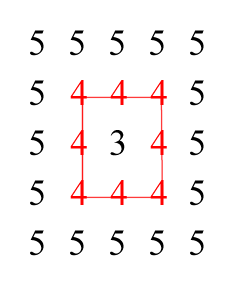
\includegraphics[height=5cm]{background/levelsets-discrete1a.png}}%
	\hspace{4mm}%
	\subfigure[]{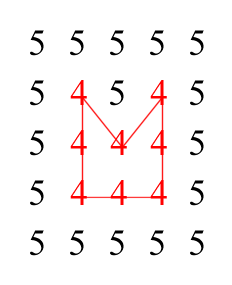
\includegraphics[height=5cm]{background/levelsets-discrete1b.png}}
\end{center}
\caption{An example of level sets on a discrete grid}
\label{fig:levelsets-discrete1}
\end{figure}
%---

Now, consider the further example shown in Figure~\ref{fig:levelsets-discrete2}(a). Here the situation seems more complicated, in that the points on the $k = 4$ isosurface are not all connected to each other. This is actually an advantage of the level set method, however. By representing the surface implicitly, we can model surfaces with multiple connected components without having to do any additional work. Indeed, the number of components can evolve over time: in Figure~\ref{fig:levelsets-discrete2}(b), we see that the two components can be joined by simply changing the value of $\phi$ at one of the grid points to $5$.

%---
\begin{figure}[H]
\begin{center}
	\subfigure[]{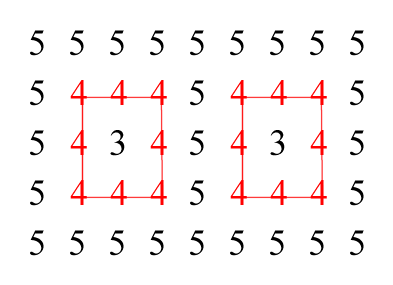
\includegraphics[height=5cm]{background/levelsets-discrete2a.png}}%
	\hspace{4mm}%
	\subfigure[]{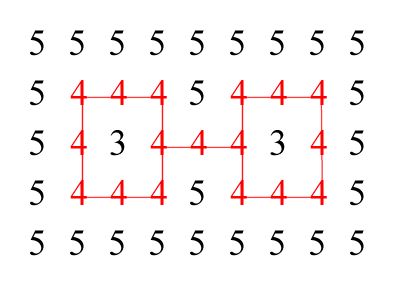
\includegraphics[height=5cm]{background/levelsets-discrete2b.png}}
\end{center}
\caption{An example with more than one connected component}
\label{fig:levelsets-discrete2}
\end{figure}
%---

One final advantage of level sets worth mentioning is that the method works equally well in 3D, although the extra processing involved means that clever numerical techniques are required. The details of how these work are beyond the scope of this report but, as an example, one method (the narrow-band technique) basically restricts numerical calculations to a narrow region around the isosurface we're particularly interested in. The insight is that solving the PDE over the whole domain is only necessary if we're interested in solving for the entire family of isosurfaces associated with $\phi$: often we're only looking at a single isosurface, so the extra computations aren't necessary. For more details, take a look at \cite{yoo04}.

\subsubsection{Other Deformable Models}

%TODO: \cite{jalba04,rao05,tsagaan02}

Other notable parametric deformable models in existence include the contribution of Tsagaan et al. \cite{tsagaan02}, who used a NURBS-based model of a kidney and deformed it by minimising an energy function. Their results seem good in some cases, but differ markedly from the manually segmented results in others.

Parametric and implicit models are not the only types of deformable model in use, however. In particular, \cite{jalba04} uses a deformable model based on charged particles to achieve some interesting automatic segmentation results. Here, the model is represented as a set of charged particles under the influence of an electrostatic field. The authors' work in this area is still ongoing. Yet another deformable model can be found in \cite{pizer03}, in which the authors' make use of a medial representation known as m-reps.

\subsection{Learning Methods}

Learning segmentation methods generally start with a training phase, in which a large number of scans are taken and used to construct some variety of model, which encodes information that can be used to segment subsequent scans. Two different types of learning method will be discussed in the following subsections.

\subsubsection{Atlas-Based Approaches}

%TODO: \cite{park03,zhou05}

Atlas-based methods start by constructing an atlas, or reference segmentation, from a set of training data. For instance, in \cite{park03}, a probabilistic atlas was constructed by registering (aligning) the manually segmented volumes of 31 patients onto that of a carefully chosen reference patient (thus the data came from 32 patients in all). The atlas was represented as a 3D grid of vector values, where the components of each vector corresponded to the organs under consideration, and the values of the components indicated the fractional percentage of registered data sets in which the point was labelled as the given organ. As an example, if we were considering the liver and the two kidneys, the vector $(0.4, 0.6, 0)^T$ at a point could indicate that the point was inside the liver in 40\% of the data sets and inside the right kidney in 60\% of them.

After constructing such an atlas, new sets of data can be segmented by registering them onto it. In \cite{park03}, they use a \emph{maximum a posteriori} (MAP) approach after registration to find the segmentation result which best explains the observed data. The important point here is that the segmentation result is based on both the data for the individual patient and the information encoded in the atlas. The atlas provides the prior probabilities at each voxel, and these are refined in light of the actual patient data.

To use the notation in \cite{park03}, we denote the segmentation result field as $\mathbf{X}$, the field of observed data for the individual patient as $\mathbf{Y}$, and the probabilistic atlas as $\mathbf{A}$. Each of these represents a volume of $N$ voxels, indexed linearly (in some order) from $1$ to $N$. So for instance, a particular segmentation result could be given by $\mathbf{x} = (x_1, x_2, \ldots, x_N)$. Our aim is to find the best possible $\mathbf{x}$, defined as
%
\[
\mathbf{\hat{x}} = \argmax_{\mathbf{x}} \mathbf{P}(\mathbf{X} = \mathbf{x} | \mathbf{Y} = \mathbf{y}).
\]
%
In other words, we seek the segmentation result which best explains the observed patient data, $\mathbf{y}$. The probabilistic atlas is used in all of this as the prior for $\mathbf{X}$. Suppose there are $L$ different possible voxel labels, numbered from $1$ to $L$. Each voxel $a_i$ of the probabilistic atlas contains an $L$-vector, $(a_{i,1}, \ldots, a_{i,L})$, where $a_{i,\ell}$ gives the probability of a voxel's correct label being $\ell$. We use this to define the prior probabilities for $\mathbf{X}$, writing
%
\[
P(x_i = \ell) = a_{i,\ell}.
\]
%
In other words, the probability of the correct segmentation result for a given voxel being $\ell$ is given by the $\ell^{th}$ component of the probabilistic atlas at that location. With this link made, the result determined will depend on both the atlas and the observed data.

\subsubsection{Neural Network Methods}

%TODO: \cite{lee03,tsai94}

Neural networks (NNs) can be used to segment images in a number of ways. A simple NN technique can be found in \cite{tsai94}, where the authors use a feed-forward network to classify each pixel into one of three classes (liver, boundary or non-liver) according to the grey-level histogram of the 7x7 region centred on the pixel. (In practice, they use a histogram with 16 grey levels instead of 256, to avoid a proliferation of input nodes in the NN.) The schematic of how this works (borrowed from their paper) is shown in Figure~\ref{fig:neuralnets-tsai}.

The NN is initially trained by picking a suitable image from the middle of the volume and marking a significant number of training regions for each class. The well-known back-propagation algorithm for NNs is used to update the weights on the network arcs accordingly.

The results of the scheme are somewhat hard to evaluate since the images in this somewhat old paper (1994) have not really survived the ravages of time. However, they do seem to show that the authors have obtained something that looks reasonably like a liver, so the method has some merit.

%---
\stufigex{height=20cm}{background/neuralnets-tsai.png}{Schematic diagram of the neural-network-based boundary detection method used in \cite{tsai94} (borrowed from the paper in question)}{fig:neuralnets-tsai}{H}
%---

\clearpage

A more up-to-date (and more complicated) NN scheme can be found in \cite{lee03}. Here, the authors use a multi-module, recurrent neural network to segment multiple abdominal organs (see Figure~\ref{fig:neuralnets-lee}). There is a module associated with each label under consideration. Each node of a given module $k$ corresponds to a pixel in the image and encodes the probability that the pixel should be assigned label $k$. The weights of the network arcs are initially derived from (for example) a correlation matrix containing the likelihoods of various labels occurring next to each other. (For example, the liver might be quite likely to occur next to the right kidney, but definitely shouldn't occur next to the left kidney.) An iterative state evolution algorithm is used to determine the probabilities at each node in each of the modules of the NN. The initial probabilities are generated using something called the `Kohonen self-organizing algorithm' (see the paper for details) and the nodes are updated at each time step based on the current probability at a given node and the support it receives from its neighbours. (So, for instance, if a pixel was currently classified as part of the left kidney, but all its neighbours were liver, it would be very likely to change to liver over time.) The results of this method (after combining it with fuzzy spatial rules for organ identification) are quite good (though the authors admit that more work is needed).

%---
\stufigex{height=8cm}{background/neuralnets-lee.png}{The architecture of the contextual neural network used in \cite{lee03} (borrowed from the paper in question)}{fig:neuralnets-lee}{ht}
%---

%\subsubsection{Statistical Methods}

%TODO: \cite{touhami05}

\subsection{Hybrid Methods}

%TODO: \cite{soler01}

It is often possible to achieve better results by combining a number of different segmentation methods than it is by using a single method on its own. A striking example of how successful this sort of technique can be is the work of Luc Soler's team in Strasbourg \cite{soler01} (see Figure~\ref{fig:soler} for a screenshot from their surgical tool).

%---
\stufigex{width=12cm}{background/soler.png}{An automatic 3D reconstruction of patients from medical images, as performed by the IRCAD surgical planning tools}{fig:soler}{t}
%---

The cited paper represents only a small part of their work on a surgical tool, and focuses on automatically segmenting the liver. Their segmentation method first uses thresholding, morphological operators and distance maps to identify the skin, bones, lungs, kidneys and spleen. The second stage is then effectively a clever deformable model approach in which they embed a reference model of the liver into the image and automatically deform it to the liver contours. Later stages use Gaussian fitting on the image histogram to separate normal liver tissue from blood vessels and lesions (tumours), a result which is further refined by their own analytical methods. The final stage of their work makes use of higher-level medical knowledge to label the hepatic portal vein and segment the liver anatomically: these features are not visible from the scans alone. As the screenshot shows, the results of this extensively hybrid technique are excellent.

Another couple of hybrid segmentation methods can be found in \cite{imielinska04}, in which the authors combine fuzzy connectedness, Voronoi diagram classification and deformable models into one segmentation method, and Gibbs priors and deformable models into another. The details of these techniques are beyond the scope of this report, but an implementation of the methods can be found in the popular (and freely-available) \emph{Insight Toolkit}.

\subsection{Evaluation of Segmentation Results}

%TODO: \cite{zhang96}

In many ways, evaluating the results of a segmentation process is just as important as segmenting the image in the first place. As described in \cite{zhang96}, there are essentially three different types of evaluation method in common use: analytical methods, empirical goodness methods and empirical discrepancy methods.

\emph{Analytical methods} deal with the actual algorithms rather than their results: they focus on things like the complexity of the algorithm, or its requirements. They usually produce qualitative results that are not directly tied to the segmentation accuracy for particular applications, which is often what we really want to know.

\emph{Empirical goodness} methods evaluate the segmentation results in terms of subjectively-defined `goodness' measures. For instance, some researchers have proposed methods which rate the results on their levels of intra-region uniformity (with high uniformity more desirable) and inter-region contrast (with high contrast more desirable). The advantage of using a method like this is that it can be applied directly to the segmentation results, without reference to any external source of information like a `gold standard' segmentation result. The disadvantage is that methods like this provide only subjective measures of segmentation quality.

In contrast, \emph{empirical discrepancy} methods compare the segmentation results to a `gold standard' result. This has the disadvantage of requiring us to have such a reference result (in the case of medical images, we may have to ask the radiologist to manually segment an image for us), but gives us a reasonably objective, quantitative evaluation of our algorithm in the context of a given application. One simple method in this category is to calculate the percentage of pixels misclassified. More complicated methods are also possible.

%---
\section{Region Classification / Organ Identification}

\iffalse

Aside from the segmentation process itself, a related problem is that of region \emph{classification}. This is the process of assigning \emph{meaning} to the regions we've identified. It ties in to segmentation in at least two ways: on the one hand, previously segmented regions can be classified into different categories (e.g. a given region could be classified as the liver); on the other, classification can be used to further refine a preliminary segmentation we've already obtained, perhaps by guiding a subsequent region-merging process (see my algorithm in Chapter~\ref{chapter:existingwork} for an example of this). In this way, performing segmentation and region classification in tandem, rather than consecutively, can help us obtain better results.

As noted in \cite{kobashi95}, designing positive shape constraints for organ identifaction is difficult as there are very few shape invariants. In other words, regions which should be classified as a given organ can come in a variety of different shapes. In contrast, \emph{negative} shape constraints, which specify shapes which a region \emph{cannot} take if it is to be classified as a given organ, are much more reliable and successful in this regard.

One paper which does deal with organ identification using positive shape constraints is \cite{lee03}, in which they use spatial fuzzy rules for organ recognition (the fuzziness helps them avoid some of the problems they would otherwise face by using positive shape constraints). Their rules were devised in collaboration with a radiologist. The results seem promising, but their method is not successful in all cases, as they admit themselves.

TODO: Read more papers on organ classification.

\fi

Region classification is the task of assigning \emph{meaning} to the regions identified by the segmentation process. As a clarifactory example, when we generate a kidney-shaped region, we're just doing segmentation, but when we identify it as a kidney we're doing region classification. The obvious way of classifying regions is to generate a series of useful properties for each region, and then use those to determine what the region might be. Useful properties might include location, area, mean grey value, elongatedness, etc. For instance, a feature which was located in the middle of the patient's back, appeared bright white on a CT scan and had an area of (say) $1000$ pixels or so might well be part of the spine.

In general, designing so-called \emph{positive} shape constraints like the above is difficult, as noted in \cite{kobashi95}, since there are very few shape invariants to rely upon. In other words, regions which should be classified as a given organ can come in a variety of different shapes. In contrast, \emph{negative} shape constraints, which specify shapes which a region \emph{cannot} take if it is to be classified as a given organ, can often be much more reliable and successful in this regard.

One paper which does deal with organ identification using positive shape constraints is \cite{lee03}, in which they use spatial fuzzy rules for organ recognition (the fuzziness helps them avoid some of the problems they would otherwise face by using positive shape constraints). Their rules were devised in collaboration with a radiologist. The results seem promising, but their method is not successful in all cases, as they admit themselves. Another relevant (if somewhat old) paper on this is \cite{cosic97}, in which they label CT scans of the head using rule-based labelling. However, it is hard to judge the quality of their results as the images are old and rather unclear.

Aside from methods involving shape constraints, it is also possible to classify regions based on their relative spatial relationships in the image \cite{atif07}. This is an interesting approach, because the spatial relationships between organs tend to exhibit much less variability than other properties such as the shapes of the organs in the images.


%\chapter{Motivation}

%---
\section{Chapter Overview}

TODO

%---
\section{Chapter Summary}

TODO


\part{Image Partition Forests}

%\chapter{Partition Forests}
\label{chap:ipfs}

%##################################################################################################
\section{Chapter Overview}
%##################################################################################################

In Chapter~\ref{chap:methodology}, I discussed the goals of my doctorate and the methods I chose to try to achieve them. This chapter introduces partition forests as a hierarchical representation for aggregate objects in general, and images in particular. I present a hierarchy of novel editing algorithms for partition forests, and propose partition forest selection and partition forest multi-feature selection data structures to support subtree-based selection and identification of nodes within forests. I further show how these features can be integrated into a graphical user interface for working with image partition forests (that is, partition forests in an imaging context). This lays the foundation for the following two chapters, which describe how partition forests can be constructed from images (Chapter~\ref{chap:segmentation}) and then used to identify features therein (Chapter~\ref{chap:featureid}).

%##################################################################################################
\section{What is a Partition Forest?}
%##################################################################################################

%################################################
\subsection{Concept}
%################################################

\index{partition forests!concept|(}

A partition forest is in essence a hierarchy of adjacency graphs that all partition the same object (the sense in which a graph can partition an object will be formalised in \S\ref{sec:ipfs-definition}). The object itself can be anything that can be divided into pieces, whether that be an image, a road network or an organisation. As was seen in \S\ref{sec:background-partitionhierarchies}, partition forests (whether called by that name or otherwise) have been widely used as a hierarchical representation for images. However, surprisingly little attention has been devoted to how to edit them post-construction (with perhaps the notable exception being Nacken's work in \cite{nacken95}).

The key components that make up a partition forest are illustrated in Figure~\ref{fig:ipfs-concept}, which shows a partition forest that might be constructed for a simple $4 \times 4$ image. A forest is made up of a number of layers, each of which is an adjacency graph representing a partition of an object (in this case, the image). Each partition is refined by the next highest partition, in the sense that each node in partition $i+1$ is the union of some of the nodes in partition $i$.

The nodes in each layer represent groups of the smallest sub-objects into which the represented object can be divided (in this case, each node represents an image region, consisting of a group of pixels), and can have layer-dependent properties associated with them (shown as blue text in the figure). Properties of nodes in the leaf layer can be assigned arbitrarily, but properties of nodes in branch layers must be functions of the properties of their children in the layer below (this will be defined formally in \S\ref{sec:ipfs-definition}). In this example, a single, arbitrary value has been associated with each node in the leaf layer of the forest. Nodes in higher layers have been given a `mean value' property that is calculated from the values of the subsumed leaf nodes.

Each layer also contains edges between nodes that are in some sense adjacent (in the case of images, this is defined in such a way that the nodes are considered adjacent if their corresponding regions are adjacent in the image). Each edge has an associated value (shown as underlined text in the figure). The values on the edges in the leaf layer can be assigned according to any scheme desired -- in this example, they represent the height of the `lowest pass point' between adjacent nodes, based on the values associated with the pixels. The value on an edge between a pair of nodes in a branch layer must be a function of the values on any edges between their respective children in the layer below (again, this will be defined formally in \S\ref{sec:ipfs-definition}). In this example, the value on an edge between two nodes, $u$ and $v$, in a branch layer is calculated to be the smallest value on any edge between a child of $u$ and a child of $v$, in keeping with the lowest pass idea above.

In addition to the forest layers themselves, a partition forest also contains forest links that join the nodes in adjacent layers together (the coloured, dashed lines in the figure). In particular, there is a link between each node and the node that contains it in the layer above. These links naturally define parent/child relationships between forest nodes.

%---
\stufigex{height=21cm}{ipfs/ipfs-concept.png}{The concept of a partition forest (see main text for discussion)}{fig:ipfs-concept}{p}
%---

\index{partition forests!concept|)}

%################################################
\subsection{Definition}
\label{sec:ipfs-definition}
%################################################

\index{partition forests!formally defined|(}

It is possible to define partition forests more formally as follows:

\begin{definition}
An \textbf{object} is a non-empty set of basic components which together form a contiguous whole. (For example, a contiguous image region would be a non-empty set of pixels.)
\end{definition}

\begin{definition}
A set of k objects $\{o'_1,\ldots,o'_k\}$ \textbf{partitions} an object $o$ iff $\bigcup_i o'_i = o$ and $\forall i,j \cdot i \ne j \Rightarrow o'_i \cap o'_j = \emptyset$. We write the relation as $\mathcal{P}(\{o'_1,\ldots,o'_k\}, o)$.
\end{definition}

\begin{definition}
Given an object $o$, and two objects sets $O'_f = \{o'_{f1},\ldots,o'_{fk_f}\}$ and $O'_c = \{o'_{c1},\ldots,o'_{ck_c}\}$, satisfying $\mathcal{P}(O'_f,o)$ and $\mathcal{P}(O'_c,o)$, we say that $O'_c$ is a \textbf{coarser partition} of $o$ than $O'_f$ (written $O'_f \sqsubseteq O'_c$) iff for every object $o'_{ci} \in O'_c$ there exists a subset $S_i \subseteq O'_f$ such that $\mathcal{P}(S_i,o'_{ci})$. (In other words, $O'_f$ is a partition of $o$ in which each individual object in $O'_c$ has itself been partitioned.)
\end{definition}

\begin{definition}
Letting $\mbox{adj}_o(o'_i, o'_j)$ denote that sub-objects $o'_i$ and $o'_j$ are (in some sense) adjacent in an object $o$, we define a \textbf{weight function} $w_o$ for $o$ to be a function of type $\mathbb{P}(o) \times \mathbb{P}(o) \to \mathbb{R}^+$ that satisfies the following two requirements:
%
\begin{enumerate}

\item $w_o(o'_i, o'_j) \ne \infty$ when, and only when, $adj_o(o'_i, o'_j)$ is true

\item Given any sets $S_i$ and $S_j$ satisfying $\mathcal{P}(S_i,o'_i)$ and $\mathcal{P}(S_j,o'_j)$, the value $w_o(o'_i, o'_j)$ is a function of only the values in the set $\{w_o(s_i, s_j) \; | \; s_i \in S_i, \; s_j \in S_j\}$.

\end{enumerate}

\end{definition}

\begin{definition}
A \textbf{property set} is an ordered set (a tuple) of properties, each of which is a function that maps an object to a value (the types of the values may differ). For example, in the context of imaging it would be possible to have an area property that calculates the area of a given image region in pixels.
\end{definition}

\begin{definition}
Given a property set $P = (p_1,\ldots,p_k)$ and an object $o$, the \textbf{property value set} $V_P(o)$ is the ordered set that results from applying each property in $P$ to the object $o$, namely $(p_1(o),\ldots,p_k(o))$.
\end{definition}

\begin{definition}
We call a property set $P$ \textbf{directly calculable} from a property set $P'$ iff, for any given set of sub-objects $O'$ and object $o$ satisfying $\mathcal{P}(O',o)$, the property value set $V_P(o)$ is a function of only the property value sets in $\{V_{P'}(o') \; | \; o' \in O'\}$. We write this relation as $P' \hookrightarrow P$.
\end{definition}

\begin{definition}
A \textbf{partition node} is a node in a partition forest. Each node $n$ represents a given object, denoted as $\mbox{obj}(n)$. The set of objects represented by a node set $N$ can be denoted as $\mbox{Objs}(N)$.
\end{definition}

\begin{definition}
A \textbf{partitioning graph} $G(N,w_o,P)$ of an object $o$ is an undirected graph with weighted edges and property values on each node. It has ordered node set $N$, satisfying $\mathcal{P}(\mbox{Objs}(N),o)$, edge set $E = \{(\{n_i,n_j\},w(\mbox{obj}(n_i),\mbox{obj}(n_j))) \; | \; n_i, n_j \in N \mbox{ and } n_i \ne n_j\}$, and property value set tuple $\textit{VS} = (V_P(\mbox{obj}(n)) \; | \; n \in N)$.
\end{definition}

\begin{definition}
Given:

%-
\begin{enumerate}

\item An object $o$
\item A non-empty tuple $\textit{NS} = (N_1,\ldots,N_k)$, where:

%--
\begin{enumerate}

\item $\forall N_i \in \textit{NS} \cdot \mathcal{P}(\mbox{Objs}(N_i),o)$
\item $\mbox{Objs}(N_1) \sqsubseteq \ldots \sqsubseteq \mbox{Objs}(N_k)$ 
\item $\forall n \in N_1 \cdot |\mbox{obj}(n)| = 1$

\end{enumerate}
%--

\item A weight function $w_o$ for $o$
\item A non-empty tuple $\textit{PS} = (P_1,\ldots,P_k)$ satisfying $P_1 \hookrightarrow \ldots \hookrightarrow P_k$

\end{enumerate}
%-

\noindent We define the \textbf{partition forest} $PF_{\textit{NS},w_o,\textit{PS}}(o)$ to be the pair $(\textit{FL},\textit{PG})$, in which:

\begin{itemize}

\item $\textit{FL}$ is a set of forest links, defined as:
%
\[
\{(n_c,n_p) \; | \; \exists i \in [1,k-1] \cdot n_c \in N_i \mbox { and } n_p \in N_{i+1} \mbox{ and } \mbox{obj}(n_c) \subseteq \mbox{obj}(n_p)\}
\]

\item $\textit{PG}$ is an ordered set of partitioning graphs of $o$, defined as:
%
\[
(G(N_1,w_o,P_1),\ldots,G(N_k,w_o,P_k))
\]

\end{itemize}

\end{definition}

\noindent We can also define a parent/child relation between nodes, namely that $p = \mbox{parent}(c)$ iff $(c,p) \in \textit{FL}$. (This is equivalent to saying $c \in \mbox{children}(p)$.)

\index{partition forests!formally defined|)}

%##################################################################################################
\section{Mutating Algorithms for Partition Forests}
\label{sec:ipfs-mutatingalgorithms}
%##################################################################################################

\index{partition forests!mutating algorithms|(}

Partition forests, as presented thus far, are a useful hierarchical representation for aggregate objects, but they are \emph{static}: that is, once a partition forest has been constructed for a given object, it does not change. This can be problematic, because constructing a perfect forest is potentially hard, and the number of possible forests for a given object is (at least theoretically) infinite. Even being more practical, and imposing the reasonable condition that every edge in the adjacency graph for the forest's leaf layer should have been elided (merging the two nodes it joins) by branch layer $E$, where $E$ is the total number of edges in the leaf adjacency graph, we can observe that there are still $E^2$ possible forests for an object (the $E^2$ comes from choosing a layer between $1$ and $E$ inclusive at which each leaf layer edge is removed by merging the nodes it joins). Putting this into context, that means that for a $4$-connected image of size $w \times h$, there are $(4wh - 2(w+h))^2$ possible partition forests (over a million possibilities for a $512 \times 512$ image). There is therefore a pressing need for mutating algorithms that allow us to transform one partition forest into another, in order to allow a user to work around potential issues with the initial partition forest construction. In this section, I present a hierarchy of novel algorithms (see Figure~\ref{fig:ipfs-forest-mutatingalgorithms}) that allow users to edit partition forests, thereby changing them from being merely a static data structure into being a dynamic one.

%---
\stufigex{height=13cm}{ipfs/ipfs-forest-mutatingalgorithms.png}{The hierarchy of mutating algorithms for partition forests}{fig:ipfs-forest-mutatingalgorithms}{t}
%---

%################################################
\subsection{Core Algorithms}
%################################################

In order to be able to transform a partition forest for an object $o$ into any other partition forest for $o$, a certain minimal set of forest operations must be possible. Specifically, it must be possible to clone and delete forest layers, and merge sibling forest nodes (nodes that share the same parent). To show that these are both necessary and sufficient, we first prove the following theorem:

\begin{theorem}
\label{thrm:ipfs-construction}
It is possible to construct any partition forest for a particular object by starting from the leaf layer and using only clone layer and merge sibling nodes operations. They are also the absolute minimum necessary.
\end{theorem}

\begin{proof}
(Sufficiency) Every branch node in the forest is the union of some of the nodes in the layer below (its children). To form each new layer of the forest, it therefore suffices to clone the current topmost layer (using clone layer) and merge the nodes which comprise each branch node (using merge sibling nodes). This can be repeated as many times as necessary to form the desired forest.
\end{proof}

\begin{proof}
(Necessity) Without the clone layer operation (or an equivalent way of creating new layers), it is impossible to create partition forests with more than one layer. Without the merge sibling nodes operation (or an equivalent way of merging nodes in a given layer), it is impossible to create non-trivial branch nodes. $\Box$
\end{proof}

\noindent Given this, it is simple to extend it to transformations between arbitrary partition forests over the same object:

\begin{theorem}
\label{thrm:ipfs-transformation}
It is possible to transform any partition forest $F$ for a particular object into any other partition forest $F'$ for the same object using only clone layer, delete layer and merge sibling nodes operations. They are also the absolute minimum necessary.
\end{theorem}

\begin{proof}
(Sufficiency) Trivial: it suffices to delete all the branch layers in $F$ and apply Theorem~\ref{thrm:ipfs-construction} to construct $F'$.
\end{proof}

\begin{proof}
(Necessity) Without the clone layer operation, it is impossible to transform to a forest with more layers than currently present. Without the delete layer operation, it is impossible to transform to a forest with fewer layers than currently present. Without the merge sibling nodes operation, it is impossible to alter any of the layers. All three operations are thus individually necessary. $\Box$
\end{proof}

\noindent Theorem~\ref{thrm:ipfs-transformation} proves that only three core operations are strictly necessary to allow partition forests to be edited arbitrarily. However, in practice it is vitally important to also directly support node splitting as a core operation if efficient editing is desired (it is technically possible to split a node by reconstructing its entire layer, but this is clearly impractical). For this reason, the core partition forest algorithms are defined as (1) layer cloning, (2) layer deletion, (3) sibling node merging and (4) node splitting. Each of these operations is now examined in detail. Since they were ultimately designed for use as part of an interactive system for image analysis, a sample user interface for each operation is presented in that context (where relevant). The descriptions also focus not only on how each operation can be executed, but also on how it can be undone, and on what preconditions need checking before it is executed. When analysing the complexity of the algorithms, I make the following assumptions about the data structures used:

\begin{itemize}
\item The forest layers are stored in some sort of resizeable array (for example, a std::vector in C++).
\item The nodes in the forest's leaf layer are also stored in some sort of array (not necessarily resizeable). This makes particular sense for image partition forests, where the leaf layer contains the regular grid of pixels in the image.
\item The nodes in the forest's branch layers are stored in some sort of tree-based map (for example, a std::map in C++).
\item Edges in the leaf layer are created on-the-fly -- it would be unnecessarily costly to store all the edges between adjacent image pixels, for example.
\item Edges in other layers are stored using some sort of tree-based data structure (such as the multi-index container provided in C++'s Boost libraries).
\item The children of each node are stored in a tree-based set (for example, a std::set in C++).
\end{itemize}

\noindent All of these data structures are assumed to provide their usual complexity guarantees (e.g.~logarithmic lookup for tree-based maps, etc.)

\newpage

%~~~~~~~~~~~~~~~~~~~~~~~~~~~~~~~~~~~~~~~~~~~~~~~~
\subsubsection{Layer Cloning}
%~~~~~~~~~~~~~~~~~~~~~~~~~~~~~~~~~~~~~~~~~~~~~~~~

\index{partition forests!mutating algorithms!layer cloning|(}

\paragraph{Description}

New layers can be inserted anywhere in the forest by cloning the layer below the insertion point (for example, see Figure~\ref{fig:ipfs-forest-layercloning}). A partition forest is guaranteed to have at least one layer at all times, so there will always be an existing layer to clone. In terms of the earlier partition forest definition, this has the effect of inserting a copy of the partitioning graph into the set $\textit{PG}$, and adding to $\textit{FL}$ the appropriate forest links between nodes in the inserted layer and those in the layer(s) adjacent to it.

%---
\begin{stusubfig}{p}
	\subfigure[Before cloning layer 2]
	{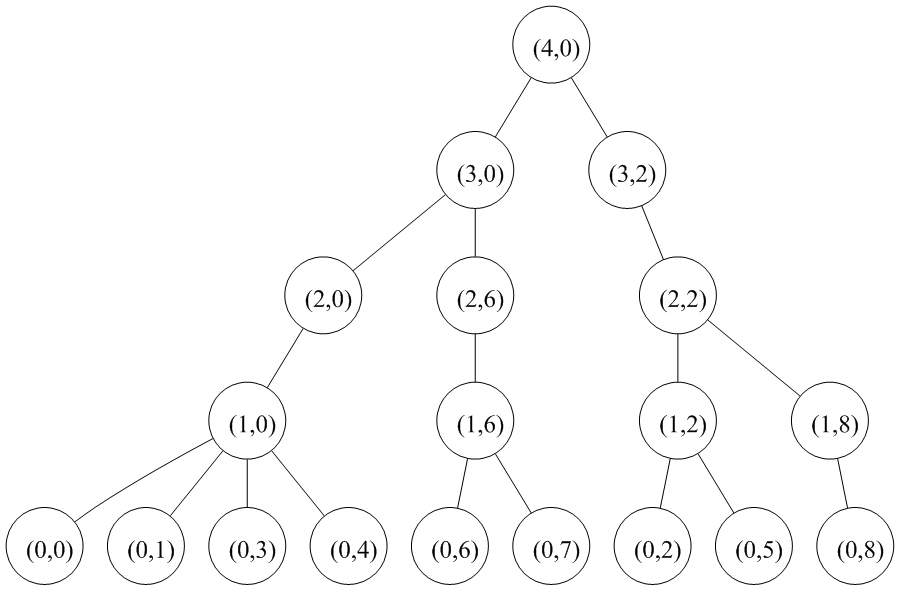
\includegraphics[width=8cm]{ipfs/ipfs-forest-layercloning-a-hierarchy.png}}%
	%
	\\
	%
	\subfigure[After cloning layer 2]
	{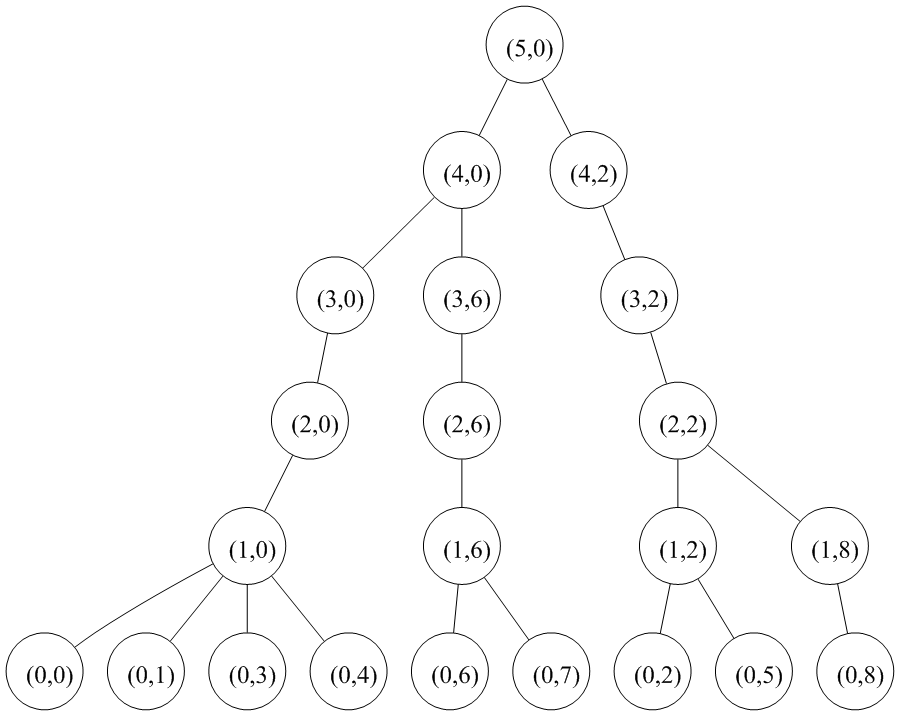
\includegraphics[width=8cm]{ipfs/ipfs-forest-layercloning-b-hierarchy.png}}%
\caption{An example of layer cloning.}
\label{fig:ipfs-forest-layercloning}
\end{stusubfig}
%---

\paragraph{C++ Method Interface}

\begin{lstlisting}[style=Prototype]
void clone_layer(int indexB);
\end{lstlisting}

\paragraph{User Interface for Image Analysis}

The simplest user interface just allows the user to clone the current layer by (for example) clicking on a menu item (see Figure~\ref{fig:ipfs-forest-layercloning-gui}). After cloning the layer, the interface can display the clone so that the user can begin working with it immediately. An alternative would be to allow the user to clone any layer in the forest by displaying a dialog box allowing them to choose the layer to be cloned, but in my view the former approach is more intuitive.

%---
\stufigex{height=5cm}{ipfs/ipfs-forest-layercloning-gui.png}{The user interface for layer cloning: a simple menu item allowing the current layer to be cloned.}{fig:ipfs-forest-layercloning-gui}{p}
%---

\paragraph{Precondition Checking}

The only precondition that needs checking for layer cloning is that the clonee (the layer being cloned) exists. This can be trivially checked in $O(1)$ time. Note that if the clone layer command is invoked from the user interface, the layer will inevitably exist (and we can skip the check), since the layer currently being viewed exists by definition.

\paragraph{Executing the Command}

Pseudo-code to execute a clone layer command is shown in Listing~\ref{code:ipfs-forest-clonelayerimpl}. The essence of the approach taken is simple: clone the graph of the layer below, then update the forest links between the clone layer and the layers below and above it. In order to implement the algorithm efficiently, however, it is important to employ a sensible iterator-based interface to the nodes in each forest layer: this allows us to iterate over the nodes in a layer in linear time and avoid the costly node lookups that might otherwise be necessary. Thus, in the pseudo-code, we iterate simultaneously over the nodes in the clonee layer and the clone, first propagating each parent link from the clonee node up to the clone node, then linking the corresponding nodes in the clonee and the clone together.

%---
\begin{stulisting}[!t]
\caption{Forest : Layer Cloning : Execution}
\label{code:ipfs-forest-clonelayerimpl}
\lstinputlisting[style=Default]{ipfs/ipfs-forest-clonelayerimpl.lst}
\end{stulisting}
%---

To analyse the complexity of the algorithm (referring to the listing), we proceed as follows. Firstly, let $L$ be the number of existing layers prior to the clone operation, and let $n_\ell$ be the number of nodes and $e_\ell$ be the number of adjacency graph edges in layer $\ell$. Let the clone layer being inserted be layer $c$ and the layer below it (from which it was cloned) be layer $b$. Then evidently $n_c = n_b$ and $e_c = e_b$.

Line $8$ is $O(1)$, because it only involves an array lookup. The complexity of Line $9$ differs depending on whether $b$ is a branch layer or the leaf layer. If it is a branch layer, then cloning the nodes in the graph is $O(n_b)$ and cloning the edges is $O(e_b)$, since these just involve cloning a tree-based data structure such as a std::map, which can be done in linear time. If $b$ is the leaf layer, then cloning the nodes is slightly trickier, because we need to create a std::map (the branch layer's representation for nodes) from a std::vector (the leaf layer's representation). However, as no sorting is actually required, this can still in principle be done in $O(n_b)$ time using a divide and conquer approach (na\"ive implementations, however, are more likely to end up being $O(n_b \log n_b)$). Cloning the edges is harder, because sorting may be required, although for regular grids it is in principle possible to devise a suitable scheme to traverse the edges in sorted order. If sorting can be avoided in this way, then cloning the edges takes $O(e_b)$; if not, it takes $O(e_b \log e_b)$. The total cost of Line $9$ is thus $O(n_b + e_b)$ when cloning a branch layer, and at worst $O(n_b \log n_b + e_b \log e_b)$ when cloning the leaf layer. Provided that $b$'s adjacency graph is connected (as are all the adjacency graphs dealt with in this thesis), $n_b \in O(e_b)$, in which case this simplifies to $O(e_b)$ for the branch layer case, and $O(e_b \log e_b)$ for the leaf layer case. Line $10$ is amortised $O(1)$, but for an individual operation can be $O(L)$ -- however, $L$ is generally a very small number. Lines $14-17$ are $O(1)$. Lines $19-23$ are $O(n_c) = O(n_b)$, since each iteration of the loop does a constant amount of work. In total, then the algorithm as a whole is (amortised) $O(e_b)$ in the branch layer case, and (amortised) $O(e_b \log e_b)$ in the leaf layer case.

\paragraph{Undoing the Command}

A clone layer command can be undone by simply deleting the clone (see Listing~\ref{code:ipfs-forest-deletelayerimpl} for pseudo-code). The complexity of this is analysed in the next section.

\index{partition forests!mutating algorithms!layer cloning|)}

\afterpage{\clearpage}
\newpage

%~~~~~~~~~~~~~~~~~~~~~~~~~~~~~~~~~~~~~~~~~~~~~~~~
\subsubsection{Layer Deletion}
%~~~~~~~~~~~~~~~~~~~~~~~~~~~~~~~~~~~~~~~~~~~~~~~~

\index{partition forests!mutating algorithms!layer deletion|(}

\paragraph{Description}

Any layer except the lowest can be deleted from the hierarchy (for example, see Figure~\ref{fig:ipfs-forest-layerdeletion}). In terms of the partition forest definition, this has the effect of removing both the specified partitioning graph from $\textit{PG}$ and the forest links referencing the deleted layer from $\textit{FL}$, and adding new forest links where necessary between any layers on either side of the one being removed.

%---
\begin{stusubfig}{p}
	\subfigure[Before deleting layer 1]
	{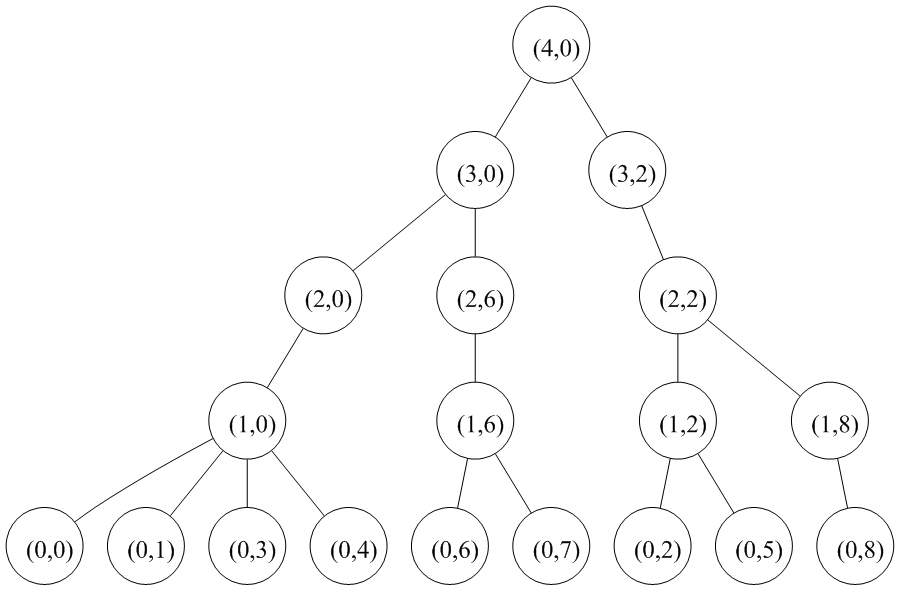
\includegraphics[width=10cm]{ipfs/ipfs-forest-layerdeletion-a-hierarchy.png}}%
	%
	\\
	%
	\subfigure[After deleting layer 1]
	{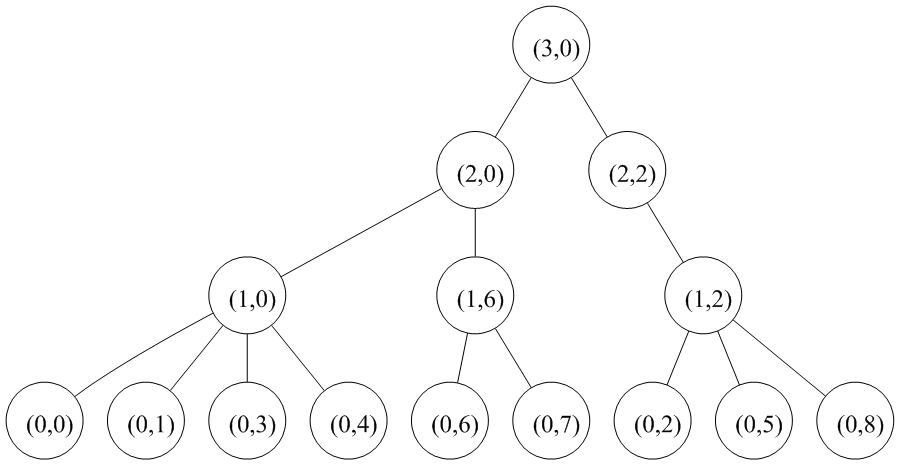
\includegraphics[width=10cm]{ipfs/ipfs-forest-layerdeletion-b-hierarchy.png}}%
\caption{An example of layer deletion.}
\label{fig:ipfs-forest-layerdeletion}
\end{stusubfig}
%---

\paragraph{C++ Method Interface}

\begin{lstlisting}[style=Prototype]
void delete_layer(int indexD);
\end{lstlisting}

\paragraph{User Interface for Image Analysis}

As with layer cloning, the simplest user interface just allows the user to delete the current layer by clicking on a menu item (see Figure~\ref{fig:ipfs-forest-layerdeletion-gui}).

%---
\stufigex{height=5cm}{ipfs/ipfs-forest-layerdeletion-gui.png}{The user interface for layer deletion: a simple menu item allowing the current layer to be deleted.}{fig:ipfs-forest-layerdeletion-gui}{p}
%---

\paragraph{Precondition Checking}

The only precondition that needs checking for layer deletion is that the layer being deleted is a branch layer. This is trivial to check in $O(1)$ time. (Depending on the design of the overall application, it may be necessary to make layer deletion slightly more constrained. For instance, an application that shows only branch layers may want to prevent the user from deleting the last branch layer, even though it's perfectly fine when viewed strictly from a partition forest perspective. Regardless, though, the required checks remain trivial.)

\paragraph{Executing the Command}

%---
\begin{stulisting}[p]
\caption{Forest : Layer Deletion : Execution}
\label{code:ipfs-forest-deletelayerimpl}
\lstinputlisting[style=Default]{ipfs/ipfs-forest-deletelayerimpl.lst}
\end{stulisting}
%---

%---
\begin{stulisting}[p]
\caption{Forest : Layer Deletion : Undo}
\label{code:ipfs-forest-undeletelayerimpl}
\lstinputlisting[style=Default]{ipfs/ipfs-forest-undeletelayerimpl.lst}
\end{stulisting}
%---

Pseudo-code to execute a delete layer command is shown in Listing~\ref{code:ipfs-forest-deletelayerimpl}. The idea is to update the forest links between the layers on either side of the layer to be deleted and then remove the layer itself from the forest. Specifically, if $D$ is the layer being deleted, $B$ is the layer below it and $A$ is the layer above (if it exists), then each node in $B$ should have its parent link updated to point to its grandparent in layer $A$. The grandparent nodes in $A$ should similarly have their child links updated to point to their grandchildren in layer $B$. To implement this efficiently, it is important to avoid calculating the grandchildren of nodes in $A$ explicitly. This is most easily arranged by iterating over the grandchildren and updating the grandparents during the course of the iteration (see pseudo-code). It is important to return the deleted layer (unchanged) at the end of the process, because it must be cached if we are to support undo.

We use the same notation to analyse the complexity as in the layer cloning analysis. Referring to the listing, line $16$ is a simple $O(1)$ array lookup. Lines $17-19$ are $O(n_a)$, since each iteration (if the loop happens at all) does a constant amount of work for each node in layer $A$. Lines $21-22$ are simple $O(1)$ array lookups. Lines $23-27$ are $O(n_b (\log n_d + \log n_a + \log \#\mathit{children}(\mathit{grandparentA}))) = O(n_b \log n_d)$, since $n_a \le n_d$ and $\#\mathit{children}(\mathit{grandparentA}) \le n_d$. Line $29$ is amortised $O(1)$. The algorithm as a whole is $O(n_a + n_b \log n_d) = O(n_b \log n_d)$, since $n_a \le n_b$.

\paragraph{Undoing the Command}

Pseudo-code to undo a delete layer command is shown in Listing~\ref{code:ipfs-forest-undeletelayerimpl}. The algorithm reinserts the deleted layer $D$ (cached during deletion) back into the forest, then recreates the forest links in the layers below ($B$) and above ($A$, where applicable) the deletion point, using the links in the deleted layer to discover which links to add.

(It is worth observing that undeleting a layer in an interactive system may not necessarily be as simple as this. One good reason for deleting a layer is to save memory, in particular the substantial amount of memory associated with the textures that display the partition forest to the user. Caching these textures when deleting a layer would in this case defeat the point of deleting the layer in the first place. A compromise solution is to cache the layer itself, but delete the textures -- we then arrange to recreate the textures from scratch in the event that the layer is undeleted.)

In terms of complexity, line $8$ in the listing is amortised $O(1)$. Lines $12-15$ are $O(n_a)$, because they involve a simple array lookup, followed by at most a constant time operation for each node in layer $A$. Line $17$ is a simple $O(1)$ array lookup. Lines $18-21$ are more interesting: note that line $20$, which involves an $O(\log n_b)$ lookup, executes exactly $n_b$ times (we're running through the children of every node in the layer above $B$, i.e.~through all the nodes actually in $B$), so the cost of the first part of the loop is $O(n_b \log n_b)$. Line $21$, by contrast, executes $n_d$ times and involves at most $O(\log n_a + \log \#\mathit{children}(\mathit{n.parent()}))$ amount of work each time, adding $O(n_d (\log n_a + \log \#\mathit{children}(\mathit{n.parent()})))$ work to the total. This is dominated by the earlier $O(n_b \log n_b)$, which is thus the total cost of lines $18-21$. The cost of the entire algorithm, bearing in mind that line $8$'s cost was amortised, and that $n_a \le n_b$, is thus amortised $O(n_b \log n_b)$.

\index{partition forests!mutating algorithms!layer deletion|)}

\afterpage{\clearpage}
\newpage

%~~~~~~~~~~~~~~~~~~~~~~~~~~~~~~~~~~~~~~~~~~~~~~~~
\subsubsection{Sibling Node Merging}
%~~~~~~~~~~~~~~~~~~~~~~~~~~~~~~~~~~~~~~~~~~~~~~~~

\index{partition forests!mutating algorithms!sibling node merging|(}

\paragraph{Description}

Sibling nodes in any layer of the hierarchy other than the lowest can be merged provided that the union of the objects they represent is contiguous (this condition ensures that the new node post-merging still represents a valid object). A set of nodes are siblings if they either all have the same parent, or all have no parent (the latter case occurs when the nodes are in the top layer of the hierarchy, when they are all implicitly children of the top-level object represented by the partition forest -- e.g.~the whole image in the case of an image partition forest). The algorithm takes as input the set of sibling nodes to be merged, and returns the node resulting from the merge. An example is shown in Figure~\ref{fig:ipfs-forest-siblingnodemerging}.

%---
\begin{stusubfig}{p}
	\subfigure[The forest before the merge.]
	{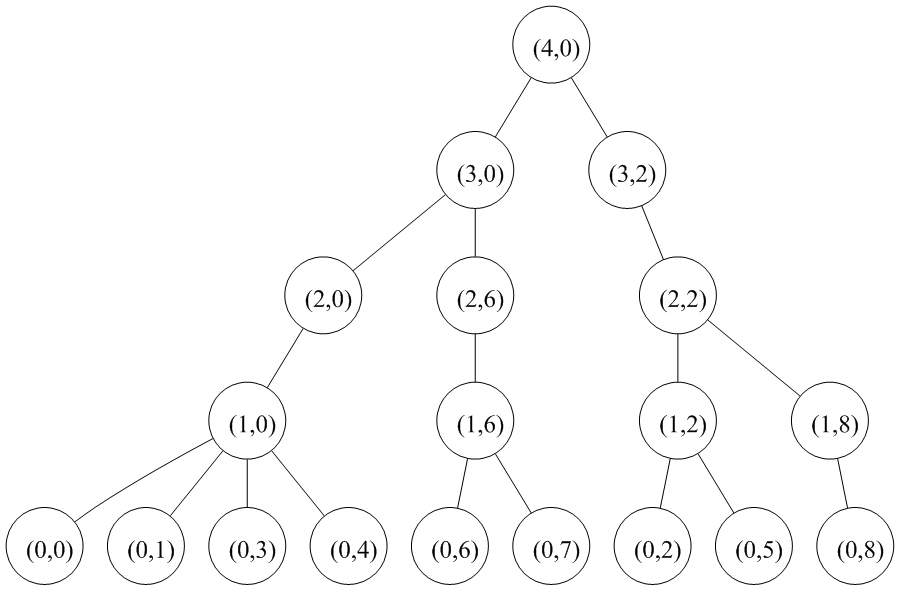
\includegraphics[width=.7\linewidth]{ipfs/ipfs-forest-siblingnodemerging-a-hierarchy.png}}%
	%
	\hspace{8mm}%
	%
	\subfigure[The layer 2 graph before the merge.]
	{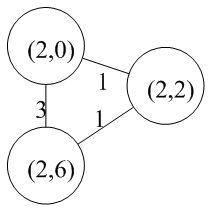
\includegraphics[width=.2\linewidth]{ipfs/ipfs-forest-siblingnodemerging-a-graph2.png}}%
	%
	\hspace{8mm}%
	%
	\subfigure[The forest after the merge.]
	{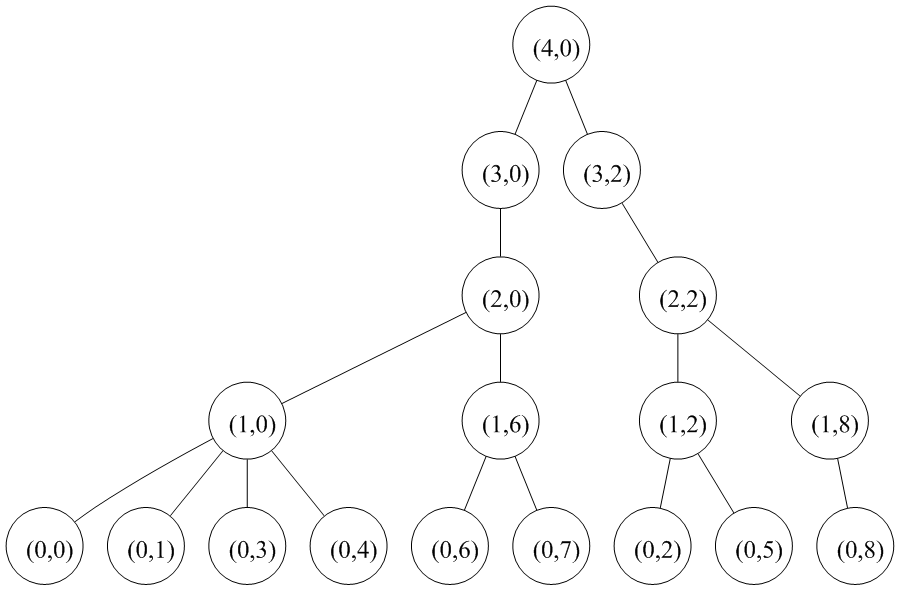
\includegraphics[width=.7\linewidth]{ipfs/ipfs-forest-siblingnodemerging-b-hierarchy.png}}%
	%
	\hspace{8mm}%
	%
	\subfigure[The layer 2 graph after the merge.]
	{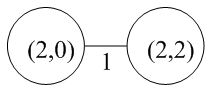
\includegraphics[width=.2\linewidth]{ipfs/ipfs-forest-siblingnodemerging-b-graph2.png}}%
\caption{An example of sibling node merging: merging nodes (2,0) and (2,6).}
\label{fig:ipfs-forest-siblingnodemerging}
\end{stusubfig}
%---

\paragraph{C++ Method Interface}

\begin{lstlisting}[style=Prototype]
NodeID merge_sibling_nodes(const set<NodeID>& nodes);
\end{lstlisting}

\paragraph{User Interface for Image Analysis}

Although it is a crucial operation, it doesn't make sense to expose sibling-only node merging in the interface, since that would require the user to keep track of which nodes share the same forest parent. A much better solution (shown later) is to expose the more intuitive operation that merges arbitrary nodes in the same layer into their connected components.

\paragraph{Precondition Checking}

The following preconditions must be checked for sibling node merging (see the pseudo-code in Listing~\ref{code:ipfs-forest-mergesiblingnodes} for the method):

\begin{enumerate}

\item There must be more than one node to be merged. (This can be trivially checked in $O(1)$ time.)
\item None of the nodes must be in the lowest layer of the forest. (This can be checked in time $O(\#\mathit{nodes})$.)
\item The nodes must share a common parent in the forest. Note that this implies that they must all be in the same layer. (Assuming the nodes share a common layer $m$, then the cost of looking up the parent for each node is $O(\log n_m)$, whence the total cost of this check is $O(\#\mathit{nodes} \log n_m)$.)
\item The union of the objects represented by the nodes to be merged must be connected. (This can be checked in $O(\#\mathit{nodes} \log e_m)$ time. To see this, examine the \texttt{are_connected} and \texttt{find_connected_component} listings in Appendix~\ref{chap:appendixpf}. The worst case is when all the nodes must be visited, i.e.~when there is a single connected component. When that happens, over the course of the process, every node is erased from the set of input nodes and inserted into the set of result nodes -- $O(\#\mathit{nodes} \log \#\mathit{nodes})$ overall. Each node is also pushed onto the queue and popped off it again -- $O(\#\mathit{nodes})$ overall. Every node but the seed is also looked up during the \texttt{contains} call -- $O(\#\mathit{nodes} \log \#\mathit{nodes})$ overall. The dominant cost of $O(\#\mathit{nodes} \log e_m)$ comes from having to look up the adjacent edges for each input node in the tree-based data structure storing the edges for forest layer $m$.)

\end{enumerate}

\noindent The overall cost of checking the preconditions is thus $O(\#\mathit{nodes} \log e_m)$, since $n_m \in O(e_m)$ (the adjacency graphs we're dealing with are connected).

%---
\begin{stulisting}[p]
\caption{Forest : Sibling Node Merging : Precondition Checking}
\label{code:ipfs-forest-mergesiblingnodes}
\lstinputlisting[style=Default]{ipfs/ipfs-forest-mergesiblingnodes.lst}
\end{stulisting}
%---

%---
\begin{stulisting}[p]
\caption{Forest : Sibling Node Merging : Command}
\label{code:ipfs-forest-mergesiblingnodescommand}
\lstinputlisting[style=Default]{ipfs/ipfs-forest-mergesiblingnodescommand.lst}
\end{stulisting}
%---

\paragraph{Executing the Command}

%---
\begin{stulisting}[p]
\caption{Forest : Sibling Node Merging : Execution}
\label{code:ipfs-forest-mergesiblingnodesimpl}
\lstinputlisting[style=Default]{ipfs/ipfs-forest-mergesiblingnodesimpl.lst}
\end{stulisting}
%---

Pseudo-code to execute a sibling node merge command is shown in Listing~\ref{code:ipfs-forest-mergesiblingnodesimpl}. Firstly, the mergee node with the lowest index is picked to be the result of the merge (for instance, nodes $(2,2)$, $(2,1)$ and $(2,5)$ in a hypothetical forest would be merged into a new node called $(2,1)$, since $\min(\{2,1,5\}) = 1$). This node is referred to as the `canonical' node in the code.

In Step 1, forest links are then added (in both directions) between the canonical node and the children of the other nodes being merged (the parent links from the children to the canonical node replace those already there; the child links in the other direction are simply added). If the nodes being merged are not in the highest layer, the forest links joining the non-canonical nodes to their common parent must also be removed (since the non-canonical nodes will ultimately be removed from the forest).

As a result of merging the other nodes into the canonical node, the latter may gain new edges that it did not have before (since some of the other nodes may have been adjacent to nodes that it itself was not), and its properties (such as its voxel count) will generally change. In Step 2, therefore, its edges are updated using the edges of the other nodes. When there is a duplicate edge (i.e.~both the canonical node and one of the other nodes have an edge to a third node), then a new edge weight has to be chosen -- depending on the scheme in use, this might for example involve taking the minimum of the weights on the two existing edges (the appropriate method for a lowest pass point approach). Also in Step 2, the canonical node's properties are recalculated directly from those of its children (note that this is why the partition forest definition places direct calculability constraints on property sets).

Finally, Step 3 removes the non-canonical nodes. In the pseudo-code given (based on my implementation in \emph{millipede}), this also has the effect of removing any edges adjacent to those nodes -- if an alternative implementation strategy is chosen, however, these may need to be removed manually.

In terms of complexity analysis, we first let $k$ be the number of nodes to be merged. Line $6$ in Listing~\ref{code:ipfs-forest-mergesiblingnodesimpl} is $O(1)$, since the nodes in the input set are sorted by index. Line $7$ is $O(k)$, since it involves a set copy followed by an erase. Lines $8-9$ are $O(1)$, since they are array lookups. Line $16$ is $O(\log n_m)$ due to the set lookup done by \texttt{node_children}. Lines $17-20$ require more careful analysis. There is $O(k \log n_m)$ work looking up the children of the $k-1$ nodes in \texttt{others}. The inner loop runs $\sum_{x \in \mathit{others}} \#children(x)$ times, and does an $O(\log n_b)$ set lookup and a set insertion into \texttt{canonicalChildren} that is guaranteed to be no worse than $O(\log n_b)$ on each iteration. Thus, lines $17-20$ are $O(k \log n_m + (\sum_{x \in \mathit{others}} \#\mathit{children}(x)) \log n_b)$ overall. Lines $24-29$ do $O(\log n_m + \log n_a + k \log \#\mathit{parentChildren})$ work, made up of a layer $M$ node lookup, a layer $A$ node lookup and $k-1$ set erases from \texttt{parentChildren}. Lines $34-38$ again require careful analysis. The layer $M$ adjacent edge lookups in the outer loop require $O(k \log e_m)$ work. The inner loop runs $\sum_{x \in \mathit{others}} \#\mathit{adjacent\_edges}(x)$ times, and does $O(\log e_m)$ work updating the edge weight on each iteration. Thus, lines $34-38$ involve $O(k \log e_m + (\sum_{x \in \mathit{others}} \#\mathit{adjacent\_edges}(x)) \log e_m)$ work overall. Line $41$ is $O(\sum_{x \in \mathit{nodes}} \#\mathit{children}(x))$. Line $42$ is an $O(\log n_m)$ layer $M$ node lookup. Lines $46-47$ are $O(k(\log n_m + \log e_m))$, since they involve removing each of the $k-1$ nodes being merged from the layer $M$ node set and their adjacent edge sets from the layer $M$ edge table (a single erase is required in each case). This simplifies to $O(k \log e_m)$, since $n_m \in O(e_m)$.

Although I will not show the long-winded derivation here, the complexity of the algorithm as a whole can be simplified down to:
%
\begin{eqnarray*}
O(\#children(\mathit{canonical}) \; + \\
\left(\sum_{x \in others} \#\mathit{children}(x)\right) \log n_b \; + \\
\left(\sum_{x \in \mathit{others}} \#\mathit{adjacent\_edges}(x)\right) \log e_m)
\end{eqnarray*}
%
Simplifying even further, this can be upper-bounded by $O(n_b \log n_b + e_m \log e_m)$, or even just $O(e_b \log e_b)$, since both $n_b$ and $e_m$ are $\le e_b$.

\paragraph{Undoing the Command}

To undo a sibling node merge command, the intuition is that the node resulting from the merge must be split back into the nodes that were originally merged to create it. As we will see in the next section, however, a node is split not by specifying the \emph{nodes} into which to split it (these do not exist prior to the split, so that approach doesn't work), but by specifying connected groups of the node's children: a parent is generated for each of these groups and the node to be split is replaced with the group parents. For that reason, if we want to be able to undo a sibling node merge then we must store the children of each of the nodes to be merged when we initially execute the command. The merge can then be undone by splitting the merge result back into the components specified by the stored child groups (see Listing~\ref{code:ipfs-forest-mergesiblingnodescommand} for the detailed implementation).

\index{partition forests!mutating algorithms!sibling node merging|)}

\afterpage{\clearpage}
\newpage

%~~~~~~~~~~~~~~~~~~~~~~~~~~~~~~~~~~~~~~~~~~~~~~~~
\subsubsection{Node Splitting}
%~~~~~~~~~~~~~~~~~~~~~~~~~~~~~~~~~~~~~~~~~~~~~~~~

\index{partition forests!mutating algorithms!node splitting|(}

\paragraph{Description}

Nodes in any layer of the hierarchy other than the lowest can be split into multiple nodes representing smaller objects. (Note that the definition of objects requires that each of these smaller objects must be contiguous.) The algorithm takes as input the node to be split, and a set of groups of the node's children into which to split it, where each group is a set of child nodes. It returns the nodes created by the split. An example is shown in Figure~\ref{fig:ipfs-forest-nodesplitting}.

%---
\begin{stusubfig}{p}
	\subfigure[The forest before the split.]
	{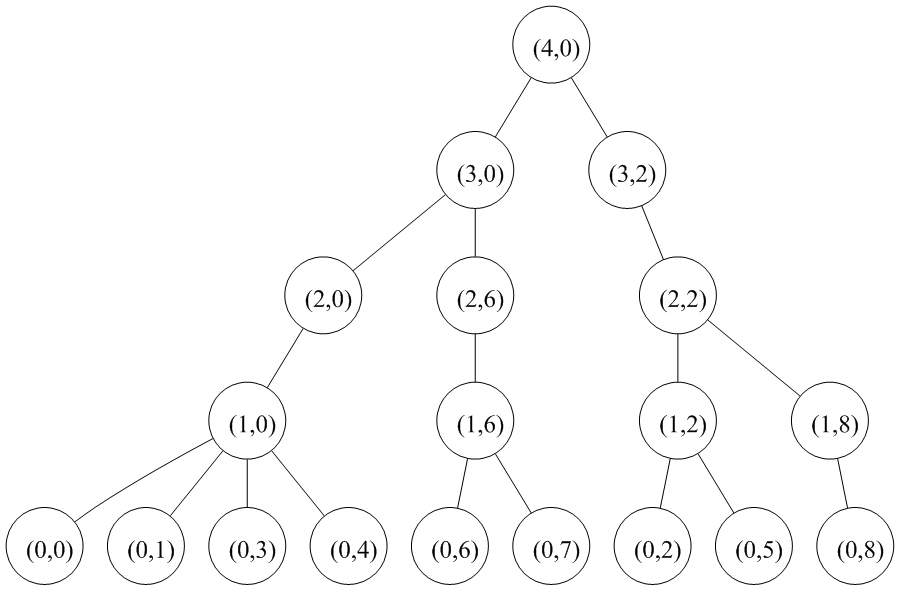
\includegraphics[width=.65\linewidth]{ipfs/ipfs-forest-nodesplitting-a-hierarchy.png}}%
	%
	\hspace{8mm}%
	%
	\subfigure[The layer 1 graph before the split.]
	{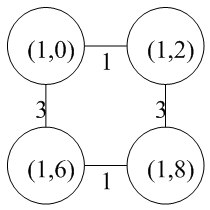
\includegraphics[width=.25\linewidth]{ipfs/ipfs-forest-nodesplitting-a-graph1.png}}%
	%
	\hspace{8mm}%
	%
	\subfigure[The forest after the split.]
	{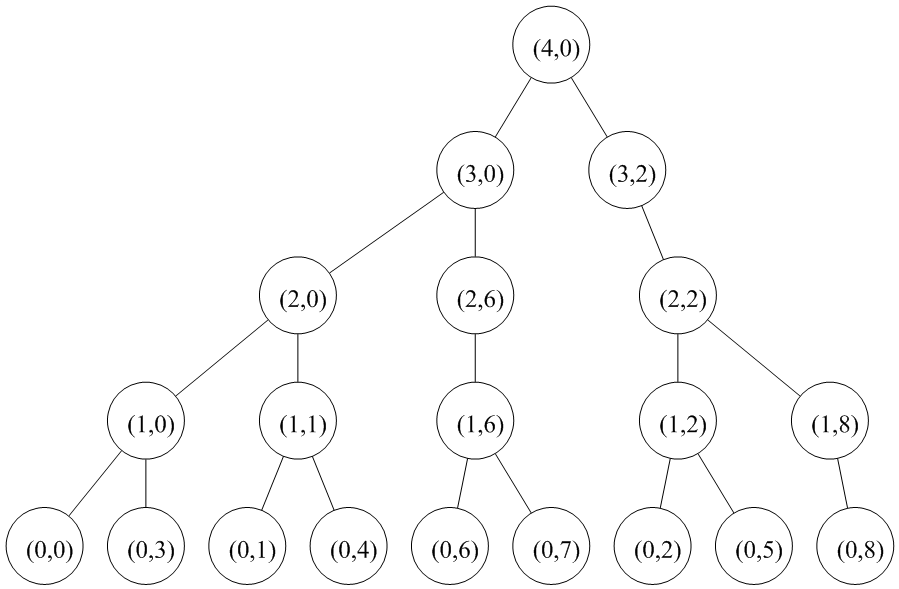
\includegraphics[width=.65\linewidth]{ipfs/ipfs-forest-nodesplitting-b-hierarchy.png}}%
	%
	\hspace{8mm}%
	%
	\subfigure[The layer 1 graph after the split.]
	{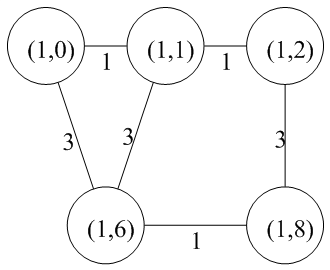
\includegraphics[width=.25\linewidth]{ipfs/ipfs-forest-nodesplitting-b-graph1.png}}%
\caption{An example of node splitting: splitting node (1,0) into two.}
\label{fig:ipfs-forest-nodesplitting}
\end{stusubfig}
%---

\paragraph{C++ Method Interface}

\begin{lstlisting}[style=Prototype]
set<NodeID> split_node(const NodeID& node,
                       const vector<set<int> >& groups);
\end{lstlisting}

\paragraph{User Interface for Image Analysis}

The user interface for node splitting is necessarily more complicated than that for earlier operations, because the user needs to be able to indicate the way in which a node should be split. As illustrated in Figure~\ref{fig:ipfs-forest-nodesplitting-gui}, this is a multi-step operation. The user initially selects and marks a node to be split, then defines the components into which it should be split by iteratively selecting and marking connected subgroups of its children. (If a mistake is made, it is possible to remove a subgroup and try again, although this is not illustrated for space reasons.) As the illustrated example implies, any remaining unmarked children will be automatically divided into subgroups by finding their connected components (this substantially reduces the work that has to be done by the user). Finally, the user `finalizes' the split and the desired changes are made to the forest.

%---
\begin{stusubfig}{p}
	\subfigure[Select the node to be split in the forest]
	{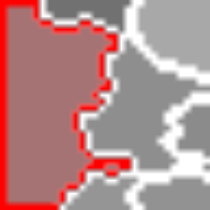
\includegraphics[width=.2\linewidth]{ipfs/ipfs-forest-nodesplitting-gui-a.png}}%
	%
	\hspace{8mm}%
	%
	\subfigure[Mark it to be split by clicking the menu item]
	{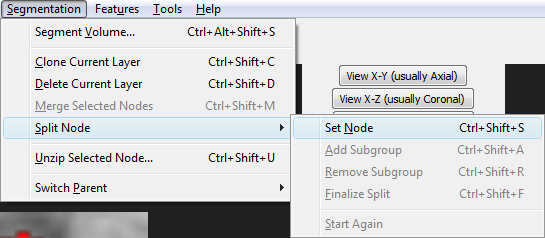
\includegraphics[width=.5\linewidth]{ipfs/ipfs-forest-nodesplitting-gui-b.png}}%
	%
	\hspace{8mm}%
	%
	\subfigure[After marking it, its children will be highlighted]
	{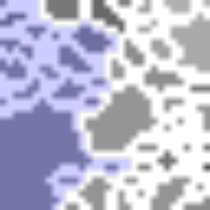
\includegraphics[width=.2\linewidth]{ipfs/ipfs-forest-nodesplitting-gui-c.png}}%
	%
	\hspace{8mm}%
	%
	\subfigure[Select the child nodes in a subgroup]
	{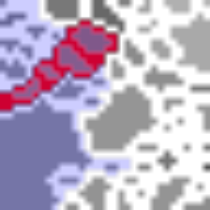
\includegraphics[width=.2\linewidth]{ipfs/ipfs-forest-nodesplitting-gui-d.png}}%
	%
	\hspace{8mm}%
	%
	\subfigure[Add the subgroup by clicking the menu item]
	{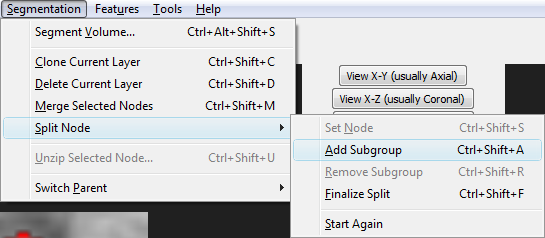
\includegraphics[width=.5\linewidth]{ipfs/ipfs-forest-nodesplitting-gui-e.png}}%
	%
	\hspace{8mm}%
	%
	\subfigure[Each subgroup will be assigned a different colour]
	{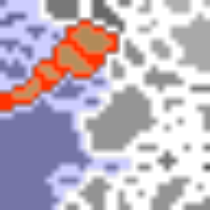
\includegraphics[width=.2\linewidth]{ipfs/ipfs-forest-nodesplitting-gui-f.png}}%
	%
	\hspace{8mm}%
	%
	\subfigure[Repeat (d)-(f) to add other subgroups, then finalize the split by clicking the menu item]
	{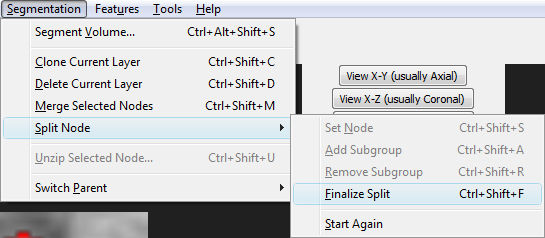
\includegraphics[width=.5\linewidth]{ipfs/ipfs-forest-nodesplitting-gui-g.png}}%
	%
	\hspace{8mm}%
	%
	\subfigure[The node will be split as indicated]
	{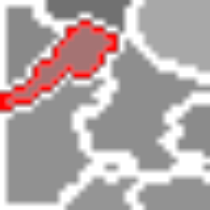
\includegraphics[width=.2\linewidth]{ipfs/ipfs-forest-nodesplitting-gui-h.png}}%
\caption{The user interface for node splitting}
\label{fig:ipfs-forest-nodesplitting-gui}
\end{stusubfig}
%---

\paragraph{Precondition Checking}

%---
\begin{stulisting}[t]
\caption{Forest : Node Splitting : Precondition Checking}
\label{code:ipfs-forest-splitnode}
\lstinputlisting[style=Default]{ipfs/ipfs-forest-splitnode.lst}
\end{stulisting}
%---

The following preconditions must be checked for node splitting (see the pseudo-code in Listing~\ref{code:ipfs-forest-splitnode} for the method):

\begin{enumerate}

\item The node to be split must not be in the leaf layer of the forest. (This can be trivially checked in $O(1)$ time.)
\item The node to be split must exist. (This can be checked in $O(1)$ time for the leaf layer, and $O(\log n_s)$ time for branch layer $s$.)
\item There must be more than one subgroup. (This can be trivially checked in $O(1)$ time.)
\item The subgroups must partition the children of the node being split. (This can be checked in time $O(C \log C)$, where $C$ is the number of children.)
\item Each of the subgroups must be non-empty and connected. (Each of the $G$ groups requires $O(1)$ time for the non-empty check, and $O(\#\mathit{group} \log e_b)$ time to check connectedness, where $b$ is the layer containing the group nodes.)

\end{enumerate}

When implementing node splitting in a user interface like the one described above, these preconditions should be checked by the interface, not by the forest at the time of finalizing the split. The user should not, for example, have the option of adding invalid subgroups or finalizing a split without defining any subgroups.

\paragraph{Executing the Command}

Pseudo-code to execute a split node command is shown in Listing~\ref{code:ipfs-forest-splitnodeimpl}. In Step 1, the node to be split is deleted from the forest -- this involves removing the forest links that connect the node to its parent and children, and removing the node itself from the partitioning graph for its forest layer (in the pseudo-code, removing the node from the graph also removes its adjacent edges). In Step 2, each of the groups of children that define a node resulting from the split is used to generate a new node in the split layer (a parent for the group). This new node has the index of the lowest-indexed child node (for instance, the parent of nodes $(1,5)$, $(1,3)$ and $(1,7)$ in a hypothetical forest would be denoted $(2,3)$). Its properties are calculated by combining those of its children in the usual way. Forest links are added to connect the new node to its children in the group and its parent in the layer above (namely the parent of the node that is being split). Finally, in Step 3, the adjacency graph for the split layer is locally reconstructed around the nodes resulting from the split (it was locally destroyed when the node being split was removed) -- this is done by considering all the edges adjacent to any of the split node's children, and propagating them upwards to the split layer. For instance, if node $p_1$ in the split layer has children $c_1$ and $c_2$, and node $p_2$ in the split layer has children $c_3$ and $c_4$, and the only edges between children of $p_1$ and $p_2$ are $(\{c_1,c_3\}, w_{13})$ and $(\{c_2,c_4\}, w_{24})$, then this induces an edge $(\{p_1,p_2\}, f(w_{13}, w_{24}))$ in the split layer, where $f$ is some appropriate function on edge weights, such as $\min$ in the case of a lowest pass point approach.

%---
\begin{stulisting}[t]
\caption{Forest : Node Splitting : Execution}
\label{code:ipfs-forest-splitnodeimpl}
\lstinputlisting[style=Default]{ipfs/ipfs-forest-splitnodeimpl.lst}
\end{stulisting}
%---

In terms of complexity analysis, lines $4-6$ in Listing~\ref{code:ipfs-forest-splitnodeimpl} are $O(1)$. Lines $11-12$ are $O(\log n_s + \#\mathit{children}(node) \log n_b)$. Line $14$ is $O(\log n_s)$. Line $15$ is $O(\log n_a + \log \#\mathit{children}(\mathit{parentIndex})) = O(\log n_a)$. Line $18$ is $O(\log n_s + \log e_s)$, since removing the node also involves a lookup in the edge table to remove the node's set of adjacent edges. This simplifies to $O(\log e_s)$. Lines $22-31$ require more careful analysis -- we analyse each line over all $\#\mathit{groups}$ iterations of the loop. Line $24$ requires $O(1)$ for each iteration and thus $O(\#\mathit{groups})$ overall. Line $25$ involves inserting $\#\mathit{groups}$ nodes into a set, and is thus $O(\#\mathit{groups} \log \#\mathit{groups})$ overall. Line $26$ requires $O(\#\mathit{groups} \log n_s)$ for the lookups done by \texttt{set_node_properties}, and $O(\sum_{\mathit{group} \in \mathit{groups}} \#\mathit{group})$ for combining the properties of the various groups. Lines $27$ and $28$ each require $O(\#\mathit{groups} \log n_s)$ for the lookups they do. Lines $29-30$ involve a layer $B$ lookup for each node in every group, and are thus $O((\sum_{\mathit{group} \in \mathit{groups}} \#\mathit{group}) \log n_b)$. Line $31$ requires $O(\#\mathit{groups} \log n_a)$ work for the child lookups, and $O(\#\mathit{groups} \log \#\mathit{groups})$ for the set insertions. The overall complexity of lines $22-31$ is thus $O((\sum_{\mathit{group} \in \mathit{groups}} \#\mathit{group}) \log n_b)$. Lines $34-40$ also require careful analysis. Each iteration of the innermost loop does an $O(\log e_b)$ lookup of adjacent edges, and then $O(\#\mathit{adjacent\_edges}(n) (\log n_b + \log e_s))$ work actually updating edge weights. The overall complexity of lines $34-40$ is:
%
\[
O\left( \sum_{\mathit{group} \in \mathit{groups}} \sum_{n \in \mathit{group}} (\log e_b + \#\mathit{adjacent\_edges}(n) (\log n_b + \log e_s)) \right)
\]
%
This is also the complexity of the entire algorithm, since the edge propagation step is the dominant cost involved. To simplify this further, at the cost of a looser upper bound, observe that $n$ iterates over all the children of the node being split, so this becomes:
%
\[
O\left( \sum_{n \in \mathit{children}(node)} (\log e_b + \#\mathit{adjacent\_edges}(n) (\log n_b + \log e_s)) \right)
\]
%
Since $\#\mathit{children}(node) \le n_b$, the first part of the sum is $O(n_b \log e_b)$. The second part is $O(e_b (\log n_b + \log e_s))$, since each edge in the layer below can only appear as the adjacent edge of at most two children. A simpler upper-bound for the entire algorithm is thus just $O(e_b (\log n_b + \log e_s))$, or even just $O(e_b \log e_b)$, since both $n_b$ and $e_s$ are $\le e_b$.

\paragraph{Undoing the Command}

To undo a split node command, it is enough to just re-merge the results of the split using a sibling node merge (see Listing~\ref{code:ipfs-forest-mergesiblingnodesimpl} for pseudo-code).

\index{partition forests!mutating algorithms!node splitting|)}

\afterpage{\clearpage}
\newpage

%################################################
\subsection{Zipping Algorithms}
%################################################

Whilst the core mutating algorithms provide all that is theoretically required for partition forest editing, certain operations are nevertheless tedious for the user to perform using only these primitives. For instance, it seems intuitively sensible that the user should be able to merge not only nodes that are siblings in the forest, but any nodes that are adjacent in the graph for their forest layer. Such `higher-level' algorithms, however, require more substantial changes to the structure of the forest; in particular, they require changes to be made in more than one layer.

In order to facilitate the implementation of such algorithms, it is helpful to introduce two intermediary forest operations that I call \emph{unzip node} (or just \emph{unzipping}) and \emph{zip chains} (or just \emph{zipping}). These are respectively multi-layer split and merge operations on the forest, and can be implemented in terms of their lower-level counterparts. In fact, such an approach is not only possible but advisable, since it can be used to avoid writing special code to undo the operations. The key is to introduce an entity called a \emph{listener-alerting command sequence guard}. This is created at the start of a composite operation like an unzip, and informs both the application's command manager and any listeners that a command sequence is about to start (in C++, this would happen in the constructor for the guard). The relevant lower-level commands are then executed, after which the guard is destroyed again, informing the application's command manager and any listeners that the command sequence has ended (in C++, this would happen in the guard's destructor). Undoing the composite operation is then a simple matter of undoing the lower-level commands in reverse order, something that can be easily handled by any decent command manager implementation. Bearing this in mind, we can now examine each of the zipping algorithms in detail.

\newpage

%~~~~~~~~~~~~~~~~~~~~~~~~~~~~~~~~~~~~~~~~~~~~~~~~
\subsubsection{Unzipping}
%~~~~~~~~~~~~~~~~~~~~~~~~~~~~~~~~~~~~~~~~~~~~~~~~

\index{partition forests!mutating algorithms!unzipping|(}

\paragraph{Description}

A node in any layer of the hierarchy can be unzipped to a specified higher layer (or the top of the hierarchy). This essentially `separates out' the branch from the higher layer down to the specified node: it is effectively a multi-layer split, with a set containing the node in question as one of the groups at each stage. The key issue that has to be addressed in order to make this work is the need to find the other groups for each split: the algorithm presented here solves this problem by defining the other groups to be the connected components of what is left after removing the node being unzipped from consideration. See Figure~\ref{fig:ipfs-forest-unzipping} for an example.

%---
\begin{stusubfig}{p}
	\subfigure[Initial hierarchy]{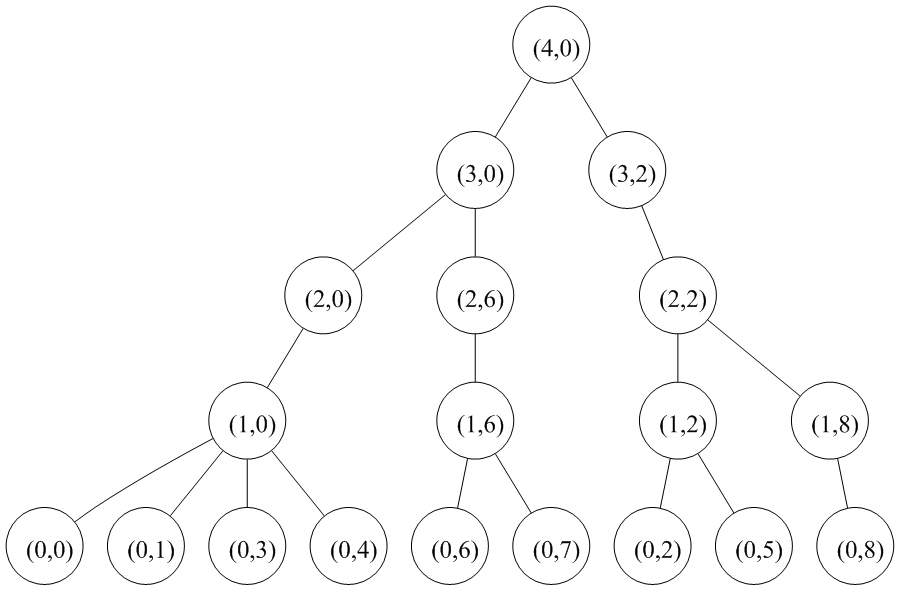
\includegraphics[width=.45\linewidth]{ipfs/ipfs-forest-unzipping-a-hierarchy.png}}%
	\hspace{8mm}%
	\subfigure[After splitting $(1,2)$]{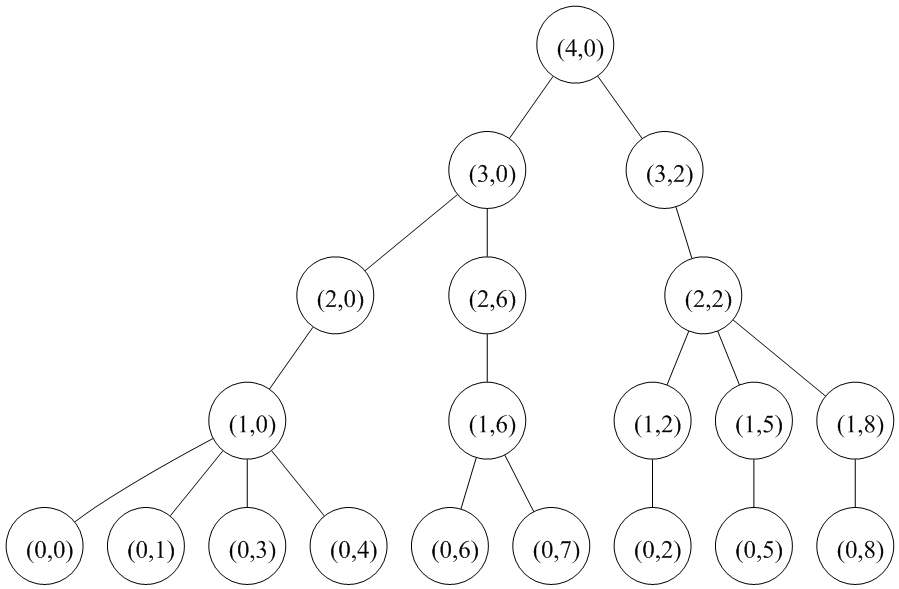
\includegraphics[width=.45\linewidth]{ipfs/ipfs-forest-unzipping-b-hierarchy.png}}%
	\\
	\subfigure[After splitting $(2,2)$]{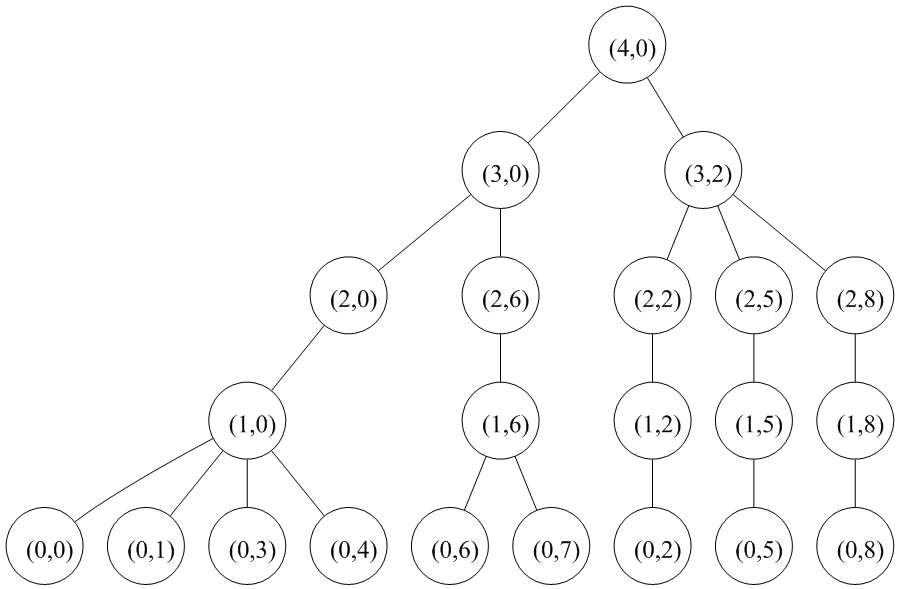
\includegraphics[width=.45\linewidth]{ipfs/ipfs-forest-unzipping-c-hierarchy.png}}%
	\hspace{8mm}%
	\subfigure[After splitting $(3,2)$]{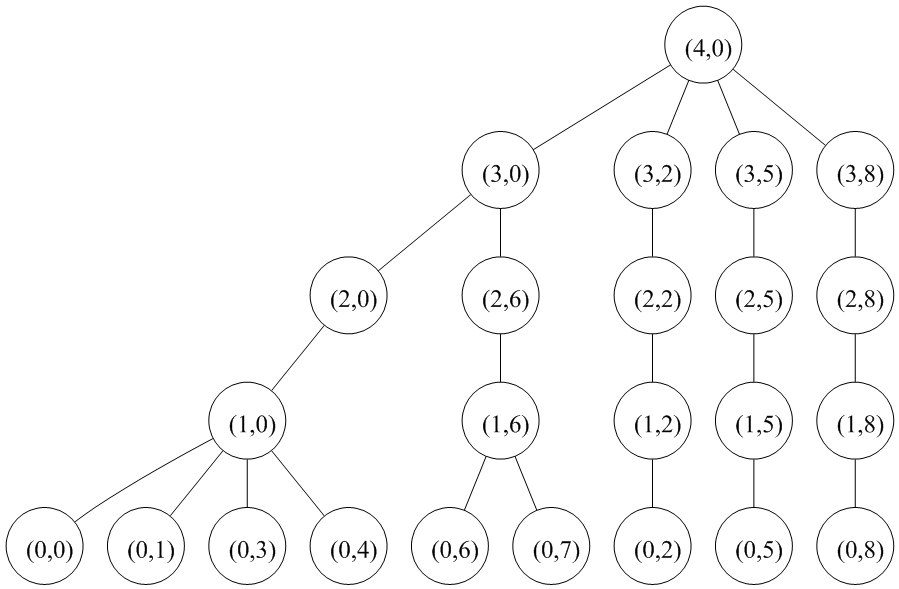
\includegraphics[width=.45\linewidth]{ipfs/ipfs-forest-unzipping-d-hierarchy.png}}%
	\\
	\subfigure[Initial layer $1$ graph]{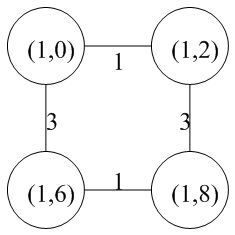
\includegraphics[width=.22\linewidth]{ipfs/ipfs-forest-unzipping-a-graph1.png}}%
	\hspace{8mm}%
	\subfigure[Initial layer $2$ graph]{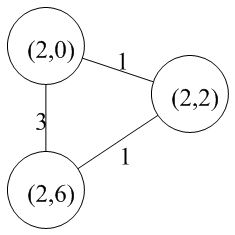
\includegraphics[width=.22\linewidth]{ipfs/ipfs-forest-unzipping-a-graph2.png}}%
	\hspace{8mm}%
	\subfigure[Initial layer $3$ graph]{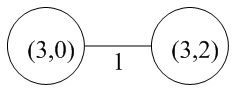
\includegraphics[width=.22\linewidth]{ipfs/ipfs-forest-unzipping-a-graph3.png}}%
	\\
	\subfigure[Final layer $1$ graph]{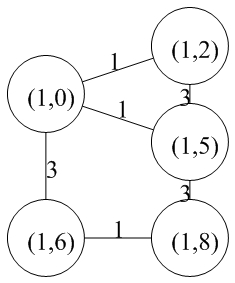
\includegraphics[width=.22\linewidth]{ipfs/ipfs-forest-unzipping-b-graph1.png}}%
	\hspace{8mm}%
	\subfigure[Final layer $2$ graph]{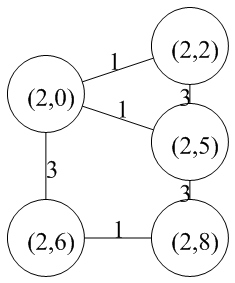
\includegraphics[width=.22\linewidth]{ipfs/ipfs-forest-unzipping-c-graph2.png}}%
	\hspace{8mm}%
	\subfigure[Final layer $3$ graph]{\includegraphics[width=.22\linewidth]{ipfs/ipfs-forest-unzipping-d-graph3.png}}%
\caption{An example of unzipping: unzipping node $(0,5)$ to layer $3$}
\label{fig:ipfs-forest-unzipping}
\end{stusubfig}
%---

The algorithm takes as input the node to be unzipped and the (higher) layer to which to unzip it. It returns a set of chains that could in theory be passed to the zipping algorithm described below in order to undo the operation, although undo is actually handled automatically when unzipping is implemented as a composite operation. A \emph{chain} is a sequence of nodes $[n_h,\ldots,n_\ell]$, where $h \ge \ell$, $n_i$ is in layer $i$ and $\forall i \in [\ell,h) \cdot \mbox{parent}(n_i) = n_{i+1}$. It should be noted that the chains returned by the unzipping algorithm are not necessarily all of the same length, but they all start in the same layer of the hierarchy.

\paragraph{C++ Method Interface}

\begin{lstlisting}[style=Prototype]
typedef deque<NodeID> Chain;
vector<Chain> unzip_node(const NodeID& node, int toLayer);
\end{lstlisting}

\paragraph{User Interface for Image Analysis}

The user interface for unzipping is relatively straightforward, as illustrated in Figure~\ref{fig:ipfs-forest-unzipping-gui}. The user selects a node, then clicks a menu item to indicate that it should be unzipped. This brings up a dialog box that allows the user to choose the target layer of the unzip. After the user enters the target layer, the node is then unzipped as desired.

%---
\begin{stusubfig}{p}
	\subfigure[Layer 1 before unzipping]
	{\hspace{2mm}\includegraphics[width=.25\linewidth]{ipfs/ipfs-forest-unzipping-gui-a.png}\hspace{2mm}}%
	\hspace{8mm}%
	\subfigure[Layer 2 before unzipping]
	{\hspace{2mm}\includegraphics[width=.25\linewidth]{ipfs/ipfs-forest-unzipping-gui-b.png}\hspace{2mm}}%
	\\
	\subfigure[Layer 3 before unzipping]
	{\hspace{2mm}\includegraphics[width=.25\linewidth]{ipfs/ipfs-forest-unzipping-gui-c.png}\hspace{2mm}}%
	\hspace{8mm}%
	\subfigure[Select a node to unzip]
	{\hspace{2mm}\includegraphics[width=.25\linewidth]{ipfs/ipfs-forest-unzipping-gui-d.png}\hspace{2mm}}%
	\\
	\subfigure[Click the menu item]{\includegraphics[width=.4\linewidth]{ipfs/ipfs-forest-unzipping-gui-e.png}}%
	\hspace{8mm}%
	\subfigure[Enter the target layer]{\includegraphics[width=.4\linewidth]{ipfs/ipfs-forest-unzipping-gui-f.png}}%
	\\
	\subfigure[Layer 2 after unzipping]
	{\hspace{2mm}\includegraphics[width=.25\linewidth]{ipfs/ipfs-forest-unzipping-gui-g.png}\hspace{2mm}}%
	\hspace{8mm}%
	\subfigure[Layer 3 after unzipping]
	{\hspace{2mm}\includegraphics[width=.25\linewidth]{ipfs/ipfs-forest-unzipping-gui-h.png}\hspace{2mm}}%
\caption{The user interface for unzipping}
\label{fig:ipfs-forest-unzipping-gui}
\end{stusubfig}
%---

\paragraph{Precondition Checking}

The following preconditions must be checked for unzipping:

\begin{enumerate}

\item The node being unzipped must exist. (This can be checked in $O(1)$ time for the leaf layer, and $O(\log n_\ell)$ time for branch layer $\ell$.)
\item If $L$ is the layer containing the node being unzipped, and $H$ is the highest layer in the partition forest, then the index of the layer to which to unzip must be in the range $[L,H]$. (This can be trivially checked in $O(1)$ time.)

\end{enumerate}

\paragraph{Implementation}

Pseudo-code implementing the unzipping algorithm is shown in Listing~\ref{code:ipfs-forest-unzipnode}. As the algorithm progresses, we keep track of node chains that represent the strands being unzipped: these will be what is eventually returned as the result. In each iteration of the loop, we keep track of a `current' node, initially the input node. We determine the siblings of this node (defined to be the other children of its parent) and calculate their connected components. To these we add a singleton component containing the current node itself. We then split the parent of the current node into the specified components, update the aforementioned chains and repeat the process with the parent of the current node. The loop terminates when we reach the user-specified target layer.

The construction of the chains is the most interesting part of the algorithm. The way this works is most easily demonstrated by stepping through the unzipping example illustrated in Figure~\ref{fig:ipfs-forest-unzipping}. Initially, the array of chains is initialised with a singleton chain containing only the node being unzipped: in this case $(0,5)$.\footnote{This is an implementation trick that ensures that the chain leading up from the node being unzipped is the first chain in the array: this allows it to be easily identified by other algorithms that need ready access to it, such as \texttt{merge_nonsibling_nodes} (they would otherwise have to search through all the chains to find it). The final chain should not contain the actual node being unzipped (only the nodes above it), so in practice we remove it from the end of the chain again before returning.} During each iteration of the loop, each node resulting from that iteration's split node operation will either be used to augment an existing chain, or to add a new one: specifically, each existing chain is prepended with the parent of its head node, which is then removed from the set of nodes resulting from the split (it is guaranteed to be present because of the way the algorithm works); the remaining nodes resulting from the split are then used to create new singleton chains. In this example, the first iteration of the loop (in which \texttt{cur} = $(0,5)$, \texttt{parent} = $(1,2)$, \texttt{components} = $[\{2\}, \{5\}]$ and \texttt{result} = $\{(1,2), (1,5)\}$) results in \texttt{chains} being set to $[[(1,5), (0,5)], [(1,2)]]$. The second iteration (in which \texttt{cur} = $(1,5)$, \texttt{parent} = $(2,2)$, \texttt{components} = $[\{2\}, \{5\}, \{8\}]$ and \texttt{result} = $\{(2,2), (2,5), (2,8)\}$) results in \texttt{chains} being set to $[[(2,5), (1,5), (0,5)], [(2,2), (1,2)], [(2,8)]]$. The third iteration (in which \texttt{cur} = $(2,5)$, \texttt{parent} = $(3,2)$, \texttt{components} = $[\{2\}, \{5\}, \{8\}]$ and \texttt{result} = $\{(3,2), (3,5), (3,8)\}$) results in \texttt{chains} being set to $[[(3,5), (2,5), (1,5), (0,5)], [(3,2), (2,2), (1,2)], [(3,8), (2,8)]]$. Finally, $(0,5)$ is removed from the first chain, leaving the final chains to be returned by the algorithm as $[[(3,5), (2,5), (1,5)], [(3,2), (2,2), (1,2)], [(3,8), (2,8)]]$.

%---
\begin{stulisting}[p]
\caption{Forest : Unzipping : Implementation}
\label{code:ipfs-forest-unzipnode}
\lstinputlisting[style=Default]{ipfs/ipfs-forest-unzipnode.lst}
\end{stulisting}
%---

\paragraph{Complexity Analysis}

The complexity of executing an unzip operation (ignoring the precondition checking) is most easily characterised in terms of the complexity of the underlying node splitting operations. In Listing~\ref{code:ipfs-forest-unzipnode}, lines $15-22$ and $55$ are all clearly $O(1)$, so we focus instead on the main loop in lines $24-50$. Consider the iteration of this loop in which $cur.layer() = c$, and let $p = c+1$. Then line $26$ is $O(\log n_c)$, since it involves a layer $c$ node lookup. Line $27$ is a simple $O(1)$ array lookup. Line $28$ is $O(\log n_p)$ for the child lookup, $O(\#\mathit{children}(parent))$ for the set copy and $O(\log \#\mathit{children}(parent))$ for the set erase. Line $31$ is $O(\#\mathit{siblings} \log e_c)$, since \texttt{find_connected_components} has the same complexity as \texttt{are_connected}, which was analysed previously. Line $34$ is $O(1)$. Line $35$ is $O(\mathit{split\_node\_cost}(parent, ccs))$. Lines $38-42$ require careful analysis. In each iteration, line $39$ requires $O(1)$ work. Line $40$ requires $O(\log n_c)$ work, since $h$ is guaranteed to be in layer $c$ by the way the algorithm works. Line $41$ is clearly $O(1)$, since \texttt{chain} is a deque. To analyse line $42$, we have to consider all $\#\mathit{chains}$ iterations of the loop -- at worst, we erase every element of the result set by the end of the loop. Its initial size was the number of connected components into which we split the node, or $\#\mathit{ccs}$, so the worst case complexity of all the erases in line $42$ is $O(\log(\#\mathit{ccs}!))$. Overall, lines $38-42$ have complexity $O(\#\mathit{chains} \log n_c + \log(\#\mathit{ccs}!))$. Continuing with the rest of the outer loop, Lines $44-47$ clearly have worst case complexity $O(\#\mathit{ccs})$, since they do a constant amount of work for all the remaining nodes in \texttt{result}, and result's initial size was $\#\mathit{ccs}$. Finally, line $50$ is $O(\log n_c)$ for the layer $c$ node lookup.

Analysing the algorithm as a whole, it is clear from the above that the only significant costs involved are in lines $31$, $35$ and $38-42$, i.e.~in determining how to split the node, splitting it, and updating the chains. Of these, the most costly is evidently splitting the node. Bearing in mind the outer loop involved, and letting $u = \mathit{node.layer()}$, the overall complexity of the algorithm thus becomes:
%
\[
O\left( \sum_{i=u}^{\mathit{toLayer} - 1} \mathit{split\_node\_cost}(\mathit{parent}_i, \mathit{ccs}_i) \right)
\]
%
The observation to be made from this is that the complexity of the unzip is the same as the sum of the complexities of the individual splits it entails -- the work involved to find the splits and to update the chains is far less costly and can be ignored. To simplify this further, recall that the cost of splitting a node in layer $s$ is $O(e_{s-1} \log e_{s-1})$. The complexity here thus becomes:
%
\[
O\left( \sum_{i=u}^{\mathit{toLayer} - 1} (e_{i-1} \log e_{i-1}) \right)
\]
%
In the worst case, $e_{\mathit{toLayer}-2} = \ldots = e_{u-1}$, and this simplifies to:
%
\[
O((toLayer-u) e_{u-1} \log e_{u-1})
\]

\index{partition forests!mutating algorithms!unzipping|)}

\afterpage{\clearpage}
\newpage

%~~~~~~~~~~~~~~~~~~~~~~~~~~~~~~~~~~~~~~~~~~~~~~~~
\subsubsection{Zipping}
%~~~~~~~~~~~~~~~~~~~~~~~~~~~~~~~~~~~~~~~~~~~~~~~~

\index{partition forests!mutating algorithms!zipping|(}

\paragraph{Description}

A set of node chains (see the description of unzipping for a definition) that all start in the same layer can be zipped together, an operation that is effectively a multi-layer sibling node merge. When performed on the results of an unzip, this effectively undoes that operation. The zipping algorithm takes as input $k$ chains $[n_{1h},\ldots,n_{1\ell_1}], \ldots, [n_{kh},\ldots,n_{k\ell_k}]$ and returns a pair consisting of a node and a layer index, namely the parameters that we would need to pass to \texttt{unzip_node} in order to undo the operation. See Figure~\ref{fig:ipfs-forest-zipping} for an example.

%---
\begin{stusubfig}{p}
	\subfigure[Initial hierarchy]{\includegraphics[width=.43\linewidth]{ipfs/ipfs-forest-zipping-a-hierarchy.png}}%
	\hspace{8mm}%
	\subfigure[After merging layer $3$ nodes]{\includegraphics[width=.43\linewidth]{ipfs/ipfs-forest-zipping-b-hierarchy.png}}%
	\\
	\subfigure[After merging layer $2$ nodes]{\includegraphics[width=.43\linewidth]{ipfs/ipfs-forest-zipping-c-hierarchy.png}}%
	\hspace{8mm}%
	\subfigure[After merging layer $1$ nodes]{\includegraphics[width=.43\linewidth]{ipfs/ipfs-forest-zipping-d-hierarchy.png}}%
	\\
	\subfigure[Initial layer $1$ graph]{\includegraphics[width=.22\linewidth]{ipfs/ipfs-forest-zipping-a-graph1.png}}%
	\hspace{8mm}%
	\subfigure[Initial layer $2$ graph]{\includegraphics[width=.22\linewidth]{ipfs/ipfs-forest-zipping-a-graph2.png}}%
	\hspace{8mm}%
	\subfigure[Initial layer $3$ graph]{\includegraphics[width=.22\linewidth]{ipfs/ipfs-forest-zipping-a-graph3.png}}%
	\\
	\subfigure[Final layer $1$ graph]{\includegraphics[width=.22\linewidth]{ipfs/ipfs-forest-zipping-d-graph1.png}}%
	\hspace{8mm}%
	\subfigure[Final layer $2$ graph]{\includegraphics[width=.22\linewidth]{ipfs/ipfs-forest-zipping-c-graph2.png}}%
	\hspace{8mm}%
	\subfigure[Final layer $3$ graph]{\includegraphics[width=.22\linewidth]{ipfs/ipfs-forest-zipping-b-graph3.png}}%
\caption{An example of zipping: zipping together the four chains $[(3,0), (2,6), (1,6)]$, $[(3,2), (2,2)]$, $[(3,5), (2,5)]$ and $[(3,8), (2,8), (1,8)]$}
\label{fig:ipfs-forest-zipping}
\end{stusubfig}
%---

\paragraph{C++ Method Interface}

\begin{lstlisting}[style=Prototype]
typedef deque<NodeID> Chain;
pair<NodeID,int> zip_chains(const vector<Chain>& chains);
\end{lstlisting}

\paragraph{User Interface for Image Analysis}

It doesn't make sense to expose zipping as part of the user interface, since the inputs it requires (node chains) are too cumbersome for the user to be asked to provide directly. More usable operations such as parent switching (described in the next section), that use zipping internally, should be exposed instead.

\paragraph{Precondition Checking}

The preconditions to be checked for zipping can be deduced from the preconditions required by the sibling node merges in terms of which it is implemented. There are at least two reasons for enforcing the preconditions at the zip level, rather than letting them be checked internally by the merges:

\begin{enumerate}

\item Zipping should be an \emph{atomic} forest operation -- that is, if the zip fails, the forest should be unchanged. Checking at the merge level can result in the zip being aborted after changes have been made to the forest, potentially leaving it in an inconsistent state.

\item Checking at the zip level is slightly more efficient -- in particular, we can exploit our knowledge about the sequence of merges to be performed in order to avoid checking in all but the top-most layer that the nodes to be merged are siblings.

\end{enumerate}

\noindent The following checks are thus necessary (see Listing~\ref{code:ipfs-forest-zipchains} for pseudo-code):

\begin{enumerate}

\item There must be chains to zip.% (This can be trivially checked in $O(1)$ time.)
\item Each chain must be non-empty and consist only of valid nodes.
\item No chain must extend down as far as the leaf layer of the forest -- this guarantees that we will not be trying to merge leaf layer nodes.% (This can be checked in $O(\#\mathit{chains})$ time.)
\item The highest nodes in the chains must be siblings of each other. Note that there is no need to check that other corresponding nodes in the chains are siblings, as merging their parents in the previous iteration of the loop will automatically guarantee that they share the same parent.
\item The sets of nodes to be merged in each layer must be connected.

\end{enumerate}

\paragraph{Implementation}

Pseudo-code for the zipping algorithm is shown in Listing~\ref{code:ipfs-forest-zipchains}. The actual implementation is entirely straightforward (all the real work is in checking the preconditions). We start by determining the high and low layers of the chains. All the chains share the same high layer, so it suffices to take the high layer of the first chain in the array. The low layer is determined by a simple minimum element operation on the low layers of each of the individual chains. For each of the layers, from the top down, the relevant nodes are then extracted from the chains and merged using sibling node merging (note that there is no need to re-check the preconditions for each merge).

%---
\begin{stulisting}[p]
\caption{Forest : Zipping : Implementation}
\label{code:ipfs-forest-zipchains}
\lstinputlisting[style=Default]{ipfs/ipfs-forest-zipchains.lst}
\end{stulisting}
%---

\paragraph{Complexity Analysis}

The complexity of executing a zip operation (ignoring the precondition checking) is most easily characterised in terms of the complexity of the underlying sibling node merging operations. In Listing~\ref{code:ipfs-forest-zipchains}, line $33$ is clearly $O(1)$ and lines $34-36$ are clearly $O(\#\mathit{chains})$. Lines $40-46$ can be analysed as follows. Each iteration of the outer loop first constructs a set of at most $\#\mathit{chains}$ nodes by inserting them one at a time -- this involves $O(\log(\#\mathit{chains}!))$ work, as usual. It then merges the nodes in this set, with the cost as given in the sibling node merging analysis. Since the dominant cost in this is in merging the nodes, not in constructing the sets of nodes to be merged, the overall complexity of the loop, and ultimately the algorithm as a whole, is then
%
\[
O\left( \sum_{m=\mathit{lowLayer}}^{\mathit{highLayer}} \mathit{sibling\_node\_merge\_cost}(\mathit{nodes}_m) \right),
\]
%
where $\mathit{nodes}_m$ is the set of nodes to be merged in layer $m$. In other words, the complexity of a zip is the sum of the complexities of the sibling node merges it has to do -- all the other work involved is far less costly than the actual merges. To simplify this further, recall that the cost of merging sibling nodes in layer $m$ is $O(e_{m-1} \log e_{m-1})$. The complexity here thus becomes:
%
\[
O\left( \sum_{m=\mathit{lowLayer}}^{\mathit{highLayer}} e_{m-1} \log e_{m-1} \right)
\]
%
In the worst case, $e_{\mathit{highLayer}-1} = \ldots = e_{\mathit{lowLayer}-1}$, and this simplifies to:
%
\[
O((highLayer+1-lowLayer) e_{\mathit{lowLayer}-1} \log e_{\mathit{lowLayer}-1})
\]

\index{partition forests!mutating algorithms!zipping|)}

\afterpage{\clearpage}
\newpage

%################################################
\subsection{Higher-Level Algorithms}
%################################################

Having discussed unzipping and zipping in the previous section, we are now in a position to implement two higher-level partition forest algorithms that are of great practical use. The first of these is the previously-mentioned merging operation that allows the user to merge nodes based on their adjacency in their forest layer (i.e.~in an imaging context, their spatial adjacency within the image) rather than whether or not they share a common forest parent. As observed earlier, this is the `intuitive' merging operation that the user wants to perform on forest nodes, but it is a difficult operation to implement without the machinery provided by the zipping algorithms.

The second higher-level algorithm that we can now implement is parent switching, the problem tackled in a more constrained manner by Peter Nacken in \cite{nacken95}. This operation mutates the forest so as to move a node from being the child of one parent to the child of another parent. As discussed in \S\ref{sec:background-partitionhierarchies}, there are two cases when this is problematic: (1) when the node is not adjacent to its new parent and (2) when moving the node would divide its old parent. Nacken's approach prevents nodes being moved in either of these two cases. There is clearly nothing that can be done about case (1) -- if the node is not adjacent to its new parent, then it can never be combined with the new parent's children to form a valid node. However, we will see that it is possible to use the zipping algorithms described here to develop a less constrained version of parent switching that still works in case (2) situations. (It should nevertheless be noted that Nacken's original analysis is entirely correct: it is not possible to switch the parent of a node in case (2) whilst keeping the old parent intact. The approach which I will describe circumvents this problem by allowing the old parent to be fragmented by the switch operation.)

\newpage

%~~~~~~~~~~~~~~~~~~~~~~~~~~~~~~~~~~~~~~~~~~~~~~~~
\subsubsection{Non-Sibling Node Merging}
%~~~~~~~~~~~~~~~~~~~~~~~~~~~~~~~~~~~~~~~~~~~~~~~~

\index{partition forests!mutating algorithms!non-sibling node merging|(}

\paragraph{Description}

A set of arbitrary nodes in any layer of the hierarchy other than the lowest can be divided into its connected components, each of which can then be merged. Since each component is connected, the result of each merge represents a valid object. From the user's perspective, this is a far more intuitive merge operation than sibling node merging: they simply have to indicate a set of nodes in a particular layer, and these are then merged into as few connected components as possible, based on their adjacency in the layer's graph. There is no requirement that the selected nodes are connected, or that they share a common parent (thus the user is freed from having to think about the structure of the forest when performing a merge). The algorithm takes as input the set of nodes to be merged, and returns the set of nodes resulting from merging each of the input's connected components (i.e.~there is one output node for each connected component of the input). An example is shown in Figure~\ref{fig:ipfs-forest-nonsiblingnodemerging}.

%---
\begin{stusubfig}{p}
	\subfigure[Initial hierarchy]{\includegraphics[width=.45\linewidth]{ipfs/ipfs-forest-nonsiblingnodemerging-a-hierarchy.png}}%
	\hspace{8mm}%
	\subfigure[After unzipping $(1,0)$ and $(1,2)$ to layer $2$]{\includegraphics[width=.45\linewidth]{ipfs/ipfs-forest-nonsiblingnodemerging-c-hierarchy.png}}%
	\\
	\subfigure[{After zipping $[(2,0), (1,0)]$ and $[(2,2), (1,2)]$}]{\includegraphics[width=.45\linewidth]{ipfs/ipfs-forest-nonsiblingnodemerging-d-hierarchy.png}}%
	\hspace{8mm}%
	\subfigure[After unzipping $(1,6)$ and $(1,8)$ to layer $2$]{\includegraphics[width=.45\linewidth]{ipfs/ipfs-forest-nonsiblingnodemerging-f-hierarchy.png}}%
	\\
	\subfigure[{After zipping $[(2,6), (1,6)]$ and $[(2,8), (1,8)]$}]{\includegraphics[width=.45\linewidth]{ipfs/ipfs-forest-nonsiblingnodemerging-g-hierarchy.png}}%
\caption{An example of non-sibling node merging: merging nodes $(1,0)$, $(1,2)$, $(1,6)$ and $(1,8)$}
\label{fig:ipfs-forest-nonsiblingnodemerging}
\end{stusubfig}
%---

\paragraph{C++ Method Interface}

\begin{lstlisting}[style=Prototype]
set<NodeID> merge_nonsibling_nodes(const set<NodeID>& nodes);
\end{lstlisting}

\paragraph{User Interface for Image Analysis}

The user interface for non-sibling node merging is very simple, as illustrated in Figure~\ref{fig:ipfs-forest-nonsiblingnodemerging-gui}. The user selects some nodes, then clicks a menu item to merge them.

%---
\begin{stusubfig}{p}
	\hspace{.1\linewidth}%
	\subfigure[Layer 2 before merging]
	{\includegraphics[width=.3\linewidth]{ipfs/ipfs-forest-nonsiblingnodemerging-gui-a.png}}%
	%
	\hspace{8mm}%
	%
	\subfigure[Select the nodes to be merged]
	{\hspace{.05\linewidth}\includegraphics[width=.3\linewidth]{ipfs/ipfs-forest-nonsiblingnodemerging-gui-b.png}\hspace{.05\linewidth}}%
	%
	\\
	%
	\subfigure[Click the menu item]
	{\includegraphics[width=.4\linewidth]{ipfs/ipfs-forest-nonsiblingnodemerging-gui-c.png}}%
	%
	\hspace{8mm}%
	%
	\subfigure[Layer 2 after merging]
	{\includegraphics[width=.3\linewidth]{ipfs/ipfs-forest-nonsiblingnodemerging-gui-d.png}}%
\caption{The user interface for non-sibling node merging.}
\label{fig:ipfs-forest-nonsiblingnodemerging-gui}
\end{stusubfig}
%---

\paragraph{Precondition Checking}

The great advantage of non-sibling node merging over sibling node merging is that it has fewer preconditions; in fact, it owes its existence to the need to provide a less-constrained, more user-friendly merging algorithm for partition forest. It is therefore unsurprising that its preconditions are a strict subset of those of sibling node merging:

\begin{enumerate}

\item There must be more than one node to be merged. (This can be trivially checked in $O(1)$ time.)
\item None of the nodes must be in the lowest layer of the forest. (This can be checked in time linear in the number of nodes.)

\end{enumerate}

\paragraph{Implementation}

Pseudo-code to implement non-sibling node merging is shown in Listing~\ref{code:ipfs-forest-mergenonsiblingnodes}. The first step is to calculate the connected components of the input nodes: each connected component of size $> 1$ will be merged into one result node. To actually perform the merging for each connected component, we determine the common ancestor of the component's nodes. Each node is then unzipped to the layer below that containing the ancestor. In each case we keep track of the chain of nodes leading back down to the node being unzipped, appending the actual node being unzipped to the chain in each case (it would not otherwise be present). Finally, all of these chains are zipped together to merge the nodes in the connected component together.

For the example given in Figure~\ref{fig:ipfs-forest-nonsiblingnodemerging}, the connected components of the input nodes are $\{(1,0), (1,2)\}$ and $\{(1,6), (1,8)\}$. Both $(1,0)$ and $(1,2)$ are unzipped to layer $2$, the layer below their common ancestor $(3,0)$. The strands thus created are then zipped together, resulting in $(1,0)$ and $(1,2)$ being merged in layer $1$. An analogous process is used to merge $(1,6)$ and $(1,8)$.

%---
\begin{stulisting}[p]
\caption{Forest : Non-Sibling Node Merging : Implementation}
\label{code:ipfs-forest-mergenonsiblingnodes}
\lstinputlisting[style=Default]{ipfs/ipfs-forest-mergenonsiblingnodes.lst}
\end{stulisting}
%---

\paragraph{Complexity Analysis}

In terms of complexity analysis, we must first analyse the complexity of \texttt{find_common_ancestor_layer} (see Listing~\ref{code:appendixpf-findcommonancestorlayer}). In that listing, line $4$ is clearly $O(1)$. Within the loop in lines $5$--$11$, lines $6$, $7$, $10$ and $11$ are only $O(1)$ per iteration, and can therefore be discounted. The interesting part of the code is lines $8$--$9$. Observe that $\#\mathit{curs}$ is initially equal to $\#\mathit{component}$, and then drops to $1$ in a non-increasing manner. As an upper-bound, we may therefore safely assume that the worst case is when $\#\mathit{curs}$ stays at $\#\mathit{component}$ until the highest layer is reached, at which point it drops to $1$, i.e.~that there are always $O(\#\mathit{component})$ iterations of the inner loop. Letting $\ell = \mathit{layerIndex}$, the cost per iteration of the parent lookup in line $9$ is clearly $O(\log n_\ell)$, whence the cost of parent lookups over all iterations is $O(\#\mathit{component} \log n_\ell)$. Over all iterations of the loop, the cost of the set insertions in line $9$ is $O(\log(\#\mathit{component}!))$. The total cost of the inner loop is thus $O(\#\mathit{component} \log n_\ell + \log(\#\mathit{component}!))$. Letting $\ell_0$ be the initial value of $\mathit{layerIndex}$, and $L = \mathit{highest\_layer()}$, the overall complexity of the function as a whole is thus:
%
\[
O\left( \sum_{\ell=\ell_0}^L (\#\mathit{component} \log n_\ell + \log(\#\mathit{component}!)) \right)
\]
%
Since $\log(\#\mathit{component}!)$ is $O(\#\mathit{component} \log \#\mathit{component})$, and both $n_\ell$ and $\#\mathit{component}$ are $\le n_{\ell_0}$, this simplifies to:
%
\[
O\left( \sum_{\ell=\ell_0}^L \#\mathit{component} \log n_{\ell_0} \right)
\]
%
Since nothing inside the sum depends on $\ell$, this becomes $O((L+1-\ell_0) \#\mathit{component} \log n_{\ell_0})$, or even just $O(L n_{\ell_0} \log n_{\ell_0})$.

Returning to \texttt{merge_nonsibling_nodes} in Listing~\ref{code:ipfs-forest-mergenonsiblingnodes}, lines $19$--$23$ are trivially $O(1)$. Lines $24$--$25$ are $O(\log(\#\mathit{nodes}!))$. As per previous analysis of \texttt{find_connected_components}, line $26$ is $O(\#\mathit{indices} \log e_m) = O(\#\mathit{nodes} \log e_m)$, where $m$ is the layer containing the nodes being merged. The major cost of the function clearly comes from the loop in lines $29$--$51$. Per iteration, line $30$ is clearly $O(1)$. By the analysis above, line $34$ is $O((L+1-m) \#\mathit{component} \log n_m)$. Line $41$ is $O(1)$. The inner loop in lines $42$--$47$ requires more analysis. Within that loop, everything except the unzip in line $45$ is clearly $O(1)$ or amortised $O(1)$, which we can discount. The unzip itself is run for every node in $\mathit{nodes}$. In the worst case, each node may be unzipped to the top of the hierarchy. Bearing in mind the earlier analysis of unzip, the overall work (over all iterations of the outer loop) done by line $45$ is thus $O(\#\mathit{nodes} (L+1-m) e_{m-1} \log e_{m-1})$. The final line in the outer loop, line $51$, does two things: a zip operation and an insertion into the \texttt{mergedNodes} set. Over all iterations of the outer loop, the insertions only cost $O(\log(\#\mathit{ccs}!))$, so they can be discounted. As per earlier analysis of zip, each zip here is $O((L+1-m) e_{m-1} \log e_{m-1})$, making the total complexity for zip over all iterations of the loop $O(\#\mathit{ccs} (L+1-m) e_{m-1} \log e_{m-1})$. The complexity of the algorithm as a whole is thus dominated by the cost of the unzips (since $\#\mathit{ccs} \le \#\mathit{nodes}$), and is simply:
%
\[
O(\#\mathit{nodes} (L+1-m) e_{m-1} \log e_{m-1})
\]

\index{partition forests!mutating algorithms!non-sibling node merging|)}

\afterpage{\clearpage}
\newpage

%~~~~~~~~~~~~~~~~~~~~~~~~~~~~~~~~~~~~~~~~~~~~~~~~
\subsubsection{Parent Switching}
%~~~~~~~~~~~~~~~~~~~~~~~~~~~~~~~~~~~~~~~~~~~~~~~~

\index{partition forests!mutating algorithms!parent switching|(}

\paragraph{Description}

A node in any layer of the hierarchy except the highest can be moved from being the child of its parent node to being the child of another node in the layer above, provided that it is adjacent to at least one child of its new parent. It is possible that moving the node may cause some of its old ancestors to become disconnected. If this happens, what remains of each old ancestor is split into its connected components. The algorithm takes as input the node to be moved and the index of its new parent node in the layer above. See Figure~\ref{fig:ipfs-forest-parentswitch} for an example.

%---
\begin{stusubfig}{p}
	\subfigure[The initial hierarchy]{\includegraphics[width=.5\linewidth]{ipfs/ipfs-forest-parentswitch-a-hierarchy.png}}%
	\hspace{4mm}%
	\subfigure[Layer $1$ graph]{\includegraphics[width=.2\linewidth]{ipfs/ipfs-forest-parentswitch-a-graph1.png}}%
	\hspace{4mm}%
	\subfigure[Layer $2$ graph]{\includegraphics[width=.2\linewidth]{ipfs/ipfs-forest-parentswitch-a-graph2.png}}%
	\\
	\subfigure[After unzipping $(0,4)$ to layer $2$]{\includegraphics[width=.5\linewidth]{ipfs/ipfs-forest-parentswitch-b-hierarchy.png}}%
	\hspace{4mm}%
	\subfigure[Layer $1$ graph]{\includegraphics[width=.2\linewidth]{ipfs/ipfs-forest-parentswitch-b-graph1.png}}%
	\hspace{4mm}%
	\subfigure[Layer $2$ graph]{\includegraphics[width=.2\linewidth]{ipfs/ipfs-forest-parentswitch-b-graph2.png}}%
	\\
	\subfigure[{After zipping $[(2,0), (1,0)]$ with $[(2,4), (1,4)]$}]{\includegraphics[width=.5\linewidth]{ipfs/ipfs-forest-parentswitch-c-hierarchy.png}}%
	\hspace{4mm}%
	\subfigure[Layer $1$ graph]{\includegraphics[width=.2\linewidth]{ipfs/ipfs-forest-parentswitch-c-graph1.png}}%
	\hspace{4mm}%
	\subfigure[Layer $2$ graph]{\includegraphics[width=.2\linewidth]{ipfs/ipfs-forest-parentswitch-c-graph2.png}}%
\caption{An example of parent switching: switching $(0,4)$'s parent to $(1,0)$}
\label{fig:ipfs-forest-parentswitch}
\end{stusubfig}
%---

\paragraph{C++ Method Interface}

\begin{lstlisting}[style=Prototype]
void parent_switch(const NodeID& node, int newParent);
\end{lstlisting}

\paragraph{User Interface for Image Analysis}

Like the user interface for node splitting, the interface for parent switching requires multiple steps (see Figure~\ref{fig:ipfs-forest-parentswitch-gui}). The user first selects the node whose parent is to be changed (the child in the switch operation) and marks it using a menu item. This causes the viewed layer to be changed to the layer above and its potential new parents to be highlighted (the potential new parents are the nodes in the layer above that have a child adjacent to the node being switched, excluding the node's current parent). The user selects one of these as the new parent and marks it using another menu item, thus effectuating the switch.

%---
\begin{stusubfig}{p}
	\subfigure[Layer 1 before parent switching]
	{\includegraphics[width=.25\linewidth]{ipfs/ipfs-forest-parentswitch-gui-a.png}}%
	%
	\hspace{8mm}%
	%
	\subfigure[Layer 2 before parent switching]
	{\includegraphics[width=.25\linewidth]{ipfs/ipfs-forest-parentswitch-gui-b.png}}%
	%
	\\
	%
	\subfigure[Select the child of the switch]
	{\includegraphics[width=.25\linewidth]{ipfs/ipfs-forest-parentswitch-gui-c.png}}%
	%
	\hspace{8mm}%
	%
	\subfigure[Mark it using the menu item]
	{\includegraphics[width=.45\linewidth]{ipfs/ipfs-forest-parentswitch-gui-d.png}}%
	%
	\\
	%
	\subfigure[Potential new parents are highlighted in green]
	{\includegraphics[width=.25\linewidth]{ipfs/ipfs-forest-parentswitch-gui-e.png}}%
	%
	\hspace{8mm}%
	%
	\subfigure[Select a new parent]
	{\includegraphics[width=.25\linewidth]{ipfs/ipfs-forest-parentswitch-gui-f.png}}%
	%
	\\
	%
	\subfigure[Perform the switch using the menu item]
	{\includegraphics[width=.45\linewidth]{ipfs/ipfs-forest-parentswitch-gui-g.png}}%
	%
	\hspace{8mm}%
	%
	\subfigure[Layer 2 after the switch]
	{\includegraphics[width=.25\linewidth]{ipfs/ipfs-forest-parentswitch-gui-h.png}}%
\caption{The user interface for parent switching.}
\label{fig:ipfs-forest-parentswitch-gui}
\end{stusubfig}
%---

\paragraph{Precondition Checking}

There are three preconditions that must be checked for parent switching (see Listing~\ref{code:ipfs-forest-parentswitch} for pseudo-code):

\begin{enumerate}

\item The node being moved must exist.
\item The proposed new parent must exist.
\item The node must be adjacent to at least one child of its proposed new parent.

\end{enumerate}

\paragraph{Implementation}

Pseudo-code to implement parent switching is shown in Listing~\ref{code:ipfs-forest-parentswitch}. The first step is to determine the common ancestor of the current and new parents of the node being moved (in the example, this would be the common ancestor of $(1,3)$ and $(1,0)$, namely $(3,0)$). In the process of doing so, we make sure to keep track of the chain of nodes leading down from the common ancestor (non-inclusive) to the new parent (in the example, this would be $[(2,0), (1,0)]$). The node being moved is then unzipped to the layer below the common ancestor, and its chain leading down from the common ancestor (non-inclusive) must then be zipped to the chain leading down the new parent. This completes the move.

%---
\begin{stulisting}[p]
\caption{Forest : Parent Switching : Implementation}
\label{code:ipfs-forest-parentswitch}
\lstinputlisting[style=Default]{ipfs/ipfs-forest-parentswitch.lst}
\end{stulisting}
%---

\paragraph{Complexity Analysis}

In terms of complexity analysis, we must first analyse the complexity of \texttt{find_common_ancestor_layer_and_new_chain} (see Listing~\ref{code:appendixpf-findcommonancestorlayerandnewchain}). In that listing, Lines $4$--$5$ are clearly $O(1)$, whilst the loop in lines $6$--$11$ requires slightly more analysis. Letting $\ell = \mathit{layerIndex}$, within each iteration of the loop, lines $7$, $8$ and $11$ are $O(1)$ and lines $9$ and $10$ are both $O(\log n_\ell)$. Letting $\ell_0$ be the initial value of $\mathit{layerIndex}$ and $L = \mathit{highest\_layer()}$, the cost of the loop as a whole is thus $O(\sum_{\ell=\ell_0}^L \log n_\ell)$, which is loosely upper-bounded by $O((L+1-\ell_0) \log n_{\ell_0})$. This is also the cost of the entire function.

Returning to \texttt{parent_switch} in Listing~\ref{code:ipfs-forest-parentswitch}, lines $26$, $28$--$29$, $34$ and $40$--$42$ are all either $O(1)$ or amortised $O(1)$. Line $27$ is $O(\log n_c)$ due to the parent lookup. By the analysis given above, lines $30$--$31$ are $O((L+1-p) \log n_p)$. The most costly lines in the function are the unzipping and zipping on lines $35$ and $43$, both of which are $O((L+1-c) e_{c-1} \log e_{c-1})$. This is thus the overall complexity of the algorithm.

\index{partition forests!mutating algorithms!parent switching|)}
\index{partition forests!mutating algorithms|)}

\afterpage{\clearpage}
\newpage

%##################################################################################################
\section{Partition Forest Selections}
\label{sec:ipfs-selections}
%##################################################################################################

\index{partition forests!selection data structure|(}

In order for users to interact with partition forests, they must be able to select parts of them with which to work (we have seen examples of this when describing the mutating algorithms in the previous section). It is in principle easy enough to manage the selection of individual nodes -- by maintaining a set of currently selected nodes, for instance -- and this suffices when selecting nodes in a single layer of the forest. However, in an interactive system, there are times when it is desirable to be able to manage the selection of nodes in multiple layers of the hierarchy -- for instance, the user may wish to select a large region in one layer and then refine it by deselecting some of its children in the layers below (see Figure~\ref{fig:ipfs-selection-multilayermotivation}). For this, the simplistic approach is insufficient, because it ignores the forest's hierarchical structure. In particular, with this scheme, the selection of a node in one layer does not imply that its descendants in the layers below are also selected -- so it is impossible to deselect some of them as desired. Furthermore, the simple approach allows the simultaneous selection of a node and some (but not all) of its descendants, making the selection system unintuitive and hard to use (if the user chooses to deselect a node, it is rather confusing if some of it remains selected afterwards).

%---
\begin{stusubfig}{p}
	\subfigure[Selecting a node in layer $3$]{\includegraphics[width=.3\linewidth]{ipfs/ipfs-selection-multilayermotivation-a.png}}%
	\hspace{4mm}%
	\subfigure[Viewing it at layer $1$]{\includegraphics[width=.3\linewidth]{ipfs/ipfs-selection-multilayermotivation-b.png}}%
	\hspace{4mm}%
	\subfigure[After refining it]{\includegraphics[width=.3\linewidth]{ipfs/ipfs-selection-multilayermotivation-c.png}}%
\caption{The motivation for a multi-layer selection approach -- users may want to select large regions in one layer and then refine them by deselecting some of their descendants in lower layers}
\label{fig:ipfs-selection-multilayermotivation}
\end{stusubfig}
%---

For this reason, it is necessary to introduce a more sophisticated approach to partition forest selection that takes hierarchy into account. In what follows, I therefore describe a novel data structure and algorithms for partition forest selection (expanding on work originally presented in \cite{gvcispa09}) that treat the selection of a node as implicitly selecting the subtree of which it is the root, without an implementation having to explicitly maintain the set of selected nodes in the subtree (which would be prohibitively expensive). This solves both of the problems described above. I also describe how partition forest selections should be updated in response to changes to the partition forest to which they refer (implemented in practice using the standard \emph{observer} pattern \cite{gamma95}) -- this is clearly crucially important when implementing an interactive system, especially since the selections could otherwise end up referring to forest nodes that no longer exist.

%################################################
\subsection{Data Structure}
%################################################

%---
\begin{stusubfig}{p}
	\subfigure[Selected nodes in multiple layers]{\includegraphics[width=.45\linewidth]{ipfs/ipfs-selection-hierarchicalstructure-a.png}}%
	\hspace{8mm}%
	\subfigure[Corresponding pixel selection]{\includegraphics[width=.45\linewidth]{ipfs/ipfs-selection-hierarchicalstructure-b.png}}%
\caption{The selection of a set of nodes in multiple forest layers corresponds to the selection of a set of pixels in the leaf layer}
\label{fig:ipfs-selection-hierarchicalstructure}
\end{stusubfig}
%---

%---
\begin{stusubfig}{p}
	\subfigure[]{\includegraphics[width=.3\linewidth]{ipfs/ipfs-selection-multiplerepresentations-a.png}}%
	\hspace{4mm}%
	\subfigure[]{\includegraphics[width=.3\linewidth]{ipfs/ipfs-selection-multiplerepresentations-b.png}}%
	\hspace{4mm}%
	\subfigure[]{\includegraphics[width=.3\linewidth]{ipfs/ipfs-selection-multiplerepresentations-c.png}}%
\caption{There are many non-redundant representations of the same set of pixels}
\label{fig:ipfs-selection-multiplerepresentations}
\end{stusubfig}
%---

The partition forest selection data structure should contain an array of sets of node indices, one per forest layer, and some type of pointer to the partition forest to which it corresponds.\footnote{The actual code also contains a pointer to the application's command manager and a `composite listener' to allow observers to listen to changes in the selection, but these are implementation details.} In C++, this can be implemented as follows (noting that \texttt{shared_ptr} is a kind of reference-counted smart pointer -- e.g.~see \cite{btcppsl-sharedptr}):

\begin{lstlisting}[style=Default,language=C++,backgroundcolor={\color[gray]{0.8}}]
template <typename LeafLayer, typename BranchLayer>
class PartitionForestSelection
{
	typedef set<int> Layer;

	vector<Layer> nodes;
	shared_ptr<PartitionForest<LeafLayer,BranchLayer>> forest;

	//...
};
\end{lstlisting}

\noindent The \texttt{nodes} data member will contain nodes that represent the selection, but many representations are possible. Specifically, we note that the selection of a set of nodes in multiple layers of the forest corresponds to the selection of a set of pixels (or voxels, in 3D) in the forest's leaf layer (see Figure~\ref{fig:ipfs-selection-hierarchicalstructure}). This is a many-to-one relationship: there are many node selections that correspond to the same pixel selection (it is possible to define an equivalence relation that makes all the node selections corresponding to the selection of a particular set of pixels equivalent). However, we are only interested in non-redundant representations of the pixel selection: more precisely, in sets of nodes that partition the pixel selection (they cover all the pixels and do not overlap). As Figure~\ref{fig:ipfs-selection-multiplerepresentations} illustrates, there are still many sets of nodes that would satisfy this criterion for a given pixel selection, but of the sets whose size is the smallest, there is always one unique set whose nodes are in the highest forest layers possible. We describe this as the \emph{hierarchical node representation} of a given pixel selection $S$, and denote it $\textbf{HNR}(S)$. This is an ideal representation for partition forest selections, because it contains all the information necessary and in the most compact form possible. We thus maintain precisely the nodes in $\textbf{HNR}(S)$ in the \texttt{nodes} data member, for whatever $S$ happens to be selected at the time.

\index{partition forests!selection data structure|)}

%################################################
\subsection{Overview of Algorithms}
%################################################

\index{partition forests!selection algorithms|(}

Having defined the partition forest selection data structure, and in particular the way in which selections are represented, we next turn to the algorithms that should be implemented for partition forest selections. These can be divided into three groups:

\begin{enumerate}

\item The \textbf{core} algorithms implement basic functionality: the \emph{node selection} and \emph{node deselection} algorithms allow the selection and deselection of individual nodes, respectively, whilst the \emph{view at layer} algorithm allows the selection to be viewed at a specific forest layer (all nodes in higher layers are replaced with their descendants in the chosen layer).

\item The \textbf{undo} algorithms, \emph{undo modification} and \emph{redo modification}, allow changes to the selection to be undone/redone.

\item Finally, the \textbf{listening} algorithms listen to the partition forest to which the selection corresponds, and update the selection in response to any changes. The selection needs to change in response to each of the core partition forest algorithms: layer cloning, layer deletion/undeletion, sibling node merging and node splitting. It should be noted that because the remaining partition forest algorithms were implemented in terms of the core algorithms, there is no need for additional algorithms that update the selection in response to e.g.~unzipping or parent switching. This is a major advantage of the implementation technique chosen.

\end{enumerate}

\noindent The \textbf{binary set} algorithms \emph{combine selections} and \emph{subtract selections} also need to be implemented if selections are to be compared for validation purposes, but these can be trivially implemented in terms of \emph{node selection} and \emph{node deselection} (see Appendix~\ref{chap:appendixpf}).

\afterpage{\clearpage}

%################################################
\subsection{Core Algorithms}
%################################################

%~~~~~~~~~~~~~~~~~~~~~~~~~~~~~~~~~~~~~~~~~~~~~~~~
\subsubsection{Node Selection}
%~~~~~~~~~~~~~~~~~~~~~~~~~~~~~~~~~~~~~~~~~~~~~~~~

\index{partition forests!selection algorithms!node selection|(}

\paragraph{Description}

Any node in the partition forest can be added to the selection. This has the effect of ensuring that the entire subtree below the input node in the forest is selected. The algorithm takes a single node as input, and returns the modification this caused to the selection. A \emph{selection modification} is a pair of node sets -- \texttt{(erased, inserted)} -- containing the specific nodes that were erased from/inserted into the selection representation. It can be passed to the \emph{undo modification} algorithm to undo the changes made to the selection.

\paragraph{C++ Method Interface}

\begin{lstlisting}[style=Prototype]
Modification select_node(const NodeID& node);
\end{lstlisting}

\paragraph{Implementation}

As I originally discussed in \cite{gvcispa09}, there are four cases to deal with when adding a node to the selection:

\begin{enumerate}

\item The node itself is already in the representation (that is, it is itself contained in the \texttt{nodes} data member).
\item An ancestor of the node is already in the representation.
\item One or more descendants of the node is already in the representation.
\item Neither the node nor any of its ancestors or descendants is already in the representation.

\end{enumerate}

\noindent In the first two cases, nothing needs to be done: since either the input node or one of its ancestors is in the representation, all the nodes in the subtree below the input node are already implicitly selected. The third and fourth cases require more work. In the third case, all descendants of the node must first be removed from the representation (and thus added to the \texttt{erased} component of the selection modification). Then, in both cases, the input node itself must be added to the representation (and thus to the \texttt{inserted} component of the selection modification). Finally, a process of \emph{consolidation} must take place to ensure that the selection is still represented using the hierarchical representation we defined: this involves replacing any node whose children are all part of the representation with the node itself, until this is no longer possible. In practice, when consolidating after selecting a node, we only need to worry about nodes that are ancestors of the input node -- we thus recursively consolidate upwards from the parent of the input node, terminating when either one of the children of the node currently being examined is not part of the representation, or when we reach the top of the forest. An example illustrating this process is shown in Figure~\ref{fig:ipfs-selection-nodeselection}. After the initial insertion, the selection modification is $(\emptyset,\{(0,3)\})$. As the ancestors are consolidated, it then changes to $(\{(0,2), (0,4)\}, \{(1,2)\})$, $(\{(0,2), (0,4), (1,0)\}, \{(2,0)\})$ and finally $(\{(0,2), (0,4), (1,0), (2,5)\}, \{(3,0)\})$. Pseudo-code for the main algorithm is shown in Listing~\ref{code:ipfs-selection-selectnodeimpl}; pseudo-code for the consolidation process can be found in Appendix~\ref{chap:appendixpf}.

%---
\begin{stusubfig}{p}
	\subfigure[The initial selection]{\includegraphics[width=.3\linewidth]{ipfs/ipfs-selection-nodeselection-a-hierarchy.png}}%
	\hspace{4mm}%
	\subfigure[After adding $(0,3)$]{\includegraphics[width=.3\linewidth]{ipfs/ipfs-selection-nodeselection-b-hierarchy.png}}%
	\hspace{4mm}%
	\subfigure[After consolidating $(1,2)$]{\includegraphics[width=.3\linewidth]{ipfs/ipfs-selection-nodeselection-c-hierarchy.png}}%
	\\
	\subfigure[After consolidating $(2,0)$]{\includegraphics[width=.3\linewidth]{ipfs/ipfs-selection-nodeselection-d-hierarchy.png}}%
	\hspace{4mm}%
	\subfigure[After consolidating $(3,0)$]{\includegraphics[width=.3\linewidth]{ipfs/ipfs-selection-nodeselection-e-hierarchy.png}}%
\caption{An example of node selection: adding $(0,3)$ to the selection}
\label{fig:ipfs-selection-nodeselection}
\end{stusubfig}
%---

%---
\begin{stulisting}[p]
\caption{Selection : Node Selection : Implementation}
\label{code:ipfs-selection-selectnodeimpl}
\lstinputlisting[style=Default]{ipfs/ipfs-selection-selectnodeimpl.lst}
\end{stulisting}
%---

\index{partition forests!selection algorithms!node selection|)}

\afterpage{\clearpage}
\newpage

%~~~~~~~~~~~~~~~~~~~~~~~~~~~~~~~~~~~~~~~~~~~~~~~~
\subsubsection{Node Deselection}
%~~~~~~~~~~~~~~~~~~~~~~~~~~~~~~~~~~~~~~~~~~~~~~~~

\index{partition forests!selection algorithms!node deselection|(}

\paragraph{Description}

Any node in the partition forest can be removed from the selection. This has the effect of ensuring that the entire subtree below the input node in the forest is deselected. The algorithm takes a single node as input, and returns the modification this caused to the selection.

\paragraph{C++ Method Interface}

\begin{lstlisting}[style=Prototype]
Modification deselect_node(const NodeID& node);
\end{lstlisting}

\paragraph{Implementation}

As with node selection, there are the same four cases to deal with when removing a node from the selection:

\begin{enumerate}

\item The node itself is in the representation.
\item An ancestor of the node is in the representation.
\item One or more descendants of the node is in the representation.
\item Neither the node nor any of its ancestors or descendants is in the representation.

\end{enumerate}

\noindent Case $1$ is trivial: we can simply remove the node from the representation directly. Case $4$ is likewise trivial, as the selection does not even need to be modified. In Case $3$, it suffices to enumerate all the descendants of the node that are in the representation and remove them all.

The more interesting case is Case $2$, in which one of the node's ancestors is in the selection representation. In that case, we must find the \emph{trail} of nodes in the forest leading from the ancestor in question to the node itself (non-inclusive). We then replace all the nodes on this trail (from the ancestor downwards) with their children until the node we want to deselect is part of the representation, at which point we can simply remove it. An example of this process is shown in Figure~\ref{fig:ipfs-selection-nodedeselection}. In this case, the selected ancestor is $(3,0)$ and the trail is $[(3,0), (2,0), (1,2)]$. Each of the nodes on the trail is split in turn. Eventually, $(0,3)$ is in the representation, and can be removed. Pseudo-code for the main algorithm is shown in Listing~\ref{code:ipfs-selection-deselectnodeimpl}; pseudo-code for the subsidiary processes can be found in Appendix~\ref{chap:appendixpf}.

%---
\begin{stusubfig}{p}
	\subfigure[The initial selection]{\includegraphics[width=.3\linewidth]{ipfs/ipfs-selection-nodeselection-e-hierarchy.png}}%
	\hspace{4mm}%
	\subfigure[After splitting $(3,0)$]{\includegraphics[width=.3\linewidth]{ipfs/ipfs-selection-nodeselection-d-hierarchy.png}}%
	\hspace{4mm}%
	\subfigure[After splitting $(2,0)$]{\includegraphics[width=.3\linewidth]{ipfs/ipfs-selection-nodeselection-c-hierarchy.png}}%
	\\
	\subfigure[After splitting $(1,2)$]{\includegraphics[width=.3\linewidth]{ipfs/ipfs-selection-nodeselection-b-hierarchy.png}}%
	\hspace{4mm}%
	\subfigure[After removing $(0,3)$]{\includegraphics[width=.3\linewidth]{ipfs/ipfs-selection-nodeselection-a-hierarchy.png}}%
\caption{An example of node deselection: removing $(0,3)$ from the selection}
\label{fig:ipfs-selection-nodedeselection}
\end{stusubfig}
%---

%---
\begin{stulisting}[p]
\caption{Selection : Node Deselection : Implementation}
\label{code:ipfs-selection-deselectnodeimpl}
\lstinputlisting[style=Default]{ipfs/ipfs-selection-deselectnodeimpl.lst}
\end{stulisting}
%---

\index{partition forests!selection algorithms!node deselection|)}

\afterpage{\clearpage}
\newpage

%~~~~~~~~~~~~~~~~~~~~~~~~~~~~~~~~~~~~~~~~~~~~~~~~
\subsubsection{View At Layer}
%~~~~~~~~~~~~~~~~~~~~~~~~~~~~~~~~~~~~~~~~~~~~~~~~

\index{partition forests!selection algorithms!view at layer|(}

\paragraph{Description}

In a number of situations (most notably when rendering the selected nodes in an interactive application), it is important to be able to view the selection representation from a specific layer of the forest. This has the effect of splitting any nodes in the representation that are in higher forest layers into their descendants in the specified layer. All nodes in the representation that are in the specified layer or below are unaffected.

A motivation for this operation is best illustrated by Figure~\ref{fig:ipfs-selection-viewatlayer-motivation}. In (a), the user has selected a node in layer $2$ of a forest. If they subsequently want to deselect a child of this node in layer $1$, they need to view the selection from the perspective of layer $1$ in order to see the nodes that they can deselect (shown in (b)). This is handled by the \emph{view at layer} algorithm described here.

%---
\begin{stusubfig}{p}
	\subfigure[Selecting a node in layer $2$]{\includegraphics[width=.3\linewidth]{ipfs/ipfs-selection-viewatlayer-motivation-a.png}}%
	\hspace{4mm}%
	\subfigure[Viewing it at layer $1$]{\includegraphics[width=.3\linewidth]{ipfs/ipfs-selection-viewatlayer-motivation-b.png}}%
\caption{The motivation for the view at layer algorithm}
\label{fig:ipfs-selection-viewatlayer-motivation}
\end{stusubfig}
%---

The theoretical algorithm takes as input the layer at which to view the selection representation, and returns a vector containing the selected nodes as viewed at that layer. In practice, however, the algorithm is actually implemented using iterators that allow the client to step through the nodes in the view, splitting higher-level nodes on demand. This makes it possible to avoid storing all the nodes in the view unnecessarily.

\paragraph{C++ Method Interface}

The theoretical interface is:

\begin{lstlisting}[style=Prototype]
vector<NodeID> view_at_layer(int layerIndex);
\end{lstlisting}

\noindent If the algorithm is implemented using iterators, however, the interface becomes:

\begin{lstlisting}[style=Prototype]
ViewNodeConstIterator view_at_layer_cbegin(int layerIndex);
ViewNodeConstIterator view_at_layer_cend(int layerIndex);
\end{lstlisting}

\paragraph{Implementation}

The non-iterator-based implementation of the algorithm is straightforward (see Listing~\ref{code:ipfs-selection-viewatlayer} for pseudo-code). The first loop iterates through all the layers strictly higher than the one specified and adds the descendants of the selected nodes in the specified layer to the vector of result nodes. The second loop then iterates through all the remaining layers and adds their selected nodes directly to the vector of result nodes. An example showing the results of viewing a selection at a particular layer is shown in Figure~\ref{fig:ipfs-selection-viewatlayer}.

Implementing an iterator-based version of the algorithm is only marginally more difficult (see Appendix~\ref{chap:appendixpf} for pseudo-code). The key is to first implement a normal iterator that iterates over all the nodes in the representation in order, starting with those in the highest layer. A viewing iterator can then be implemented relatively easily in terms of this.

%---
\begin{stusubfig}{p}
	\subfigure[The actual selection]{\includegraphics[width=.45\linewidth]{ipfs/ipfs-selection-viewatlayer-a-hierarchy.png}}%
	\hspace{4mm}%
	\subfigure[The selection viewed at layer $1$]{\includegraphics[width=.45\linewidth]{ipfs/ipfs-selection-viewatlayer-b-hierarchy.png}}%
\caption{An example of the view at layer algorithm}
\label{fig:ipfs-selection-viewatlayer}
\end{stusubfig}
%---

%---
\begin{stulisting}[p]
\caption{Selection : View at Layer : Implementation}
\label{code:ipfs-selection-viewatlayer}
\lstinputlisting[style=Default]{ipfs/ipfs-selection-viewatlayer.lst}
\end{stulisting}
%---

\index{partition forests!selection algorithms!view at layer|)}

\afterpage{\clearpage}
\newpage

%################################################
\subsection{Undo Algorithms}
%################################################

%~~~~~~~~~~~~~~~~~~~~~~~~~~~~~~~~~~~~~~~~~~~~~~~~
\subsubsection{Undo Modification}
%~~~~~~~~~~~~~~~~~~~~~~~~~~~~~~~~~~~~~~~~~~~~~~~~

\index{partition forests!selection algorithms!undo modification}

As previously mentioned, the \emph{node selection} and \emph{node deselection} algorithms return selection modifications that can be used to undo their effects. The \emph{undo modification} algorithm reinserts nodes that were erased from the representation, and removes nodes that were inserted:

\begin{lstlisting}[style=Default,backgroundcolor={\color[gray]{0.8}}]
function undo_modification
:	(modification : Modification) $\to \emptyset$

	for each n : NodeID $\in$ modification.erased_nodes()
		insert_node(n, null);
	for each n : NodeID $\in$ modification.inserted_nodes()
		erase_node(n, null);
	listeners.modification_undone(modification);
\end{lstlisting}

%~~~~~~~~~~~~~~~~~~~~~~~~~~~~~~~~~~~~~~~~~~~~~~~~
\subsubsection{Redo Modification}
%~~~~~~~~~~~~~~~~~~~~~~~~~~~~~~~~~~~~~~~~~~~~~~~~

\index{partition forests!selection algorithms!redo modification}

Selection modifications that were undone by \emph{undo modification} can also be redone (there is no need to execute the original command a second time, which would involve recalculating the necessary nodes to erase/insert). The \emph{redo modification} algorithm re-erases any nodes in the \texttt{erased} set, and re-inserts any nodes in the \texttt{inserted} set:

\begin{lstlisting}[style=Default,backgroundcolor={\color[gray]{0.8}}]
function redo_modification
:	(modification : Modification) $\to \emptyset$

	for each n : NodeID $\in$ modification.erased_nodes()
		erase_node(n, null);
	for each n : NodeID $\in$ modification.inserted_nodes()
		insert_node(n, null);
	listeners.modification_redone(modification);
\end{lstlisting}

\newpage

%################################################
\subsection{Listening Algorithms}
%################################################

%~~~~~~~~~~~~~~~~~~~~~~~~~~~~~~~~~~~~~~~~~~~~~~~~
\subsubsection{Layer Was Cloned}
%~~~~~~~~~~~~~~~~~~~~~~~~~~~~~~~~~~~~~~~~~~~~~~~~

\index{partition forests!selection algorithms!layer was cloned|(}

\paragraph{Description}

When a layer in the forest is cloned, the selection representation must have an additional layer added to it, and any selected nodes in the cloned layer must be migrated to the layer above. For instance, if the node $(2,0)$ is in the representation, and layer $2$ is cloned, then an identical layer $3$ will be inserted above it. If that happens, the selections of $(2,0)$ and $(3,0)$ will be equivalent, except that $(3,0)$ is higher in the forest. We must thus replace $(2,0)$ with $(3,0)$ in the representation.

\paragraph{C++ Method Interface}

\begin{lstlisting}[style=Prototype]
void layer_was_cloned(int index);
\end{lstlisting}

\paragraph{Implementation}

Rather than inserting the new layer into the selection representation above the cloned layer, and then migrating any nodes upwards, the actual implementation instead inserts an empty layer into the representation below the cloned layer:

\begin{lstlisting}[style=Default,backgroundcolor={\color[gray]{0.8}}]
function layer_was_cloned
:	(index : int) $\to \emptyset$

	// The desired effect is to insert a layer above the one specified and migrate
	// any selected nodes upwards to the new layer. This can be achieved most easily
	// by simply inserting an empty layer below the one being cloned, as here.
	var emptyLayer : SelectionLayer;
	insert_layer(index, emptyLayer);

	listeners.selection_changed();
\end{lstlisting}

\noindent This has the effect of pushing any selected nodes in the cloned layer upwards, without extra work being needed to handle them.

\index{partition forests!selection algorithms!layer was cloned|)}

\newpage

%~~~~~~~~~~~~~~~~~~~~~~~~~~~~~~~~~~~~~~~~~~~~~~~~
\subsubsection{Layer Will Be Deleted / Layer Was Deleted}
%~~~~~~~~~~~~~~~~~~~~~~~~~~~~~~~~~~~~~~~~~~~~~~~~

\index{partition forests!selection algorithms!layer will be/was deleted|(}

\paragraph{Description}

When a layer is deleted from the forest, the selection must react by replacing any selected nodes in the deleted layer with their children in the layer below. To do this, it must be informed \emph{before} the layer is actually deleted (i.e.~while it can still query the forest for the children of the selected nodes). An example is shown in Figure~\ref{fig:ipfs-selection-layerwillbedeleted}.

%---
\begin{stusubfig}{p}
	\subfigure[Before deleting layer $3$]{\includegraphics[width=.6\linewidth]{ipfs/ipfs-selection-layerwillbedeleted-a-hierarchy.png}}%
	\hspace{4mm}%
	\subfigure[After deleting layer $3$]{\includegraphics[width=.6\linewidth]{ipfs/ipfs-selection-layerwillbedeleted-b-hierarchy.png}}%
\caption{An example of the layer will be deleted algorithm}
\label{fig:ipfs-selection-layerwillbedeleted}
\end{stusubfig}
%---

\paragraph{C++ Method Interfaces}

\begin{lstlisting}[style=Prototype]
void layer_will_be_deleted(int index);
void layer_was_deleted(int index);
\end{lstlisting}

\paragraph{Implementation}

The implementation is straightforward, as shown in Listing~\ref{code:ipfs-selection-layerwillbedeleted}. Each selected node in the layer to be deleted is first \emph{deconsolidated} (that is, it is replaced in the selection representation by its children in the layer below). The layer itself is then erased from the selection representation. Listeners are only informed after the layer has actually been deleted from the forest (not just the selection), because the forest and selection will temporarily have different numbers of layers until this has been done (as far as listeners are concerned, they must satisfy the invariant of having the same number of layers).

%---
\begin{stulisting}[p]
\caption{Selection : Layer Will Be Deleted / Layer Was Deleted : Implementation}
\label{code:ipfs-selection-layerwillbedeleted}
\lstinputlisting[style=Default]{ipfs/ipfs-selection-layerwillbedeleted.lst}
\end{stulisting}
%---

\index{partition forests!selection algorithms!layer will be/was deleted|)}

\afterpage{\clearpage}
\newpage

%~~~~~~~~~~~~~~~~~~~~~~~~~~~~~~~~~~~~~~~~~~~~~~~~
\subsubsection{Layer Was Undeleted}
%~~~~~~~~~~~~~~~~~~~~~~~~~~~~~~~~~~~~~~~~~~~~~~~~

\index{partition forests!selection algorithms!layer was undeleted|(}

\paragraph{Description}

When a forest layer is undeleted, the selection must do the opposite of what it did when the layer was deleted: that is, after recreating the layer in the selection representation, it must \emph{consolidate} at least the nodes that were previously deconsolidated when the layer was deleted. It could certainly consolidate all the nodes in the newly recreated layer, but that would be wasteful; a better approach is to consolidate only the parents of the selected nodes in the layer below.

An example is shown in Figure~\ref{fig:ipfs-selection-layerwasundeleted}: the only nodes that actually need consolidating are those that were actually selected before the layer deletion (shown in red), but in practice the way the algorithm works means that we also consolidate nodes whose children are not all selected as well (shown in pink). Note that consolidating such nodes involves some redundant checks (as these nodes will not ultimately replace their children in the selection), but this is still far better than consolidating all the nodes in the layer being undeleted.

%---
\begin{stusubfig}{p}
	\subfigure[The original selection]{\includegraphics[width=.45\linewidth]{ipfs/ipfs-selection-layerwasundeleted-a-hierarchy.png}}%
	\\
	\subfigure[After deleting layer $2$]{\includegraphics[width=.45\linewidth]{ipfs/ipfs-selection-layerwasundeleted-b-hierarchy.png}}%
	\\
	\subfigure[Consolidating the nodes during undeletion]{\includegraphics[width=.45\linewidth]{ipfs/ipfs-selection-layerwasundeleted-c-hierarchy.png}}%
\caption{An example of the layer was undeleted algorithm}
\label{fig:ipfs-selection-layerwasundeleted}
\end{stusubfig}
%---

\paragraph{C++ Method Interface}

\begin{lstlisting}[style=Prototype]
void layer_was_undeleted(int index);
\end{lstlisting}

\paragraph{Implementation}

Pseudo-code to implement the algorithm is shown in Listing~\ref{code:ipfs-selection-layerwasundeleted}. First, an empty layer must be re-added to the selection representation in the appropriate place. Then, a set is constructed containing the parents of the selected nodes in the layer below that being undeleted. Finally, each of those parents is consolidated in turn.

%---
\begin{stulisting}[p]
\caption{Selection : Layer Was Undeleted : Implementation}
\label{code:ipfs-selection-layerwasundeleted}
\lstinputlisting[style=Default]{ipfs/ipfs-selection-layerwasundeleted.lst}
\end{stulisting}
%---

\index{partition forests!selection algorithms!layer was undeleted|)}

\afterpage{\clearpage}
\newpage

%~~~~~~~~~~~~~~~~~~~~~~~~~~~~~~~~~~~~~~~~~~~~~~~~
\subsubsection{Nodes Will Be Merged / Nodes Were Merged}
%~~~~~~~~~~~~~~~~~~~~~~~~~~~~~~~~~~~~~~~~~~~~~~~~

\index{partition forests!selection algorithms!nodes will be/were merged|(}

\paragraph{Description}

When sibling nodes in the forest are merged, the selection needs to be informed both before and after it happens. If selected nodes are about to be merged, then they must be deconsolidated, as they will cease to exist once the merge takes place. After the merge, the result node must then be consolidated, as it is possible that all the nodes being merged were selected prior to the merge happening. An example is shown in Figure~\ref{fig:ipfs-selection-nodeswillbemerged}. In (b), the selection is informed that $(1,0)$ and $(1,1)$ are about to be merged, so it deconsolidates $(1,0)$ (as that is currently selected). In (c), the two nodes are then merged. In (d), $(1,0)$ is consolidated, but is not re-selected because $(0,1)$ is not part of the selection. The same thing happens when merging $(1,2)$ and $(1,3)$, except that the consolidation step in (g) replaces $(0,2)$ and $(0,3)$ with $(1,2)$ after the merge, since all of the latter's children are selected.

%---
\begin{stusubfig}{p}
	\subfigure[The original selection]{\includegraphics[width=.3\linewidth]{ipfs/ipfs-selection-nodeswillbemerged-a-hierarchy.png}}%
	\hspace{4mm}%
	\subfigure[$(1,0)$ and $(1,1)$ will merge]{\includegraphics[width=.3\linewidth]{ipfs/ipfs-selection-nodeswillbemerged-b-hierarchy.png}}%
	\hspace{4mm}%
	\subfigure[$(1,0)$ and $(1,1)$ merge]{\includegraphics[width=.3\linewidth]{ipfs/ipfs-selection-nodeswillbemerged-c-hierarchy.png}}%
	\hspace{4mm}%
	\subfigure[$(1,0)$ and $(1,1)$ were merged]{\includegraphics[width=.3\linewidth]{ipfs/ipfs-selection-nodeswillbemerged-d-hierarchy.png}}%
	\hspace{4mm}%
	\subfigure[$(1,2)$ and $(1,3)$ will merge]{\includegraphics[width=.3\linewidth]{ipfs/ipfs-selection-nodeswillbemerged-e-hierarchy.png}}%
	\hspace{4mm}%
	\subfigure[$(1,2)$ and $(1,3)$ merge]{\includegraphics[width=.3\linewidth]{ipfs/ipfs-selection-nodeswillbemerged-f-hierarchy.png}}%
	\hspace{4mm}%
	\subfigure[$(1,2)$ and $(1,3)$ were merged]{\includegraphics[width=.3\linewidth]{ipfs/ipfs-selection-nodeswillbemerged-g-hierarchy.png}}%
\caption{An example of the nodes will be merged / nodes were merged algorithms}
\label{fig:ipfs-selection-nodeswillbemerged}
\end{stusubfig}
%---

\paragraph{C++ Method Interface}

\begin{lstlisting}[style=Prototype]
void nodes_will_be_merged(const set<NodeID>& nodes);
void nodes_were_merged(const set<NodeID>& nodes,
                       const NodeID& result);
\end{lstlisting}

\paragraph{Implementation}

The implementation, as shown in the pseudo-code in Listing~\ref{code:ipfs-selection-nodeswillbemerged}, is straightforward. Before the merge, we loop through the nodes being merged and deconsolidate them if they are in the selection representation. After the merge, we consolidate the node resulting from the merge and inform any listeners.

%---
\begin{stulisting}[p]
\caption{Selection : Nodes Will Be Merged / Nodes Were Merged : Implementation}
\label{code:ipfs-selection-nodeswillbemerged}
\lstinputlisting[style=Default]{ipfs/ipfs-selection-nodeswillbemerged.lst}
\end{stulisting}
%---

\index{partition forests!selection algorithms!nodes will be/were merged|)}

\afterpage{\clearpage}
\newpage

%~~~~~~~~~~~~~~~~~~~~~~~~~~~~~~~~~~~~~~~~~~~~~~~~
\subsubsection{Node Was Split}
%~~~~~~~~~~~~~~~~~~~~~~~~~~~~~~~~~~~~~~~~~~~~~~~~

\index{partition forests!selection algorithms!node was split|(}

\paragraph{Description}

When a node in the forest is split, two things must happen:

\begin{enumerate}

\item If the node being split is in the selection representation, it must be replaced with the results of the split.
\item The nodes resulting from the split must be consolidated.

\end{enumerate}

\noindent An example is shown in Figure~\ref{fig:ipfs-selection-nodewassplit}. A key observation is that whilst it is important to consolidate the nodes resulting from the split themselves (e.g.~$(2,2)$ needs to be consolidated after splitting $(2,2)$ into $(2,2)$ and $(2,4)$, since all of its new children are selected), there is no need to further consolidate any ancestors of the result nodes (so the necessary changes to the selection are entirely local). This is because all the result nodes necessarily have the same parent, and if this was not selected before the split then it still won't be afterwards (forest operations necessitate changes to the \emph{representation} of the selection, but what is actually selected doesn't change).

%---
\begin{stusubfig}{p}
	\subfigure[The original selection]{\includegraphics[width=.4\linewidth]{ipfs/ipfs-selection-nodewassplit-a-hierarchy.png}}%
	\hspace{4mm}%
	\subfigure[After splitting $(2,0)$ into $\{0\}$ and $\{1\}$]{\includegraphics[width=.4\linewidth]{ipfs/ipfs-selection-nodewassplit-b-hierarchy.png}}%
	\hspace{4mm}%
	\subfigure[After splitting $(2,2)$ into $\{2,3\}$ and $\{4\}$]{\includegraphics[width=.4\linewidth]{ipfs/ipfs-selection-nodewassplit-c-hierarchy.png}}%
\caption{An example of the node was split algorithm}
\label{fig:ipfs-selection-nodewassplit}
\end{stusubfig}
%---

\paragraph{C++ Method Interface}

\begin{lstlisting}[style=Prototype]
void node_was_split(const NodeID& node,
                    const set<NodeID>& results);
\end{lstlisting}

\paragraph{Implementation}

Pseudo-code to implement the algorithm is shown in Listing~\ref{code:ipfs-selection-nodewassplit}. The method is exactly as described above.

%---
\begin{stulisting}[p]
\caption{Selection : Node Was Split : Implementation}
\label{code:ipfs-selection-nodewassplit}
\lstinputlisting[style=Default]{ipfs/ipfs-selection-nodewassplit.lst}
\end{stulisting}
%---

\index{partition forests!selection algorithms!node was split|)}
\index{partition forests!selection algorithms|)}

\afterpage{\clearpage}
\newpage

%##################################################################################################
\section{Partition Forest Multi-Feature Selections}
%##################################################################################################

\index{partition forests!multi-feature selections|(}

When using partition forests for image analysis, the user must be able to identify features within a forest (e.g.~that a particular node is part of the liver, etc.). In order to make this possible, it is necessary to introduce another new data structure called a \emph{partition forest multi-feature selection}. This is in essence just a map from features to partition forest selections -- in other words, a separate selection is maintained for each interesting feature. (Thus features are allowed to overlap, since the same node can appear in the selections of more than one feature.) In C++, this can be implemented as follows:

\begin{lstlisting}[style=Default,language=C++,backgroundcolor={\color[gray]{0.8}}]
template <typename LeafLayer, typename BranchLayer, typename Feature>
class PartitionForestMultiFeatureSelection
{
	map<Feature,shared_ptr<PartitionForestSelection<LeafLayer,BranchLayer>>> selections;
	shared_ptr<PartitionForest<LeafLayer,BranchLayer>> forest;

	//...
};
\end{lstlisting}

\noindent Multi-feature selections should support a variety of operations, most notably:

\begin{itemize}
\item Identifying and unidentifying nodes as specific features.
\item Clearing the selections of specific features.
\item Looking up the features corresponding to a particular node.
\item Combining and subtracting multi-feature selections (important for validation purposes).
\end{itemize}

\newpage

\noindent All of these can be implemented straightforwardly in terms of their selection counterparts. For example, the following pseudo-code shows how a node can be identified as a feature:

\begin{lstlisting}[style=Default,backgroundcolor={\color[gray]{0.8}}]
function identify_node
:	(node : NodeID; feature : Feature) $\to$ $\emptyset$
	selection(feature).select_node(node);
\end{lstlisting}

\noindent Since the implementations are essentially trivial, they will not be presented here: instead, full pseudo-code may be found in Appendix~\ref{chap:appendixpf}. It is, however, useful to see an example of how multi-feature selections work. In Figure~\ref{fig:ipfs-mfs-example}, forest nodes can be identified as being either \emph{green} or \emph{blue}. If nodes $(1,6)$ and $(2,0)$ are identified as being green nodes, and nodes $(1,2)$ and $(2,6)$ are identified as being blue nodes, then the multi-feature selection is as shown in the final sub-figure. A feature look-up on $(3,0)$ or any descendant of $(2,0)$ (inclusive) will yield \{green\}, one on any descendant of $(1,2)$ (inclusive) will yield \{blue\}, and one on any descendant of $(2,6)$ (inclusive) will yield \{green,blue\}.

%---
\begin{stusubfig}{p}
	\subfigure[The initial forest]
	{\includegraphics[width=.45\linewidth]{ipfs/ipfs-mfs-example-a.png}}%
	%
	\hspace{8mm}%
	%
	\subfigure[After identifying $(1,6)$ as green]
	{\includegraphics[width=.45\linewidth]{ipfs/ipfs-mfs-example-b.png}}%
	%
	\hspace{8mm}%
	%
	\subfigure[After identifying $(2,0)$ as green]
	{\includegraphics[width=.45\linewidth]{ipfs/ipfs-mfs-example-c.png}}%
	%
	\hspace{8mm}%
	%
	\subfigure[After identifying $(1,2)$ as blue]
	{\includegraphics[width=.45\linewidth]{ipfs/ipfs-mfs-example-d.png}}%
	%
	\hspace{8mm}%
	%
	\subfigure[After identifying $(2,6)$ as blue]
	{\includegraphics[width=.45\linewidth]{ipfs/ipfs-mfs-example-e.png}}%
\caption{A multi-feature selection example: filled nodes are part of the actual representation, whilst circled nodes are implicitly identified. The cyan nodes in (e) are identified as both green and blue.}
\label{fig:ipfs-mfs-example}
\end{stusubfig}
%---

\index{partition forests!multi-feature selections|)}

%##################################################################################################
\section{Chapter Summary}
%##################################################################################################

In this chapter, the partition forest, partition forest selection and partition forest multi-feature selection data structures were introduced, together with their accompanying algorithms. It was also shown how they could be integrated into a graphical user interface for image analysis. This lays the groundwork for Chapters~\ref{chap:segmentation} and \ref{chap:featureid}, which respectively discuss how to construct partition forests from images and how to use them to identify features therein.

%\chapter{Partition Forests}
\label{chap:ipfs}

%---
\section{Chapter Overview}

In Chapter~\ref{chap:methodology}, I discussed the goals of my doctorate and the methods I chose to try to achieve them. This chapter introduces partition forests as a hierarchical representation for aggregate objects, and discusses how an interactive system might be designed to work with them. In the course of this, I present a set of novel algorithms I have developed that facilitate interactive editing of a partition forest and selection of nodes at multiple levels within it. I also show how identified features can be marked in the forest. This lays the foundation for the following two chapters, which describe how partition forests can be constructed from images (Chapter~\ref{chap:segmentation}) and then used to identify features therein (Chapter~\ref{chap:featureid}).

%---
\section{What is a Partition Forest?}

\subsection{Concept}

A partition forest is in essence a hierarchy of adjacency graphs that all partition the same object (the sense in which a graph can partition an object will be formalised in \S\ref{sec:ipfs-definition}). The object itself can be anything that can be divided into pieces, whether that be an image, a road network or an organisation. As was seen in \S\ref{sec:background-partitionhierarchies}, partition forests (whether called by that name or otherwise) have been widely used as a hierarchical representation for images. However, surprisingly little attention has been devoted to how to edit them post-construction (with perhaps the notable exception being Nacken's work in \cite{nacken95}).

\newpage

The key components that make up a partition forest are illustrated in Figure~\ref{fig:ipfs-concept}, which shows a partition forest that might be constructed for a simple $4 \times 4$ image. A forest is made up of a number of layers, each of which is an adjacency graph representing a partition of an object (in this case, the image). Each partition is refined by the next highest partition, in the sense that each node in partition $i+1$ is the union of some of the nodes in partition $i$.

The nodes in each layer represent groups of the smallest sub-objects into which the represented object can be divided (in this case, each node represents an image region, consisting of a group of pixels), and can have layer-dependent properties associated with them (shown as blue text in the figure). Properties of nodes in the leaf layer can be assigned arbitrarily, but properties of nodes in branch layers must be functions of the properties of their children in the layer below (this will be defined formally in \S\ref{sec:ipfs-definition}). In this example, a single, arbitrary value has been associated with each node in the leaf layer of the forest. Nodes in higher layers have been given a `mean value' property that is calculated from the values of the subsumed leaf nodes.

Each layer also contains edges between nodes that are in some sense adjacent (in the case of images, this is defined in such a way that the nodes are considered adjacent if their corresponding regions are adjacent in the image). Each edge has an associated value (shown as underlined text in the figure). The values on the edges in the leaf layer can be assigned according to any scheme desired -- in this example, they represent the height of the `lowest pass point' between adjacent nodes, based on the values associated with the pixels. The value on an edge between a pair of nodes in a branch layer must be a function of the values on any edges between their respective children in the layer below (again, this will be defined formally in \S\ref{sec:ipfs-definition}). In this example, the value on an edge between two nodes, $u$ and $v$, in a branch layer is calculated to be the smallest value on any edge between a child of $u$ and a child of $v$, in keeping with the lowest pass idea above.

In addition to the forest layers themselves, a partition forest also contains forest links that join the nodes in adjacent layers together (the coloured, dashed lines in the figure). In particular, there is a link between each node and the node that contains it in the layer above. These links naturally define parent/child relationships between forest nodes.

%---
\stufigex{height=24cm}{ipfs/ipfs-concept.png}{The concept of a partition forest (see main text for discussion)}{fig:ipfs-concept}{p}
%---

\subsection{Definition}
\label{sec:ipfs-definition}

Abstracting away from the intuitive description of partition forests just given, it is possible to define them more formally as follows:

\begin{definition}
An \textbf{object} is a non-empty set of basic components which together form a contiguous whole. (For example, a contiguous image region would be a non-empty set of pixels.)
\end{definition}

\begin{definition}
A set of k objects $\{o'_1,\ldots,o'_k\}$ \textbf{partitions} an object $o$ iff $\bigcup_i o'_i = o$ and $\forall i,j \cdot o'_i \cap o'_j = \emptyset$. We write the relation as $\mathcal{P}(\{o'_1,\ldots,o'_k\}, o)$.
\end{definition}

\begin{definition}
Given an object $o$, and two objects sets $O'_f = \{o'_{f1},\ldots,o'_{fk_f}\}$ and $O'_c = \{o'_{c1},\ldots,o'_{ck_c}\}$, satisfying $\mathcal{P}(O'_f,o)$ and $\mathcal{P}(O'_c,o)$, we say that $O'_c$ is a \textbf{coarser partition} of $o$ than $O'_f$ (written $O'_f \sqsubseteq O'_c$) iff for every object $o'_{ci} \in O'_c$ there exists a subset $S_i \subseteq O'_f$ such that $\mathcal{P}(S_i,o'_{ci})$. (In other words, $O'_f$ is a partition of $o$ in which each individual object in $O'_c$ has itself been partitioned.)
\end{definition}

\begin{definition}
Letting $\mbox{adj}_o(o'_i, o'_j)$ denote that sub-objects $o'_i$ and $o'_j$ are (in some sense) adjacent in an object $o$, we define a \textbf{weight function} $w_o$ for $o$ to be a function of type $\mathbb{P}(o) \times \mathbb{P}(o) \to \mathbb{R}^+$ that satisfies the following two requirements:
%
\begin{enumerate}

\item $w_o(o'_i, o'_j) \ne \infty$ when, and only when, $adj_o(o'_i, o'_j)$ is true

\item Given any sets $S_i$ and $S_j$ satisfying $\mathcal{P}(S_i,o'_i)$ and $\mathcal{P}(S_j,o'_j)$, the value $w_o(o'_i, o'_j)$ is a function of only the values in the set $\{w_o(s_i, s_j) \; | \; s_i \in S_i, \; s_j \in S_j\}$.

\end{enumerate}

\end{definition}

\begin{definition}
A \textbf{property set} is an ordered set (a tuple) of properties, each of which is a function that maps an object to a value (the types of the values may differ). For example, in the context of imaging it would be possible to have an area property that calculates the area of a given image region in pixels.
\end{definition}

\begin{definition}
Given a property set $P = (p_1,\ldots,p_k)$ and an object $o$, the \textbf{property value set} $V_P(o)$ is the ordered set that results from applying each property in $P$ to the object $o$, namely $(p_1(o),\ldots,p_k(o))$.
\end{definition}

\begin{definition}
We call a property set $P$ \textbf{directly calculable} from a property set $P'$ iff, for any given set of sub-objects $O'$ and object $o$ satisfying $\mathcal{P}(O',o)$, the property value set $V_P(o)$ is a function of only the property value sets in $\{V_{P'}(o') \; | \; o' \in O'\}$. We write this relation as $P' \hookrightarrow P$.
\end{definition}

\begin{definition}
A \textbf{partition node} is a node in a partition forest. Each node $n$ represents a given object, denoted as $\mbox{obj}(n)$. The set of objects represented by a node set $N$ can be denoted as $\mbox{Objs}(N)$.
\end{definition}

\begin{definition}
A \textbf{partitioning graph} $G(N,w_o,P)$ of an object $o$ is an undirected graph with weighted edges and property values on each node. It has ordered node set $N$, satisfying $\mathcal{P}(\mbox{Objs}(N),o)$, edge set $E = \{(\{n_i,n_j\},w(\mbox{obj}(n_i),\mbox{obj}(n_j))) \; | \; n_i, n_j \in N \mbox{ and } n_i \ne n_j\}$, and property value set tuple $\textit{VS} = (V_P(\mbox{obj}(n)) \; | \; n \in N)$.
\end{definition}

\begin{definition}
Given:

%-
\begin{enumerate}

\item An object $o$
\item A non-empty tuple $\textit{NS} = (N_1,\ldots,N_k)$, where:

%--
\begin{enumerate}

\item $\forall N_i \in \textit{NS} \cdot \mathcal{P}(\mbox{Objs}(N_i),o)$
\item $\mbox{Objs}(N_1) \sqsubseteq \ldots \sqsubseteq \mbox{Objs}(N_k)$ 
\item $\forall n \in N_1 \cdot |\mbox{obj}(n)| = 1$

\end{enumerate}
%--

\item A weight function $w_o$ for $o$
\item A non-empty tuple $\textit{PS} = (P_1,\ldots,P_k)$ satisfying $P_1 \hookrightarrow \ldots \hookrightarrow P_k$

\end{enumerate}
%-

\noindent We define the \textbf{partition forest} $PF_{\textit{NS},w_o,\textit{PS}}(o)$ to be the pair $(\textit{FL},\textit{PG})$, in which:

\begin{itemize}

\item $\textit{FL}$ is a set of forest links, defined as:
%
\[
\{(n_c,n_p) \; | \; n_c, n_p \in N_1,\ldots,N_k \mbox{ and } n_c \ne n_p \mbox{ and } \mbox{obj}(n_c) \subseteq \mbox{obj}(n_p)\}
\]

\item $\textit{PG}$ is an ordered set of partitioning graphs of $o$, defined as:
%
\[
(G(N_1,w_o,P_1),\ldots,G(N_k,w_o,P_k))
\]

\end{itemize}

\end{definition}

\noindent We can also define a parent/child relation between nodes, namely that $p = \mbox{parent}(c)$ iff $(c,p) \in \textit{FL}$. (This is equivalent to saying $c \in \mbox{children}(p)$.)

%---
\section{Interacting with Partition Forests}

\subsection{Overview}

TODO

%---
\stufigex{width=\linewidth}{ipfs/ipfs-interaction-uml.png}{TODO}{fig:ipfs-interaction-uml}{p}
%---

\subsection{The Forest Data Structure}

TODO

\subsubsection{Core Algorithms}

TODO

\paragraph{Clone Layer}

TODO

\begin{stulisting}[p]
\caption{Forest : Clone Layer Implementation}
\label{code:ipfs-forest-clonelayerimpl}
\begin{lstlisting}[style=Default]
function clone_layer_impl
: (indexB : int) $\to \emptyset$

	// Note: We denote the layer being cloned as B and insert the clone layer C
	// above it.

	// Clone the graph of the layer below to make a new layer and insert it.
	var layerB : ForestLayer := forest_layer(indexB);
	var layerC : BranchLayer := clone_graph(layerB);
	insert_branch_layer(indexB + 1, layerC);

	// Copy the parent links from layer B to layer C, then update the links between
	// B and C to make corresponding nodes in each link to each other.
	var bt : NodeIterator := layerB.nodes_begin();
	var bend : NodeIterator := layerB.nodes_end();
	var ct : BranchNodeIterator := layerC.branch_nodes_begin();
	var cend : BranchNodeIterator := layerC.branch_nodes_end();

	while bt $\ne$ bend
		ct.set_parent(bt.parent());
		bt.set_parent(bt.index());
		ct.set_children({bt.index()});

	listeners.layer_was_cloned(indexB);
\end{lstlisting}
\end{stulisting}

\paragraph{Delete Layer}

TODO

\begin{stulisting}[p]
\caption{Forest : Delete Layer Implementation}
\label{code:ipfs-forest-deletelayerimpl}
\begin{lstlisting}[style=Default]
function delete_layer_impl
:	(indexD : int) $\to$ BranchLayer

	listeners.layer_will_be_deleted(indexD);

	// Note: We denote the layer to be deleted as D, the layer below as B, and the
	// layer above (if any) as A.

	// The parent of each node in layer B should be set to the parent of its parent
	// in layer D. Conversely, the child set of each node in layer A (if any) should
	// be set to the union of the child sets of its children in layer D. This is
	// accomplished in two stages: firstly, the child sets of the nodes in layer A
	// are cleared; secondly, we iterate over the nodes in layer B and update their
	// parent links to point to their grandparents in A, adding corresponding child
	// links from the grandparents in layer A as we do so.
	var layerA : BranchLayer? = checked_branch_layer(indexD + 1);
	if layerA $\ne$ null then
		for each n : BranchNode $\in$ layerA.branch_nodes()
			n.set_children({});

	var layerD : BranchLayer = branch_layer(indexD);
	var layerB : ForestLayer = forest_layer(indexD - 1);
	for each n : Node $\in$ layerB.nodes()
		var grandparentA : int := layerD.node_parent(n.parent());
		n.set_parent(grandparentA);
		if layerA $\ne$ null then
			layerA.node_children(grandparentA).insert(n.index());

	erase_branch_layer(indexD);
	listeners.layer_was_deleted(indexD);
	return layerD;

\end{lstlisting}
\end{stulisting}

\begin{stulisting}[p]
\caption{Forest : Undelete Layer Implementation}
\label{code:ipfs-forest-undeletelayerimpl}
\begin{lstlisting}[style=Default]
function undelete_layer_impl
:	(indexD : int; layerD : BranchLayer) $\to \emptyset$

	// Note: We denote the layer which has been deleted as D, the layer below as B,
	// and the layer above (if any) as A.

	// Insert the deleted layer back into the hierarchy.
	insert_branch_layer(indexD, layerD);

	// Recreate the parent links in layer B and the child links in layer A (provided
	// that it exists).
	var layerA : BranchLayer? := checked_branch_layer(indexD + 1);
	if layerA $\ne$ null then
		for each n : BranchNode $\in$ layerA.branch_nodes()
			n.set_children({});

	var layerB : ForestLayer := forest_layer(indexD - 1);
	for each n : BranchNode $\in$ layerD.branch_nodes()
		for each c : int $\in$ n.children()
			layerB.set_node_parent(c, n.index());
		if layerA $\ne$ null then layerA.node_children(n.parent()).insert(n.index());

	listeners.layer_was_undeleted(indexD);
\end{lstlisting}
\end{stulisting}

\paragraph{Split Node}

TODO

\begin{stulisting}[p]
\caption{Forest : Split Node Implementation}
\label{code:ipfs-forest-splitnodeimpl}
\begin{lstlisting}[style=Default]
function split_node_impl
:	(node : NodeID; groups : Vector<Set<int>>) $\to$ Set<NodeID>

	var layerA : BranchLayer? := checked_branch_layer(node.layer() + 1);
	var layerS : BranchLayer := branch_layer(node.layer());
	var layerB : ForestLayer := forest_layer(node.layer() - 1);

	// Step 1: Delete the node being split from the forest.

	// Remove any forest links which reference the node.
	for each c : int $\in$ layerS.node_children(node.index())
		layerB.set_node_parent(c, -1);

	var parentIndex : int := layerS.node_parent(node.index());
	if layerA $\ne$ null then layerA.node_children(parentIndex).erase(node.index());

	// Remove the node from its partitioning graph.
	layerS.remove_node(node.index());

	// Step 2: Add new nodes for each of the groups to the split layer, along with
	// the appropriate forest links.
	var newNodes : Set<NodeID>;
	for each group : Set<int> $\in$ groups
		var groupIndex : int := lowest_int(group);	// note that group is non-empty
		newNodes.insert(NodeID(node.layer(), groupIndex));
		layerS.set_node_properties(groupIndex, layerB.combine_properties(group));
		layerS.set_node_children(groupIndex, group);
		layerS.set_node_parent(groupIndex, parentIndex);
		for each n : int $\in$ group
			layerB.set_node_parent(n, groupIndex);
		if layerA $\ne$ null then layerA.node_children(parentIndex).insert(groupIndex);

	// Step 3: Propagate the necessary edges from the child layer to the split layer.
	for each group : Set<int> $\in$ groups
		for each n : int $\in$ group
			for each e : Edge $\in$ layerB.adjacent_edges(n)
				var parentU : int := layerB.node_parent(e.u())
				var parentV : int := layerB.node_parent(e.v());
				if parentU $\ne$ parentV then
					layerS.update_edge_weight(parentU, parentV, e.weight());

	listeners.node_was_split(node, newNodes);
	return newNodes;
\end{lstlisting}
\end{stulisting}

\paragraph{Merge Sibling Nodes}

TODO

\begin{stulisting}[p]
\caption{Forest : Merge Sibling Nodes Implementation}
\label{code:ipfs-forest-mergesiblingnodesimpl}
\begin{lstlisting}[style=Default]
function merge_sibling_nodes_impl
:	(nodes : Set<NodeID>) $\to$ NodeID

	listeners.node_will_be_merged(nodes);

	var canonical : NodeID := lowest_indexed_node(nodes);
	var others : Set<NodeID> := nodes $\backslash$ {canonical};
	var layerM : BranchLayer := branch_layer(canonical.layer());
	var layerB : ForestLayer := forest_layer(canonical.layer() - 1);

	// Step 1: Reconfigure the forest links.

	// Set the parent links of the children of the other nodes to point to the
	// canonical node, and conversely add the children of the other nodes as
	// children of the canonical node.
	var canonicalChildren : ref Set<int> := layerM.node_children(canonical.index());
	for each n : NodeID $\in$ others
		for each c : int $\in$ layerM.node_children(n.index())
			layerB.set_node_parent(c, canonical.index());
			canonicalChildren.insert(c);

	// If we are not in the highest layer of the hierarchy, remove the child links
	// between the common parent and the other nodes.
	if canonical.layer() $\ne$ highest_layer() then
		var layerA : BranchLayer := branch_layer(canonical.layer() + 1);
		var parentIndex : int := layerM.node_parent(canonical.index());
		var parentChildren : ref Set<int> := layerA.node_children(parentIndex);
		for each n : NodeID $\in$ others
			parentChildren.erase(node.index());

	// Step 2: Recalculate the adjacent edges and properties for the canonical node.

	// Update the edges of the canonical node based on those of the other nodes.
	for each n : NodeID $\in$ others
		for each e : Edge $\in$ layerM.adjacent_edges(n.index());
			var otherEnd : int := other_end(e, n.index());
			if otherEnd $\ne$ canonical.index() then
				layerM.update_edge_weight(canonical.index(), otherEnd, e.weight());

	// Recalculate the properties for the canonical node.
	var ps : BranchProperties := layerB.combine_properties(canonicalChildren);
	layerM.set_node_properties(canonical.index(), ps);

	// Step 3: Remove the other merged nodes (note that this also removes their
	// adjacent edges).
	for each n : NodeID $\in$ others
		layerM.remove_node(n.index());

	listeners.nodes_were_merged(nodes, canonical);
	return canonical;
\end{lstlisting}
\end{stulisting}

\paragraph{Discussion}

TODO

\subsubsection{Zipping Algorithms}

TODO

\paragraph{Unzip Node}

TODO

\begin{stulisting}[p]
\caption{Forest : Unzip Node Implementation}
\label{code:ipfs-forest-unzipnode}
\begin{lstlisting}[style=Default]
function unzip_node
:	(node : NodeID; toLayer : int; checkPreconditions : CheckPreconditions) $\to$ Vector<Chain>

	if checkPreconditions = CHECK_PRECONDITIONS then
		// Check that the specified node is valid.
		var layer : ForestLayer? := checked_forest_layer(node.layer());
		if layer = null or not layer.has_node(node.index()) then throw;

		// Check that the specified layer is within the right range.
		if toLayer < node.layer() or toLayer > highest_layer() then throw;

	begin_command_sequence();

	var chains : Vector<Chain>;

	// Ensure that the chain leading up from the node being unzipped is the first
	// chain in the returned vector. The chain shouldn't actually contain the node
	// itself, so we will remove it before returning (below).
	var primaryChain : Chain;
	primaryChain.push_back(node);
	chains.push_back(primaryChain);

	var cur : NodeID := node;
	while cur.layer() $\ne$ toLayer
		var parent : NodeID := parent_of(cur);
		var parentLayer : BranchLayer := branch_layer(parent.layer());
		var siblings : Set<int> := parentLayer.node_children(parent.index()) $\backslash$ {cur};

		// Calculate the connected components of the siblings.
		var ccs : Vector<Set<int>> := find_connected_components(siblings, cur.layer());

		// Add in the component {cur} and split the parent node.
		ccs.push_back({cur});
		var result : Set<NodeID> := split_node(parent, ccs, DO_NOT_CHECK_PRECONDITIONS);

		// Update the chains.
		for each chain : Chain $\in$ chains
			var h : PFNodeID := chain.front();	// the head of the chain
			var p : PFNodeID := parent_of(h);
			chain.push_front(p);
			result.erase(p);

		for each n : NodeID $\in$ result
			var chain : Chain;
			chain.push_back(n);
			chains.push_back(chain);

		// Note: Not necessarily the same as the parent before split_node was invoked!
		cur := parent_of(cur);

	// The first chain incorrectly contains the node being unzipped as its last node
	// at this point (we added it above to make sure that the chain from that node
	// was the first in the vector), so we remove it.
	chains.front().pop_back();

	end_command_sequence();
	return chains;
\end{lstlisting}
\end{stulisting}

\paragraph{Zip Chains}

TODO

\begin{stulisting}[p]
\caption{Forest : Zip Chains Implementation}
\label{code:ipfs-forest-zipchains}
\begin{lstlisting}[style=Default]
function zip_chains
:	(chains : Vector<Chain>; checkPreconditions : CheckPreconditions) $\to$ (NodeID, int)

	if checkPreconditions = CHECK_PRECONDITIONS then
		// Check that there are chains to zip.
		if chains.empty() then throw;

		// Check that each chain is non-empty and doesn't extend down as far as the
		// bottom layer of the hierarchy.
		var lowLayer : int := $\infty$;
		for each chain : Chain $\in$ chains
			if chain.empty() then throw;
			if chain.back().layer() = 0 then throw;
			lowLayer := min(lowLayer, chain.back().layer());

		// Check that the highest nodes in the chains are siblings of each other.
		var commonParent : NodeID := parent_of(chains[0].front());
		for each chain : Chain $\in$ chains[1..]
			if parent_of(chain.front()) $\ne$ commonParent then throw;

		// Check that the sets of nodes to be merged in each layer are connected.
		var highLayer : int := chains[0].front().layer();
		for layer : int := highLayer down to lowLayer
			var nodes : Set<int>;
			for each chain $\in$ chains
				if highLayer - layer < chain.size() then
					nodes.insert(chain[highLayer - layer].index());
			if not are_connected(nodes, layer) then throw;

	begin_command_sequence();

	// Find the high and low layers of the chains.
	var highLayer : int := chains[0].front().layer();
	var lowLayer : int := $\infty$;
	for each chain $\in$ chains
		lowLayer = min(lowLayer, chain.back().layer());

	// Perform a sibling node merge on the nodes in each layer, starting from the
	// high layer and working downwards.
	var mergeResult : NodeID;
	for layer : int := highLayer down to lowLayer
		var nodes : Set<NodeID>;
		for each chain $\in$ chains
			if highLayer - layer < chain.size() then
				nodes.insert(NodeID(layer, chain[highLayer - layer].index()));
		mergeResult := merge_sibling_nodes(nodes, DO_NOT_CHECK_PRECONDITIONS);

	end_command_sequence();
	return (mergeResult, highLayer);
\end{lstlisting}
\end{stulisting}

\subsubsection{Higher-Level Algorithms}

\paragraph{Merge Non-Sibling Nodes}

TODO

\begin{stulisting}[p]
\caption{Forest : Merge Non-Sibling Nodes Implementation}
\label{code:ipfs-forest-mergenonsiblingnodes}
\begin{lstlisting}[style=Default]
function merge_nonsibling_nodes
:	(nodes : Set<NodeID>; checkPreconditions : CheckPreconditions) $\to$ Set<NodeID>

	if checkPreconditions = CHECK_PRECONDITIONS then
		// Check that there are nodes to be merged.
		if nodes.empty() then throw;

		// Check that the nodes to be merged are valid and are all in the same
		// (non-lowest) layer of the hierarchy.
		var commonLayer : int := lowest_indexed_node(nodes).layer();
		if commonLayer = 0 then throw;
		for each n : NodeID $\in$ nodes
			if n.layer() $\ne$ commonLayer then throw;
			var layer : ForestLayer? := checked_forest_layer(n.layer());
			if layer = null or not layer.has_node(n.index()) then throw;

	begin_command_sequence();

	var mergedNodes : Set<NodeID>;

	// Calculate the connected components of the nodes to be merged.
	var layerIndex : int := lowest_indexed_node(nodes).layer();
	var indices : Set<int>;
	for each n : NodeID $\in$ nodes
		indices.insert(n.index());
	var ccs : Vector<Set<int>> := find_connected_components(indices, layerIndex);

	// Arrange for the nodes in each connected component of size > 1 to be merged.
	for each component : Set<int> $\in$ ccs
		if component.size() = 1 then continue;	// nothing to do

		// Find the layer to which the nodes need to be unzipped, namely the layer
		// below the nodes' common ancestor.
		var toLayer : int := find_common_ancestor_layer(component, layerIndex) - 1;

		// Unzip each node in the component to the specified layer, in each case
		// keeping the chain that corresponds to the unzipped node itself, which (by
		// construction) will be the first one in the returned vector. Since we want
		// the actual nodes (and not just the nodes above them in their chains) to be
		// merged, we add them to the ends of their respective chains here as well.
		var chains : Vector<Chain>;
		for each n : int $\in$ component
			var node : NodeID := NodeID(layerIndex, n);
			var unzipResult : Vector<Chain>;
			unzipResult := unzip_node(node, toLayer, DO_NOT_CHECK_PRECONDITIONS);
			chains.push_back(unzipResult.front());
			chains.back().push_back(node);

		// Zip the chains together to effectuate the merge, and store the resulting
		// node.
		mergedNodes.insert(zip_chains(chains, DO_NOT_CHECK_PRECONDITIONS).first);

	end_command_sequence();
	return mergedNodes;
\end{lstlisting}
\end{stulisting}

\paragraph{Parent Switch}

TODO

\begin{stulisting}[p]
\caption{Forest : Parent Switch Implementation}
\label{code:ipfs-forest-parentswitch}
\begin{lstlisting}[style=Default]
function parent_switch
:	(node : NodeID; newParent : int; checkPreconditions : CheckPreconditions) $\to \emptyset$

	if checkPreconditions = CHECK_PRECONDITIONS then
		// Check that the node itself is a valid node.
		var layerN : ForestLayer? := checked_forest_layer(node.layer());
		if layerN = null or not layerN.has_node(node.index()) then throw;

		// Check that the proposed new parent is a valid node.
		var layerP : BranchLayer? := checked_branch_layer(node.layer() + 1);
		if layerP = null or not layerP.has_node(newParent) then throw;

		// Check that the node is adjacent to at least one child of its proposed new
		// parent.
		var adjacent : bool := false;
		for each c : int $\in$ layerP.node_children(newParent)
			if layerN.has_edge(node.index(), c) then
				adjacent := true;
				break;
		if not adjacent then throw;

	begin_command_sequence();

	// Find the common ancestor layer of the old and new parents, and the chain
	// leading down to the new parent.
	var layerN : ForestLayer := forest_layer(node.layer());
	var oldParent : int := layerN.node_parent(node.index());
	var commonAncestorLayer : int;
	var newChain : Chain;
	(commonAncestorLayer, newChain) =
		find_common_ancestor_layer_and_new_chain(oldParent, newParent, node.layer() + 1);

	// Unzip the node to the layer below the common ancestor layer.
	var unzipResult : Vector<Chain>;
	unzipResult := unzip_node(node, commonAncestorLayer - 1, DO_NOT_CHECK_PRECONDITIONS);

	// Zip the chain leading upwards from the node being moved to the new chain to
	// complete the parent switch. Note that the old chain required is the first
	// chain in the unzip result by construction -- the unzipping implementation.
	var chains : Vector<Chain>;
	chains.push_back(unzipResult.front());
	chains.push_back(newChain);
	zip_chains(chains, DO_NOT_CHECK_PRECONDITIONS);

	end_command_sequence();
\end{lstlisting}
\end{stulisting}

\subsection{The Selection Data Structure}

TODO

\subsubsection{Core Algorithms}

TODO

\paragraph{Add Node}

TODO

\begin{stulisting}[p]
\caption{Forest Selection : Add Node Implementation}
\label{code:ipfs-selection-addnodeimpl}
\begin{lstlisting}[style=Default]
function add_node_impl
:	(node : NodeID) $\to$ Modification

	/*
	Cases:

	- The node is already part of the selection (do nothing)
	- An ancestor of the node is already part of the selection (do nothing)
	- One or more descendants of the node are already part of the selection (erase
	  them and insert this instead)
	- Otherwise (insert the node as usual)
	*/

	var modification : Modification;

	// Note that this handles the first two cases.
	if contains(node) then return modification;	// return an empty Modification

	// If there are descendants, erase them.
	var descendants : List<NodeID> := descendants_in_selection(node);
	for each d $\in$ descendants
		erase_node(d, ref modification);

	insert_node(node, ref modification);

	// Note: This is designed to work even if the node actually has no parent.
	consolidate_upwards_from_node(forest().parent_of(node), ref modification);

	return modification;
\end{lstlisting}
\end{stulisting}

\paragraph{Remove Node}

TODO

\begin{stulisting}[p]
\caption{Forest Selection : Remove Node Implementation}
\label{code:ipfs-selection-removenodeimpl}
\begin{lstlisting}[style=Default]
function remove_node_impl
:	(node : NodeID) $\to$ Modification

	var modification : Modification;

	// Case 1: The node itself is in the selection.
	if in_selection(node) then
		erase_node(node, ref modification);
		return modification;

	// Case 2: An ancestor of the node is in the selection.
	var trail : Stack<NodeID>;
	var ancestor : NodeID := find_ancestor_in_selection(node, ref trail);
	if ancestor.valid() then
		split_selection(trail, ref modification);
		erase_node(node, ref modification);
		return modification;

	// Case 3: One or more descendants of the node are in the selection.
	var descendants : List<NodeID> := descendants_in_selection(node);
	for each d $\in$ descendants
		erase_node(d, ref modification);
	return modification;
\end{lstlisting}
\end{stulisting}

\paragraph{View at Layer}

TODO (and remark that the real implementation uses iterators)

\begin{stulisting}[p]
\caption{Forest Selection : View at Layer Implementation}
\label{code:ipfs-selection-viewatlayer}
\begin{lstlisting}[style=Default]
function view_at_layer
:	(layerIndex : int) $\to$ Vector<NodeID>

	var nodes : Vector<NodeID>;

	// If the selection contains any node in a higher layer than that specified,
	// add its descendants in the specified layer to the result.
	for i : int := highest_layer() down to layerIndex + 1
		for each n : NodeID $\in$ layer(i).nodes()
			append(ref nodes, descendants_in_layer(n, layerIndex);

	// Directly add all nodes in layers no greater than that specified to the result.
	for i : int := layerIndex down to 0
		append(ref nodes, layer(i).nodes());

	return nodes;
\end{lstlisting}
\end{stulisting}

\subsubsection{Undo/Redo Algorithms}

TODO

\paragraph{Undo Modification}

TODO

\begin{stulisting}[p]
\caption{Forest Selection : Undo Modification Implementation}
\label{code:ipfs-selection-undomodification}
\begin{lstlisting}[style=Default]
function undo_modification
:	(modification : Modification) $\to \emptyset$

	for each n : NodeID $\in$ modification.erased_nodes()
		insert_node(n, null);
	for each n : NodeID $\in$ modification.inserted_nodes()
		erase_node(n, null);
\end{lstlisting}
\end{stulisting}

\paragraph{Redo Modification}

TODO

\begin{stulisting}[p]
\caption{Forest Selection : Redo Modification Implementation}
\label{code:ipfs-selection-redomodification}
\begin{lstlisting}[style=Default]
function redo_modification
:	(modification : Modification) $\to \emptyset$

	for each n : NodeID $\in$ modification.erased_nodes()
		erase_node(n, null);
	for each n : NodeID $\in$ modification.inserted_nodes()
		insert_node(n, null);
\end{lstlisting}
\end{stulisting}

\subsubsection{Listening Algorithms}

TODO

\paragraph{Layer Was Cloned}

TODO

\begin{stulisting}[p]
\caption{Forest Selection : Layer Was Cloned Implementation}
\label{code:ipfs-selection-layerwascloned}
\begin{lstlisting}[style=Default]
function layer_was_cloned
:	(index : int) $\to \emptyset$

	// The desired effect is to insert a layer above the one specified and migrate
	// any selected nodes upwards to the new layer. This can be achieved most easily
	// by simply inserting an empty layer below the one being cloned, as here.
	var emptyLayer : SelectionLayer;
	insert_layer(index, emptyLayer);
\end{lstlisting}
\end{stulisting}

\paragraph{Layer Was Undeleted}

TODO

\begin{stulisting}[p]
\caption{Forest Selection : Layer Was Undeleted Implementation}
\label{code:ipfs-selection-layerwasundeleted}
\begin{lstlisting}[style=Default]
function layer_was_undeleted
:	(index : int) $\to \emptyset$

	// Re-add the layer itself.
	var emptyLayer : SelectionLayer;
	insert_layer(index, emptyLayer);

	// Construct the set of parents of selected nodes in the layer below.
	var parents : Set<NodeID>;
	for each n : NodeID $\in$ layer(index - 1).nodes()
		parents.insert(forest().parent_of(n));

	// Consolidate each of these parents in turn.
	for each p : NodeID $\in$ parents
		consolidate_node(p, null);
\end{lstlisting}
\end{stulisting}

\paragraph{Layer Will Be Deleted}

TODO

\begin{stulisting}[p]
\caption{Forest Selection : Layer Will Be Deleted Implementation}
\label{code:ipfs-selection-layerwillbedeleted}
\begin{lstlisting}[style=Default]
function layer_will_be_deleted
:	(index : int) $\to \emptyset$

	// Replace any nodes in the specified layer with their children in the layer below.
	for each n : NodeID $\in$ layer(index).nodes()
		deconsolidate_node(n, null);

	// Delete the layer itself.
	erase_layer(index);
\end{lstlisting}
\end{stulisting}

\paragraph{Node Was Split}

TODO

\begin{stulisting}[p]
\caption{Forest Selection : Node Was Split Implementation}
\label{code:ipfs-selection-nodewassplit}
\begin{lstlisting}[style=Default]
function node_was_split
:	(node : NodeID; results : Set<NodeID>) $\to \emptyset$

	if in_selection(node) then
		erase_node(node, null);
		for each r : NodeID $\in$ results
			insert_node(r, null);
\end{lstlisting}
\end{stulisting}

\paragraph{Nodes Will Be Merged / Nodes Were Merged}

TODO

\begin{stulisting}[p]
\caption{Forest Selection : Nodes Will Be Merged / Nodes Were Merged Implementation}
\label{code:ipfs-selection-nodesmerged}
\begin{lstlisting}[style=Default]
function nodes_will_be_merged
:	(nodes : Set<NodeID>) $\to \emptyset$

	// Replace any selected nodes with their children in the layer below.
	for each n : NodeID $\in$ nodes
		if in_selection(n) then
			deconsolidate_node(n, null);

function nodes_were_merged
:	(nodes : Set<NodeID>; result : NodeID) $\to \emptyset$

	// Consolidate the node resulting from the merge. Note that the selection of this
	// node's ancestors in the forest will be unchanged by the merge, so we don't need
	// to consolidate those.
	consolidate_node(result, null);
\end{lstlisting}
\end{stulisting}

\subsection{The Multi-Feature Selection Data Structure}

TODO

\paragraph{Identify Feature}

TODO

\begin{stulisting}[p]
\caption{Multi-Feature Selection : Identify Feature Implementation}
\label{code:ipfs-mfs-identifyfeature}
\begin{lstlisting}[style=Default]
function identify_feature
:	(node : NodeID; featureID : FeatureID) $\to \emptyset$

	var selection : Selection? := find_selection(featureID);
	if selection = null then
		selection := new Selection(forest());
		selection.set_command_manager(command_manager());
		forest().add_listener(selection);
		insert_selection(featureID, selection);
	selection.add_node(node);
\end{lstlisting}
\end{stulisting}

\paragraph{Unidentify Feature}

TODO

\begin{stulisting}[p]
\caption{Multi-Feature Selection : Unidentify Feature Implementation}
\label{code:ipfs-mfs-unidentifyfeature}
\begin{lstlisting}[style=Default]
function unidentify_feature
:	(node : NodeID; featureID : FeatureID) $\to \emptyset$

	var selection : Selection? := find_selection(featureID);
	if selection $\ne$ null then selection.remove_node(node);
\end{lstlisting}
\end{stulisting}

\paragraph{Features Of}

TODO

\begin{stulisting}[p]
\caption{Multi-Feature Selection : Features Of Implementation}
\label{code:ipfs-mfs-featuresof}
\begin{lstlisting}[style=Default]
function features_of
:	(node : NodeID) $\to$ Vector<FeatureID>

	var features : Vector<FeatureID>;
	for each (featureID, selection) : (FeatureID, Selection) $\in$ selections()
		if selection.contains(node) then
			features.push_back(featureID);
	return features;
\end{lstlisting}
\end{stulisting}

%---
\section{Results}

TODO

%---
\section{Chapter Summary}

TODO

%\chapter{Principles of Partition Forests}
\label{chap:ipfs}

%---
\section{Chapter Overview}

In Chapter~\ref{chap:methodology}, I discussed the goals of my doctorate and the methods I chose to try to achieve them. This chapter introduces partition forests as a data structure, along with a set of novel algorithms for working with them. This lays the foundation for the two following chapters, which describe how partition forests can be constructed from images (Chapter~\ref{chap:segmentation}) and then used to identify features therein (Chapter~\ref{chap:featureid}). In that context, we will talk of partition forests as image partition forests (or IPFs).

As will be discussed in Chapter~\ref{chap:assessment}, however, the partition forest data structure and its accompanying algorithms are useful in a wider context than just imaging. In particular, we will later see another application of partition forests in the domain of hierarchical pathfinding.

%---
\section{What is a Partition Forest?}
%\label{sec:ipfs-description}

\subsection{Concept}

A partition forest is in essence a hierarchy of adjacency graphs that all partition the same object (the sense in which a graph can partition an object will be formalised in what follows). The object itself can be anything that can be divided into pieces, whether that be an image, a road network, an organisation, or even a pizza. In an imaging context, partition forests as a data structure are similar to the picture trees described in \cite{andrade03}. They are also related to the semantic segmentation trees found in \cite{al-haj08} and the binary partition trees found in \cite{salembier00}. The partition forest algorithms I will describe in \S\ref{sec:ipfs-algorithms}, however, are entirely novel.

The ideas behind partition forests can be most simply illustrated using the aforementioned example of a pizza (see Figure~\ref{fig:ipfs-description-pizza}). We consider three different levels of partitioning for the pizza: into slices, into portions, and into halves (e.g.~a vegetarian half and a meat half). Each half contains one or more portions and each portion contains one or more slices. All the slices taken together form the whole pizza, and none of them mutually overlap. This is equally true for both the portions and the halves. Taken together, the slices, portions and halves (the `pieces') form a hierarchy of partitions of the pizza, in which the individual pieces become nodes. (Note that the top-most level of the hierarchy is allowed to contain more than one node -- this is what makes the hierarchy a forest rather than a tree.) Each level of the hierarchy is an adjacency graph: in this case, the adjacency graphs for the slices and portions form rings (each slice/portion is adjacent to the slices/portions on either side of it), whilst the adjacency graph for the halves is just a single edge between them. The weights on the edges are not especially important in the case of pizzas (we could perhaps imagine them as indicating the ease of pulling the pizza apart at that point, if we wanted to push the analogy), but they are very important in the imaging domain, as we will see later.

%---
% TODO: fig:ipfs-description-pizza
\stufigex{width=15cm, height=24cm}{todo.png}{TODO}{fig:ipfs-description-pizza}{p}
%---

It is rare for pizza slices and portions to all be identical -- some slices will generally end up with more topping on than others, and some portions may contain more slices than others. When identifying an appropriate portion to choose, therefore, it is important to have relevant properties of the slices and portions available in order to make an informed choice. For that purpose, we can attach properties to the nodes of the forest that provide this information for later use. These properties can be different for different node layers. We can imagine maintaining a topping quality property for slices, with perhaps slice count and best/average topping quality properties for portions. What is important is that the properties of each node can be calculated directly from those of its children in the hierarchy. In this case, that would mean that the properties of a portion should be a function of only the properties of the slices in that portion.

\subsection{Definition}

Abstracting away from the intuitive description of partition forests just given, it is possible to define them more formally as follows:

\begin{definition}
An \textbf{object} is a non-empty set of basic components which together form a contiguous whole. (For example, a contiguous image region would be a non-empty set of pixels.)
\end{definition}

\begin{definition}
A set of k objects $\{o'_1,\ldots,o'_k\}$ \textbf{partitions} an object $o$ iff $\bigcup_i o'_i = o$ and $\forall i,j \cdot o'_i \cap o'_j = \emptyset$. We write the relation as $\mathcal{P}(\{o'_1,\ldots,o'_k\}, o)$.
\end{definition}

\begin{definition}
Given an object $o$, and two objects sets $O'_f = \{o'_{f1},\ldots,o'_{fk_f}\}$ and $O'_c = \{o'_{c1},\ldots,o'_{ck_c}\}$, satisfying $\mathcal{P}(O'_f,o)$ and $\mathcal{P}(O'_c,o)$, we say that $O'_c$ is a \textbf{coarser partition} of $o$ than $O'_f$ (written $O'_f \sqsubseteq O'_c$) iff for every object $o'_{ci} \in O'_c$ there exists a subset $S_i \subseteq O'_f$ such that $\mathcal{P}(S_i,o'_{ci})$. (In other words, $O'_f$ is a partition of $o$ in which each individual object in $O'_c$ has itself been partitioned.)
\end{definition}

\begin{definition}
Letting $\mbox{adj}_o(o'_i, o'_j)$ denote that sub-objects $o'_i$ and $o'_j$ are (in some sense) adjacent in an object $o$, we define a \textbf{weight function} $w_o$ for $o$ to be a function of type $\mathbb{P}(o) \times \mathbb{P}(o) \to \mathbb{R}^+$ that satisfies the following two requirements:
%
\begin{enumerate}

\item $w_o(o'_i, o'_j) \ne \infty$ when, and only when, $adj_o(o'_i, o'_j)$ is true

\item Given any sets $S_i$ and $S_j$ satisfying $\mathcal{P}(S_i,o'_i)$ and $\mathcal{P}(S_j,o'_j)$, the value $w_o(o'_i, o'_j)$ is a function of only the values in the set $\{w_o(s_i, s_j) \; | \; s_i \in S_i, \; s_j \in S_j\}$.

\end{enumerate}

\end{definition}

\begin{definition}
A \textbf{property set} is an ordered set (a tuple) of properties, each of which is a function that maps an object to a value (the types of the values may differ). For example, in the context of imaging it would be possible to have an area property that calculates the area of a given image region in pixels.
\end{definition}

\begin{definition}
Given a property set $P = (p_1,\ldots,p_k)$ and an object $o$, the \textbf{property value set} $V_P(o)$ is the ordered set that results from applying each property in $P$ to the object $o$, namely $(p_1(o),\ldots,p_k(o))$.
\end{definition}

\begin{definition}
We call a property set $P$ \textbf{directly calculable} from a property set $P'$ iff, for any given set of sub-objects $O'$ and object $o$ satisfying $\mathcal{P}(O',o)$, the property value set $V_P(o)$ is a function of only the property value sets in $\{V_{P'}(o') \; | \; o' \in O'\}$. We write this relation as $P' \hookrightarrow P$.
\end{definition}

\begin{definition}
A \textbf{partition node} is a node in a partition forest. Each node $n$ represents a given object, denoted as $\mbox{obj}(n)$. The set of objects represented by a node set $N$ can be denoted as $\mbox{Objs}(N)$.
\end{definition}

\begin{definition}
A \textbf{partitioning graph} $G(N,w_o,P)$ of an object $o$ is an undirected graph with weighted edges and property values on each node. It has ordered node set $N$, satisfying $\mathcal{P}(\mbox{Objs}(N),o)$, edge set $E = \{(\{n_i,n_j\},w(\mbox{obj}(n_i),\mbox{obj}(n_j))) \; | \; n_i, n_j \in N \mbox{ and } n_i \ne n_j\}$, and property value set tuple $\textit{VS} = (V_P(\mbox{obj}(n)) \; | \; n \in N)$.
\end{definition}

\begin{definition}
Given:

%-
\begin{enumerate}

\item An object $o$
\item A non-empty tuple $\textit{NS} = (N_1,\ldots,N_k)$, where:

%--
\begin{enumerate}

\item $\forall N_i \in \textit{NS} \cdot \mathcal{P}(\mbox{Objs}(N_i),o)$
\item $\mbox{Objs}(N_1) \sqsubseteq \ldots \sqsubseteq \mbox{Objs}(N_k)$ 
\item $\forall n \in N_1 \cdot |\mbox{obj}(n)| = 1$

\end{enumerate}
%--

\item A weight function $w_o$ for $o$
\item A non-empty tuple $\textit{PS} = (P_1,\ldots,P_k)$ satisfying $P_1 \hookrightarrow \ldots \hookrightarrow P_k$

\end{enumerate}
%-

\noindent We define the \textbf{partition forest} $PF_{\textit{NS},w_o,\textit{PS}}(o)$ to be the pair $(\textit{FL},\textit{PG})$, in which:

\begin{itemize}

\item $\textit{FL}$ is a set of forest links, defined as:
%
\[
\{(n_c,n_p) \; | \; n_c, n_p \in N_1,\ldots,N_k \mbox{ and } n_c \ne n_p \mbox{ and } \mbox{obj}(n_c) \subseteq \mbox{obj}(n_p)\}
\]

\item $\textit{PG}$ is an ordered set of partitioning graphs of $o$, defined as:
%
\[
(G(N_1,w_o,P_1),\ldots,G(N_k,w_o,P_k))
\]

\end{itemize}

\end{definition}

\noindent We can also define a parent/child relation between nodes, namely that $p = \mbox{parent}(c)$ iff $(c,p) \in \textit{FL}$. (This is equivalent to saying $c \in \mbox{children}(p)$.)

%---
\section{Partition Forest Algorithms}
\label{sec:ipfs-algorithms}

\subsection{Overview}

Having formally defined partition forests, I will now present a series of algorithms for working with them. The algorithms I have developed can be partitioned into two major classes: modification algorithms, which allow users to alter the structure of a forest, and selection algorithms, which provide a means of selecting nodes in the forest. The organisation of the algorithms is illustrated in Figure~\ref{fig:ipfs-algorithms-organisation}.

%---
\stufigex{width=15cm}{ipfs/ipfs-algorithms-organisation.png}{The organisation of the partition forest algorithms -- the red lines indicate the dependencies between the different algorithms.}{fig:ipfs-algorithms-organisation}{p}
%---

\subsection{Modification Algorithms}

\subsubsection{Overview}

The algorithms for modifying partition forests can be divided into four groups (in three levels). The lowest level contains four core algorithms: layer cloning, layer deletion, node splitting and sibling node merging (merging two or more nodes which share the same parent). These are all that is needed to allow the user to manually create any partition forest from a leaf layer of basic components (e.g.~pixels, in the case of images).\footnote{A good way of thinking about it (coming from a programming perspective) is that if you were to implement a partition forest class in an object-oriented programming language, the core algorithms would be the ones which had to be implemented as member functions of the class (in other words, they form the class's minimal interface).} More sophisticated algorithms can then be built on this foundation. The level above the core contains the zipping algorithms. These are essentially multi-layer split and merge operations -- instead of splitting or merging individual nodes, they split and merge branches of the hierarchy. They form the basis of algorithms such as non-sibling node merging and feature identification in the highest level.

\subsubsection{Core Algorithms}

\paragraph{Layer Cloning}

\begin{itemize}

\item \emph{Interface}. \texttt{clone_above_layer(layer)} and \texttt{clone_below_layer(layer)}

\item \emph{Description}. New layers can be inserted anywhere in the hierarchy by cloning a layer above or below the insertion point (for example, see Figure~\ref{fig:ipfs-algorithms-layercloning}). A partition forest is guaranteed to have at least one layer at all times, so there will always be an existing layer to clone. In terms of the earlier partition forest definition, this has the effect of inserting a copy of the partitioning graph into the set $\textit{PG}$, and adding to $\textit{FL}$ the appropriate forest links between nodes in the inserted layer and those in the layer(s) adjacent to it.

\item \emph{Usage}. Used to create additional layers that can later be modified using split/merge operations.

\item \emph{Complexity}. Let $n_\ell$ be the number of nodes and $e_\ell$ be the number of adjacency graph edges in layer $\ell$. Suppose layer $i$ is to be inserted between two existing layers, $b$ (below) and $a$ (above). Then, since we are cloning one of the two existing layers, either $n_i = n_b$ and $e_i = e_b$, or $n_i = n_a$ and $e_i = e_a$. In either case, the complexity of cloning the partitioning graph is $\Theta(e_i)$. Observe in passing that $n_i \in O(e_i)$, since the adjacency graph is connected, so there is no need to include $n_i$ when analysing the complexity of the cloning process. Forest links must then be added between layers $b$ and $i$, and layers $i$ and $a$. There are $\Theta(n_b)$ of the former, and $\Theta(n_i)$ of the latter (consider connecting each of the nodes in the two layers to its parent in the layer above). So the cost of adding the links is $\Theta(n_b + n_i)$. This is $\Theta(n_b)$, since $n_b \ge n_i$. The overall complexity is thus $\Theta(e_i + n_b)$. (If we are cloning the layer below, whether because there is no layer above or otherwise, this simplifies to $\Theta(e_b)$. If we are cloning the layer above, and there is a layer below, it becomes $\Theta(e_a + n_b)$. If we are cloning the layer above and there is no layer below, this simplifies to $\Theta(e_a)$.)

\end{itemize}

% TODO: fig:ipfs-algorithms-layercloning

\paragraph{Layer Deletion}

\begin{itemize}

\item \emph{Interface}. \texttt{delete_layer(layer)}

\item \emph{Description}. Any layer except the lowest can be deleted from the hierarchy (for example, see Figure~\ref{fig:ipfs-algorithms-layerdeletion}). In terms of the partition forest definition, this has the effect of removing both the specified partitioning graph from $\textit{PG}$ and the forest links referencing the deleted layer from $\textit{FL}$, and adding new forest links where necessary between any layers on either side of the one being removed.

\item \emph{Usage}. Used to delete a layer -- perhaps because it contains no objects of semantic interest.

\item \emph{Complexity}. Suppose layer $d$ is to be deleted and that it lies between two other layers, $b$ (below) and $a$ (above). The complexity of removing the partitioning graph from $\textit{PG}$ is $\Theta(1)$. The forest links between layers $b$ and $d$, and layers $d$ and $a$ must then be deleted. This has complexity $\Theta(n_b + n_d)$, which simplifies to $\Theta(n_b)$ since $n_b \ge n_d$. Finally, forest links must be added between layers $b$ and $a$. This has complexity $\Theta(n_b)$. The overall complexity of the whole algorithm is thus $\Theta(n_b)$. (If, instead of there being layers above and below that being deleted, there is only a layer below, the complexity is still $\Theta(n_b)$.)

\end{itemize}

% TODO: fig:ipfs-algorithms-layerdeletion

\paragraph{Node Splitting}

\begin{itemize}

\item \emph{Interface}. \texttt{split_node(node, $\{\mbox{group}_1,\ldots,\mbox{group}_k\}$) $\rightarrow$ \{Node\}}

\item \emph{Description}. Nodes in any layer of the hierarchy other than the lowest can be split into multiple nodes representing smaller objects. (Note that the definition of objects requires that each of these smaller objects must be contiguous.) The algorithm takes as input the node to be split, and a set of groups of the node's children into which to split it, where each group is a set of child nodes. It returns the nodes created by the split. The process (see Figure~\ref{fig:ipfs-algorithms-nodesplitting} for an illustrated example) involves the following steps:

%-
\begin{enumerate}

\item Check the precondition that the node to be split is not in the lowest layer of the hierarchy.

\item Check the precondition that each group containing more than one child node is contiguous. This can be done with a simple flooding algorithm on the partitioning graph of the child layer (the layer containing the nodes in the groups). Starting from the first node in the group, recursively visit adjacent nodes that are in the group and have not yet been seen. The process terminates when either the entire group has been visited (in which case the group is contiguous), or when there are no more nodes to which to recurse and not every node in the group has yet been visited (in which case the group is not contiguous).

\item Delete the node being split from the forest.

%--
\begin{enumerate}

\item Remove all forest links of the form $(c,\mbox{node})$ or $(\mbox{node},p)$ from $\textit{FL}$. These are the links connecting the node to its children and parent (if any), respectively.

\item Remove the node from the partitioning graph for its layer in $\textit{PG}$.

%---
\begin{enumerate}

\item Remove every edge connected to the node from $E$.
\item Remove the node from the node set $N$.
\item Remove the corresponding property value set from $\textit{VS}$.

\end{enumerate}
%---

\end{enumerate}
%--

\item Create new nodes in the split node's layer for each of the specified groups.

%--
\begin{enumerate}

\item Add the nodes to the node set $N$ of the partitioning graph for the layer.
\item Add forest links between the new nodes and the parent of the node which was split (if any).
\item Add forest links between the child nodes in each group and the newly-created parent node for their group.
\item Calculate the property value sets for each of the new nodes from those of their children, and add them to $\textit{VS}$.
\item Add partitioning graph edges as necessary to connect the new nodes to the rest of the graph. The necessary edges can be obtained by propagating edges upwards from the partitioning graph of the child layer. Specifically, consider all edges connected to the nodes in the child groups: if there is an edge between one of these children $c$ and another node $x$ in the child layer, there should be an edge between $\mbox{parent}(c)$ and $\mbox{parent}(x)$ in the layer above, provided that $\mbox{parent}(c) \ne \mbox{parent}(x)$. In practice, there may be many edges in the child layer that induce the same edge in the layer above, but the latter should only be added once. The weight on the new edge should be calculated from the weights on all the child edges that induced it (note that it is at this point that the second requirement on the weight function for the partition forest becomes relevant: it must be possible to calculate the weight on the edge between two nodes from only the weights on the edges between their respective children in the child layer). How that actually happens depends on how a specific application chooses to define its weight function. In the case of the `lowest pass point' weight function we will see in Chapter~\ref{chap:segmentation}, the weight on the edge between two parent nodes is simply the minimum of the weights on the edges between their respective children, but any number of other weight functions are possible.

\end{enumerate}
%--

\item Return the new nodes.

\end{enumerate}
%-

\item \emph{Usage}. TODO

\item \emph{Complexity}. TODO

\end{itemize}

% TODO: fig:ipfs-algorithms-nodesplitting

\paragraph{Sibling Node Merging}

\begin{itemize}

\item \emph{Interface}. \texttt{merge_sibling_nodes($\{\mbox{node}_1,\ldots,\mbox{node}_k\}$) $\rightarrow$ Node}

\item \emph{Description}. Sibling nodes in any layer of the hierarchy other than the lowest can be merged provided that the union of the objects they represent is contiguous (this condition ensures that the new node post-merging still represents a valid object). An example is shown in Figure~\ref{fig:ipfs-algorithms-siblingnodemerging}. A set of nodes are siblings if they either all have the same parent, or all have no parent (the latter case occurs when the nodes are in the top layer of the hierarchy, when they are all implicitly children of the top-level object represented by the partition forest -- e.g.~the whole image in the case of an image partition forest). The algorithm takes as input the set of sibling nodes to be merged, and proceeds as follows:

%-
\begin{enumerate}

\item Check the precondition that the nodes to be merged are not in the lowest layer of the hierarchy.

\item Check the precondition that the nodes are all siblings of each other.

\item Check the precondition that the union of the objects represented by the nodes is a contiguous object (this can be done using the method described in Step 2 the \emph{Node Splitting} process, above).

\item Set the parent link of every node in the set $\bigcup_{i=2}^k \mbox{children}(\mbox{node}_i)$ to point to $\mbox{node}_1$. If the nodes have a parent, $p$, remove the forest links $\{(\mbox{node}_i, p) \; | \; i \in \{2,\ldots,k\}\}$ from $\textit{FL}$.

\item Update the partitioning graph for the nodes' layer in $\textit{PG}$.

%--
\begin{enumerate}

\item Remove every edge between two of the nodes being merged from $E$.
\item Replace every edge of the form $(\{\mbox{node}_i, m\}, w)$ -- where $2 \le i \le k$ and $m$ is not one of the nodes being merged -- with one of the form $(\{node_1, m\}, w)$.
\item Remove nodes $\mbox{node}_2,\ldots,\mbox{node}_k$ from the node set $N$.
\item Remove their corresponding property value sets from $\textit{VS}$.
\item Recalculate the property value set for $\mbox{node}_1$ from the property value sets of its children.

\end{enumerate}
%--

\item Return the result of the merge (i.e.~$\mbox{node}_1$).

\end{enumerate}
%-

\item \emph{Usage}. TODO

\item \emph{Complexity}. TODO

\end{itemize}

% TODO: fig:ipfs-algorithms-siblingnodemerging

\subsubsection{Zipping Algorithms}

\paragraph{Unzipping}

\begin{itemize}

\item \emph{Interface}. \texttt{unzip_node(node, toLayer) $\rightarrow$ \{Chain\}}

\item \emph{Description}. A node in any layer of the hierarchy can be unzipped to a specified higher layer (or the top of the hierarchy). This essentially `separates out' the branch from the higher layer down to the specified node: it is effectively a multi-layer split, with a set containing the node in question as one of the groups at each stage. The key issue that has to be addressed in order to make this work is the need to find the other groups for each split: the algorithm presented here solves this problem by defining the other groups to be the connected components of what is left after removing the node being unzipped from consideration.

The algorithm takes as input the node to be unzipped and the (higher) layer to which to unzip it. It returns a set of chains, which can be passed to the zipping algorithm described below in order to undo the operation. A chain is a sequence of nodes $[n_h,\ldots,n_\ell]$, where $h \ge \ell$, $n_i$ is in layer $i$ and $\forall i \in [\ell,h) \cdot \mbox{parent}(n_i) = n_{i+1}$. It should be noted that the chains returned by the unzipping algorithm are not necessarily all of the same length, but they all start in the same layer of the hierarchy.

The unzipping process involves the following steps:

%-
\begin{enumerate}

\item Let $cur$ be the node to be unzipped, and $C = \emptyset$ be the initial set of chains.

\item While the layer of $cur$ is less than the specified higher layer and $cur$ has a parent:

%--
\begin{enumerate}

\item Let $p = \mbox{parent}(cur)$ and $S = \mbox{children}(p) \; \backslash \; cur$.
\item Calculate $\textit{CCS}$, the connected components of $S$.
\item Invoke \texttt{split_node($p$, $\textit{CCS} \cup \{\{cur\}\}$)} and let $R$ denote the set of returned nodes.
\item For each chain $c \in C$:

%---
\begin{enumerate}

\item Let $h$ be the head of $c$.
\item Prepend $\mbox{parent}(h)$ to $c$ and remove it from $R$ (it must be in $R$ because of the way the algorithm works).

\end{enumerate}
%---

\item For each remaining node in $R$, add a new singleton chain containing it to $C$.
\item Set $cur = \mbox{parent}(cur)$.

\end{enumerate}
%--

\item Return $C$.

\end{enumerate}
%-

See Figure~\ref{fig:ipfs-algorithms-unzipping} for an example.

% TODO: fig:ipfs-algorithms-unzipping

\item \emph{Usage}. Used primarily as a sub-routine for the higher-level and applied algorithms.

\item \emph{Complexity}. TODO

\end{itemize}

\paragraph{Zipping}

\begin{itemize}

\item \emph{Interface}. \texttt{zip_chains($\{\mbox{chain}_1,\ldots,\mbox{chain}_k\}$) $\rightarrow$ (Node, Integer)}

\item \emph{Description}. A set of chains of nodes that all start in the same layer can be zipped together, an operation that is effectively a multi-layer sibling node merge. When performed on the results of an unzip, this effectively undoes that operation.

In order for the operation to be valid, the preconditions for every sibling node merge to be performed must be satisfied. (These must be checked in advance if the intention is, as is likely the case, to implement zipping as an atomic operation.) The first precondition, that we are not trying to merge nodes in the lowest layer of the hierarchy, can be easily enforced by ensuring that no node in any of the chains is from the lowest layer. The second precondition, that nodes to be merged are siblings of each other, can be enforced by checking that the highest nodes in each of the chains share a common parent (we will see when the algorithm is presented that there is no need to check that other corresponding nodes in the chains are siblings -- merging their parents in the previous iteration of the loop will automatically guarantee that they share the same parent). The third precondition, that the union of the objects represented by the nodes to be merged in each case will be contiguous, is harder to check efficiently: in the worst case, it is necessary to perform a contiguity check (as described earlier) for each set of nodes to be merged. Nevertheless, it is worth noting that enforcing the preconditions explicitly in the zipping operation has benefits beyond making it possible to implement the operation atomically. The checks here can entirely replace those which would otherwise be performed in the merge operations themselves, and in the case of all but the third precondition involve less work because they exploit our knowledge about the sequence of merges to be performed.

With the preconditions enforced, the zipping process itself is actually rather straightforward. It takes as input $k$ chains $[n_{1h},\ldots,n_{1\ell_1}], \ldots, [n_{kh},\ldots,n_{k\ell_k}]$, zips them together and returns a pair consisting of a node and a layer index, namely the parameters which we would need to pass to \texttt{unzip_node} in order to undo the operation. The algorithm is as follows:

\begin{enumerate}

\item Let $\ell_{\mbox{min}} = \min_{i=1}^k \ell_i$ and check the precondition that $\ell_{\mbox{min}} > 1$, i.e.~that none of the nodes to be merged is in the lowest layer of the hierarchy.

\item Check the precondition that the nodes $n_{1h},\ldots,n_{kh}$ are siblings.

\item Let $S_i = \{n_{ji} \; | \; j \in [1,k] \mbox{ and } i \le \ell_j\}$ be the set of sibling nodes to be merged in layer $i$ and check the precondition that, for each $i \in [\ell_{\mbox{min}},h]$, the nodes in $S_i$ are contiguous.

\item For $i = h$ down to $\ell_{\mbox{min}}$, perform a sibling node merge on the nodes in $S_i$ as just defined.

\item Return the pair $(\mbox{node},h)$, where $\mbox{node}$ is the result of the sibling node merge in layer $\ell_{\mbox{min}}$.

\end{enumerate}

An example zipping operation is illustrated in Figure~\ref{fig:ipfs-algorithms-zipping}.

% TODO: fig:ipfs-algorithms-zipping

\item \emph{Usage}. TODO

\item \emph{Complexity}. TODO

\end{itemize}

\subsubsection{Higher-Level Algorithms}

\paragraph{Non-Sibling Node Merging}

\begin{itemize}

\item \emph{Interface}. \texttt{merge_nonsibling_nodes($\{\mbox{node}_1,\ldots,\mbox{node}_n\}$) $\rightarrow$ \{Node\}}

\item \emph{Description}. TODO

\item \emph{Usage}. TODO

\item \emph{Complexity}. TODO

\end{itemize}

\paragraph{Parent Switching}

\begin{itemize}

\item \emph{Interface}. \texttt{switch_parent(node, newParent)}

\item \emph{Description}. TODO

\item \emph{Usage}. TODO

\item \emph{Complexity}. TODO

\end{itemize}

\subsubsection{Applied Algorithms}

\paragraph{Feature Identification}

\begin{itemize}

\item \emph{Interface}. \texttt{identify_feature(node, feature)}

\item \emph{Description}. TODO

\item \emph{Usage}. TODO

\item \emph{Complexity}. TODO

\end{itemize}

\subsection{Selection Algorithms}

\subsubsection{Overview}

TODO

\subsubsection{Add To Selection}

TODO

\subsubsection{Remove From Selection}

TODO

\subsubsection{View Selection At Layer}

TODO

%---
\section{Chapter Summary}

TODO

%\chapter{Principles of Image Partition Forests}
\label{chap:ipfs}

%---
\section{Chapter Overview}

This chapter introduces image partition forests (IPFs) as a data structure, and a core set of algorithms for working with them. As described here, IPFs are a data structure that can be applied to any type of image: they are not tied to the medical domain, although that is how they have been used in the project on which this thesis is based. Discussion of how to construct IPFs from medical images, and how to use them for identifying features therein, is deferred to Chapters~\ref{chap:segmentation} and \ref{chap:featureid}; in this chapter, we will take a more abstract view.

\vspace{\baselineskip}

\emph{Draft Version}

\def\acronym#1{\mbox{\textup{\textbf{#1}}}}

%---
\section{Overview}

The segmentation process I have implemented is based on the watershed/waterfall methods described in \cite{meijster98,marcotegui05}. At the highest possible level of abstraction, it can be seen to take an image (either 2D or 3D) as input, and produce an \emph{image partition forest} (IPF) for the image as output. Much of my research has involved developing algorithms which allow IPFs to be modified for the purposes of improving the segmentation or identifying important image features. This appendix describes IPFs and the algorithms I have developed for them. Their uses for segmentation and feature identification are described in \cite{gvccimi08,gvcispa09}.

% TODO: Figure here

%---
\section{Definition}

A formal definition for image partition forests can be built up as follows:

\begin{definition}
A set of $k$ objects $\{o_1,\ldots,o_k\}$ \textbf{partitions} object $o'$ iff $\bigcup_i o_i = o'$ and $\forall i,j \cdot i \ne j \Rightarrow o_i \cap o_j = \emptyset$. We write the relation as $\mathbf{P}(\{o_1,\ldots,o_k\},o')$.
\end{definition}

% TODO: Figure here

\begin{definition}
Given two object sets $O_f = \{o_{f1},\ldots,o_{fk(f)}\}$ and $O_c = \{o_{c1},\ldots,o_{ck(c)}\}$, and an object $o'$ partitioned by both $O_f$ and $O_c$, we say that $O_c$ is a \textbf{coarser partition} of $o'$ than $O_f$ (written $O_f \sqsubseteq O_c$) iff for every object $o_{ci} \in O_c$ there exists a subset $S_i \subseteq O_f$ such that $\mathbf{P}(S_i, o_{ci})$, and furthermore, $\forall i,j \in [1,k(c)] \cdot i \ne j \Rightarrow S_i \cap S_j = \emptyset$. (In other words, $O_f$ is a partition of $o'$ in which each individual object in $O_c$ has itself been partitioned.)
\end{definition}

% TODO: Figure here

\begin{definition}
Given a set of regions in an image $I$, $R_I = \{r_1,\ldots,r_k\}$, a function $w : R_I \times R_I \rightarrow \mathbb{R}^{+}$ is a \textbf{weight function} for $R_I$ iff $w(r_i,r_j) \ne \infty$ when, and only when, $r_i$ and $r_j$ are physically adjacent (share a common border) in $I$.
\end{definition}

% TODO: Figure here

\begin{definition}
A \textbf{weight function generator} is a function of type $\{\mbox{Region}\} \rightarrow (\{Region\} \times \{Region\} \rightarrow \mathbb{R}^{+})$. In particular, applying a weight function generator to a region set $R$ yields a weight function for $R$.
\end{definition}

\begin{definition}
The \textbf{region adjacency graph} $\mbox{RAG}_{\mbox{WFG}}(R_I)$ is the graph with nodes $r_i$ and edge weights given by the weight function $\mbox{WFG}(R_I)$.
\end{definition}

\begin{definition}
Let $T$ be a technique for generating image partition forests, and $\mbox{WFG}_T$ be its associated weight function generator. Given an image $I$, the \textbf{image partition forest} $\mbox{IPF}_{T}(I)$ is the sequence of $n_T$ pairs $[(P_{T0},\mbox{RAG}_{\mbox{WFG}_T}(P_{T0})),\ldots,(P_{T(n_T-1)},\mbox{RAG}_{\mbox{WFG}_T}(P_{T(n_T-1)}))]$, where $P_{Ti}$ is the $i^{th}$ partition produced by technique $T$ and satisfies $\mathbf{P}(P_{Ti},I)$, and $\forall i \in [0,n_T-1) \cdot P_{Ti} \sqsubseteq P_{T(i+1)}$. $P_{T0}$, the finest partition of $I$, is defined to be the pixel set of $I$ regardless of the generation technique employed.
\end{definition}

%---
\begin{figure}[p]
\begin{center}
	\subfigure[Source image]{\includegraphics[height=6cm]{ipfs/ipfs-example-image.png}}%
	\hspace{4mm}%
	\subfigure[Partition hierarchy: the red numbers indicate the number of pixels in each node, as an example property]{\includegraphics[height=6cm]{ipfs/ipfs-example-hierarchy-coloured.png}}%
	\hspace{4mm}%
	\subfigure[RAG for layer 0 (the pixels of the image)]{\includegraphics[height=6cm]{ipfs/ipfs-example-rag0.png}}%
	\hspace{4mm}%
	\subfigure[RAG for layer 1]{\includegraphics[height=6cm]{ipfs/ipfs-example-rag1.png}}%
	\hspace{4mm}%
	\subfigure[RAG for layer 2]{\includegraphics[height=6cm]{ipfs/ipfs-example-rag2.png}}%
	\hspace{4mm}%
	\subfigure[RAG for layer 3]{\includegraphics[height=6cm]{ipfs/ipfs-example-rag3.png}}%
\end{center}
\caption{An example partition forest for a 3x3 2D image}
\label{fig:ipfs-example}
\end{figure}
%---

In my segmentation process, the technique $T$ is my particular watershed/waterfall approach, with $\mbox{WFG}_T$ being a weight function which generates weights corresponding to the `lowest pass point' between adjacent regions in the image (the lowest pass point between two adjacent regions is the lowest pixel value on the boundary between them). I also associate a set of properties (such as area, grey value mean, elongatedness, etc.) with each node in the forest for use in feature identification.

%---
\section{Algorithms}

\subsection{Fundamental Algorithms}

These are the core IPF algorithms on which all the more complicated algorithms rely. (A good way of thinking about it is that these are the ones which should definitely be member functions in an IPF class. The other algorithms could be implemented as free functions if desired.)

\subsubsection{Layer Creation}

New layers can be inserted anywhere in the hierarchy by cloning the layer above/below the insertion point (including its region adjacency graph and node properties). An IPF is guaranteed to have at least one layer (specifically, the lowest layer, corresponding to the pixel set of the image) at all times, so there will always be an existing layer to clone. The region adjacency graphs and node properties in existing layers are unaffected by the layer creation process. For an example, see Figure~\ref{fig:ipfs-layercreation}.

%---
\begin{figure}[H]
\begin{center}
	\subfigure[Before]{\includegraphics[width=8cm]{ipfs/ipfs-layercreation-before.png}}%
	\hspace{4mm}%
	\subfigure[After cloning layer 0 to add a new layer between layers 0 and 1]{\includegraphics[width=8cm]{ipfs/ipfs-layercreation-after.png}}%
\end{center}
\caption{Layer Creation Example}
\label{fig:ipfs-layercreation}
\end{figure}
%---

\subsubsection{Layer Deletion}

Any IPF layer other than the lowest layer can be deleted from the hierarchy. This process involves not only removing the layer, but modifying the parent/child pointers in any layers either side of the one being removed. The region adjacency graphs and node properties in other layers are unaffected by the layer deletion process. For an example, see Figure~\ref{fig:ipfs-layerdeletion}.

%---
\begin{figure}[H]
\begin{center}
	\subfigure[Before]{\includegraphics[width=8cm]{ipfs/ipfs-layerdeletion-before.png}}%
	\hspace{4mm}%
	\subfigure[After deleting layer 1]{\includegraphics[width=8cm]{ipfs/ipfs-layerdeletion-after.png}}%
\end{center}
\caption{Layer Deletion Example}
\label{fig:ipfs-layerdeletion}
\end{figure}
%---

\subsubsection{Region Splitting}

Regions in any layer other than the lowest (containing the image pixels) can be split into several contiguous components (each specified as a set of nodes which are children of the node to be split). This involves the following steps:

\begin{enumerate}

\item Check that the node to be split is not in the bottom layer of the hierarchy.
\item Check that each component is contiguous (for each component of size greater than 1, flood out from the first node -- only recursing to adjacent nodes also in the component -- and make sure they all get reached).
\item Remove the links between the initial parent (the node being split) and its children.
\item Create new nodes as necessary for all but one of the components (we reuse the initial parent for one of them) and link them to the initial grandparent (the parent of the node being split), if any.
\item Link the child nodes to their new parents and calculate the properties of the component parents from them.
\item Locally recalculate the region adjacency graph for the layer in which the node was split (disconnect the initial parent -- since some of the edges for it will no longer be valid -- and then recalculate the edges for all component parents using the region adjacency graph for the layer below).

\end{enumerate}

\noindent An example of this process is shown in Figure~\ref{fig:ipfs-regionsplitting}.

%---
\begin{figure}[ht]
\begin{center}
	\subfigure[Initial hierarchy]{\includegraphics[height=6cm]{ipfs/ipfs-example-hierarchy.png}}%
	\hspace{4mm}%
	\subfigure[Initial layer 1 RAG]{\includegraphics[height=6cm]{ipfs/ipfs-example-rag1.png}}%
	\hspace{4mm}%
	\subfigure[Hierarchy after step 3]{\includegraphics[height=6cm]{ipfs/ipfs-regionsplitting-step3.png}}%
	\hspace{4mm}%
	\subfigure[Hierarchy after step 4]{\includegraphics[height=6cm]{ipfs/ipfs-regionsplitting-step4.png}}%
	\hspace{4mm}%
	\subfigure[Hierarchy after step 5]{\includegraphics[height=6cm]{ipfs/ipfs-regionsplitting-step5.png}}%
	\hspace{4mm}%
	\subfigure[Layer 1 RAG after step 6]{\includegraphics[height=6cm]{ipfs/ipfs-regionsplitting-step6.png}}%
\end{center}
\caption{Region Splitting Example: Split (1,abde) into \{(0,a), (0,d)\} and \{(0,b), (0,e)\}}
\label{fig:ipfs-regionsplitting}
\end{figure}
%---

\subsubsection{Sibling Region Merging}

Sibling regions (i.e. those with the same parent) in any region other than the lowest (containing the image pixels) can be merged if their union would be a contiguous region. This involves the following steps:

\begin{enumerate}

\item Check that the nodes to be merged are not in the bottom layer.
\item Check that the merge result would be a contiguous region (this can be done using the method described in step 2 of \emph{Region Splitting}, above).
\item Pick one of the nodes to be merged to be reused as the new combined node, and set the parent links of the other nodes' children to point to it.
\item Remove the links between the (now redundant) other nodes and their parent and delete them.
\item Recalculate the properties of the combined node.
\item Merge the nodes in the region adjacency graph for their layer.

\end{enumerate}

\noindent An example of this process is shown in Figure~\ref{fig:ipfs-siblingmerging}.

%---
\begin{figure}[ht]
\begin{center}
	\subfigure[Initial hierarchy]{\includegraphics[height=6cm]{ipfs/ipfs-siblingmerging-initialhierarchy.png}}%
	\hspace{4mm}%
	\subfigure[Initial layer 1 RAG]{\includegraphics[height=6cm]{ipfs/ipfs-siblingmerging-initialrag1.png}}%
	\hspace{4mm}%
	\subfigure[Hierarchy after step 3]{\includegraphics[height=6cm]{ipfs/ipfs-siblingmerging-step3.png}}%
	\hspace{4mm}%
	\subfigure[Hierarchy after step 4]{\includegraphics[height=6cm]{ipfs/ipfs-siblingmerging-step4.png}}%
	\hspace{4mm}%
	\subfigure[Hierarchy after step 5]{\includegraphics[height=6cm]{ipfs/ipfs-siblingmerging-step5.png}}%
	\hspace{4mm}%
	\subfigure[Layer 1 RAG after step 6]{\includegraphics[height=6cm]{ipfs/ipfs-siblingmerging-step6.png}}%
\end{center}
\caption{Sibling Region Merging Example: Merge (1,c), (1,f) and (1,i)}
\label{fig:ipfs-siblingmerging}
\end{figure}
%---

\subsection{Zipping Algorithms}

The next layer of algorithms up are zipping algorithms. These are effectively splitting/merging algorithms for branches rather than individual regions, and are fundamental subroutines of the applied algorithms described subsequently.

\subsubsection{Unzipping}

A region in any layer of the hierarchy (including the lowest layer) can be unzipped to a specified higher layer (or the top of the hierarchy). This essentially `separates out' the branch from the higher layer down to the specified region (it's effectively a multi-layer split). It involves the following steps:

\begin{enumerate}

\item Let $\mathit{cur}$ be the node to be unzipped.
\item While the layer of $\mathit{cur}$ is less than the specified higher layer and $\mathit{cur}$ has a parent:

\begin{enumerate}
\item Let $p = \mbox{parent}(\mathit{cur})$ and $S = \mbox{children}(p) \; \backslash \; \mathit{cur}$.
\item Calculate $\mathit{CCS}$ as the connected components of $S$.
\item Split $p$ into $\mathit{CCS} \cup \{\mathit{cur}\}$.
\item Set $\mathit{cur} = \mbox{parent}(\mathit{cur})$.
\end{enumerate}

\end{enumerate}

\noindent See Figures~\ref{fig:ipfs-unzipping1} and \ref{fig:ipfs-unzipping2} for examples (note that the RAGs are not shown for brevity).

%---
\begin{figure}[p]
\begin{center}
	\subfigure[Initial hierarchy]{\includegraphics[height=6cm]{ipfs/ipfs-unzipping1-initialhierarchy.png}}%
	\hspace{4mm}%
	\subfigure[After layer 1 split]{\includegraphics[height=6cm]{ipfs/ipfs-unzipping1-split1.png}}%
	\hspace{4mm}%
	\subfigure[After layer 2 split]{\includegraphics[height=6cm]{ipfs/ipfs-unzipping1-split2.png}}%
	\hspace{4mm}%
	\subfigure[After layer 3 split]{\includegraphics[height=6cm]{ipfs/ipfs-unzipping1-split3.png}}%
\end{center}
\caption{Unzipping Example \#1: Unzip (0,f) to layer 3}
\label{fig:ipfs-unzipping1}
\end{figure}
%---

%---
\begin{figure}[p]
\begin{center}
	\subfigure[Initial hierarchy]{\includegraphics[height=6cm]{ipfs/ipfs-unzipping1-split3.png}}%
	\hspace{4mm}%
	\subfigure[After layer 1 split]{\includegraphics[height=6cm]{ipfs/ipfs-unzipping2-split1.png}}%
	\hspace{4mm}%
	\subfigure[After layer 2 split]{\includegraphics[height=6cm]{ipfs/ipfs-unzipping2-split2.png}}%
	\hspace{4mm}%
	\subfigure[After layer 3 split]{\includegraphics[height=6cm]{ipfs/ipfs-unzipping2-split3.png}}%
\end{center}
\caption{Unzipping Example \#2: Unzip (0,e) to layer 3}
\label{fig:ipfs-unzipping2}
\end{figure}
%---

\subsubsection{Zipping}

\begin{definition}
An \textbf{$h$---$\ell$ chain} of nodes is a sequence of nodes $[n_0,\ldots,n_{h-\ell}]$, where $n_i$ is in layer $h-i$ and $\forall i > 0 \cdot \mbox{parent}(n_i) = n_{i-1}$.
\end{definition}

For any given $h$ and $\ell$ (provided $\ell > 0$, since pixels cannot be merged), it is possible to zip together multiple $h$---$\ell$ chains, a process which is effectively a multi-layer merge. For this to work, the highest nodes in each of the chains must share a common parent (i.e.~they must be siblings) and the union of the lowest nodes in the chains must be a contiguous region. The process is then straightforward. Given $k$ chains $[n_{00},\ldots,n_{0(h-\ell)}]$, $\ldots$, $[n_{k0},\ldots,n_{k(h-\ell)}]$, the algorithm is thus as follows:

\begin{enumerate}

\item Check that $n_{00}, \ldots, n_{k0}$ have a common parent (or are in the highest layer of the hierarchy).

\item Check that the union of the lowest nodes (i.e.~$n_{0(h-\ell)}, \ldots, n_{k(h-\ell)}$) will be contiguous.

\item For $i$ = $0$ to $h - \ell$:

\begin{enumerate}
\item Perform a sibling region merge on $n_{0i}, \ldots, n_{ki}$.
\end{enumerate}

\end{enumerate}

\noindent Notes:

\begin{itemize}

\item There is no need to check that other corresponding nodes in the chains are siblings before attempting a sibling merge: merging their parents in the previous iteration of the loop will automatically guarantee that they share the same parent.

\item The zipping process can (as one might expect) be used to reverse the unzipping process described in the previous subsection, provided the unzipping is implemented to return the relevant chains of nodes. (This is useful when it comes to implementing undoable operations: the alternative of storing a copy of the old hierarchy for later restoration is obviously far more costly.)

\end{itemize}

\noindent See Figure~\ref{fig:ipfs-zipping} for an example of the process.

%---
\begin{figure}[p]
\begin{center}
	\subfigure[Initial hierarchy]{\includegraphics[height=6cm]{ipfs/ipfs-unzipping2-split3.png}}%
	\hspace{4mm}%
	\subfigure[After layer 3 merge]{\includegraphics[height=6cm]{ipfs/ipfs-zipping-merge1.png}}%
	\hspace{4mm}%
	\subfigure[After layer 2 merge]{\includegraphics[height=6cm]{ipfs/ipfs-zipping-merge2.png}}%
	\hspace{4mm}%
	\subfigure[After layer 1 merge]{\includegraphics[height=6cm]{ipfs/ipfs-zipping-merge3.png}}%
\end{center}
\caption{Zipping Example: Zipping [(3,e),(2,e),(1,e)] to [(3,f),(2,f),(1,f)]}
\label{fig:ipfs-zipping}
\end{figure}
%---

\subsection{Applied Algorithms}

%The highest layer of algorithms are the applied algorithms. These are built on top of the zipping algorithms described previously.

\subsubsection{Feature Identification}

Some medical imaging applications (for example visualization of the body in 3D using e.g.~the multiple material marching cubes algorithm \cite{wu03}) require a labelled volume as input. It is thus important to be able to mark nodes in the partition forest with a given label, e.g.~`KIDNEY' or `LIVER'. To do this, it is unfortunately not sufficient to simply set a label property in the selected node. Assigning a label to a node implicitly assigns that label to all its descendants (since it contains them). It also affects the labels of its ancestors: for example, if a node is labelled as `KIDNEY', then at least part of its parent (which contains it) is also `KIDNEY'. Since we ultimately want regions to have semantic meaning, it makes little sense to start having complex labels which are part one thing and part another. We therefore take the alternative approach of unzipping the tree instead. The algorithm is as follows:

\begin{enumerate}

\item Unzip the region to be marked to the top of the hierarchy.
\item Assign the given label to the entire tree in which the unzipped region resides.

\end{enumerate}

An example of the process is shown in Figure~\ref{fig:ipfs-featureid}. Note that whilst the second step of the algorithm might seem like a costly process (since it seems like you have to traverse the entire tree), it would suffice in practice to simply mark the top node and specify that the feature ID for each node not in the top layer of the hierarchy is given by that of its highest-layer ancestor.

%---
\begin{figure}[p]
\begin{center}
	\subfigure[Initial hierarchy]{\includegraphics[height=6cm]{ipfs/ipfs-example-hierarchy.png}}%
	\hspace{4mm}%
	\subfigure[After step 1]{\includegraphics[height=6cm]{ipfs/ipfs-featureid-step1.png}}%
	\hspace{4mm}%
	\subfigure[After step 2]{\includegraphics[height=6cm]{ipfs/ipfs-featureid-step2.png}}%
\end{center}
\caption{Feature Identification Example: Identifying (1,gh) as `purple'}
\label{fig:ipfs-featureid}
\end{figure}
%---

\subsubsection{Arbitrary Region Merging}

It is not just siblings in the same layer which can be merged: arbitrary regions in the same layer can be as well. This can be useful when (say) several pieces of the same organ have ended up belonging to different parents in the layer above. The process is more complicated than before, however:

\begin{enumerate}

\item Check that the nodes to be merged are not in the bottom layer.

\item Calculate $\mathit{CCS}$ as the connected components of the regions to be merged.

\item For each $\mathit{cc} \in \mathit{CCS}$ such that $|\mathit{cc}| > 1$:

\begin{enumerate}
\item Find the common ancestor, $a$, of the regions in $\mathit{cc}$ (note that $a$ is allowed to be the top of the hierarchy if the regions have no common ancestor).
\item Unzip each region in $\mathit{cc}$ in turn to the layer below that of $a$.
\item Zip the strands thus created for each region in $\mathit{cc}$ together to merge the regions.
\end{enumerate}

\end{enumerate}

\noindent An example of this process in action is shown in Figure~\ref{fig:ipfs-arbitrarymerge}.

%---
\begin{figure}[p]
\begin{center}
	\subfigure[Initial hierarchy]{\includegraphics[height=6cm]{ipfs/ipfs-arbitrarymerge1.png}}%
	\hspace{4mm}%
	\subfigure[After step 3b for first component]{\includegraphics[height=6cm]{ipfs/ipfs-arbitrarymerge2.png}}%
	\hspace{4mm}%
	\subfigure[After step 3c for first component]{\includegraphics[height=6cm]{ipfs/ipfs-arbitrarymerge3.png}}%
	\hspace{4mm}%
	\subfigure[After step 3b for second component]{\includegraphics[height=6cm]{ipfs/ipfs-arbitrarymerge4.png}}%
	\hspace{4mm}%
	\subfigure[After step 3c for second component (result)]{\includegraphics[height=6cm]{ipfs/ipfs-arbitrarymerge5.png}}%
\end{center}
\caption{Arbitrary Region Merging Example: Merging (1,b), (1,c), (1,d) and (1,g)}
\label{fig:ipfs-arbitrarymerge}
\end{figure}
%---

\subsubsection{Parent Switching}

A node in any layer of the hierarchy except the highest can be moved from being the child of its parent node to being the child of another node in the layer above, provided that it is adjacent to at least one child of its new parent. The process is as follows:

\begin{enumerate}
\item Check that the node ($n$) is adjacent to at least one child of its proposed new parent using the region adjacency graph for the node's layer.
\item Find the common ancestor, $a$ of the old and new parents (note that $a$ is allowed to be the top of the hierarchy if the nodes have no common ancestor).
\item Unzip $n$ to the layer below that of $a$.
\item Zip the strand thus created to the strand leading from $a$ down to the new parent.
\end{enumerate}

\noindent See Figure~\ref{fig:ipfs-parentswitching} for an example.

%---
\begin{figure}[p]
\begin{center}
	\subfigure[Initial hierarchy]{\includegraphics[height=6cm]{ipfs/ipfs-example-hierarchy.png}}%
	\hspace{4mm}%
	\subfigure[After step 3]{\includegraphics[height=6cm]{ipfs/ipfs-parentswitching1.png}}%
	\hspace{4mm}%
	\subfigure[After step 4]{\includegraphics[height=6cm]{ipfs/ipfs-parentswitching2.png}}%
\end{center}
\caption{Parent Switching Example: Reparent (1,gh) to (2,cfi)}
\label{fig:ipfs-parentswitching}
\end{figure}
%---

\subsection{Selection Algorithms}

The ability to select nodes from multiple layers in an IPF is important because it enables more sophisticated editing techniques for the end-user. It is evidently straightforward to allow the selection of individual IPF nodes: we simply come up with a node identification scheme -- e.g.~the $(\mathit{layer},\mathit{\{letters\}})$ system used in this report -- and store an identifier to refer to the currently selected node. In a more practical scheme, however, it would be possible to (for example) select a node in one layer and view it in terms of its sub-regions at the next layer down: this would allow the user to select a large region and then remove any of its sub-regions which should not actually have been selected. This is the motivation behind the idea of multi-layer node selection, in which we view the selection of an IPF node not as the selection of just a single node, but of the entire subtree beneath it. In other words, if we select a node, we implicitly select all of its descendants.

Implementing this could be done na\"ively by storing all the nodes selected in every level of the tree, but that would be deeply inefficient. Instead, as described in \cite{gvcispa09}, we define a minimal node representation ($\acronym{MNR}$) for the selection and use that. We note that any selection of regions in an image is really just a selection of some (or all) of the image pixels. Letting $\mathbf{PS}(I)$ be the pixel set of image $I$, and the current selection be a set of pixels $S \subseteq \mathbf{PS}(I)$, we define $\acronym{MNR}(S)$ to be the smallest set of nodes that represents $S$. For example, in Figure~\ref{fig:ipfs-mnr}, consider the selection $S$ of the pixels $(0,d)$, $(0,g)$ and $(0,h)$: in this case $\acronym{MNR}(S) = \{(0,d),(1,\mathit{gh})\}$. If we then removed the pixel $(0,h)$ from the selection, $\acronym{MNR}(S)$ would become $\{(0,d),(0,g)\}$.

%---
\stufigex{height=6cm}{ipfs/ipfs-mnr.png}{An example showing the minimal node representation (in grey) for the selection of the pixels $(0,d)$, $(0,g)$ and $(0,h)$}{fig:ipfs-mnr}{ht}
%---

Having defined such a minimal node representation, there are three key operations we need to support on it: adding nodes, removing them, and viewing the selection at a particular layer in the hierarchy. Adding a node ensures that all the pixels in the region represented by the node are `in the selection'. Removing a node ensures that no pixel in the region remains in the selection. Viewing the selection at a given layer allows us to select a node in one layer of the hierarchy and then view it as its constituent sub-regions in the layers below. From an end-user perspective, it is helpful if changes to the selection are undoable: this can easily be accomplished by recording which node identifiers are added and removed from $\acronym{MNR}(S)$ by each operation.

\subsubsection{Add to Selection}

There are four cases to deal with when adding a node to the selection:

\begin{enumerate}

\item The node is already in $\acronym{MNR}(S) \Rightarrow $ do nothing.

\item An ancestor of the node is already in $\acronym{MNR}(S) \Rightarrow $ do nothing.

\item One or more descendants of the node are already in $\acronym{MNR}(S)$: we remove them and add this node instead, since it contains all its descendants.

\item Otherwise: simply add the node to $\acronym{MNR}(S)$ directly.

\end{enumerate}

If we added a node identifier (either of the latter two cases), we need to \emph{consolidate} the selection as a final step: this involves replacing any node whose children are all selected with the node itself in \acronym{MNR}(S). We only need to consider nodes which might have been affected by the new node addition when performing this process: thus, it suffices to recursively consolidate nodes from the parent of the added node upwards. If at any stage one of the children of the current node is not part of the selection, the consolidation process terminates; otherwise, we recurse on the parent of the node we just consolidated. See Figure~\ref{fig:ipfs-mnr-addnode} for an example.

%---
\begin{figure}[p]
\begin{center}
	\subfigure[Initial selection]{\includegraphics[height=6cm]{ipfs/ipfs-mnr-addnode1.png}}%
	\hspace{4mm}%
	\subfigure[Add (0,d) itself]{\includegraphics[height=6cm]{ipfs/ipfs-mnr-addnode2.png}}%
	\hspace{4mm}%
	\subfigure[Consolidate (1,abde)]{\includegraphics[height=6cm]{ipfs/ipfs-mnr-addnode3.png}}%
	\hspace{4mm}%
	\subfigure[Consolidate (2,abde)]{\includegraphics[height=6cm]{ipfs/ipfs-mnr-addnode4.png}}%
	\hspace{4mm}%
	\subfigure[Consolidate (3,abdegh)]{\includegraphics[height=6cm]{ipfs/ipfs-mnr-addnode5.png}}%
	\hspace{4mm}%
	\subfigure[Consolidate (4,abcdefghi)]{\includegraphics[height=6cm]{ipfs/ipfs-mnr-addnode6.png}}%
\end{center}
\caption{Add to Selection Example: Adding (0,d) to an existing selection}
\label{fig:ipfs-mnr-addnode}
\end{figure}
%---

\subsubsection{Remove from Selection}

There are four cases to deal with when removing a node from the selection as well:

\begin{enumerate}

\item The node is in \acronym{MNR}(S) $\Rightarrow$ remove it.
\item An ancestor of the node is in \acronym{MNR}(S); this case will be covered below.
\item Some descendants of the node are in \acronym{MNR}(S) $\Rightarrow$ remove them.
\item Otherwise no part of S lies within the region represented by the node, so do nothing.

\end{enumerate}

The interesting case involves removing a node whose ancestor is in \acronym{MNR}(S). To do this, we find the \emph{trail} of nodes in the tree leading from the ancestor to the node itself. We then recursively split the nodes along this trail until we get back to the original node: the intermediate \acronym{MNR}(S) then contains the original node and we can simply remove it. For example, consider Figure~\ref{fig:ipfs-mnr-addnode} in reverse (i.e.~consider removing $(0,d)$ from the selection in (f)). Here, the trail of nodes from the ancestor (namely $(4,\mathit{abcdefghi})$) is $(4,\mathit{abcdefghi})$, $(3,\mathit{abdegh})$, $(2,\mathit{abde})$, $(1,\mathit{abde})$. Each of these should be split in turn until the representation contains the grey nodes in (b): at this point, removing $(0,d)$ is trivial.

\subsubsection{View at Layer}

The view of a selection at layer $\ell$ is defined to be the selected regions in layers $\le \ell$, plus the descendants at layer $\ell$ of selected regions in layers $> \ell$. This allows large regions in higher layers of the hierarchy to be selected and then viewed in terms of their constituent sub-regions. The view at layer algorithm is thus as follows:

%~
\begin{enumerate}

\item Let $\mathit{ns}$ hold the set of nodes in the view of the selection, initially empty.
\item For each node $n$ in the minimal node representation of the selection:

%~~
\begin{enumerate}
\item If $n$ is in a layer $\le \ell$, add it to $\mathit{ns}$.
\item Otherwise, recursively find the descendants of $n$ in layer $\ell$ and add those to $\mathit{ns}$ instead.
\end{enumerate}
%~~

\end{enumerate}
%~

An example is shown in Figure~\ref{fig:ipfs-mnr-viewatlayer}.

%---
\begin{figure}[p]
\begin{center}
	\subfigure[The MNR of the selection]{\includegraphics[height=6cm]{ipfs/ipfs-mnr-viewatlayer1.png}}%
	\hspace{4mm}%
	\subfigure[The view at layer 2]{\includegraphics[height=6cm]{ipfs/ipfs-mnr-viewatlayer2.png}}%
\end{center}
\caption{View at Layer Example}
\label{fig:ipfs-mnr-viewatlayer}
\end{figure}
%---


\chapter[Constructing IPFs for CT Images: A Segmentation Problem]{Constructing IPFs for CT Images:\\A Segmentation Problem}
\label{chap:segmentation}

%---
\section{Chapter Overview}

In Chapter~\ref{chap:ipfs}, the image partition forest (IPF) data structure was introduced, together with an accompanying set of algorithms. This chapter looks at how IPFs can be constructed from computerised tomography (CT) image slices (2D) or volumes (3D) by adapting the morphological watershed and waterfall transforms \cite{beucher94,marcotegui05}. This forms the backdrop for Chapter~\ref{chap:featureid}, which describes IPF algorithms for performing automatic feature identification.

The IPF construction process described in the following sections uses the watershed transform to generate the lowest (leaf) layer of the IPF (the finest partition of the image). The waterfall transform is then used to generate the higher layers of the IPF: in particular, each non-leaf layer of the IPF is the result of running a pass of the waterfall transform on the layer immediately below it.

%---
\section{The Watershed Transform}

\subsection{Concept}

At a conceptual level, the watershed transform is about dividing a landscape into its catchment basins. A catchment basin is an area of the landscape from which water runs down to the same point (a local minimum of the landscape). A watershed (also known in some parts of the world as a drainage divide) is the boundary between adjacent catchment basins (see Figure~\ref{fig:segmentation-watershed-concept}).\footnote{The name watershed means `water divider', since shedding is an old term for splitting, or dividing -- e.g.~sheepdogs often have to `shed' specified sheep from a flock in competitions.}

%---
% TODO: fig:segmentation-watershed-concept
\stufigex{width=9cm, height=9cm}{todo.png}{The watersheds (marked in red) are the boundaries between adjacent catchment basins in the landscape}{fig:segmentation-watershed-concept}{t}
%---

The watershed transform conceptually takes a landscape as its input and produces either the set of the landscape's catchment basins, or the set of its watershed lines, as output, depending on the particular algorithm. There are in fact two broad classes of watershed algorithms in use, based on two different ways of viewing the problem:
%
\begin{enumerate}

\item Rainfalling methods (e.g.~\cite{meijster98,osma-ruiz06,stoev00}) view the problem as one of determining, for each point in the landscape, the local minimum to which water placed at that point would run down (see Figure~\ref{fig:segmentation-watershed-rainfallingconcept}). In practical terms, this generally involves finding a path of steepest descent from each point in the landscape and following it until a local minimum is found. Most of the difficulty involved in this approach is associated with how to handle non-minimal plateaux in the landscape (flat areas that are not the base of a catchment basin).

\item Flooding (also known as immersion) methods (e.g.~\cite{bieniek00,rambabu07}) instead see the problem the other way round: they aim to determine the catchment basin for each local minimum in the landscape by simulating a process of flooding from all the local minima simultaneously and conceptually adding watersheds where the pools of water from adjacent catchment basins meet. The flooding process can be visualized as taking the landscape surface, poking holes through its local minima and lowering it perpendicularly into a body of water. As the water rises, the catchment basins associated with the local minima grow (see Figure~\ref{fig:segmentation-watershed-floodingconcept}(a)). Eventually, these catchment basins will meet (Figure~\ref{fig:segmentation-watershed-floodingconcept}(b)) and a watershed will be constructed to keep them apart (Figure~\ref{fig:segmentation-watershed-floodingconcept}(c)). This process continues until the water has reached the top of the landscape (i.e.~the height of the highest peak in the landscape), at which point the process terminates. The watersheds generated during the process divide the landscape into its catchment basins (see Figure~\ref{fig:segmentation-watershed-floodingconcept}(d)).

\end{enumerate}

%---
\begin{stusubfig}{p}
	\subfigure[Finding a path of steepest descent from each point]
	{\includegraphics[height=6cm]{segmentation/segmentation-watershed-rainfallingconcept-a.png}}%
	%
	\hspace{4mm}%
	%
	\subfigure[The division into catchment basins]
	{\includegraphics[height=6cm]{segmentation/segmentation-watershed-rainfallingconcept-b.png}}%
\caption{The rainfalling concept of the watershed transform}
\label{fig:segmentation-watershed-rainfallingconcept}
\end{stusubfig}
%---

%---
\begin{stusubfig}{p}
	\subfigure[Beginning the flooding]
	{\includegraphics[height=6cm]{segmentation/segmentation-watershed-floodingconcept-a.png}}%
	%
	\hspace{4mm}%
	%
	\subfigure[Two catchment basins meet]
	{\includegraphics[height=6cm]{segmentation/segmentation-watershed-floodingconcept-b.png}}%
	%
	\hspace{4mm}%
	%
	\subfigure[Building a watershed at the join point]
	{\includegraphics[height=6cm]{segmentation/segmentation-watershed-floodingconcept-c.png}}%
	%
	\hspace{4mm}%
	%
	\subfigure[The division into catchment basins]
	{\includegraphics[height=6cm]{segmentation/segmentation-watershed-floodingconcept-d.png}}%
\caption{The flooding concept of the watershed transform}
\label{fig:segmentation-watershed-floodingconcept}
\end{stusubfig}
%---

\subsection{Segmenting Grey-Scale Images}
\label{subsec:segmentation-watershed-greyscale}

The watershed transform is commonly thought of not in the abstract terms just described, but as an image segmentation method. In particular, it is often used to segment grey-scale images. This requires a conceptual mapping that lets us view grey-scale images as landscapes. For example, we can view a 2D, grey-scale image $I$ as a height map (see Figure~\ref{fig:segmentation-watershed-landscapeanalogy}), where the grey value of the image at coordinates $(x,y)$ gives us the height of the landscape at that point. An analogous mapping can be made in higher dimensions (and specifically in three dimensions), although this is harder to visualize. The regions produced by applying an image algorithm for a watershed transform correspond to the catchment basins of the discrete landscape to which the image corresponds (see Figure~\ref{fig:segmentation-watershed-regionbasincorrespondence}).

%---
\stufigex{height=8cm}{segmentation/segmentation-watershed-landscapeanalogy.png}{The landscape analogy -- viewing a 2D image as a height map}{fig:segmentation-watershed-landscapeanalogy}{p}
%---

%--
% TODO: fig:segmentation-watershed-regionbasincorrespondence
\stufigex{width=15cm, height=14cm}{todo.png}{Applying a watershed algorithm to an image partitions the image into regions that correspond to the catchment basins of the discrete landscape to which the image corresponds.}{fig:segmentation-watershed-regionbasincorrespondence}{p}
%--

A variety of different watershed image algorithms are possible (e.g.~\cite{bieniek00,meijster98,osma-ruiz06,rambabu07,stoev00}), but I will focus on Meijster and Roerdink's rainfalling method described in \cite{meijster98}, not least because the ideas behind it translate across to my rainfalling algorithm for the waterfall transform described in \S\ref{subsubsec:segmentation-waterfall-myalgorithm}.

\subsubsection{Meijster and Roerdink's Rainfalling Watershed Algorithm}

\paragraph{Definitions}

For the purposes of this algorithm, we define an image to be a function $I: \Omega_{\subset \mathbb{Z}^n} \to \mathbb{Z}$ that maps elements of the domain $\Omega$ to integer grey values. (For instance, a $2$-dimensional $512 \times 512$ image could be defined to have domain $\Omega = \{(x,y) : 0 \le x,y < 512\}$.) A pixel $\mathbf{p} \in \Omega$ is defined to have height $I(\mathbf{p})$ and neighbour set $N(\mathbf{p})$, according to some implementation-defined notion of neighbourhood: usually neighbourhood is defined so that pixels are either 4- or 8-connected in 2D, and 6- or 26-connected in 3D (see Figure~\ref{fig:segmentation-watershed-connectivity}). A singular minimum of an image is a point whose neighbours are all strictly higher than it. Formally, $\mathbf{p}$ is a singular minimum iff $\forall \mathbf{p'} \in N(\mathbf{p}) \cdot f(\mathbf{p'}) > f(\mathbf{p})$. A plateau of an image is a maximal set of two or more connected pixels of equal altitude. A minimal plateau is a plateau from which it is impossible to descend, and a non-minimal plateau is the opposite. Together, the singular minima and minimal plateaux of an image form the local minima of the image.

%---
\begin{stusubfig}{p}
	\subfigure[4-connected (2D)]
	{\includegraphics[height=4.5cm]{segmentation/segmentation-watershed-connectivity-4.png}}%
	%
	\hspace{4mm}%
	%
	\subfigure[8-connected (2D)]
	{\includegraphics[height=4.5cm]{segmentation/segmentation-watershed-connectivity-8.png}}%
	%
	%\hspace{4mm}%
	\\
	%
	\subfigure[6-connected (3D)]
	{\includegraphics[height=4.5cm]{segmentation/segmentation-watershed-connectivity-6.png}}%
\caption{Notions of neighbourhood for image pixels in 2D and 3D: note that the 3D equivalent of 8-connectivity, namely 26-connectivity, is not shown.}
\label{fig:segmentation-watershed-connectivity}
\end{stusubfig}
%---

\paragraph{Overview}

The approach taken by rainfalling algorithms for the watershed transform, as noted above, is to find a path of steepest descent from each point in the landscape to a local minimum in the landscape (the base of a catchment basin). This is complicated by the fact that there may be non-minimal plateaux (flat areas) in the image: if water were dropped on a pixel in the middle of a non-minimal plateau, the direction in which it would run off would be unclear. To circumvent this problem, the Meijster/Roerdink algorithm starts by transforming the image to make sure every non-minimal pixel has a lower neighbour, thus forming what is known as a lower-complete image. The rest of the algorithm is then split into two stages: in the first stage, each pixel is assigned an arrow pointing to one of its lowest neighbours, and in the second stage, these arrows are followed to find the local minimum associated with each pixel. Each local minimum has a catchment basin, which is defined as all the pixels whose paths of steepest descent lead to it. It is worth observing that points can have more than one path of steepest descent (see Figure~\ref{fig:segmentation-watershed-steepestdescent}): the decision of which one to follow for each point depends on how the arrows are assigned. Different choices lead to subtly different results, and it is important that arrows are at the very least assigned deterministically, so that the results don't vary from one run of the algorithm to the next.

%---
\stufigex{height=7cm}{segmentation/segmentation-watershed-steepestdescent.png}{The flow direction at a point is ambiguous if it has more than one path of steepest descent}{fig:segmentation-watershed-steepestdescent}{p}
%---

\paragraph{The Lower-Complete Transformation}

The lower-complete transformation described in \cite{meijster98} essentially works by raising all plateau pixels by their distance from the edge of their plateau (see Figure~\ref{fig:segmentation-watershed-plateau}(a)). Doing this na\"ively doesn't work in the general case, because it can change the ordering of the plateau pixels with respect to the other pixels in the image (see Figure~\ref{fig:segmentation-watershed-plateau}(b)). The solution is to find the maximum amount by which a plateau pixel should be raised, and multiply all pixels by that before raising any plateau pixels: this has the effect of spreading the landscape heights out to accommodate the new altitudes in the middle (see Figure~\ref{fig:segmentation-watershed-plateau}(c)).

The lower-complete transformation can be implemented straightforwardly using a breadth-first search (see Listing~\ref{code:segmentation-watershed-lowercomplete}). The results of the transformation are illustrated in Figure~\ref{fig:segmentation-watershed-example}: an example image is shown in (a), and the result of making it lower-complete is shown in (b).

%---
\begin{stusubfig}{p}
\subfigure[The `intuition' is to raise plateau pixels by their distance from the edge]
	{\includegraphics[width=.45\linewidth]{segmentation/segmentation-watershed-plateau-a.png}}%
	%
	\hspace{4mm}%
	%
	\subfigure[Doing this na\"ively can change the height ordering of the pixels in the image]
	{\includegraphics[width=.45\linewidth]{segmentation/segmentation-watershed-plateau-b.png}}%
	%
	\hspace{4mm}%
	%
	\subfigure[This can be fixed by spreading the landscape out prior to raising the pixels]
	{\includegraphics[width=.45\linewidth]{segmentation/segmentation-watershed-plateau-c.png}}%
\caption{A solution to the non-minimal plateau problem}
\label{fig:segmentation-watershed-plateau}
\end{stusubfig}
%---

%---
\begin{stusubfig}{p}
	\subfigure[The original image]{\includegraphics[height=4cm]{segmentation/segmentation-watershed-example-a.png}}%
	%
	\hspace{4mm}%
	%
	\subfigure[The lower-complete image]{\includegraphics[height=4cm]{segmentation/segmentation-watershed-example-b.png}}%
	%
	\hspace{4mm}%
	%
	\subfigure[The arrows on each pixel]{\includegraphics[height=4cm]{segmentation/segmentation-watershed-example-c.png}}%
	%
	\hspace{4mm}%
	%
	\subfigure[The final labelling]{\includegraphics[height=4cm]{segmentation/segmentation-watershed-example-d.png}}%
\caption{An example illustrating the stages of the Meijster/Roerdink watershed algorithm}
\label{fig:segmentation-watershed-example}
\end{stusubfig}
%---

%---
\begin{stulisting}[p]
\caption{The Lower-Complete Transformation}
\label{code:segmentation-watershed-lowercomplete}
\begin{lstlisting}[style=Default]
function build_lower_complete
: (image : Image<$\Omega,\mathbb{Z}^+$>) $\to$ Image<$\Omega,\mathbb{Z}^+$>

	var lc : Image<$\Omega,\mathbb{Z}^+$>;
	var queue : Queue<PixelCoords>;

	// Initialise the queue with pixels that have a lower neighbour.
	for each p : PixelCoords $\in$ N(p)
		lc(p) := 0;
		for each neighbour : PixelCoords $\in$ N(p)
			if image(neighbour) < image(p) then
				queue.push(p);
				// To prevent it being queued twice.
				lc(p) := -1;
				break;

	// Compute a function which indirectly indicates the amount by which
	// we need to raise the plateau pixels (see the paper by Meijster and
	// Roerdink for more details).
	var p : PixelCoords;
	var dist : int(1);
	var marker : PixelCoords(-1,-1);
	queue.push(marker);
	while not queue.empty()
		p := queue.pop();
		if p = marker then
			if not queue.empty() then
				queue.push(marker);
				dist := dist + 1;
		else
			lc(p) := dist;
			for each neighbour : PixelCoords $\in$ N(p)
				// If the neighbouring pixel is at the
				// same altitude and has not yet been
				// processed.
				if image(neighbour) = image(p) and lc(neighbour) = 0 then
					queue.push(neighbour);
					// To prevent it being queued twice.
					lc(neighbour) := -1;
	
	// Compute the final lower-complete function. Note that at this point,
	// dist holds the amount by which we want to multiply the base image.
	for each p : PixelCoords $\in$ $\Omega$
		if lc(p) $\ne$ 0 then
			lc(p) := dist $\times$ image(p) + lc(p) - 1;

	return lc;
\end{lstlisting}
\end{stulisting}
%---

\paragraph{Arrow Assignment}

The remainder of the algorithm is designed to calculate paths of steepest descent for each point in the image. Evidently the na\"ive approach of finding a steepest path for each point in turn would be computationally costly, but this is unnecessary as the problem of finding steepest paths exhibits optimal substructure. Because of this, it suffices to assign an arrow to each pixel to indicate the direction of a steepest path through that pixel and then follow the arrows to find steepest paths for each pixel.

The arrow assignment process works as follows. Firstly, one of the pixels in each minimal plateau is chosen as a canonical element of that plateau. For each pixel, an arrow is then assigned according to its type:
%
\begin{enumerate}
\item If the pixel is a singular minimum, or the canonical element of a minimal plateau, then its arrow is a self-loop.
\item If the pixel is a non-canonical element of a minimal plateau, then its arrow points directly to the canonical element of the plateau.
\item The arrow of any other pixel points to a lowest neighbour of that pixel.
\end{enumerate}

The implementation (see Listing~\ref{code:segmentation-watershed-arrowassignment}) uses Tarjan's disjoint-set forest data structure (see Appendix~\ref{?}). The idea is to combine all the minimum points into their respective local minima using this data structure, and make all the other non-minimal points point to one of their lower neighbours. We also take the opportunity to numerically label all the canonical points of minimal plateaux during this phase of the process. The results of the arrow assignment are shown in Figure~\ref{fig:segmentation-watershed-example}(c).

%---
\begin{stulisting}[p]
\caption{Arrow Assignment}
\label{code:segmentation-watershed-arrowassignment}
\begin{lstlisting}[style=Default]
function construct_arrows
: (lc : Image<$\Omega,\mathbb{Z}^+$>) $\to$ (Image<$\Omega$,PixelCoords>, Image<$\Omega,\mathbb{Z}^+$>)

	var arrows : Image<$\Omega$,PixelCoords>;
	var labels : Image<$\Omega,\mathbb{Z}^+$>;

	// Add all the minimum points to a disjoint set forest.
	var labelCount : int(0);
	var minima : DisjointSetForest<PixelCoords>;
	for each p : PixelCoords $\in \Omega$
		if lc(p) = 0 then
			labels(p) := labelCount;
			labelCount := labelCount + 1;
			minima.add_node(p);

	for each p : PixelCoords $\in \Omega$
		if lc(p) = 0 then
			// Union any neighbouring minimum points into the same local minimum.
			for each neighbour : PixelCoords $\in$ N(p)
				if lc(neighbour) = 0 then
					minima.union_nodes(labels(p), labels(neighbour));
		else
			// Find a lowest neighbour and make this point's arrow point to it.
			var lowestNeighbour : PixelCoords(-1,-1);
			var lowestNeighbourValue : int($\infty$)
			for each neighbour : PixelCoords $\in$ N(p)
				if lc(neighbour) < lowestNeighbourValue then
					lowestNeighbour := neighbour;
					lowestNeighbourValue := lc(neighbour);
			// There will always be a lowest neighbour here since the function's lower-complete.
			arrows(p) := lowestNeighbour;

	// Assign new labels to the canonical points of the regional minima and make
	// the arrows of the non-canonical points point to them.
	labelCount := 1;
	for each p : PixelCoords $\in \Omega$
		if lc(p) $\ne$ 0 then continue
		var root : int := minima.find_set(labels(p));
		if root = labels(p) then
			// This is a canonical point.
			arrows(p) := p;
			labels(p) := labelCount;
			labelCount := labelCount + 1;
		else
			arrows(p) := minima.value_of(root);

	return (arrows, labels);
\end{lstlisting}
\end{stulisting}
%---

%---
\begin{stulisting}[p]
\caption{Labelling}
\label{code:segmentation-watershed-labelling}
\begin{lstlisting}[style=Default]
function resolve_all
: (arrows : Image<$\Omega$,PixelCoords>; labels : ref Image<$\Omega,\mathbb{Z}^+$>) $\to \emptyset$

	for each p : PixelCoords $\in \Omega$
		resolve_pixel(p, arrows, labels)

function resolve_pixel
: (p : PixelCoords; arrows : Image<$\Omega$,PixelCoords>; labels : ref Image<$\Omega,\mathbb{Z}^+$) $\to$ PixelCoords

	var parent : PixelCoords := arrows(p);
	if parent $\ne$ p then
		parent := resolve_pixel(parent, arrows, labels);
		labels(p) := labels(parent);
	return parent;
\end{lstlisting}
\end{stulisting}
%---

\paragraph{Labelling}

Once arrows have been assigned to all the pixels in the image, the paths they form from each pixel to a local minimum are followed and each pixel is assigned the label of the appropriate local minimum (see Listing~\ref{code:segmentation-watershed-labelling}). The process can be made more efficient by using path compression when following a path to a minimum (i.e.~we make all the arrows on the path point to the minimum once we've found it). This bears some similarities to the way disjoint-set forests are implemented (see Appendix~\ref{?}). The output of Meijster/Roerdink algorithm is a labelled image, as shown in Figure~\ref{fig:segmentation-watershed-example}(d). It is thus an algorithm which outputs catchment basins rather than watershed lines.

\subsection{Segmenting CT Images}

Computerised tomography (CT) is currently a widely-used medical imaging modality \cite{garvey02} that provides doctors with a non-invasive way to see inside their patients without needing to resort to exploratory surgery. CT images can be segmented using the type of grey-scale image watershed algorithm just described, but a number of issues must first be tackled in order to obtain desirable results.

\subsubsection{Smoothness}

A key issue which arises when applying the watershed to CT images is their lack of smoothness (especially in the presence of noise). The images have many local minima, most of them spurious: this is analogous to working with a highly pock-marked landscape (see Figure~\ref{fig:segmentation-watershed-pockmarkedlandscape}). Such a landscape will have many catchment basins; running a watershed algorithm on a non-smooth image will thus greatly over-segment it (each minor dimple in the landscape gets treated as a separate catchment basin). Figure~\ref{fig:segmentation-watershed-oversegmented} illustrates the problem on a sample image.

%---
\stufigex{width=16cm}{segmentation/segmentation-watershed-pockmarkedlandscape.jpg}{Non-smooth images are analogous to a pock-marked landscape: they have large numbers of catchment basins, most of which are just small hollows that are of limited relevance. The image is courtesy of JAXA (see http://wms.selene.jaxa.jp/selene_viewer/terms_of_use_e.html) and was taken by the Kaguya lunar probe.}{fig:segmentation-watershed-pockmarkedlandscape}{p}
%---

%---
\begin{stusubfig}{p}
	\subfigure[A sample medical image (courtesy of the Churchill Hospital, Oxford)]
	{\includegraphics[height=8cm]{segmentation/segmentation-watershed-oversegmented-a.png}}%
	%
	\hspace{4mm}%
	%
	\subfigure[The oversegmented watershed result]
	{\includegraphics[height=8cm]{segmentation/segmentation-watershed-oversegmented-b.png}}%
\caption{Applying the watershed transform to a non-smooth image (a) yields a seriously oversegmented result (b).}
\label{fig:segmentation-watershed-oversegmented}
\end{stusubfig}
%---

The solution lies partly in smoothing the original image (a pre-processing step), and partly in merging the large number of small regions generated by the watershed algorithm together into larger regions with more semantic meaning (a post-processing step for which we use the waterfall transform, described later). The goal in smoothing the watershed input is to remove spurious local minima whilst preserving important semantic information in the image. In particular, it is important to try and preserve boundaries between adjacent features, which may not be as pronounced as we would prefer even at the best of times. The canonical smoothing approach for images where semantic information is less important is to pass the image through a Gaussian filter: this is not appropriate in this instance, because it uniformly blurs the image (including the boundaries in which we are interested), but more appropriate edge-preserving filters described later in this section are fundamentally adaptations of a Gaussian filter, so the Gaussian is described first.

\paragraph{Gaussian Filtering}

Gaussian filtering (also called Gaussian blurring) is essentially a form of weighted pixel averaging based on a discrete approximation to the n-dimensional version of the Gaussian (normal) distribution (where n is the dimension of the image we're blurring). The 1D Gaussian is defined as:
%
\[
g_\sigma^1(x) = \frac{1}{\sigma\sqrt{2\pi}} \exp \frac{-x^2}{2\sigma^2}
\]
%
Its 2D version\footnote{The 3D version can be obtained analogously as $g_\sigma^3(x,y,z) = g_\sigma^1(x) \times g_\sigma^1(y) \times g_\sigma^1(z)$.} can be obtained by multiplying a 1-D Gaussian in the x direction with one in the y direction:
%
\[
g_\sigma^2(x,y) = g_\sigma^1(x) \times g_\sigma^1(y) = \frac{1}{2\pi\sigma^2} \exp \left( -\frac{x^2+y^2}{2\sigma^2} \right)
\]
%
The graph of the 1D Gaussian is the familiar bell curve; the 2D version is a bell-shaped surface (see Figure~\ref{fig:segmentation-watershed-gaussian2d}).

%---
\stufigex{height=8cm}{segmentation/segmentation-watershed-gaussian2d.png}{The 2D Gaussian is a bell-shaped surface}{fig:segmentation-watershed-gaussian2d}{p}
%---

Using this for image blurring involves forming a symmetric mask (see Figure~\ref{fig:segmentation-watershed-gaussianmask}) from the values of $g_\sigma^2(x,y)$ at discrete points in a grid centred at the origin (e.g.~for a 3x3 mask, we should calculate $g_\sigma^2$ at $(-1,-1), (0,-1), (1,-1), \ldots, (0,0), \ldots, (1,1)$). The mask then needs to be normalized by dividing by the sum of all the values in it (this is done to ensure that regions of uniform intensity in the image will be unaffected by smoothing). This procedure can be used to generate masks of any size.

%---
\begin{figure}[p]
\begin{center}
\begin{tabular}{|c|c|c|}
\hline
0.0585 & 0.0965 & 0.0585 \\
\hline
0.0965 & 0.1592 & 0.0965 \\
\hline
0.0585 & 0.0965 & 0.0585 \\
\hline
\end{tabular}%
$\;\; \longrightarrow \;\;$%
\begin{tabular}{|c|c|c|}
\hline
0.0751 & 0.1238 & 0.0751 \\
\hline
0.1238 & 0.2042 & 0.1238 \\
\hline
0.0751 & 0.1238 & 0.0751 \\
\hline
\end{tabular}
\end{center}
\caption{As an example, we'll calculate a 3x3 mask for the 2D Gaussian $g_1^2(x,y)$ (i.e. the Gaussian with standard deviation $\sigma = 1$). First we calculate the values of $g_1^2(x,y)$ at the grid points (i.e. we calculate $g_1^2(-1,-1), \ldots, g_1^2(1,1)$) to give us the unnormalized mask (left); then, we normalize it by dividing through by the sum of all the values in the mask to give the final result (right).}
\label{fig:segmentation-watershed-gaussianmask}
\end{figure}
%---

%---
% TODO: fig:segmentation-watershed-smoothedimage
\stufigex{width=16cm, height=8cm}{todo.png}{Gaussian filtering is very good at smoothing an image}{fig:segmentation-watershed-smoothedimage}{p}
%---

The actual blurring is performed by \emph{convolving} an image $I$ with the mask to form a new image $I'$. Letting $M_\sigma^{3,3}$ be the 3x3 mask, this is written as $I' = I \otimes M_\sigma^{3,3}$. Convolution means overlaying the mask on each pixel of the image in turn, multiplying the value of each pixel in the mask by the value of the pixel beneath it, summing the results and using the value thus obtained as the value of the centre pixel in the blurred image. For the 3x3 mask with $\sigma = 1$, this means that:
%
\begin{eqnarray*}
I'(x,y)
& = & 0.0751 \times (I(x-1,y-1) + I(x+1,y-1) + I(x-1,y+1) + I(x+1,y+1)) \; + \\
&   & 0.1238 \times (I(x,y-1) + I(x,y+1) + I(x-1,y) + I(x+1,y)) \; + \\
&   & 0.2042 \times I(x,y)
\end{eqnarray*}
%
This begs the question of what happens when the mask is placed on one of the border pixels of the image (i.e.~such that part of it is outside the image). The simplest way to deal with this is to perform the weighted sum with the pixels that are in range, and then normalize by dividing by the sum of the mask values used. For instance, using this scheme we would have:
%
\[
I'(0,1) = \frac{0.0751 \times (I(1,0) + I(1,2)) + 0.1238 \times (I(0,0) + I(0,2) + I(1,1)) + 0.2042 \times I(0,1)}{2 \times 0.0751 + 3 \times 0.1238 + 0.2042}
\]

\paragraph{Edge-Preserving Filters}

Gaussian filtering is very good at smoothing an image (see Figure~\ref{fig:segmentation-watershed-smoothedimage}), but it isn't generally sufficient as the sole pre-processing filter for image segmentation because it uniformly blurs the image. This makes the image smoother, but if we smooth it enough to make it suitable for input to the watershed, we often end up destroying fine detail in which we're interested (e.g.~boundaries between organs, as mentioned previously). For any application, this would cause problems, but for medical applications it is unacceptable. The solution is to be selective about how much blurring we do in different parts of the image: specifically, we want to blur a lot in areas of little or no interest, and blur a minimal amount (or not at all) near features of interest, such as edges between organs. Each of the following two approaches described aims to accomplish this.

\subparagraph{Spatially-Variant Gaussian Filtering}

Spatially-variant Gaussian filtering (SVGF) is a simple technique I developed to perform non-uniform Gaussian blurring. The essence of the idea is to use a Gaussian filter whose standard deviation varies with its location in the image. High standard deviations cause greater smoothing, whilst a filter with a low standard deviation smoothes less strongly. The key is to ensure that the filter has a high standard deviation away from suspected edges, and a low standard deviation when near to them. This requires two things: an estimate of where the interesting edges in the image lie (obviously we don't know where they are exactly: this is effectively what we're trying to determine when segmenting the image) and a mapping from the edge estimate image to the space of standard deviations (i.e.~$\mathbb{R}^+$). The gradient magnitude of the original image (after initial smoothing with a simple Gaussian filter as described above) provides a suitable edge estimate, but the mapping requires a bit more thought.

A suitable mapping function must map high values in the edge estimate image (representing the higher estimated likelihood of an edge at that location) to a low standard deviation (thus avoiding blurring the edges) and low values to a high standard deviation (thus maximising the blurring away from the edges). In practice, we want to avoid blurring if the edge estimate for a pixel is anything other than negligible: there needs to be a sharp falloff as the edge estimate for a pixel gets bigger, so a linear decrease in $\sigma$ values won't suffice.

This still gives us a wide choice of mapping functions, but experiments showed that a sigmoid function works well in practice. For example, consider an 8-bit edge estimate image whose values range from $0$ (minimal likelihood of an edge) to $255$ (maximal likelihood). The canonical sigmoid function is given by:
%
\[
y = \frac{1}{1 + e^{-x}}
\]
%
We want to transform it into a sigmoid function which starts high at $x = 0$ and rapidly drops off to a low level. To do this, we start by deciding on the points on the shape of the normal sigmoid curve to which we want $f_1 = 0$ and $f_2 = 255$ to map (for example, mapping $f_1$ to $x_1 = 6$ and $f_2$ to $x_2 = -100$ works well in this case). We then decide on the maximum and minimum values $y_h$ and $y_\ell$ we wish our sigmoid curve to take (here, $y_h = 8$ and $y_\ell = 0$ are sensible values). Finally, we calculate the required function as follows:
%
\begin{eqnarray*}
s_x & = & (f_2 - f_1)/(x_2 - x_1) \\
o_x & = & f_1/s_x - x_1 \\
s_y & = & y_h - y_\ell \\
o_y & = & y_\ell \\
y & = & s_y/(1 + \exp(-x/s_x + o_x)) + o_y
\end{eqnarray*}
%
A suitable mapping function for the 8-bit edge estimate image is thus
%
\[
y = \frac{8}{1 + \exp(106x/255 - 6)},
\]
%
a function which starts off at nearly $8$ when $x = 0$, then drops off rapidly to nearly zero at around $x = 30$ (see Figure~\ref{fig:segmentation-watershed-sigmoid}).

%---
\stufigex{height=10cm}{segmentation/segmentation-watershed-sigmoid.png}{An example sigmoid function that maps the edge estimate at a pixel to the standard deviation of the Gaussian filter to apply there}{fig:segmentation-watershed-sigmoid}{p}
%---

SVGF works well when applied to images as part of a pipeline (see Figure~\ref{fig:segmentation-watershed-svgfpipeline}). In particular, we perform a small amount of Gaussian filtering on the image first: this blurs the image enough to remove some of the noise, but not enough to blur the important edges. The SVGF filter can then be used as a finer filter which carefully removes some of the noise remaining after applying the Gaussian.

%---
\stufigex{height=12cm}{segmentation/segmentation-watershed-svgfpipeline.png}{The SVGF pipeline}{fig:segmentation-watershed-svgfpipeline}{p}
%---

\subparagraph{Anisotropic Diffusion Filtering}

An alternative, more conventional, approach to edge-preserving image filtering is a techique known as anisotropic diffusion filtering (ADF), originally introduced by Perona and Malik in \cite{perona90}. A good introduction to ADF appears in the Insight Toolkit Software Guide \cite{ITK}, which I will summarise here in a manner that presumes somewhat less prior knowledge. The idea behind ADF comes from the fact that solving a heat equation of the form
%
\[
\pd{I(x,y,t)}{t} = \nabla^2 I(x,y,t) \equiv \nabla \cdot \nabla I(x,y,t)
\]
%
on an image $I_0(x,y)$, by setting $I(x,y,0) = I_0(x,y)$ as the initial condition, is equivalent to convolving $I_0$ with a Gaussian of standard deviation $\sqrt{2t}$. (In other words, by finding the solution to the heat equation at a time $t_0$, we are effectively blurring the image with the corresponding Gaussian.) Perona and Malik's idea was that by replacing $\nabla I(x,y,t)$ in the equation with $C \nabla I(x,y,t)$, for some $C$, the results of solving the heat equation could be influenced to depend on where we expect the edges in the original image to be. In particular, if we assume that the gradient magnitude of the original image provides a reasonable estimate of where the edges are, then we can write $C = c(|\nabla I(x,y,t)|)$, for some function $c$, giving us the anisotropic diffusion equation
%
\[
\pd{I(x,y,t)}{t} = \nabla \cdot c(|\nabla I(x,y,t)|) \nabla I(x,y,t).
\]
%
We thereby introduce a prior expectation of where the edges to be into the equation, allowing us to influence the smoothing process so as to preserve them. The key to this is in how we specify $c$. We want the image to be blurred less where $|\nabla I|$ is large, so $c$ must yield a small value for large $|\nabla I|$ and a larger value for small $|\nabla I|$. There are obviously an infinite number of functions which would satisfy this, but an effective $c$ from the literature (and, in particular, the one used in the Insight Toolkit \cite{ITK} implementation I used) is given by
%
\[
c(|\nabla I|) = e^{-\frac{|\nabla I|^2}{2k^2}},
\]
%
where $k$ is simply a parameter used to affect the extent to which smoothing is affected by the gradient magnitude image. Overall, ADF thus takes two parameters: a time $t_0$, which indirectly specifies the standard deviation of the Gaussian used, and $k$, as just mentioned.

\subparagraph{Comparison}

TODO

\begin{itemize}
\item Compare the results of an SVGF pipeline with ADF (they're quite different)
\item Show the results of running a watershed on an image pre-processed with each
\item Mention that the impact they have on the output of the waterfall will be addressed after that has been described
\end{itemize}

\subsubsection{Features vs. Catchment Basins}

A further issue when dealing with CT images is that whilst grey-scale image watershed algorithms like the one described earlier segment the image into regions which correspond to the catchment basins of the discrete landscape associated with the image, it is unusual for these catchment basins to correspond directly to features of interest in our input image. For instance, if we're trying to segment a kidney in a CT image, there is no reason to suppose that the kidney will correspond to a catchment basin in the landscape: applying a watershed algorithm directly, therefore, will not in general yield useful results.

What we need is a way of transforming our input image into one where the features of interest correspond more directly to its catchment basins. Unfortunately there is no domain-independent solution to this (it depends on the type of image we are segmenting and the sort of features in which we're interested), but it is possible to come up with suitable transformations on a domain-by-domain basis. Our goal in the case of CT images is generally to segment things like organs. The grey value in the images tends to vary relatively slowly across individual organs and relatively quickly at their edges because of the tissue types involved (another way of saying this is that the organs tend to be homogeneous). The intuition is therefore that the value of the gradient magnitude is relatively low within organs, and relatively high at their edges (see Figure~\ref{fig:segmentation-watershed-gradientmagnitude}), so by running the watershed on the gradient magnitude image instead of the original input we can get a much better correspondence between organs and catchment basins (i.e.~a much better segmentation result). It should be noted, however, that this scheme is of less use to us when our goal is to segment inhomogeneous features like tumours.

%---
\begin{stusubfig}{p}
	\subfigure[A sample medical image (courtesy of the Churchill Hospital, Oxford)]
	{\includegraphics[height=6cm]{segmentation/segmentation-watershed-medicalimage.png}}%
	%
	\hspace{4mm}%
	%
	\subfigure[The corresponding gradient magnitude image]
	{\includegraphics[height=6cm]{segmentation/segmentation-watershed-gradientmagnitudemedicalimage.png}}%
\caption{To a first approximation, the value of the gradient magnitude image is relatively low within organs, and relatively high at their edges}
\label{fig:segmentation-watershed-gradientmagnitude}
\end{stusubfig}
%---

\subsubsection{Hounsfield Units and Windowing}

A final issue to contend with when working with CT images concerns the scale used for their pixel values. The images produced by CT scanners are called Hounsfield images: these are scalar images (i.e.~each pixel value is a scalar), so all the algorithms previously described can be applied to them, but their pixel values are calibrated to a special scale, known as the Hounsfield scale (after Sir Godfrey Hounsfield, one of the pioneers of CT technology). The values, measured in Hounsfield Units (HU), are based on the radiodensity of materials with respect to water, and range from $-1024$ to $3071$. Materials which have a lower radiodensity than water have negative Hounsfield values; conversely, those with a greater radiodensity than water have positive values. On this scale, for example, air is at $-1000$ HU, whereas bone appears at $400$ HU or more. The scale is calibrated so that water itself is at $0$ HU.

Having the scanners calibrated to produce images whose pixel values are on a fixed scale with real-world meaning is extremely helpful, but in order to diagnose patients, radiologists need to be able to clearly distinguish between different types of tissue on a viewable image. Unfortunately, there is a limit to how many grey values can be distinguished by the human visual system, and the Hounsfield range is too wide ($> 4000$ distinct values) for Hounsfield images to be directly used for diagnostic purposes. (Looking at things another way, viewing a Hounsfield image directly would be equivalent to looking at an image with extremely low contrast.) For this reason, Hounsfield images are subjected to a process known as windowing before being viewed by a radiologist.

%---
% TODO: fig:segmentation-watershed-windowing
\stufigex{width=16cm, height=6cm}{todo.png}{The chosen CT window is mapped to the available grey values}{fig:segmentation-watershed-windowing}{p}
%---

%---
\begin{stusubfig}{p}
	\subfigure[Segmentation of a Hounsfield image before windowing]
	{\includegraphics[height=6cm]{segmentation/segmentation-watershed-hounsfieldvswindowed-h.png}}%
	%
	\hspace{4mm}%
	%
	\subfigure[Segmentation of the same image after windowing]
	{\includegraphics[height=6cm]{segmentation/segmentation-watershed-hounsfieldvswindowed-w.png}}%
\caption{Windowing images before segmenting them leads to a less pronounced oversegmentation}
\label{fig:segmentation-watershed-hounsfieldvswindowed}
\end{stusubfig}
%---

Windowing is essentially a way of changing the brightness and contrast of the image (in particular, in a way that makes practical sense to radiologists). Rather than viewing the entire Hounsfield scale, the radiologist can select a window on the scale which is mapped to the available grey values (see Figure~\ref{fig:segmentation-watershed-windowing}). The position and size of the window are controlled by two parameters, known respectively as the \emph{window level} (L) and \emph{window width} (W). With the window set, the Hounsfield image can then be transformed into a human-viewable grey-scale image. For example, if we were working with 8-bit greyscale images (with $0$ being black and $2^8 - 1 = 255$ being white), then pixels with Hounsfield value $\le L - W/2$ would be mapped to $0$ and those with value $\ge L + W/2$ would be mapped to $255$, with pixel values in between being mapped using the formula:
%
\[
\mbox{Out} = \mbox{Round}\left( (\mbox{In} - L) \times \frac{255}{W} + 127.5 \right)
\]
%
The reason windowing is a sensible way for radiologists to control the brightness and contrast of an image (rather than just adjusting them directly) is that it allows them to focus on an interesting part of the scale. For instance, when diagnosing kidney tumours, it is common to use a window level of $40$ and a window width of $400$ in order to focus on organs made of soft tissue (like the kidneys). A window like $40/400$ would thus be referred to as a soft tissue window. Different windows are used for other types of investigation (e.g.~when looking at lung images), and it is common for appropriate window settings chosen by a radiologist to be stored with each image as meta-data.

Windowing makes a practical difference for the purposes of segmentation. In particular, it is possible to work with either the original Hounsfield image or a windowed version of it, and these yield different results. It is noticeable that segmenting a windowed image (using an appropriately chosen window, such as the one stored with the image) tends to work better in practice, in that it produces a less pronounced oversegmentation of the image (see Figure~\ref{fig:segmentation-watershed-hounsfieldvswindowed}). This may seem surprising, since there is effectively less information in the windowed image than the original, but there is a logical explanation. When the width of window chosen is greater than the width of the greyscale range, the process of windowing will map more than one Hounsfield value to the same grey-scale output (one reason why there is a loss of information involved). This has the effect of removing some of the spurious local minima in the image, which improves the resulting watershed segmentation. In short, whilst we are losing some of the information from the original Hounsfield image, the information we are losing was actually hindering the segmentation rather than helping it.

\subsubsection{Summary}

To segment a CT image using the watershed transform, then, we first window it using appropriate window settings (generally speaking, the ones stored with the image by a radiologist) in order to obtain a more conventional grey-scale image. We next smooth it using an edge-preserving filter (as we have seen, anisotropic diffusion filtering is preferred for this step) and then pass it through a gradient magnitude filter to try and establish a reasonable correspondence between features of interest in the image and catchment basins in the discrete landscape associated with it. Finally, we run an image watershed algorithm on this smoothed, gradient magnitude image: in our case, we use the Meijster/Roerdink algorithm, which produces an image of numeric labels. As we will see in \S\ref{sec:segmentation-ipfconstruction}, this labelled image is what we need to construct the leaf layer and lowest branch layer of an IPF for the image. The remainder of the IPF will be constructed using the waterfall transform, which will now be introduced.

\clearpage

%---
\section{The Waterfall Transform}

\subsection{Motivation}

The watershed transform segments a landscape into its catchment basins, but, as we have seen, this often produces a segmentation that contains far too many regions to be useful for the specific application in which we're interested (segmenting CT images, for example). In the specific context of images, pre-processing the image with an edge-preserving filter helps alleviate the problem somewhat, but fails to solve it.

One method that seeks to solve this problem is the so-called `watershed-from-markers' approach \cite{meyer90}. The idea behind this is to specify a priori that only certain local minima in the landscape are semantically interesting. Conceptually, we can do this by filling in all the non-interesting minima and keeping only the interesting ones (see Figure~\ref{fig:segmentation-waterfall-watershedfrommarkers}), although this is not how the approach tends to be implemented in practice. An example implementation can be found in e.g.~\cite{felkel01}. (Alternatively, consider an approach whereby we flood the landscape from the local minima and only add watersheds when two \emph{marked} catchment basins would otherwise meet.) We can thus constrain the watershed to produce an output with a certain number of regions in it (solving the problem of oversegmentation), provided that we can determine the local minima in which we're interested (the markers) in advance.

%---
\begin{stusubfig}{p}
	\subfigure[Placement of markers (the blue dots)]
	{\includegraphics[width=.6\linewidth]{segmentation/segmentation-waterfall-watershedfrommarkers-a.png}}%
	%
	\hspace{4mm}%
	%
	\subfigure[After filling in the non-interesting minima]
	{\includegraphics[width=.6\linewidth]{segmentation/segmentation-waterfall-watershedfrommarkers-b.png}}%
	%
	\hspace{4mm}%
	%
	\subfigure[After performing a watershed on the filled landscape]
	{\includegraphics[width=.6\linewidth]{segmentation/segmentation-waterfall-watershedfrommarkers-c.png}}%
\caption{A conceptual view of the watershed-from-markers approach}
\label{fig:segmentation-waterfall-watershedfrommarkers}
\end{stusubfig}
%---

Marker determination can be either manual or automatic, but both approaches have their problems. In the manual approach, the user simply clicks the interesting local minima and then runs the segmentation. The downside is that the process is not only time-consuming, but non-intuitive: obtaining a desirable segmentation by selecting markers tends to involve a lot of trial-and-error. Automatic approaches are more promising: for example, we could pick the local minima associated with `the n deepest catchment basins' as our markers. The disadvantage in this case is that the results are `all or nothing': a specific automatic marker approach is unlikely to work well for all possible images, and if we get a bad result on a particular image then we have nothing to work with (we are left with a poor segmentation and no obvious way to edit it).

Whilst watershed-from-markers has been used successfully in a variety of situations (e.g.~\cite{chae07,gonzalez07}), the issues just mentioned make it an undesirable approach to use in the context of trying to minimise the amount of user interaction necessary whilst maximising the amount possible (see Chapter~\ref{chap:motivation}). A more usable approach for our purposes is to stick with pre-processing the image as described earlier, but to post-process it afterwards to deal with the oversegmentation. This post-processing comes in the form of a hierarchical watershed-based transform, known as the waterfall.

\subsection{Concept}

The waterfall transform is a multi-pass, hierarchical segmentation method. It generates a sequence of partitions of a landscape, each coarser (i.e.~containing fewer regions) than the one preceding it. An illustration of this (in image terms) is seen in Figure~\ref{fig:segmentation-waterfall-partitionsequence}, which shows the result of applying a waterfall algorithm to an example image.

%---
\begin{stusubfig}{p}
	\subfigure[The example image]
	{\includegraphics[width=.4\linewidth]{segmentation/segmentation-waterfall-partitionsequence-a.png}}%
	%
	\hspace{4mm}%
	%
	\subfigure[The initial watershed partition]
	{\includegraphics[width=.4\linewidth]{segmentation/segmentation-waterfall-partitionsequence-b.png}}%
	%
	\hspace{4mm}%
	%
	\subfigure[After the first waterfall iteration]
	{\includegraphics[width=.4\linewidth]{segmentation/segmentation-waterfall-partitionsequence-c.png}}%
	%
	\hspace{4mm}%
	%
	\subfigure[After the second waterfall iteration]
	{\includegraphics[width=.4\linewidth]{segmentation/segmentation-waterfall-partitionsequence-d.png}}%
	%
	\hspace{4mm}%
	%
	\subfigure[After the third waterfall iteration]
	{\includegraphics[width=.4\linewidth]{segmentation/segmentation-waterfall-partitionsequence-e.png}}%
	%
	\hspace{4mm}%
	%
	\subfigure[After the fourth waterfall iteration]
	{\includegraphics[width=.4\linewidth]{segmentation/segmentation-waterfall-partitionsequence-f.png}}%
\caption{A waterfall partition sequence (note that the final, single-region partition is not shown)}
\label{fig:segmentation-waterfall-partitionsequence}
\end{stusubfig}
%---

Each waterfall pass takes a partition of the landscape as input, merges some of the adjacent catchment basins together, and returns a coarser partition as its result. The input partition to the first pass is the output of an initial watershed transform on the landscape. The final partition (if we go that far) would be the whole landscape, but for most applications the regions contained in the coarsest few partitions are of little semantic interest, so the process is often terminated early.

In image terms, the waterfall helps solve the problem of oversegmentation by iteratively merging some of the regions together in a sensible way, so that regions in subsequent partitions tend to both be larger, and correspond to semantically interesting features in the image. (This will allow us to search through all the partitions to find interesting regions, as we will see in Chapter~\ref{chap:featureid}.)

\subsubsection{A Waterfall Pass}

Conceptually, each pass of the waterfall takes its input partition (Figure~\ref{fig:segmentation-waterfall-passconcept}(a)) and transforms it into a `stepped' landscape, where there is a step corresponding to each watershed boundary, with the height of the lowest pass point along that boundary (Figure~\ref{fig:segmentation-waterfall-passconcept}(b)). It then performs a watershed transform on this stepped landscape and outputs a coarser partition of the landscape as its result (Figure~\ref{fig:segmentation-waterfall-passconcept}(c)). This process can be repeated as long as the most recent partition has more than one catchment basin (Figures~\ref{fig:segmentation-waterfall-passconcept}(d) and (e)).

%---
\begin{stusubfig}{p}
	\subfigure[The initial partition output by the watershed]
	{\includegraphics[width=.6\linewidth]{segmentation/segmentation-waterfall-passconcept-a.png}}%
	%
	\hspace{4mm}%
	%
	\subfigure[After transforming it into a stepped landscape]
	{\includegraphics[width=.6\linewidth]{segmentation/segmentation-waterfall-passconcept-b.png}}%
	%
	\hspace{4mm}%
	%
	\subfigure[After performing a watershed transform on the stepped landscape]
	{\includegraphics[width=.6\linewidth]{segmentation/segmentation-waterfall-passconcept-c.png}}%
	%
	\hspace{4mm}%
	%
	\subfigure[After the second step transformation]
	{\includegraphics[width=.6\linewidth]{segmentation/segmentation-waterfall-passconcept-d.png}}%
	%
	\hspace{4mm}%
	%
	\subfigure[After performing another watershed transform]
	{\includegraphics[width=.6\linewidth]{segmentation/segmentation-waterfall-passconcept-e.png}}%
\caption{A conceptual view of the waterfall transform}
\label{fig:segmentation-waterfall-passconcept}
\end{stusubfig}
%---

\subsection{Practical Waterfall Algorithms}

In practice, actually transforming the landscape for each waterfall pass would be a slow process and is better avoided. More practical implementations of the waterfall are possible which work on a weighted graph whose edges correspond to watershed boundaries and whose nodes correspond to regions in the input partition (in other words, the region adjacency graph of the input partition: this is illustrated in Figure~\ref{fig:segmentation-waterfall-rag}).

%---
\stufigex{height=8cm}{segmentation/segmentation-waterfall-rag.jpg}{An example image partition and its region adjacency graph. Note that this is an abstract diagram designed for explication purposes only: regions have been given arbitrary colours, and edges to the surrounding (beige) region and weights on all other edges have been omitted, in order to reduce unnecessary clutter in the image.}{fig:segmentation-waterfall-rag}{p}
%---

In fact, as shown in \cite{marcotegui05}, it actually suffices to work just on a minimum spanning tree (MST) of such a graph (see Appendix~\ref{chap:datastructures}). Each waterfall pass then takes such an MST as its input and elides appropriate edges in it (eliding an edge means combining the nodes at either end of the edge and removing the edge itself from the MST). This has the effect of merging the partition regions joined by the edges (since the nodes which are combined actually represent regions in the partition). It is worth observing in passing (because it sheds some insight on the development of the algorithms which follow) that the goal of a MST-based waterfall algorithm is only to decide which edges in the MST need to be elided: if concerns are properly separated at a code level, the issue of how this elision process takes place can be entirely ignored for the purposes of the waterfall, and different implementations can be substituted for each other with relative impunity.

The weights on the graph edges, in correspondence with the conceptual description of the algorithm given above, are the heights of the lowest pass points along the corresponding watershed boundaries. There is, however, no reason why other valuations for the graph edges cannot be used (indeed, examples are given in \cite{marcotegui05}): these generate different, non-waterfall partition hierarchies.

\subsubsection{Marcotegui's Algorithm}

Since each waterfall pass is effectively just a graph-based waterfall transform, it can be implemented using either a flooding or a rainfalling approach. The algorithm described in \cite{marcotegui05} is an example of the former. Each pass performs a flooding-based watershed transform on MSTs, consisting of the following three steps:

\begin{enumerate}

\item \emph{Determination of Local Minima}. We define a local minimum of a weighted graph G to be a connected subgraph of G whose own edges have equal weight and whose adjacent edges in G have strictly higher weights. Figure~\ref{fig:segmentation-waterfall-marcotegui-localminima}(a) shows an example graph and its local minima. Note that the two edges with a weight of $4$ are part of the same local minimum. The first step of the algorithm consists of determining the local minima of the MST. To do this, we iterate over all the edges in the MST and flood outwards from each one to determine (a) whether it's part of a local minimum and (b) the extent of the local minimum if so.

%---
\begin{stusubfig}{p}
	\subfigure[An example graph and its local minima (drawn in red)]
	{\includegraphics[width=.45\linewidth]{segmentation/segmentation-waterfall-marcotegui-graphlocalminima.png}}%
	%
	\hspace{4mm}%
	%
	\subfigure[Eliding/labelling the local minima (the edges to be elided are drawn in blue)]
	{\includegraphics[width=.45\linewidth]{segmentation/segmentation-waterfall-marcotegui-localminimaelision.png}}%
\caption{Finding and eliding a graph's local minima}
\label{fig:segmentation-waterfall-marcotegui-localminima}
\end{stusubfig}
%---

\item \emph{Elision of Local Minima}. Having determined the local minima of the MST, we next elide all the edges in them: this is equivalent to merging minimal plateaux in a landscape into single points to which water can be considered to run down. In the original paper (and in the diagrams, for reasons of clarity), the nodes at the ends of an edge are assigned the same label, rather than the edge itself being elided, but the end result is the same. See Figure~\ref{fig:segmentation-waterfall-marcotegui-localminima}(b) for an illustration.

\item \emph{Propagation}. Finally, we flood out from the nodes which now represent the local minima (so-called `marker nodes') along the edges, in non-decreasing order of edge weight, starting from the edges directly adjacent to the marker nodes. Each edge considered will either join a marker node to another marker node, in which case it should be ignored (since eliding it would mean merging two catchment basins in the MST), or it will join a marker to a non-marker, in which case it should be elided. An illustration of the process is shown in Figure~\ref{fig:segmentation-waterfall-marcotegui-propagation}.

%---
\begin{stusubfig}{p}
	\subfigure[The start of the propagation]
	{\includegraphics[width=.3\linewidth]{segmentation/segmentation-waterfall-marcotegui-propagation-a.png}}%
	%
	\hspace{4mm}%
	%
	\subfigure[The 3 edge is lowest (and elidable), so elide it]
	{\includegraphics[width=.3\linewidth]{segmentation/segmentation-waterfall-marcotegui-propagation-b.png}}%
	%
	\hspace{4mm}%
	%
	\subfigure[A 4 edge is lowest (and elidable), so elide it]
	{\includegraphics[width=.3\linewidth]{segmentation/segmentation-waterfall-marcotegui-propagation-c.png}}%
	%
	\hspace{4mm}%
	%
	\subfigure[The other 4 edge is lowest (and elidable), so elide it]
	{\includegraphics[width=.3\linewidth]{segmentation/segmentation-waterfall-marcotegui-propagation-d.png}}%
	%
	\hspace{4mm}%
	%
	\subfigure[The 5 edge is lowest (and elidable), so elide it]
	{\includegraphics[width=.3\linewidth]{segmentation/segmentation-waterfall-marcotegui-propagation-e.png}}%
	%
	\hspace{4mm}%
	%
	\subfigure[The other 5 edge is lowest (and elidable), so elide it; all remaining edges will be considered in order but not elided because they are not elidable]
	{\includegraphics[width=.3\linewidth]{segmentation/segmentation-waterfall-marcotegui-propagation-f.png}}%
\caption{The propagation step of Marcotegui's waterfall algorithm, illustrated on the graph in \cite{marcotegui05}: blue edges are those that have already been elided, green edges are the ones currently under consideration, and red edges are those that will not be elided.}
\label{fig:segmentation-waterfall-marcotegui-propagation}
\end{stusubfig}
%---

\end{enumerate}

A more implementation-focused description of the algorithm, including code, can be found in \cite{golodetz08}. It is important to note that the order in which edges should be processed during the propagation step is not in general well-defined (note that I wrote `non-decreasing' rather than `increasing' order of edge weight above, since multiple edges under consideration can have the same weight). The `obvious' implementation of the propagation step uses a priority queue and pops a lowest adjacent edge for consideration each time: thus the next edge to be considered ends up depending fundamentally on the way the priority queue is implemented. This has significant consequences: as mentioned previously, the issue of how to handle non-minimal plateaux in a landscape is possibly the key problem to be faced when implementing a watershed-based method. Whilst it can be argued that the quality of the resulting segmentation is what is most important (in other words, as long as the end result is semantically interesting, the choice made about handling non-minimal plateaux can be somewhat arbitrary), it is nevertheless undesirable to have the segmentation output depend closely on the implementation of an internal data structure which may in principle be subject to change. I will return to this issue in the following subsections.

\subsubsection{Nicholls' Algorithm}

Marcotegui's waterfall method is fast and effective, but there are at least two aspects of it that are worth looking at. The first has just been mentioned -- the algorithm does not well-specify which edges should be elided when there are non-minimal plateaux in the MST, essentially leaving it to the implementor to make a sensible choice. I address this robustly in my algorithm below. The second is that the algorithm as defined is a general graph algorithm, even though it is actually operating on a tree: this makes implementing the waterfall a somewhat more intricate procedure than is strictly necessary and makes the code harder to understand.

This latter problem was the motivation behind the development of a simpler, tree-based waterfall algorithm by (my colleague) Chris Nicholls \cite{nicholls09}. His observation is that if an edge is not elided by a waterfall pass, it is because it is a highest edge separating two adjacent catchment basins (an alternative phrasing is that it is a highest edge on the MST path between two adjacent local minima in the MST). Instead of explicitly finding the local minima in the graph and flooding out from them, therefore, it suffices to root the MST somewhere and then work recursively up from the bottom of the tree, carefully maintaining a highest edge (a `guard' edge) guarding each local minimum encountered as we go.

%---
\begin{stusubfig}{p}
	\subfigure[Before rooting the MST]
	{\includegraphics[height=6cm]{segmentation/segmentation-waterfall-nicholls-root-before.png}}%
	%
	\hspace{4mm}%
	%
	\subfigure[After rooting it: note the dummy root edge that gets added above the chosen root]
	{\includegraphics[height=6cm]{segmentation/segmentation-waterfall-nicholls-root-after.png}}%
\caption{Nicholls' algorithm starts by picking a node at which to root the MST and adding a dummy root edge}
\label{fig:segmentation-waterfall-nicholls-root}
\end{stusubfig}
%---

Nicholls' algorithm first roots the MST (see Figure~\ref{fig:segmentation-waterfall-nicholls-root}), adding a dummy `root edge' with a value strictly greater than the values of the edges descending from the root node (I will henceforth -- and without ambiguity -- call edges descending from a node children of the edge ascending from that node). The value chosen is unimportant, but $\infty$ or $1$ greater than the maximum value on a child edge are sensible choices. Each pass of the algorithm is then invoked on the root edge, and proceeds recursively as follows:

%-
\begin{enumerate}

\item If the current edge is a leaf edge (i.e.~it has no child edges) then it is marked as a non-guard edge.

\item Otherwise:

%--
\begin{enumerate}

\item A child edge with minimum value is chosen (if one or more of the children with minimum value is a guard edge, one of those is chosen in preference to a non-guard). This is then referred to as the `lowest child'. The value on the current edge is compared to the value on the lowest child. If its value is less than that of the lowest child, it is marked as a non-guard edge; otherwise it is marked as a guard and the lowest child is marked as a non-guard.

\item All non-guard children are now elided.

\end{enumerate}
%--

\end{enumerate}
%-

A case analysis of what is going on should prove illuminating. There are in fact only two cases to consider: either the current edge (the parent edge) isn't strictly the lowest leading out of a node, in which case at least part of the implied flow from the node is along the lowest child (see Figure~\ref{fig:segmentation-waterfall-nicholls-cases}(a)), or it is, in which case the implied flow from the node is entirely along the parent (see Figure~\ref{fig:segmentation-waterfall-nicholls-cases}(b)). In the first case, the algorithm arbitrarily assumes that all the implied flow is along the lowest child. In both cases, the various child edges are then elided (or not) accordingly. Figure~\ref{fig:segmentation-waterfall-nicholls-example} illustrates how the algorithm works on the same graph used to illustrate Marcotegui's algorithm above.

%---
\begin{stusubfig}{p}
	\subfigure[The edge under consideration is not the unique lowest edge]
	{\includegraphics[height=5cm]{segmentation/segmentation-waterfall-nicholls-cases-a.png}}%
	%
	\hspace{4mm}%
	%
	\subfigure[The edge under consideration is the unique lowest edge]
	{\includegraphics[height=5cm]{segmentation/segmentation-waterfall-nicholls-cases-b.png}}%
\caption{Case analysis for the recursive step of Nicholls' algorithm: black edges are non-guards, red edges are guards, blue edges are those which have been elided and the green edge is the one under active consideration. The arrow (on the node) indicates the direction in which the algorithm presumes water to flow.}
\label{fig:segmentation-waterfall-nicholls-cases}
\end{stusubfig}
%---

%---
\begin{stusubfig}{p}
	\subfigure[Level 7]{\includegraphics[width=.2\linewidth]{segmentation/segmentation-waterfall-nicholls-example-a.png}}%
	\hspace{4mm}%
	\subfigure[Level 6]{\includegraphics[width=.2\linewidth]{segmentation/segmentation-waterfall-nicholls-example-b.png}}%
	\hspace{4mm}%
	\subfigure[Level 5]{\includegraphics[width=.2\linewidth]{segmentation/segmentation-waterfall-nicholls-example-c.png}}%
	\hspace{4mm}%
	\subfigure[Level 4]{\includegraphics[width=.2\linewidth]{segmentation/segmentation-waterfall-nicholls-example-d.png}}%
	\hspace{4mm}%
	\subfigure[Level 3]{\includegraphics[width=.2\linewidth]{segmentation/segmentation-waterfall-nicholls-example-e.png}}%
	\hspace{4mm}%
	\subfigure[Level 2]{\includegraphics[width=.2\linewidth]{segmentation/segmentation-waterfall-nicholls-example-f.png}}%
	\hspace{4mm}%
	\subfigure[Level 1]{\includegraphics[width=.2\linewidth]{segmentation/segmentation-waterfall-nicholls-example-g.png}}%
	\hspace{4mm}%
	\subfigure[Result]{\includegraphics[width=.2\linewidth]{segmentation/segmentation-waterfall-nicholls-example-h.png}}%
\caption{Nicholls' algorithm in action (considering all the edges in each level at a time for space reasons): black edges are non-guards, red edges are guards, blue edges are those which have been elided and green edges are ones under active consideration.}
\label{fig:segmentation-waterfall-nicholls-example}
\end{stusubfig}
%---

The arbitrary assumption that all the implied flow is along the lowest child in the first case is this algorithm's way of dealing with non-minimal plateaux in the MST. It is a valid way of dealing with the problem (in that any choice here is arguably valid), but it is not robust: in particular, the selected direction of implied flow from a particular node depends on both where the MST is rooted, and the specific method used to choose the lowest child. It also ignores the possibility that part of the implied flow is along the parent. All of this fundamentally affects which edges are elided, and hence the result of the segmentation. In the following subsection, I will present an alternative tree-based algorithm which deals with this issue in a more robust manner.

\subsubsection{My Algorithm}
\label{subsubsec:segmentation-waterfall-myalgorithm}

Referring back to Meijster and Roerdink's image watershed algorithm in \S\ref{subsec:segmentation-watershed-greyscale}, we observe that one robust way of dealing with the problem of non-minimal plateaux in a landscape is to first transform the image to make it lower-complete: that is, we transform it into an image where every pixel that is not within a local minimum has a lower neighbour. The method for making the image lower-complete described in \cite{meijster98} has the effect of treating pixels which are further from the border of a plateau as being in some sense `higher' than those on the boundary. The same sort of idea can be applied in the context of a waterfall pass (although it is not necessary to actually transform the MST to make it lower-complete): where there are non-minimal plateaux in the MST, we can arrange to treat the nodes further from the border of the plateaux as being `higher' than their boundary counterparts. As we will see, this enables a robust decision to be made about which edges should be elided.

The proposed algorithm is a tree-based rainfalling method, and works in two recursive passes. The first pass works up the tree from the leaf nodes, marking initial path(s) of steepest descent from each node whilst allowing for the fact that they may need to be refined later. The second pass works down the tree from the root, updating the path(s) for each node to take account of routes via parent edges and eliding edges as necessary. The MST can be rooted anywhere in order to form the input tree -- the results are the same for any choice of root. In detail, the algorithm works as follows:

%-
\begin{enumerate}

\item \emph{Up Pass}. For each node, starting from the root:

%--
\begin{enumerate}

\item Recursively process any children (the fact that the children are processed first is the reason for this being called an `up' pass).

\item If this node has a unique edge of steepest descent (i.e.~a unique lowest-valued edge leading out of it, which can be the parent edge), add an arrow on the node pointing along the edge.

\item Otherwise, consider all the lowest-valued child edges (i.e.~ignore the parent for now, even if it is also a lowest-valued edge) which satisfy the condition that there is no arrow on the node at the other end of the edge pointing along the edge towards this node. If there are no such child edges, then this node is unescapable along a child edge and should be given a distance value of $\infty$. Otherwise, each of these child edges can be assigned a distance value equal to $1$ greater than the value on the node at the other end of the edge: this value on the node will be $0$ for nodes from which there is a unique path of steepest descent, and non-zero otherwise. Pick all the child edges whose distance value is minimal and add arrows to this node pointing along them (these indicate the initial paths of steepest descent from this node). Store the minimum distance value as this node's value.

\item Now consider the parent edge: if it was a lowest-valued edge, mark it as a potential path of steepest descent to avoid the need to check again in the second pass (in the diagram, an open-headed arrow is used to mark a parent edge for later processing).

\end{enumerate}
%--

\item \emph{Down Pass}. For each node, starting from the root:

%--
\begin{enumerate}

\item \emph{Check upwards route}. If a node was marked as having a potential upwards path of steepest descent, first check to make sure that there is no arrow on the parent node pointing down the edge to this node. If not, there is a possible route upwards whose distance value is $1$ greater than the value on the parent node. This is compared to any existing routes downwards via child edges. If the upwards route is strictly better, the downwards arrows are removed, the upwards route is marked and the distance value on the node is updated to reflect the better route. If the upwards route is equally good, the parent edge is marked but no other changes are made. If the upwards route is worse, it is simply ignored.

\item \emph{Check whether parent edge (if any) should be elided}. The decision on whether or not to elide an edge is based on a classification of its two end nodes with respect to the edge itself (this is why it can only be done at this point in the algorithm). Nodes can be classified into one of five types with respect to the edge: unambiguous in (the flow from the node goes only along this edge), ambiguous in (part, but not all, of the flow from the node goes along this edge), unambiguous out (the flow from the node goes along precisely one of the other edges leading out of it), ambiguous out (the flow from the node goes along at least two of the other edges leading out of it) and no flow (there is no flow from the node at all). Based on these classifications, the parent edge is either elided or not according to the case analysis shown in Figure~\ref{fig:segmentation-waterfall-smg-mergecases}. Note that there are only $13$ cases possible, rather than the expected $15$: \{ambiguous in, ambiguous in\} and \{ambiguous in, unambiguous in\} can never occur due to the way the algorithm works.

\item \emph{Recurse on any children}.

\end{enumerate}
%--

\end{enumerate}
%-

%---
\stufigex{width=.95\linewidth}{segmentation/segmentation-waterfall-smg-mergecases.png}{Case analysis for the edge elision step of my waterfall algorithm (a blue edge indicates that the edge would be elided; a red edge indicates that it wouldn't)}{fig:segmentation-waterfall-smg-mergecases}{p}
%---

It is possible to perform a case analysis for the first pass and the route resolution step 2(a) as well (see Figures~\ref{fig:segmentation-waterfall-smg-pass1cases} and \ref{fig:segmentation-waterfall-smg-resolutioncases}), and this is helpful to clarify the workings of the algorithm. As illustrated in the diagram, there are six cases for the first pass: (a) the node has a unique path of steepest descent down a child edge; (b) the node has a unique path of steepest descent up the parent edge; (c) the node has more than one path of steepest descent (and the parent edge is not a possible path of steepest descent); (d) the node has more than one \emph{downwards} path of steepest descent (but the parent edge still needs to be considered); (e) there is no flow out of the node and (f) there is no downwards flow out of the node (but the parent edge still needs to be considered). For the resolution step, there are four cases: (a) the arrow from the parent node points towards us; (b) there is no flow from the parent node; (c) there is an equally good route via the parent node and (d) there is a better route via the parent node. Figure~\ref{fig:segmentation-waterfall-smg-example} illustrates how the algorithm works on the now familiar graph used to demonstrate the workings of the previous two waterfall approaches.

%---
\begin{stusubfig}{p}
	\subfigure[The node has a unique path of steepest descent down a child edge]
	{\includegraphics[width=.35\linewidth]{segmentation/segmentation-waterfall-smg-pass1cases-a.png}}%
	%
	\hspace{4mm}%
	%
	\subfigure[The node has a unique path of steepest descent up the parent edge]
	{\includegraphics[width=.35\linewidth]{segmentation/segmentation-waterfall-smg-pass1cases-b.png}}%
	%
	\hspace{4mm}%
	%
	\subfigure[The node has more than one path of steepest descent (and the parent edge is not a possible path of steepest descent)]
	{\includegraphics[width=.35\linewidth]{segmentation/segmentation-waterfall-smg-pass1cases-c.png}}%
	%
	\hspace{4mm}%
	%
	\subfigure[The node has more than one \emph{downwards} path of steepest descent (but the parent edge still needs to be considered)]
	{\includegraphics[width=.35\linewidth]{segmentation/segmentation-waterfall-smg-pass1cases-d.png}}%
	%
	\hspace{4mm}%
	%
	\subfigure[There is no flow out of the node]
	{\includegraphics[width=.35\linewidth]{segmentation/segmentation-waterfall-smg-pass1cases-e.png}}%
	%
	\hspace{4mm}%
	%
	\subfigure[There is no downwards flow out of the node (but the parent edge still needs to be considered)]
	{\includegraphics[width=.35\linewidth]{segmentation/segmentation-waterfall-smg-pass1cases-f.png}}%
\caption{Case analysis for the first pass of my waterfall algorithm}
\label{fig:segmentation-waterfall-smg-pass1cases}
\end{stusubfig}
%---

%---
\begin{stusubfig}{p}
	\subfigure[The arrow from the parent node points towards us]
	{\includegraphics[height=6cm]{segmentation/segmentation-waterfall-smg-resolutioncases-a.png}}%
	%
	\hspace{4mm}%
	%
	\subfigure[There is no flow from the parent node]
	{\includegraphics[height=6cm]{segmentation/segmentation-waterfall-smg-resolutioncases-b.png}}%
	%
	\hspace{4mm}%
	%
	\subfigure[There is an equally good route via the parent node]
	{\includegraphics[height=6cm]{segmentation/segmentation-waterfall-smg-resolutioncases-c.png}}%
	%
	\hspace{4mm}%
	%
	\subfigure[There is a better route via the parent node]
	{\includegraphics[height=6cm]{segmentation/segmentation-waterfall-smg-resolutioncases-d.png}}%
\caption{Case analysis for the resolution step of my waterfall algorithm}
\label{fig:segmentation-waterfall-smg-resolutioncases}
\end{stusubfig}
%---

%---
\begin{stusubfig}{p}
	\subfigure[The initial tree]{\includegraphics[width=.3\linewidth]{segmentation/segmentation-waterfall-smg-example-initial.png}}%
	\hspace{4mm}%
	\subfigure[After the first pass]{\includegraphics[width=.3\linewidth]{segmentation/segmentation-waterfall-smg-example-pass1.png}}%
	\hspace{4mm}%
	\subfigure[The final result]{\includegraphics[width=.3\linewidth]{segmentation/segmentation-waterfall-smg-example-pass2.png}}%
\caption{My waterfall algorithm running on a real example: the arrows on the nodes indicate the flow direction, blue edges are those that are elided and red edges are those that aren't.}
\label{fig:segmentation-waterfall-smg-example}
\end{stusubfig}
%---

\subsubsection{Comparison}

Each of the three waterfall algorithms just described has different properties which may make it more or less suitable to use for a given application. The key issues to consider for each algorithm are: (a) the complexity of the algorithm, (b) how easy the algorithm is to implement and (c) the nature of the resulting output, in particular regarding the robustness of the algorithm with respect to changes in implementation details. A comparison of the algorithms is presented for each of these factors.

\paragraph{Complexity}

The complexity of all three algorithms tends to be (and, in the case of both Nicholls' algorithm and my algorithm, definitely is) dominated by the construction of a minimum spanning tree for the region adjacency graph of the initial partition. As of the time of writing, the fastest known algorithm for constructing a minimum spanning tree is Chazelle's algorithm \cite{chazelle00}, which is $O(E \; \alpha(E,V))$ (where $E$ is the number of edges in the graph, $V$ is the number of vertices and $\alpha$ is the functional inverse of the Ackermann function, which grows incredibly slowly). Most normal implementations, however, are likely to either use Kruskal's algorithm ($O(E \log V)$ as most commonly implemented) or Prim's algorithm ($O(E + V \log V)$ using a Fibonnaci heap).

All three algorithms converge to a partition with a single region in a very small number of iterations, so for practical purposes the number of iterations necessary can be treated as being $\Theta(1)$.

\subparagraph{Marcotegui's Algorithm}

The complexity of the implementation of Marcotegui's algorithm suggested when it was described above is somewhat hard to characterise, due to the flooding process proposed for the implementation of step 1 of each iteration (determining the local minima of the MST). However, an iteration of Marcotegui's algorithm can be implemented in an entirely equivalent manner by running my waterfall algorithm on the MST to perform step 1: this classifies the edges of the MST (see Figure~\ref{fig:segmentation-waterfall-smg-mergecases}), allowing those edges which form the MST's local minima to simply be read off. In particular, the edges we are interested in are those classified as either (a) \{unambiguous in, unambiguous in\} -- a singular minimum, (b) \{unambiguous in, no flow\} -- on the boundary of a minimal plateau, or (c) \{no flow, no flow\} -- within a minimal plateau. As will be shown via the complexity analysis of my algorithm below, these can all be determined in $\Theta(V)$ time. The edges can then be directly elided in $O(V)$ time in step 2 (note that it is unnecessary to separate them into their respective local minima, since they are all to be elided).

The analysis of the propagation process in step 3 depends on the implementation of the priority queue. Assuming the common heap-based approach \cite{clr-pq} is used, both the insertion and extraction operations on the priority queue are logarithmic in complexity. We can then observe that all the edges of the MST which did not form part of a local minimum are inserted into the priority queue once only and later extracted. Since there are (by definition) $V - 1$ edges in total in the MST, there are $O(V)$ such `non-minimal' edges, so the overall cost of the various logarithmic priority queue operations is $O(V \lg V)$. The elision performed on each edge after it is extracted is $\Theta(1)$, so the overall cost of the propagation step is $O(V \lg V)$. The complexity of an iteration of Marcotegui's algorithm is thus also $O(V \lg V)$, since the propagation step is the most costly part of the algorithm.

The overall complexity of Marcotegui's algorithm depends on which minimum spanning tree construction process is used. If either Kruskal's algorithm or Prim's algorithm is chosen, the complexity of that dominates the complexity of the actual iterations. Were Chazelle's algorithm to be implemented, however, the complexity of the overall algorithm would be $O(E \; \alpha(E,V) + V \lg V)$.

\subparagraph{Nicholls' Algorithm}

Each iteration of Nicholls' algorithm is $\Theta(V)$. To justify this, consider once more that there are by definition $V - 1$ edges in the MST, and that the algorithm accesses each edge a constant number of times. More specifically, each edge is processed itself, accessed again in the course of finding the lowest child of its parent, and then possibly accessed once more if it is to be elided.

The overall complexity of Nicholls' algorithm is the same as the complexity of the minimum spanning tree construction process (whichever MST algorithm is used), since the complexity of a constant number of iterations is still $\Theta(V)$, and all the MST algorithms are $\Omega(V)$, since the original graph was connected and so $E \in \Omega(V)$.

\subparagraph{My Algorithm}

Each iteration of my algorithm is also $\Theta(V)$. As before, we observe that there are $V - 1$ edges in the MST. Separate arguments can then be made for the up and down passes. For the up pass, note that each edge is considered a constant number of times (once as the child edge of a node in 1(b), once as the edge leading up from a node in 1(b), potentially once as a lowest-valued child edge in 1(c), and potentially once as a lowest-valued edge which was also the parent in 1(d)). The up pass as a whole is thus $\Theta(V)$. For the down pass, steps 2(a) and 2(b) involve a constant amount of work, and step 2(c) just implies that this is done for each node, so the overall amount of work is again $\Theta(V)$. A full iteration of the algorithm is thus also $\Theta(V)$.

The overall complexity of my algorithm is once again the same as the complexity of the minimum spanning tree construction process (whichever MST algorithm is used).

\paragraph{Ease of Implementation}

Of the three waterfall algorithms, Nicholls' algorithm is the easiest to implement: the iteration process itself can be implemented using a single, short, recursive function. It is particularly suitable for implementation in a functional language such as Haskell (this was a key motivation for its development), but is no harder to implement in imperative languages. My algorithm is slightly harder to implement, because it requires two separate passes over the tree for each iteration, but each pass is still simple and recursive. Marcotegui's algorithm is the hardest of the three to implement. If my algorithm is used to find the local minimum edges in preference to the flooding-based approach described earlier, however, the implementation is still relatively simple. All that is then required for each iteration is an implementation of the propagation step, which can be done straightforwardly using a priority queue, as already mentioned.

\paragraph{Nature of Output}

The key difference between the three algorithms presented is in the nature of their output. Although the algorithms exist to solve the same problem, they do not in general give precisely the same results. As discussed when motivating the development of my algorithm above, this is ultimately a result of different decisions as to how best to deal with non-minimal plateaux in the MST: Marcotegui's algorithm and Nicholls' algorithm take (different) implementation-dependent, implicit approaches to non-minimal plateaux, whilst mine accounts for them in a consistent, explicit manner. (This does not imply that my algorithm yields better results: rather, it yields more consistent results which do not depend on implementation choices. It is worth noting that the results of running the three different algorithms on an MST with no non-minimal plateaux are actually identical: the only difference occurs when non-minimal plateaux are present.)

The variation in output that can occur is most easily understood by comparing the output of the three algorithms on an example MST with a non-minimal plateau: see Figure~\ref{fig:segmentation-waterfall-comparison}. (Note that since both Marcotegui's algorithm and Nicholls' algorithm can produce different results based on specific implementation details, only one of the possible results is shown for each.) There are a number of important things to observe:
%
\begin{enumerate}

\item Whilst Marcotegui's algorithm and Nicholls' algorithm produce results which contain the same number of regions (the number of regions produced in each case is equal to the number of local minima in the MST), my algorithm may produce a result containing more regions than the other algorithms, because it avoids making an arbitrary merging decision in ambiguous situations. This was a deliberate design choice made in the development of my algorithm: it would be easy enough to change the algorithm to instead arbitrarily pick one of the possible directions of flow from an ambiguous node in step 2(b) of my algorithm if desired.

\item The output from Nicholls' algorithm could have been generated by Marcotegui's algorithm had the order of edge extraction from the priority queue in the latter been different. The converse is also true, were the MST to be rooted at a different node. Note, however, that when faced with an ambiguous node of the type shown (the one labelled with a 1 in the result from my algorithm), Nicholls' algorithm will always choose to keep the parent edge.

\item My algorithm produces the same result regardless of where the MST is rooted.

\end{enumerate}

%---
\begin{stusubfig}{p}
	\subfigure[The input MST]
	{\includegraphics[width=.4\linewidth]{segmentation/segmentation-waterfall-comparison-input.png}}%
	\hspace{4mm}%
	\subfigure[A possible Marcotegui's algorithm result]
	{\includegraphics[width=.4\linewidth]{segmentation/segmentation-waterfall-comparison-marcotegui.png}}%
	\\
	\subfigure[A possible Nicholls' algorithm result]
	{\includegraphics[width=.4\linewidth]{segmentation/segmentation-waterfall-comparison-nicholls.png}}%
	\hspace{4mm}%
	\subfigure[The result of my algorithm]
	{\includegraphics[width=.4\linewidth]{segmentation/segmentation-waterfall-comparison-smg.png}}%
\caption{Comparing the outputs of the three different waterfall algorithms on a sample MST with a non-minimal plateau.}
\label{fig:segmentation-waterfall-comparison}
\end{stusubfig}
%---

\paragraph{Summary}

Having compared the three waterfall algorithms in terms of their algorithmic complexity, ease of implementation, and output, it is possible to draw some conclusions about when it is more appropriate to choose one over another. If ease of implementation is the primary consideration for an application, and the details of how non-minimal plateaux should be handled are unimportant, then Nicholls' algorithm is the best approach. If, however, non-minimal plateaux need to be handled consistently, my algorithm is a more appropriate choice.

\clearpage

%---
\section{IPF Construction}
\label{sec:segmentation-ipfconstruction}

\subsection{Overview}

Having now seen how the watershed and waterfall transforms can be implemented, it remains to demonstrate how they can be used to construct an image partition forest as defined in the previous chapter. The first step is to illustrate the sort of IPF we want to create (see Figure~\ref{fig:segmentation-ipfconstruction-goal}). The leaf layer corresponds directly to the original image, in that each node in it corresponds to a pixel in the image. The branch layers represent partitions of the image that become increasingly coarse as we ascend the forest. (Of course, the leaf layer is itself a partition of the image, if a trivial one.)

% TODO: fig:segmentation-ipfconstruction-goal

We observe that the watershed process described produces an initial (relatively fine) partition of the image, which is then iteratively refined by the waterfall to give a sequence of ever coarser partitions. The idea, therefore, is that the lowest branch layer of the forest will correspond to the initial partition of the image output by the watershed, with higher branch layers being created by the waterfall.

\subsubsection{Region Properties}

\paragraph{Discussion}

As per the description of IPFs in the previous chapter, it is possible to associate properties with forest nodes that in some way describe the regions they represent. We can use this to provide necessary information to feature identification algorithms, in particular those that will be described in the next chapter. (As a simple example, such algorithms might look for regions whose mean grey value was greater than a certain threshold, and we might arrange for a mean grey value property to be calculated for each region to support this.)

The decision about which properties to provide evidently depends on the feature identification algorithms in use. For the IPF algorithms to work, however, we have to bear in mind that it must be possible to calculate the set of properties for a particular node from the properties of its children. We will see that for certain properties (such as elongatedness), it may be necessary to augment the set of properties chosen in order to provide sufficient information in the properties of the children for this to be possible.

It is not necessary, however, for nodes in every layer to have the same set of properties: the ability to combine the properties of the various children of a node to obtain the properties of the node itself is sufficient. For our application, this allows us to make a space optimization for the leaf layer, whose many nodes represent individual pixels in the image. For these nodes, there is no need to store e.g.~properties such as the area of the represented region, since it is trivially $1$ for every node in the layer. When calculating the properties of the lowest branch layer from its children in the leaf layer, it is easy enough to treat the children as having an area of $1$, without needing to explicitly store it anywhere.

\paragraph{Chosen Property Sets}

For the feature identification algorithms in Chapter~\ref{chap:featureid}, at least, the properties needed for a leaf node are:

%---
\begin{itemize}

\item \emph{Feature ID} ($f$). One of an application-specific set of possible labels. The set used here is: \{None, Aorta, Inferior Vena Cava, Left Kidney, Liver, Other Artery, Other Vein, Rib, Right Kidney, Spinal Cord, Spine, Spleen, Tumour (Necrotic), Tumour (Normal)\}. Initially set to `None', prior to identifying any image features.

\item \emph{Grey Value} ($g$). The value of the pixel in the grey value image that results from applying a CT windowing transformation to the original Hounsfield image.

\item \emph{Hounsfield Value} ($h$). The original Hounsfield Unit (HU) value of the pixel.

\item \emph{Position} ($\mathbf{p}$). The position of the pixel, as a vector in either $\mathbb{R}^2$ (in 2D) or $\mathbb{R}^3$ (in 3D).

\end{itemize}
%---

\noindent For a branch node $b$, with ultimate leaf set (i.e.~the set of leaf nodes below $b$ in the IPF) $L$, the necessary properties are:

%---
\begin{itemize}

\item \emph{Area} ($|L|$). The area of the region, in pixels.

\item \emph{Central Moments} ($\mu_{20}$, $\mu_{11}$, $\mu_{02}$). The $20$, $11$ and $02$ central moments of the region, all of which are scalars $\in \mathbb{R}$. The $uv$ central moment is defined as $\displaystyle \frac{1}{|L|} \sum_{\ell \in L} (x(\ell) - \bar{x}(b))^u (y(\ell) - \bar{y}(b))^v$, where $x(\ell)$ and $y(\ell)$ denote the $x$ and $y$ components of $\mathbf{p}(\ell)$, and $\bar{x}(b)$ and $\bar{y}(b)$ denote the $x$ and $y$ components of $\mathbf{c}(b)$. These statistical properties of the region are used when calculating the region's elongatedness.

\item \emph{Centroid} ($\mathbf{c}$). The centre of the region, as a vector in either $\mathbb{R}^2$ (in 2D) or $\mathbb{R}^3$ (in 3D). This is defined as $\displaystyle \frac{1}{|L|} \sum_{\ell \in L} \mathbf{p}(\ell)$.

\item \emph{Elongatedness ($e$)}. The ratio between the lengths of the major and minor axes of the minimum bounding ellipse of the region. This can be calculated using principal component analysis. In particular, if we define the covariance matrix of $L$ to be
%
\[
\left(
\begin{array}{cc}
\mu_{20} & \mu_{11} \\
\mu_{11} & \mu_{02}
\end{array}
\right),
\]
%
and calculate the eigenvalues $\lambda_1 > \lambda_2$ of this matrix, then the elongatedness of the region can be calculated as $|\sqrt{\lambda_1}| / |\sqrt{\lambda_2}|$.

\item \emph{Feature ID} ($f$). As above.

\item \emph{Grey Value Max} ($M_g$). The maximum grey value of a pixel in the region. This is defined as $\displaystyle \max_{\ell \in L} g(\ell)$.

\item \emph{Grey Value Mean} ($\bar{g}$). The mean grey value of a pixel in the region, as a scalar $\in \mathbb{R}$. This is defined as $\displaystyle \frac{1}{|L|} \sum_{\ell \in L} g(\ell)$.

\item \emph{Grey Value Variance ($\upsilon_g$)}. The variance of the distribution of grey values for all pixels in the region. This is defined as $\displaystyle \frac{1}{|L|} \sum_{\ell \in L} (g(\ell) - \bar{g}(b))^2$.

\item \emph{Hounsfield Value Max} ($M_h$). The maximum HU value of a pixel in the region. This is defined as $\displaystyle \max_{\ell \in L} h(\ell)$.

\item \emph{Hounsfield Value Mean} ($\bar{h}$). The mean HU value of a pixel in the region. This is defined as $\displaystyle \frac{1}{|L|} \sum_{\ell \in L} h(\ell)$.

\item \emph{Hounsfield Value Variance ($\upsilon_h$)}. The variance of the HU distribution for all pixels in the region. This is defined as $\displaystyle \frac{1}{|L|} \sum_{\ell \in L} (h(\ell) - \bar{h}(b))^2$.

\end{itemize}
%---

\paragraph{Property Combination}

It is necessary to show how the properties of several leaf nodes can be combined to determine the properties of their (branch node) parent, and how the properties of several branch nodes can likewise be combined.

\subparagraph{Branch Properties from Leaf Children}

Suppose a branch node $b$, has $k \ge 1$ (leaf) children, denoted $c_1$ to $c_k$. Then most of the properties of $b$ can be calculated directly from the definitions above (substituting the set $\{c_1,\ldots,c_k\}$ for $L$). The exceptions are the feature ID and the variances. The feature ID is defined specially as:
%
\[
f(b) = \left\{
\begin{array}{ll}
f(c_1) & \mbox{if all }f(c_i)\mbox{ are identical} \\
\mbox{None} & \mbox{otherwise}
\end{array}
\right.
\]
%
The calculations of the variances use the raw score method rather than the definition given above, as it is much more efficient. For the grey value variance, this is:
%
\[
\upsilon_g(b) = \frac{\sum_{i=1}^k g(c_i)^2 - \frac{(\sum_{i=1}^k g(c_i))^2}{k}}{k}
\]

\subparagraph{Branch Properties from Branch Children}

Suppose a branch node, $b$, with pixel set $B$, has $k \ge 1$ (branch) children, $c_1$ to $c_k$, with ultimate leaf sets $C_1$ to $C_k$ respectively. We deal with the trivial properties first:

\begin{itemize}

\item $\displaystyle |B| = \sum_{i=1}^k |C_i|$

\item $\displaystyle \mathbf{c}(b) = \frac{1}{|B|} \sum_{i=1}^k |C_i| \mathbf{c}(c_i)$

\item $f(b) = \left\{
\begin{array}{ll}
f(c_1) & \mbox{if all }f(c_i)\mbox{ are identical} \\
\mbox{None} & \mbox{otherwise}
\end{array}
\right.$

\item $\displaystyle M_g(b) = \max_{i=1}^k M_g(c_i)$

\item $\displaystyle \bar{g}(b) = \frac{1}{|B|} \sum_{i=1}^k |C_i| \bar{g}(c_i)$

\item $\displaystyle M_h(b) = \max_{i=1}^k M_h(c_i)$

\item $\displaystyle \bar{h}(b) = \frac{1}{|B|} \sum_{i=1}^k |C_i| \bar{h}(c_i)$

\end{itemize}

\noindent Combining the grey value variances of the children to find the parent variance is slightly more involved. We observe that:
%
\begin{eqnarray*}
&   & |B|\upsilon_g(b) \\
& = & \sum_{\ell \in B} (g(\ell) - \bar{g}(b))^2 \\
& = & \sum_{i=1}^k \sum_{\ell \in C_i} (g(\ell) - \bar{g}(b))^2
\end{eqnarray*}
%
\noindent Furthermore:
%
\[
\sum_{i=1}^k |C_i|\upsilon_g(c_i) = \sum_{i=1}^k \sum_{\ell \in C_i} (g(\ell) - \bar{g}(c_i))^2
\]
%
\noindent Thus:
%
\begin{eqnarray*}
&   & |B|\upsilon_g(b) - \sum_{i=1}^k |C_i|\upsilon_g(c_i) \\
%
& = & \sum_{i=1}^k \sum_{\ell \in C_i} \left\{ (g(\ell) - \bar{g}(b))^2 - (g(\ell) - \bar{g}(c_i))^2 \right\} \\
%
& = & \sum_{i=1}^k \sum_{\ell \in C_i} (2g(\ell) - \bar{g}(b) - \bar{g}(c_i))(\bar{g}(c_i) - \bar{g}(b)) \\
%
& = & \sum_{i=1}^k (\bar{g}(c_i) - \bar{g}(b)) \left\{ 2 \sum_{\ell \in C_i} g(\ell) - \sum_{\ell \in C_i} (\bar{g}(b) + \bar{g}(c_i)) \right\} \\
%
& = & \sum_{i=1}^k (\bar{g}(c_i) - \bar{g}(b)) \left\{ 2|C_i|\bar{g}(c_i) - |C_i|(\bar{g}(b) + \bar{g}(c_i)) \right\} \\
%
& = & \sum_{i=1}^k |C_i|(\bar{g}(c_i) - \bar{g}(b))^2
\end{eqnarray*}
%
\noindent This in turn gives us the required formula, namely:
%
\[
\upsilon_g(b) = \frac{1}{|B|} \sum_{i=1}^k |C_i| (\upsilon_g(c_i) + (\bar{g}(c_i) - \bar{g}(b))^2)
\]
%
\noindent The formula for the Hounsfield value variance is entirely analogous. A similar approach also works for the central moments, which can be combined using the formula:
%
\[
\mu_{uv}(b) = \frac{1}{|B|} \sum_{i=1}^k |C_i| (\mu_{uv}(c_i) + (\bar{x}(c_i) - \bar{x}(b))^u (\bar{y}(c_i) - \bar{y}(b))^v)
\]
%
\noindent The elongatedness of $b$ is calculated not by combining the elongatedness properties of the child nodes, but by direct calculation from the calculated central moments for $b$ (via eigen analysis, as described earlier).

\subsection{Constructing the Lowest Two Layers}

%TODO (don't forget to discuss the effects of using different pre-processing approaches)

As seen in Figure~\ref{fig:segmentation-ipfconstruction-goal}, the leaf layer of the IPF consists of a node for each pixel in the source image. The region adjacency graph of the leaf layer simply connects every pixel to its neighbours (recall that this depends on what notion of connectivity we choose: see Figure~\ref{fig:segmentation-watershed-connectivity}). An edge between adjacent pixels is weighted with the maximum of the two pixel values, as this provides an appropriate measure of the height of the boundary between them. Constructing the leaf layer is thus a fairly trivial process. It is worth observing, however, that sensible implementations are unlikely to want to store the (many) edges of the graph explicitly for this layer, especially given the sizes of the images involved: given, the regularity of the graph, a more practical solution is to calculate the edges on demand.

We will see in the following subsection that a general scheme for constructing the next branch layer of the IPF is to clone the current top-most layer of the IPF, and then merge some of the nodes in the new top-most layer in a manner decided by a segmentation algorithm. In theory, this scheme is one way to construct the lowest branch layer of the IPF: we clone the leaf layer to form the lowest branch layer, then merge some of its nodes together based on the results of our watershed segmentation. This approach has the advantage of automatically calculating the required RAG for the lowest branch layer. Unfortunately, it may not always be practical in environments with limited storage.\footnote{This is not to say that the approach is never practical: in environments with sufficient memory, it may actually be preferable, because it is far simpler than the alternative.} The leaf layer's RAG, whilst extremely large, can be stored implicitly because it is entirely regular. The RAG for the lowest branch layer, however, is not regular. In its final form, it is also not especially large (thus posing no inherent storage problem), but the scheme described above works by gradually transforming the large leaf layer RAG into the smaller RAG of the lowest branch layer, via a process of merging some of its nodes together. The non-regular intermediate graph (which is initially almost as large as the leaf layer graph) must be stored explicitly, and it is this which potentially causes a problem. An alternative approach of storing just the differences between the leaf layer graph and the intermediate graph just alters the problem, without in any way solving it.

A solution is to construct the lowest branch layer explicitly. We start by constructing a layer with a number of nodes equal to the number of labels in the watershed output. We then perform a raster scan over the image: forest links are added between each pixel and its parent in the lowest branch layer based on the watershed labelling, and RAG edges are added between adjacent regions in the lowest branch layer based on the leaf layer's RAG. Recalling the earlier discussion of the waterfall algorithm, this latter process must arrange for the edges of the lowest branch layer's RAG to be weighted with the heights of the lowest pass points along the boundaries between adjacent regions. To do this, it examines the watershed labels of the neighbours of each pixel: if one differs from the pixel's own watershed label, part of a boundary (between the lowest branch layer regions associated with the given watershed labels) has been found. The leaf layer edge between the two pixels gives the height of the boundary at this point. This is compared with the value on any existing edge between the two lowest branch layer regions involved, and the minimum of the two values becomes the new weight on the edge. (If there is no existing edge, one is simply added, with weight equal to the height of the boundary found.) At the end of the raster scan, the lowest branch layer's RAG will thus contain an edge for every pair of adjacent regions, weighted with the height of the lowest pass point along their boundary. Figure~\ref{fig:segmentation-ipfconstruction-lowestbranchlayer} illustrates how the lowest branch layer as a whole is constructed.

% TODO: fig:segmentation-ipfconstruction-lowestbranchlayer

\subsection{Constructing the Higher Layers}

TODO

%---
\section{Chapter Summary}

In this chapter, we saw how to generate IPFs from medical images using the morphological watershed and waterfall transforms. The next chapter will show how the generated IPFs can be used to automatically identify salient features in the original images.

%\chapter{Identifying Features using IPFs}
\label{chap:featureid}

%---
\section{Chapter Overview}

In the previous chapter, we saw how image partition forests (IPFs), as introduced in Chapter~\ref{chap:ipfs}, could be constructed from CT image slices or volumes by adapting the morphological watershed and waterfall transforms. This chapter describes the algorithms I have developed for performing automatic feature identification using the constructed IPFs. The validity and usefulness of these algorithms will be discussed in Chapter~\ref{chap:assessment}.

The ultimate goal of the feature identification algorithms described in this chapter is to identify organs in the images as automatically as possible. One criterion used by radiologists \cite{?} when identifying organs is their location in the image, and this localization information is equally helpful to tools attempting to automate the process. For this reason, it is extremely helpful to establish a frame of reference (or coordinate system) for the image against which organ location can be measured. It is sensible to base this on rigid structures (such as bone) that do not compress when the patient moves. For this reason, the first algorithms described in this chapter are for automatic spine and rib identification. The process of generating a suitable reference frame from the identified spine and ribs is then illustrated, followed by algorithms to actually identify the organs of interest.

%---
\section{Automatic Rib Identification}

TODO

%---
\section{Automatic Spine Identification}

TODO

%---
\section{Reference Frame Generation}

TODO

%---
\section{Automatic Organ Identification}

TODO

%---
\section{Chapter Summary}

In this chapter, we saw a possible approach to automatically identifying organs in medical image volumes. The next chapter will discuss the validation issues involved, compare the approach to existing approaches used, and assess the contribution of the algorithms.


\part{Assessment}

%\chapter{Critical Assessment}
\label{chap:assessment}

%##################################################################################################
\section{Chapter Overview}
%##################################################################################################

In Chapter~\ref{chap:introduction}, I listed six original contributions made by my doctoral work. Having now discussed the work underlying the contributions in detail in the preceding chapters, and validated my feature identification work in the previous chapter, the goal of this chapter is to evaluate the usefulness of these contributions both within the context of my doctorate and (where applicable) more widely.

%##################################################################################################
\section{Partition Forest Algorithms}
%##################################################################################################

In \S\ref{sec:ipfs-mutatingalgorithms}, I introduced a comprehensive set of algorithms for editing partition forests. Whilst partition forests themselves have appeared extensively in the imaging literature under a variety of different names (see \S\ref{subsec:background-partitionhierarchies-imagerepresentation}), little research attention has hitherto been devoted to the problem of editing them, with the notable exception of Nacken's work on parent switching (which he calls \emph{connectivity preserving relinking}) \cite{nacken95}. My algorithms as a whole thus fill a notable gap in the existing literature.

An ability to edit partition forests is useful in more than one domain. In image analysis, it allows a user to manage and make corrections to a hierarchical segmentation of an image, as demonstrated by my \emph{centipede} and \emph{millipede} segmentation tools. In hierarchical pathfinding, it allows nested partitions of a routing graph to be rearranged so as to minimise the memory consumed by statically-constructed pathfinding tables (this can be particularly important when developing a pathfinding solution that is to run on a machine with limited memory, such as a games console). In organising hierarchical teams of people (for instance, within a large organisation), it can be used to determine the effects of transferring a team member to another team -- will the original team fall apart because the person being transferred was the lynchpin holding things together?

The algorithms I have developed were designed to integrate particularly well into a graphical user interface. Even the more complex forest operations are undoable, and the algorithms all provide sufficient feedback on what changes they made to allow other parts of the program (such as the partition forest selection and the graphical representation of the partition forest) to react accordingly. Furthermore, all of the algorithms are efficient (as demonstrated by the complexity analysis in \S\ref{sec:ipfs-mutatingalgorithms}) and quick to execute in an interactive setting. The higher-level algorithms, such as non-sibling node merging and parent switching, are particularly helpful from the user's perspective, because they allow complicated forest operations to be performed with only a small amount of user interaction.

My parent switching algorithm itself is potentially an improvement on the one described by Nacken. As discussed in \S\ref{subsec:background-partitionhierarchies-imagerepresentation}, Nacken's approach allows the parent of a child to be switched only when both (a) the child is adjacent to a child of the new parent, and (b) moving the child will not affect the contiguity of the old parent. Whilst the first constraint is inherent, my algorithm circumvents the second constraint by splitting the old parent (and potentially some of its ancestors) where necessary, thus allowing further reasonable parent switches to be performed.

\iffalse
+ Useful both for imaging and hierarchical pathfinding
+ Algorithms carefully pinned down, well-justified, reasonable complexities
+ Parent switching algorithm improves on previous state-of-the-art (Nacken) because it makes extra reasonable parent switches possible
+ Unzipping, zipping, non-sibling node merging have no obvious comparisons in the literature
\fi

%##################################################################################################
\section{Partition Forest Selections}
%##################################################################################################

In \S\ref{sec:ipfs-selections}, I described a novel hierarchical representation for partition forest selections. This is based around the concept that the selection of an individual node in the forest equates to the selection of the subtree beneath it. It is a more compact representation than the obvious leaf-based representation that represents the selection as a set of selected partition forest leaves, and lends itself to more efficient interactive editing. For instance, if the user selects a high-level region in the partition forest and then wants to deselect one of its children, far fewer changes need to be made to the hierarchical representation than the leaf-based one (see Figure~\ref{?}). It also avoids the problems that would be caused by an ad-hoc approach that allowed the user to simply add and remove individual nodes from a list of selected nodes. That approach fails because the representation in question admits the possibility of redundancy in the selection -- that is, a node and its partition forest descendant can both be in the list of selected nodes, implicitly selecting some voxels more than once (see Figure~\ref{?}).

The core algorithms I have developed to maintain this hierarchical representation are both efficient and practically useful -- in particular, they have been implemented in both the \emph{centipede} and \emph{millipede} systems and allow the user to intuitively manage selections of nodes from multiple layers of a partition forest without any slow-down. The listening algorithms are also interesting, as they ensure that a selection is updated in line with changes to its corresponding partition forest, making it easier to integrate partition forest selections into a graphical user interface.

Whilst the partition forest selection data structure is inherently tied to partition forests themselves, the underlying hierarchical representation and algorithms are fully transferable to other partition hierarchies, including even non-complete partition trees. It would be easy, for example, to use the ideas here to represent the selection of parts of a binary space partitioning (BSP) tree, as used for spatial representation in some 3D games (perhaps as part of a program that depicted the BSP representation of a world visually to aid understanding). The selection algorithms thus have applications beyond the limited confines of my doctorate.

\iffalse
+ Usefulness well-justified
+ Algorithms carefully pinned down, reasonable complexities
+ No comparison in the literature
+ Can be reused for feature marking
\fi

%##################################################################################################
\section{New Waterfall Algorithm}
%##################################################################################################

In \S\ref{subsubsec:segmentation-waterfall-myalgorithm}, I described a new tree-based algorithm I developed for the waterfall transform, based on a similarly tree-based waterfall algorithm developed by my colleague Chris Nicholls \cite{nicholls09}. Nicholls' algorithm was designed to be far easier to implement than the reference algorithm we already had available, due to Marcotegui \cite{marcotegui05}, and in particular to lend itself well to implementation in a functional programming language such as Haskell. In this, it achieves its aims brilliantly -- even my C++ implementation of Nicholls' algorithm only required roughly $100$ lines of code, and Chris's implementation in Haskell is even shorter. In addition to being easy to implement, Nicholls' algorithm is also efficient, running in linear time once the initial minimum spanning tree has been constructed.

One slight downside of both the Nicholls and Marcotegui algorithms is in how they handle non-minimal plateaux in the minimum spanning tree on which the algorithms work. Specifically, Nicholls' algorithm produces results that depend on where the minimum spanning tree is rooted (and on the order of the children at each node), and Marcotegui's algorithm produces results that depend on the internal implementation of the priority queue used.

My goal in developing a new algorithm was to make its results invariant to such implementation details. The new algorithm has the following advantages:
%
\begin{itemize}
\item It produces consistent results for any given minimum spanning tree.
\item Like Nicholls' algorithm, it is reasonably easy to implement and runs in linear time.
\item Because it carefully classifies the edges in the minimum spanning tree into different types, it is very useful when implementing other waterfall algorithms -- in particular, I was able to make use of it when implementing the first step of Marcotegui's algorithm.
\end{itemize}

\newpage

\noindent There are still some downsides, however:
%
\begin{itemize}
\item Most notably, whilst the algorithm produces consistent results for a given minimum spanning tree, it \emph{cannot} produce consistent results for the graph from which the minimum spanning tree was constructed (this is a general problem for all minimum spanning tree-based implementations, including both the Nicholls and Marcotegui algorithms). The results of the algorithm thus still depend on which minimum spanning tree was constructed from the graph. There is no way around this other than to revert to a slower, graph-based implementation.
\item Whilst the algorithm is still linear, it requires a constant factor more work than Nicholls' algorithm, as it has to perform more than one pass of the tree.
\item The algorithm is somewhat harder to implement than Nicholls' algorithm, although it is still relatively easy to code.
\end{itemize}
%
For these reasons, Nicholls' algorithm is still a generally preferable way of performing a waterfall transform, except when the original graph is known to have only one possible minimum spanning tree (for instance, because it itself is a tree) and consistent handling of minimal plateaux is desired.

\iffalse
# Based on Chris's work
+ Produces results that do not depend on the implementation of key data structures (like Marcotegui's) or where the MST is rooted (like Chris's)
+ Efficient, linear-time algorithm
+ Useful as a first step in other waterfall algorithms, because it carefully pins down the types of different edges
+ Easy to implement
- Produces results that depend on which MST is constructed (all MST-based algorithms, including Chris's, necessarily do this -- the only alternative is to run the waterfall on a graph and accept that it will be slower)
- Requires a constant factor more work than Chris's
- Not as easy to implement as Chris's
- The 'incorrect' version of Chris's actually produces better results than either this one or Chris's 'correct' version(!)
\fi

%##################################################################################################
\section{Partition Forest Construction}
%##################################################################################################

In \S\ref{sec:segmentation-ipfconstruction}, I described two separate algorithms for constructing partition forests from 3D image volumes. Both algorithms work in a bottom-up fashion\footnote{Recall from \S\ref{sec:background-partitionhierarchies} that top-down methods tend to produce incomplete partition hierarchies, making them less suitable here.} and construct a single partition forest for the entire image. The \emph{volume-at-once} method does this by hierarchically segmenting the entire image volume using morphological watershed and waterfall algorithms. The \emph{subvolume} method, by contrast, conceptually divides the image volume up into equally-sized pieces, segments each one separately and combines the results. This has the advantage of allowing individual slices to be segmented separately using 2D segmentation techniques.

There are a number of partition forest construction methods in the literature \cite{?} -- as with my algorithms, they all work bottom-up. Unlike my approaches, they were all designed with 2D rather than 3D images in mind, but the techniques required are not substantively different. Two examples are:
%
\begin{itemize}

\item The method of Yu et al.\ \cite{yu02}, which starts with a leaf layer whose nodes correspond to small $4 \times 4$ or $8 \times 8$ blocks of pixels in an underlying 2D image. Each node is accorded a vector of region properties that depend on the values and locations of the pixels of the node's corresponding region in the image. Each edge of the adjacency graph representing a layer is weighted with the Euclidean distance between the property vectors of the nodes it joins. In order to construct each new layer, a disjoint set forest (see \S\ref{sec:appendixds-dsf}) is created from the adjacency graph of the current top-most layer. The idea is to decide which nodes should be merged to form the new layer, keeping track of the process using the efficient set-combining operation provided by the disjoint set forest. The decision as to which nodes to merge is based on their region properties. First, we merge (in the disjoint set forest) any pair of nodes connected by an edge whose weight is less than a user-specified threshold (in other words, nodes whose region property vectors are considered sufficiently similar). Second, we find each node in the current top-most layer that has not yet been merged with another node, and merge it with its most similar neighbour -- this is done to ensure fast convergence of the algorithm. Having chosen which nodes to merge, we then construct a new layer by effectively cloning the current top-most layer and combining the nodes as specified by the disjoint set forest. The process terminates either when the current top-most layer contains only one node, or based on a user-specified stop criterion.

\item TODO

\end{itemize}
%
A direct comparison between the results of the various construction methods is not especially meaningful, in that they all produce different partition forests (they are not all trying to solve the same problem), but they all follow the general bottom-up approach of constructing each new layer by segmenting the previous one. In that sense, my volume-at-once method has a great deal in common with existing algorithms. There are two differences: firstly, the algorithms described above make local decisions about which regions to merge at each stage (based on inter-region similarity), whereas my approach segments the current top-most layer using a waterfall pass (which is a global segmentation technique); secondly, my implementation clones the existing top-most layer and then merges some of the regions together, whereas existing methods, such as that in \cite{yu02}, tend to first determine which nodes should be merged and to then construct the new top-most layer explicitly (in much the same way that I construct the lowest branch layer explicitly in \S\ref{?}). My implementation approach has the advantage of making it possible to avoid explicitly propagating graph edges from the current top-most layer to the new layer being added above it. In all other respects, however, the volume-at-once method is a relatively conventional approach to partition forest construction, albeit that it works on 3D rather than 2D images.

The subvolume method, on the other hand, is distinctly different from previous algorithms. Whilst the 2D algorithms in the literature transfer readily enough to 3D, it can still sometimes be desirable (for reasons already outlined) to segment individual 2D slices through a 3D image separately. Existing algorithms (having been designed with only 2D images in mind) do not allow us to do this -- as such, the subvolume method fills an important niche.

Both of my forest construction methods could benefit from more efficient implementation, as will be discussed in \S\ref{?}. The majority of the time currently spent in constructing forests is taken up by preprocessing the input image (anisotropic diffusion filtering as implemented in ITK is extremely slow) -- it would be helpful to explore ways in which this could be parallelized to speed up the process. Additionally, the subvolume method as currently implemented requires substantial additional storage space during the construction process, and it would be good to find a way of minimizing the amount of memory required.

%When comparing these methods with those in the literature, it is important to be clear about what we want to compare. In particular, it is important to draw a distinction between the way in which partition forest construction methods work in the abstract, and their eventual concrete results. Since the actual results depend fundamentally on the segmentation techniques used in each case, any comparison between partition forest construction methods in terms of their outputs will inevitably degenerate into a comparison between the underlying segmentation techniques used. This is an interesting comparison to make (and in this thesis is made in Chapter~\ref{chap:methodology}), but it is an unwelcome digression for our purposes here. What is more useful here is to compare the construction techniques in terms of how they actually work.

%As mentioned in \S\ref{sec:background-partitionhierarchies}, there are essentially two ways of constructing partition hierarchies -- top-down and bottom-up. Both the volume-at-once and the subvolume methods are bottom-up, in the sense that they start with regions consisting of the individual pixels of the original image, and gradually merge regions together until some desired termination criterion is satisfied. TODO

\iffalse

- Other bottom-up methods in the literature -- brief mention, comparison, discussion.
- There are also top-down methods -- again, brief mention, comparison, discussion.
- Highlight areas where my algorithms are novel.
- Conclude by highlighting some of the areas in which my algorithms could be improved -- speed, memory usage. Mention in mitigation that partition forest construction is always a relatively costly process.

\fi

\iffalse
+ Subvolume method works for both 2D and 3D segmentation
+ Need to compare both methods to the literature
- Both methods are relatively slow, primarily because of the significant preprocessing time required (anisotropic diffusion filtering, at least as implemented in ITK, is slow as hell)
- Construction process uses twice as much memory as the finished partition forest
\fi

%##################################################################################################
\section{Feature Identification Techniques}
%##################################################################################################

TODO

\iffalse
+ The feature identifiers are relatively quick to run
+ The 2D ribs identifier is relatively effective, although it can miss ribs in some cases
+ The 2D spine identifier is effective and robust (about 85% of results are pretty good)
+ The 3D spine identifier is relatively effective and robust, but has a tendency to flood into the ribs a bit
+ The 3D spinal canal identifier is relatively effective and robust, although the contour of the spinal canal is by no means perfect yet
+ The 3D kidneys identifier is a reasonable start, but requires further work both to make it more robust and to detect kidneys that are made up of multiple regions 
- Because the current techniques are based on region growing, they suffer from the usual sort of region growing problems; a better approach might be to use the partition forest to find initial features, and then use level sets
- The 3D aorta identifier only works well when the segmentation is particularly good; it needs further work
- The 3D liver identifier is not ideal (although it does start out in the right place), and has a tendency to flood into other features
\fi

%##################################################################################################
\section{Implementation}
%##################################################################################################

As mentioned in the introduction, over the course of my doctorate I developed two separate segmentation, feature identification and visualization systems, called \emph{centipede} and \emph{millipede}. Each of these was a substantial, medium-sized system -- as a rough\footnote{I am aware that lines of code is a somewhat unreliable way of measuring the size of a project, but it does at least allow us to distinguish between small, medium and large projects.} indication of scale, \emph{centipede} (the trial system) had $26000+$ lines of C++ code, and \emph{millipede} (the final system) $32000+$ lines. Additionally, \emph{millipede} was designed to be a highly portable, cross-platform project built using CMake -- to date, it has been successfully used on Microsoft Windows, Linux (Ubuntu) and Mac OS X (Snow Leopard), but it is potentially portable to other platforms as well.

The two systems make a vital contribution to this thesis, because they demonstrate that the approach actually works in practice, and on widely-available consumer hardware. From the perspective of future developers, \emph{millipede} in particular also provides a consistently-designed and easily-maintainable code-base that forms a firm foundation for further research work. The build process has been carefully documented on all three of the platforms mentioned, allowing other developers to pick up the project and make changes without the Herculean struggle often associated with building unfamiliar code.

In terms of assessing the development process itself, the development of \emph{millipede} proceeded far more smoothly than that of \emph{centipede}, for a number of reasons:
%
\begin{enumerate}

\item \textbf{Better Domain Knowledge}. Most importantly, \emph{millipede} was developed with the difficulties of developing \emph{centipede} firmly in mind, which allowed me to avoid many of the pitfalls I had encountered the first time around, whilst delivering a more feature-rich end result. (A few examples of specific improvements were that (a) I was able to redesign my partition forest implementation to be faster and more coherent, (b) I was able to implement segmentation and feature identification in 3D as well as 2D, and (c) I was able to make the user interface more responsive using multithreading.)

\item \textbf{Better Tools}. When developing \emph{centipede}, I made the mistake of insisting on developing my own underlying imaging toolkit rather than using the `off-the-shelf' alternative\footnote{In industry, this folly is commonly referred to as suffering from the `not invented here' syndrome.}, which resulted in the initial development taking far longer than it otherwise would have done; for \emph{millipede}, I chose to use the \emph{Insight Toolkit} (ITK) instead.

\item \textbf{Better Scheduling}. The development of \emph{millipede} progressed under much tighter time constraints than \emph{centipede}, which forced me to construct a much more focused development plan, keeping only essential features and avoiding `feature creep'. The actual time spent on implementing \emph{millipede} itself was roughly six months, compared to roughly a year overall for \emph{centipede}.

\end{enumerate}
%
The lessons I have taken from this are that:
%
\begin{enumerate}

\item It is important to build a trial system, but it is often a good idea to then ditch that trial system and start again with the benefit of hindsight. (This echoes Fred Brooks' well-known advice of `Plan to throw one away; you will, anyhow.' \cite{brooks74}) In this case, rewriting from scratch was by far the best option (if a slightly frustrating one from a development perspective), because it allowed improvements to be made that would have taken far longer to integrate into the existing \emph{centipede} system.

\item It is especially crucial to avoid reinventing the wheel when developing systems of a non-trivial size. The goal of learning more about how things work by redeveloping them yourself is a worthwhile one, but that must not be done during the development of a system that has real-world time constraints. Redoing work that has already been done by somebody else takes time away from new work. Systems you redevelop yourself are also often less reliable than their `off-the-shelf' counterparts, which have been subjected to significant testing in the real world.

\item Having less time can result in a better end result, because you are forced to develop only what is necessary. However, this can only work when you already know what you are developing (which is not usually the case at the start of a research project).

\end{enumerate}

\iffalse
+ Medium-size systems (30k+ lines of code each)
+ Implementation of millipede carefully planned with feature list -- very functional, but no unnecessary 'bells and whistles' / feature creep
+ The implementation of millipede proceeded rapidly and according to schedule
+ Consistent, maintainable code (particularly millipede)
+ millipede is entirely cross-platform -- built using CMake; works on Windows, Linux and Mac
+ Runs on normal consumer desktops / laptops
- Should have used ITK the first time round (instead of suffering from NIH syndrome)
- Should have written centipede to be cross-platform from the start
\fi

%##################################################################################################
\section{Chapter Summary}
%##################################################################################################

In this chapter, each of the original contributions mentioned in the introduction was critically assessed. The final chapter contains some concluding remarks and pinpoints some opportunities for further work.

%\chapter{Further Work and Concluding Remarks}

%---
\section{Further Work}

TODO

%---
\section{Concluding Remarks}

TODO


\appendix

% Get rid of the unnecessary space before chapter titles (again)
\dropchapter{-2cm}

\part{Appendices}

%\chapter{Data Structures}

%---
\section{Disjoint Set Forests}

TODO

%---
\section{Minimum Spanning Trees}

TODO


\printindex

\bibliographystyle{plain}
\bibliography{existingwork,medicalmodelling,mypapers,necrosis,thresholding}

%\nocite{*}


\end{document}
